% =====================================================================
%  The Crystalline Worldsheet — main.tex (shell master document)
%
%  Preamble matches 01-hilbert-polya / 02-odd-zeta conventions.
%  Body content is split across src/chapters/<name>.tex in the order
%  defined here.
% =====================================================================
\pdfoutput=1
\documentclass[11pt,reqno]{amsart}

\usepackage[utf8]{inputenc}
\usepackage[T1]{fontenc}
\usepackage[margin=1in]{geometry}
\usepackage{mathtools}
\usepackage{amssymb}
\usepackage{amsthm}
\usepackage{tikz-cd}
\usetikzlibrary{arrows.meta,positioning,calc}
\usepackage{booktabs}
\usepackage{tabularx}
\usepackage{array}
\usepackage{graphicx}
\usepackage{float}
\usepackage{enumitem}
\usepackage{placeins}
\usepackage{doi}
\graphicspath{{images/}{src/figures/}{./}{../01-hilbert-polya/images/}{../02-odd-zeta/images/}}
\usepackage[backend=biber,style=numeric,sorting=none,doi=true,url=true,isbn=false]{biblatex}
\addbibresource{src/bibliography.bib}
\AtEveryBibitem{\iffieldundef{doi}{}{\clearfield{url}}}
\usepackage{xcolor}\definecolor{linkred}{rgb}{0.78,0.08,0.12}
\usepackage{hyperref}
\hypersetup{colorlinks=true,urlcolor=blue,linkcolor=linkred,citecolor=blue}
\usepackage[capitalize,nameinlink]{cleveref}

\crefname{section}{\S}{\S\S}
\Crefname{section}{\S}{\S\S}
\crefname{subsection}{\S}{\S\S}
\Crefname{subsection}{\S}{\S\S}
\crefname{step}{Step}{Steps}
\Crefname{step}{Step}{Steps}

\numberwithin{equation}{section}

\newtheorem{theorem}{Theorem}[section]
\newtheorem*{theorem*}{Theorem}
\newtheorem{Theorem}[theorem]{Theorem}
\newtheorem*{Theorem*}{Theorem}

\newtheorem{corollary}[theorem]{Corollary}
\newtheorem{Corollary}[theorem]{Corollary}

\newtheorem{lemma}[theorem]{Lemma}
\newtheorem{Lemma}[theorem]{Lemma}

\newtheorem{proposition}[theorem]{Proposition}
\newtheorem{Proposition}[theorem]{Proposition}

\newtheorem{conjecture}[theorem]{Conjecture}
\newtheorem{Conjecture}[theorem]{Conjecture}

\newtheorem{observation}[theorem]{Observation}
\newtheorem{Observation}[theorem]{Observation}

\theoremstyle{definition}
\newtheorem{definition}[theorem]{Definition}
\newtheorem{Definition}[theorem]{Definition}
\newtheorem{assumption}[theorem]{Assumption}

\theoremstyle{remark}
\newtheorem{note}[theorem]{Note}
\newtheorem{Note}[theorem]{Note}
\newtheorem{example}[theorem]{Example}
\newtheorem{Example}[theorem]{Example}

\newtheorem{remark}[theorem]{Remark}
\newtheorem{Remark}[theorem]{Remark}

\providecommand{\tier}[1]{{\footnotesize\textbf{[#1]}}}
\providecommand{\Grpos}{\mathrm{Gr}_{\ge0}}
\providecommand{\su}{\mathfrak{su}}
\usetikzlibrary{fit,backgrounds}
\definecolor{Dandelion}{cmyk}{0,0.29,0.84,0}
\definecolor{RoyalBlue}{cmyk}{1,0.50,0,0}

%%% ====================================================================
%%% CUSTOM COMMANDS
%%% ====================================================================
\newcommand{\golden}{\varphi}
\newcommand{\PCF}{\mathrm{PCF}}
\newcommand{\Rpcf}{R_{\PCF}}
\newcommand{\E}{\mathbb{E}}
\newcommand{\C}{\mathbb{C}}
\newcommand{\R}{\mathbb{R}}
\newcommand{\Z}{\mathbb{Z}}
\newcommand{\Q}{\mathbb{Q}}
\newcommand{\N}{\mathbb{N}}
\newcommand{\F}{\mathbb{F}}
\renewcommand{\Re}{\operatorname{Re}}
\newcommand{\Om}{\Omega}
\newcommand{\Zpcf}{Z_{\PCF}}
\newcommand{\Xipcf}{\Xi_{\PCF}}
\newcommand{\OK}{\mathcal{O}_K}
\newcommand{\Nmodes}{N_{\mathrm{modes}}}
\newcommand{\GN}{G_{N}}
\newcommand{\SBH}{S_{\mathrm{BH}}}
\newcommand{\muthree}{\mu_{3}}
\newcommand{\Fmax}{F_{\max}}
\newcommand{\Mpcf}{M_{\mathrm{PCF}}}
\newcommand{\tauF}{\tau_{F}}
\newcommand{\epsz}{\varepsilon_{0}}
\newcommand{\lng}{\lambda_{\log}}
% \Lean: right-aligned tag on its own paragraph.
% \hfill pushes to the right; \parbox constrains width and allows word-wrap
% at commas/spaces so long tag lists don't overflow the margin.
\newcommand{\Lean}[1]{\par\noindent\hfill\parbox{\dimexpr\linewidth-1em}{\raggedleft\small\nolinkurl{[#1]}}\par}
\newcommand{\LeanInline}[1]{{\small\nolinkurl{[#1]}}}
% \LeanFor{eq-label}{decls}: the first argument names the equation the tags back,
% for the alignment tooling (CW6_ledger.py); rendering delegates to \Lean, so the
% PDF is identical to a plain \Lean{decls}.
\newcommand{\LeanFor}[2]{\Lean{#2}}
% \Pytest: right-aligned test tag (block form, for tier{N} declarations).
% Uses \texttt instead of \nolinkurl because test paths are not URLs.
\newcommand{\Pytest}[1]{\par\noindent\hfill\parbox{\dimexpr\linewidth-1em}{\raggedleft\small\ttfamily[#1]}\par}
% \PytestInline: inline test path (for parenthetical verification notes).
\newcommand{\PytestInline}[1]{{\small\ttfamily#1}}
\newcommand{\pcfrepo}{https://github.com/omega-pcf/03-crystalline-worldsheet}

\begin{document}

\title[The Crystalline Worldsheet]
{The Crystalline Worldsheet:\\
    A String Theoretical Framework based on $\F_1$,\\
    for the de~Sitter Observer Problem}
\thanks{Zenodo All Versions DOI: \href{https://doi.org/10.5281/zenodo.21343602}{10.5281/zenodo.21343602}}

\author[J. A. González García et al.]{Jorge Armando GONZÁLEZ GARCÍA}
\email{jorge@ttamayo.com}
\author[]{Víctor Manuel GONZÁLEZ GARCÍA}
\email{victor@ttamayo.com}
\author[]{Luz María GARCÍA ORDÓÑEZ}
\email{luz@ttamayo.com}
\address{TTAMAYO PUNTO COM, S.A.P.I. de C.V.; Research \& Development Division; Naucalpan de Juárez, State of Mexico, Mexico}

\author[]{Itzel Marion DRESSLER PÉREZ}
\email{itzel@omega-pcf.com}
\address{Independent Researcher}

\date{\textbf{Received:} July 13, 2026; \textbf{Last modified:} \today}

\keywords{Holography; de~Sitter; M-theory; string theory; field with one element ($\mathbb{F}_1$); $\lambda$-rings; golden ratio; moduli spaces; formal verification}

\subjclass[2020]{Primary 81T30, 14G99, 11M26; Secondary 68V20}

\maketitle

\begin{abstract}
Holography and the Riemann hypothesis are missing the same kind of object. The pair correlation of the zeros of
$\zeta$ follows GUE statistics; so does the boundary side of low-dimensional holography,
where the bulk of JT gravity is recovered only as an average over an ensemble of theories.
An ensemble is what one writes for want of an individual---the Hermitian operator of
Hilbert--P\'olya in one case, a single microstate in the other---and an average is a fact
about the description, not about what exists. Based on this reading, and on other known
connections between the primes and black holes, and between the odd zeta values and
string and particle amplitudes, we propose that the obstruction in de~Sitter is
\emph{epistemological}---a circumstance of mathematical circularity---rather than
\emph{ontological}---a matter of vacuum selection.

At this intersection the obstruction takes one form: how to describe the object without
referring to the object, which the $\F_1$ program seeks to circumvent in arithmetic and
the Hilbert--P\'olya problem poses for the operator. We trace it to the non-paradoxical
self-reference of binary language, in the precise sense of the Lawvere fixed-point theorem
and the Yanofsky diagonal $g(t)=\alpha(f(t,t))$, as one of the most studied cases of
self-referential circularity; and we analyse the strategies for confronting this
circularity and their relation to the $\F_1$ program for proving the Riemann
hypothesis---particularly Yuri Manin's proposed use of the same noncommutative tori that
M-theory uses, but to approach that program.

From our own use of this torus we construct a string cocone, from which we later derive
previously proposed criteria for holography in de~Sitter, as well as the operator we
propose as the microstate.
\end{abstract}


\tableofcontents

\pagebreak
\begin{abstract}
We propose that the obstruction to holography in de~Sitter space is \emph{epistemological}---a matter of
representation---rather than \emph{ontological}---a matter of which vacuum is realised. We trace it to the
non-paradoxical self-reference of binary language, in the precise sense of the Lawvere fixed-point theorem and
the Yanofsky diagonal $g(t)=\alpha(f(t,t))$, compounded by the dependence of quantum mechanics, as originally
formulated, on Boolean logic. Resolving the obstruction at the intersection of set theory and intuitionism, we
build a geometric framework carried on a single torus generated by $\golden=2\cos(\pi/5)$, whose modulus
$|\Om|=\tfrac12$ we propose as the discrete microstate that low-dimensional holography could use. From this one
microstate---without any ensemble average---we recover the AdS/CFT correspondence and, through the golden tower
$z=\golden^{\sigma}$, an M-theory type duality web, level by level. This construction happens to be inspired by Yuri Manin's hypothesised use of the same noncommutative tori that M-theory uses, but to approach the $\F_1$ program for the Riemann hypothesis. The observer enters not as a selector of the
vacuum---the microstate is the unique self-consistent solution, so there is no landscape to choose from---but as
the projection $\Pi$ that participates by accumulating information: its quantum Fisher information, conjugate to
the tower entropy and bounded by the ultraviolet cuts, builds the bulk geometry and, through the Landauer cost
of each bit and the Jacobson--Verlinde passage from entropy to curvature, sources Einstein's equations. The
objectivity threshold $f_{\mathrm{crit}}=\tfrac12$ coincides with the modulus of the microstate, and
entanglement is geometry ($\mathrm{ER}=\mathrm{EPR}$-like) read from that modulus. The torus is proposed as the single microstate that low-dimensional holography and de~Sitter appear to lack: the unique self-consistent solution its independent origins converge on, into which the AdS/CFT and M-theory corners project. Three companion papers develop,
independently, the arithmetic, operator, and identity threads the construction invokes.
\end{abstract}

\noindent\textbf{Keywords:} Holography; de~Sitter; M-theory; string theory; field with one element ($\F_1$); $\lambda$-rings; golden ratio; moduli spaces; formal verification.

\tableofcontents

\section{Introduction}\label{sec:intro}

\subsection{The problem: the observer in de~Sitter}\label{sec:problem}

\subsubsection{The participatory observer}\label{sssec:participatory}
The problem of holography in de~Sitter space is, as Witten frames it in \emph{Quantum Gravity in De~Sitter Space}, that General Relativity ``cannot be quantized---unless it is embedded in a more complete theory''~\cite{Witten01dS}: a theory in which the observer is not introduced from outside but ``described by the theory''~\cite{CLPW22}.
In a cosmology with positive cosmological constant there is no asymptotic region to which an external observer may
retreat; the observer is part of the system it measures and must therefore model the system that contains it. This
is what makes the de~Sitter case structurally different from the anti-de~Sitter case, which has been the most
successful approach to finding a UV complete description of quantum gravity, yet.

\subsection{Proposed solutions and their open issues}\label{sec:proposals}
In this section we review some of the most important proposed solutions to the problem, together with the issues
that each one leaves unresolved.

\subsubsection{Strominger: dS/CFT and non-unitarity}
In 2001 Strominger proposed the dS/CFT correspondence~\cite{Strominger01}: quantum gravity in a $D$-dimensional
de~Sitter space is equivalent to a Euclidean conformal field theory living at future (or past) infinity,
conceptualised as a $(D{-}1)$-dimensional sphere. The difficulty is that the resulting theory is generically
non-unitary: the boundary conformal weights
\begin{equation}
h_{\pm}=\frac{D-1}{2}\pm\sqrt{\Bigl(\frac{D-1}{2}\Bigr)^{2}-m^{2}\ell^{2}}
\end{equation}
become complex once $m^{2}\ell^{2}>(\tfrac{D-1}{2})^{2}$, so probabilities do not sum to one and the dual theory is
mathematically elusive.

\subsubsection{Susskind: the static patch}
Susskind, one of the originators of the holographic principle~\cite{Susskind95}, addressed the problem from the
standpoint of a real observer: holography should be formulated inside the cosmological horizon of a static
observer, with all interior information encoded on that horizon at one bit per Planck area,
\begin{equation}
S_{\mathrm{hor}}=\frac{A_{\mathrm{hor}}}{4G_{N}} .
\end{equation}
In recent work this static patch has been connected to advanced quantum-mechanical models such as double-scaled
SYK; the holographic encoding itself, however, remains a postulate rather than a derived correspondence.

\subsubsection{Witten: finite dimensionality}
Also in 2001, Witten~\cite{Witten01dS} analysed the quantum properties of de~Sitter and argued that, because the
horizon has finite area, the Hilbert space of quantum gravity in de~Sitter must be strictly finite-dimensional,
\begin{equation}
\dim\mathcal{H}<\infty .
\end{equation}
This collides directly with traditional conformal field theories, which possess infinitely many states, and
imposes severe constraints on any holographic attempt; the observer, in particular, must be included in the
description rather than idealised away~\cite{CLPW22}.

\subsubsection{The ensemble and vacuum selection}\label{sssec:ensemble}
Despite these proposals the picture is, as Nico Cooper puts it, always the same~\cite{Cooper2026} (a gravitational theory at weak coupling in a
$d$-dimensional anti-de~Sitter interior is captured by a conformal theory at strong coupling on its
$(d{-}1)$-dimensional edge, the cleanest realisations being string backgrounds that flow to supergravity. In low
dimensions this breaks down: two-dimensional JT gravity has no single boundary dual, and the bulk is recovered
only as an average over an \emph{ensemble} of boundary theories~\cite{SSS19,Cooper2026}, even though quantum
gravity should carry its own discrete, individual microstates---much as an ensemble of Hamiltonians reproduces
Wigner's nuclear decay rates while any single nucleus is governed by one. This ensemble
problem connects directly to the observer problem in de~Sitter: the absence of a definite spatial boundary confines
the observer to an averaged statistical description within their cosmological horizon, breaking the notion of a
single pure quantum state and forcing an effective description that reconciles the finiteness of the horizon with
the theoretical existence of fundamental microstates). The most widely held response is to abandon uniqueness altogether: it merges the Everettian
many-worlds interpretation of quantum mechanics with anthropic vacuum selection over the string
landscape---an estimated $\sim\!10^{500}$ metastable de~Sitter
vacua~\cite{BoussoPolchinski00,Douglas03,Susskind03}. Our vacuum is then one branch among many,
populated by eternal inflation and fixed by anthropic selection rather than derived, the branches
of the wavefunction being identified with the landscape's vacua rather than with a single
microstate~\cite{BoussoSusskind11}.

% =====================================================================
\subsection{Hypothesis: self-reference as the common cause}\label{sec:hypothesis}

\subsubsection{A matter of mathematical representation}\label{sssec:mathrep}
We propose that the problem may be epistemological---a matter of mathematical representation---and not ontological---a matter of
vacuum selection in which we do not know which vacuum we inhabit. We propose that the problem is how to describe something without referring to that same something one is describing. Across many scientific and mathematical worlds we
encounter geometric structures that are part of a whole identical to themselves: fractals. They occur even in
literature, among the rhetorical figures---the \emph{mise en abyme}, for example. Self-reference in mathematics,
however, is a profoundly delicate matter, one that wreaks havoc in domains far beyond the de~Sitter universe we
address here. The way the whole relates to the part appears as a concrete obstruction across many domains: in set
theory, as the collection of all collections that do not contain themselves; in the foundations of arithmetic, as a
true proposition that asserts its own unprovability and so escapes every proof; in the theory of truth, as the
impossibility of defining truth within the language itself; in computation, as the impossibility of deciding
whether an arbitrary procedure---itself included---ever halts; and in engineering, as the feedback of a system that
must represent itself. We propose that the essence of the problem lies in how to describe the object without referring to the object, akin to the figure--ground problem in the graphic arts and painting. In essence, it is the Hilbert--P\'olya operator problem and the Weil Rosetta Stone, together with the development of the $\F_1$ program---a way of referring to something without referring to that something directly: in the case of $\F_1$, referring to the zeros of $\zeta$, or to the primes, without referring to the primes or to the zeros of $\zeta$.

\subsubsection{The Lawvere--Yanofsky obstruction}
Let us first examine how the problem of self-reference wreaks havoc across diverse domains. In de~Sitter holography the observer is forced to classify itself
by a two-valued distinction---inside or outside the horizon, bulk or boundary, yes or no---and it is this binary
self-reference, not self-reference in general, that becomes obstructed. The obstruction is made precise by the
Lawvere fixed-point theorem~\cite{lawvere69}: in a cartesian closed category a point-surjective map
$f\colon T\to Y^{T}$ forces every endomorphism of $Y$ to have a fixed point, so a single fixed-point-free
endomorphism forbids such an $f$. Yanofsky's diagonal~\cite{yanofsky03} packages the classical paradoxes through
\begin{equation}\label{eq:LY}
g(t)=\alpha\bigl(f(t,t)\bigr),\qquad \alpha(x)=1-x,
\end{equation}
where the fixed-point-free involution $\alpha$ on the binary register $\{0,1\}$ is precisely what makes the
\emph{binary} self-application $f(t,t)$ contradictory. Our hypothesis is that the de~Sitter obstruction is an
instance of this binary mechanism, compounded by the dependence of quantum mechanics---as it was originally
formulated---on Boolean logic.

\subsubsection{Stratification as prohibition}
Set theory under classical bivalent logic resolves self-reference by \emph{prohibiting} it through stratification.
The axiom of extensionality defines objects purely by their membership extension, and the axiom schema of
separation restricts comprehension so that no set is formed by a predicate quantifying over the totality of
sets---because the predicate $x\notin x$ applied to the class of all sets produces Russell's paradox. The
resolution is the cumulative hierarchy: every set has a rank $\alpha$, with
\begin{equation}
x\in u \;\Longrightarrow\; \mathrm{rank}(x)<\mathrm{rank}(u),
\end{equation}
and no set has a complement that is also a set, so the Boolean algebra of union and intersection is available
within each level while global complementation is missing. A morphism translating between two domains $A$ and $B$
would have to occupy some rank $\alpha$ while its arguments and values refer across levels---precisely the
cross-level self-application that stratification forbids. The barrier between universes is therefore not an
additional restriction imposed on top of the paradox-avoidance mechanism: it \emph{is} that mechanism.
Stratification solves self-reference by making cross-level morphisms illegal, and cross-level morphisms are exactly
what inter-domain translation requires.

\subsubsection{Boolean logic is not the only logic}
The preceding obstruction is specific to the classical, bivalent setting. Boolean logic, however, is not the only
logic that exists, and the resolution we shall pursue lies in replacing prohibition by mediation---a possibility
opened by the non-Boolean logics reviewed next.

% =====================================================================
\subsection{Mathematical antecedents: non-Boolean strategies for self-reference}\label{sec:math}

The classical, bivalent prohibition of \S\ref{sec:hypothesis} is not the only way to confront self-reference; the
literature documents several \emph{distinct} strategies, each with its own mechanism, and they should not be
conflated into a single route. Historically the constructivist and intuitionist tradition questioned classical
logic from outside: Kant's account of number as a construction in the pure intuition of time is a philosophical,
not a mathematical, antecedent, followed by Kronecker's finitism, Poincar\'e's pre-intuitionism, the constructivism
of Borel and Lebesgue, and Brouwer's rejection (1907) of the excluded middle for infinite domains. The mechanisms
that bear directly on the Lawvere--Yanofsky obstruction, each handling self-reference in a different way, are the
following.

\begin{enumerate}
\item \textbf{Type-theoretic stratification} (Russell~\cite{russell08}, Martin-L\"of~\cite{martinlof75}) proceeds by
\emph{prohibition by level}: forbidding $X\in X$ through a hierarchy of universes $U_0\subset U_1\subset U_2$ breaks
the self-referential cycle at the foundational level. It was the first tower strategy, but, as in
\S\ref{sec:hypothesis}, it does so by making cross-level morphisms illegal.
\item \textbf{Paraconsistent logic} (Priest~\cite{priest79}) proceeds by \emph{tolerance}: contradictions are
accepted as non-explosive, so a system may contain a contradiction without becoming trivial, and the diagonal need
not be excluded at all.
\item \textbf{Tarski's decidable geometry}~\cite{tarski52} proceeds by \emph{removing the capacity for
self-reference}: the first-order theory of real closed fields, which contains Euclidean geometry $\R^n$, is
complete and decidable precisely because it cannot internally define $\N$. Without G\"odel numbering no formula can
be assigned a code, and the Yanofsky diagonal $g(t)=\alpha(f(t,t))$ \emph{cannot form}.
\item \textbf{Intuitionism, Heyting algebras and the topos} (Brouwer, Heyting; Curry--Howard; Lawvere) proceed by
\emph{mediation}: the internal logic is intuitionistic, valued in a Heyting algebra, and the implication $A\to B$ is
realised as an internal object---the exponential $B^A$, governed by the currying adjunction
$\mathrm{Hom}(C\times A,\,B)\cong\mathrm{Hom}(C,\,B^A)$ that also underlies the Lawvere statement~\eqref{eq:LY}.
Self-reference is carried by the exponential rather than forbidden.
\end{enumerate}

What these strategies have in common is structural rather than logical: several are \emph{tower} constructions.
Russell's hierarchy of types $U_0\subset U_1\subset U_2$ and Martin-L\"of's hierarchy of universes both resolve
self-reference by ranking objects in an ascending tower of levels indexed by a single rule, and this stratified,
level-indexed form recurs throughout the constructivist tradition.

% =====================================================================
\subsection{Physical antecedents}\label{sec:phys}

\subsubsection{Throats and vacuum selection}
In holography there already exist constructions that resemble these strategies, but from what we like to call the
Tarskian or geometric perspective. In the near-horizon limit of a brane
stack the geometry develops an anti-de~Sitter \emph{throat}~\cite{Maldacena98} whose radial coordinate plays the
role of a renormalisation-group scale: in Poincar\'e coordinates
\begin{equation}
ds^{2}=\frac{L^{2}}{z^{2}}\bigl(-dt^{2}+d\vec{x}^{2}+dz^{2}\bigr),
\end{equation}
the boundary $z\to 0$ is the ultraviolet of the dual theory, with $E_{\mathrm{SYM}}=(L/z)\,E_{\mathrm{proper}}$. The
bulk interior is encoded on the boundary through the holographic bound
\begin{equation}
S=\frac{A}{4G_N},
\end{equation}
one bit per Planck area, matching the $N^{2}$ degrees of freedom of the dual gauge theory~\cite{SusskindWitten98}. In
a \emph{warped} throat this count runs with the radial coordinate: in the Klebanov--Strassler/Tseytlin
cascade~\cite{KS00} the effective rank grows logarithmically,
\begin{equation}
N_{\mathrm{eff}}(r)\sim g_s M^{2}\,\log\!\frac{r}{r_s},
\end{equation}
so the throat \emph{gains degrees of freedom---``gains bits''---as it grows} toward the ultraviolet, terminating in
the deep infrared in a confining gauge group with a mass gap through a cascade of Seiberg dualities. This already resembles the Russellian type-theoretic hierarchy; what is missing
is a \emph{logical} selection criterion. In the orthodox formulation the rule was a strict duality, one bulk
universe to one boundary theory; but in the simplest controllable case, $2$d~JT gravity, the bulk cannot be matched
to a single discrete boundary theory, and the mathematics requires instead a statistical ensemble of random
matrices~\cite{SSS19}, in tension with the discrete microstates expected of quantum gravity. Beyond the anthropic
principle---selection by one's own existence---there is no rule isolating a single conformal field theory; this is
the vacuum-selection problem, magnified in de~Sitter by the landscape of $\sim 10^{500}$ vacua~\cite{Susskind03}.

\subsubsection{M-theory from the superpoint}\label{sssec:superpoint}
A second, independently developed string/M-theoretic construction selects its content logically rather than anthropically. Applying the Lawvere development of
Hegel---the \emph{unity of opposites} formalized as an adjunction~\cite{lawvere96unity}, carried
into the cohesive $\infty$-topos in which the superpoint lives~\cite{Schreiber13cohesive}---Huerta and
Schreiber~\cite{huerta2018m} prove that the super-Minkowski spacetimes of string/M-theory arise as iterated
\emph{maximal invariant central extensions} of the superpoint $\R^{0|1}$---the simplest super-Minkowski spacetime,
with neither Lorentz nor spinorial structure. Forming these extensions consecutively discovers the spacetimes that
carry superstrings and culminates in the ten- and eleven-dimensional cases,
\begin{equation}
\R^{0|1}\;\longrightarrow\;\cdots\;\longrightarrow\;\R^{9,1|16}\;\longrightarrow\;\R^{10,1|32},
\end{equation}
each step singled out by super-Lie-algebra cohomology rather than postulated; the full brane content---the
D-branes, the M5-brane and their dualities---then follows from the induced higher central extensions of the
\emph{brane bouquet}. The dimensional structure is in this sense algebraically necessary, with no anthropic choice.
Crucially, the construction is binary at its root. Supergeometry is $\Z_2$-graded: it rests on the cyclic group
$\Z_2=\{0,1\}$ with addition modulo two ($1+1=0$), the most elementary binary structure, which fixes the sign rule
of the superalgebra and hence the (anti)commutation of the supercharges that the invariant cocycles encode. This
$\Z_2$ is precisely the binary register on which the involution $\alpha(x)=1-x$ of \S\ref{sec:hypothesis} acts. The
sense in which this is binary is worth distinguishing: a classical bit is Boolean, taking the value $0$ or $1$; a
qubit is quantum, a superposition of the two; the superpoint's binary is geometric, its $\Z_2$-grading
distinguishing the even, bosonic directions of ordinary geometry (the ``$0$'') from the odd, fermionic direction
that carries supersymmetry (the ``$1$''), the superpoint $\R^{0|1}$ being the minimal seed consisting of that single
odd direction. M-theory begins here because it is the smallest possible seed---a single relation between two
distinct kinds of coordinate---from whose iterated extensions the eleven-dimensional fabric is generated. So,
although its selection is logical rather than anthropic, the construction remains within the binary register and
there is no observer to be found.

% =====================================================================
\subsection{Physico-mathematical antecedents: Manin's $\F_1$ program}\label{sec:manin}

\subsubsection{Quantum tori and numbers as functions}
Between string theory and pure mathematics there is an intermediate, experimental line of research that sought to
use the quantum tori of M-theory, or the rings of Borger, to approach the Riemann hypothesis: the $\F_1$-geometry
program associated with Yuri Manin. The $\F_1$ (``field with one element'') program is the one in which a number
of mathematicians---among them Manin, Deninger, Soul\'e, Kurokawa, Connes and Consani, and Borger---have sought to
prove the Riemann hypothesis by transporting Weil's proof of the Riemann hypothesis \emph{for curves over finite
fields} to the arithmetic of $\Z$: were $\operatorname{Spec}\Z$ realisable as a ``curve'' over an absolute base
$\F_1$, Weil's geometric argument might carry over.

Manin's quantum-tori strand~\cite{manin04} uses the noncommutative tori that Connes, Douglas and
Schwarz~\cite{connes98} showed arise as compactifications of M-theory, placing M-theory
and noncommutative/\allowbreak$\F_1$-geometry in contact. Such a torus is the noncommutative space
$T^2_\theta$ whose algebra
$A_\theta$ is generated by two unitaries $U,V$ obeying
\begin{equation}
VU=e^{2\pi i\theta}\,UV,\qquad \theta\in\R\setminus\Q,
\end{equation}
the irrational angle $\theta$ encoding the real multiplication that Manin attaches to real quadratic fields.

This is particularly significant for the Riemann hypothesis because, as Elvang, Herderschee and
Morales~\cite{Elvang2026} showed, the odd zeta values appear in the Veneziano string amplitude: the Wilson
coefficients $a_{2k-1,0}=\alpha^{\prime\,2k+1}\zeta(2k+1)$ left free by the effective field theory are fixed, in
the unique stringy completion, to the Veneziano values~\cite{Veneziano}. The odd zeta values thus tie the two
frameworks---arithmetic and string-theoretic---together beyond Manin's program itself.

\subsubsection{A geometric route to the Riemann hypothesis}
In his other program, \emph{Numbers as Functions}~\cite{manin13}, Manin develops the conception of numbers as
functions. Its arithmetic-differential strand replaces the derivative by the Fermat quotient,
\begin{equation}
\delta_p(a)=\frac{a-a^{p}}{p},\qquad \psi_p(a)\equiv a^{p}\!\!\pmod p,\qquad \psi_p\circ\psi_q=\psi_{pq},
\end{equation}
the lift $\psi_p$ being the Frobenius of a $\Lambda$-ring~\cite{buium05}. Here Manin approaches the Riemann
hypothesis from a geometric perspective intended to transcend the self-reference that proving it entails: one
cannot refer to the primes, nor to any zero, without importing circularity. The geometric route is meant to
sidestep this by working with the space of the problem rather than its arithmetic statement.

\subsubsection{Riemann's $\zeta$, holography and the primes: beyond Manin's programs}\label{sssec:zeta-primes}
Both of Manin's frameworks remained unfinished before his death in January 2023; both still lack a \emph{dynamical
completion}, and both programs remain open.

Beyond Manin's work, however, further relations have been established between string theory, the spectrum of the primes, the Riemann hypothesis and the problem of holography in de~Sitter. Two of the most significant and best known bear directly on the problem: the odd zeta values appear both
in the perturbative QED contributions to the electron's anomalous magnetic moment---where $\zeta(3)$ and $\zeta(5)$
enter the three-loop coefficient~\cite{LaportaRemiddi96}---and in the Veneziano amplitudes already mentioned. A
more recent and striking relation is the one between black-hole interiors and the primes obtained by Hartnoll, Yang
and De~Clerck~\cite{HartnollYang25,DeClerckHartnollYang25}: near a spacelike (BKL) singularity the Wheeler--DeWitt
wavefunctions become automorphic forms whose $L$-functions, expanded over their Euler product, take the form of the
partition function of a free gas of oscillators labelled by the primes---a ``primon gas''~\cite{Julia90}---the
five-dimensional case requiring the complex (Gaussian and Eisenstein) primes. Finally, and no less significant, is
the relation between the GUE (Gaussian Unitary Ensemble) of random matrices---whose statistics Montgomery found to
govern the pair correlation of the zeta zeros, as recognised by Dyson and verified numerically by
Odlyzko~\cite{Montgomery73,Odlyzko87}---and the elusiveness of the P\'olya operator: the Hilbert--P\'olya
conjecture that the zeros form the spectrum of some self-adjoint Hamiltonian.

Read in the light of holography, three points stand out: (i) the Veneziano amplitudes generate the odd zeta values; (ii) AdS/CFT has been most successful precisely for black holes, which have been in turn related to the primes and GUE random matrices; and (iii) the Hermitian operator of the zeros, like the discrete microstate of low-dimensional AdS/CFT, is GUE---itself a statistical description used specifically when no Hamiltonian is known. Taken together,
these coincidences strongly suggest that AdS/CFT bears a closer relation to the Riemann hypothesis, at the
mathematical level, than it might at first appear; and that, given the relations above, the absence of a single
concrete microstate in both cases may share the same mathematical---rather than physical---cause. It is on this
that we base our contention that the conjecture of selection among the $\sim 10^{500}$ vacua is mistaken, and that
the conflict may be principally epistemological rather than physical.

% =====================================================================
\subsection{The framework}\label{sec:framework}

\subsubsection{A geometric construction}
Taking as precedent the frameworks of string theory, holography and AdS/CFT, together with Manin's framework and
his reading of Borger's, and proceeding from a mainly geometric perspective, we develop a framework that sits
halfway between set theory and intuitionism. It is intuitionist in the classical sense---in that it takes the
observation of nature as its starting point rather than purely abstract mathematical axioms---yet it does not
conflict with classification under set-theoretic equivalence; self-reference is thereby mediated at the
intersection of the two systems, rather than prohibited. Conceptually it is a self-similar, interdimensional fractal that contains, is part
of, and unifies---within a single lattice---the symmetries of $e^{i\pi}$, $\N$, $\E^3$, the primes, the
half-integers and $\C$, by means of an algebraic ring, working as a contemporary Vitruvian module that uses $\golden$, trigonometry and cyclotomic pentagons,
mounted on a torus.

\subsubsection{The ring on the torus}
We combine Euler's identity, the modulus of $\C$ and the Vitruvian modulus into a single ring (the unifying isomorphism is established independently in~\cite{Corr})---a
construction in which the four structural components (origin, magnitude as ratio to the module, angular direction,
and equivalence under magnitudes) coincide with the data of $e^{i\pi}+1=0$. These are carried by the ring
\begin{equation}
\Rpcf=\Z[\golden,\golden^{-1},\tfrac12],
\end{equation}
whose self-similarity is seeded by the fixed-point equation
\begin{equation}\label{eq:phisq}
\golden^{2}=\golden+1,\qquad \golden=\tfrac{1+\sqrt5}{2}=2\cos\tfrac{\pi}{5}=\zeta_{10}+\zeta_{10}^{-1},
\end{equation}
which extends the role of $i^{2}=-1$ from $\R\to\C$ to the further embedding $\C\to\E^{3}$ via $z=\golden y$. The
ring lives on a torus $T^2_{\PCF}$ that maintains a relation between $2$D and $3$D symmetry without selecting bulk
or boundary; in this reading the closed string of string theory is reinterpreted as the ring $\Rpcf$ living on the
torus---the extended identity. The same $i$ that seeds $\C$ also fixes the modulus from the $\pi$-side: through
$e^{i\pi}=-1$ and the Gaussian integral one has $\Gamma(\tfrac12)=\sqrt\pi$, hence the half-factorial
$(\tfrac12)!=\tfrac12\sqrt\pi$, so the common modulus $\mu=\tfrac12$ arises on the $i$/$\pi$ side exactly as on the
$\golden$ side (proved in \S\ref{ssec:origins}, Lemma~\ref{lem:gamma-half} and Theorem~\ref{thm:half-factorial};
the $\pi\leftrightarrow\golden$ bridge is Proposition~\ref{prop:pi-bridge}).

\subsubsection{Tarskian descent}
The mechanism allows a descent from arithmetic to pure geometry that we call Tarskian, after the decidability of
the first-order theory of real-closed fields: arithmetic statements are recast as geometric ones, and numbers are
treated as ratios---in particular as trigonometric ratios through $\golden=2\cos(\pi/5)$. The descent is what lets
the construction sidestep the direct self-reference that the arithmetic statement of the problem would require.
The descent yields a single geometric--arithmetic invariant---the unit of scale, one bit---that integrates the two
origins of the modulus into one state (made precise in \S\ref{ssec:microstate}, where the commutative diagram of
Theorem~\ref{thm:mu-diagram} shows the five routes to $\mu=\tfrac12$ coincide).

\subsubsection{The golden tower and the multiplicative spectrum}
On this geometric substrate the module is expanded as a tower of powers that are Russellian in form but geometric
rather than logical. The tower is anchored by the algebraic bridge
\begin{equation}\label{eq:bridge}
\golden^{\lambda_{\log}}=2,\qquad \lambda_{\log}=\frac{\log 2}{\log\golden}=\log_{\golden}2,
\end{equation}
so that $\golden$ generates the multiplicative spectrum that carries the binary base $2^{p}$. The same tower
carries the ternary base, $\golden^{\log_\golden 3}=3$, so its growth mediates between the binary register ($2$)
and the ternary register ($3$), with $\mu=\tfrac12$ as the geometric mean: $\golden^{\mu\lambda_{\log}}=\sqrt2$,
$\golden^{\mu\log_\golden 3}=\sqrt3$ (proved in \S\ref{ssec:origins}, Proposition~\ref{prop:mediation}; the
mediated Mersenne form is Proposition~\ref{prop:mersenne-med} in \S\ref{ssec:spectrum}).

\subsubsection{The selection of $\golden$: non-paradoxical self-reference}\label{sssec:selectphi}
The first reason for the choice of $\golden$ is a non-paradoxical self-referent relation: \eqref{eq:phisq} is the
unique positive solution of $x=1+1/x$, mapping onto itself without contradiction and maintaining consistency across
$1$D, $2$D and $3$D. This is the same relation that, as Pacioli's \emph{De~Divina Proportione}~\cite{pacioli1509}
records, made $\golden$ central in art, alongside other ratios.

\subsubsection{The selection of $\golden$: the empirical trace}
The second reason is empirical: $\golden$ recurs in wave functions of light, electricity and magnetism, and in many
lattices. Fibonacci numbers and the golden ratio appear across nearly all domains of science wherever
self-organisation or minimum-energy configurations are at play~\cite{Pletser2018}, including the inflation factor
and the multifractal tight-binding spectrum of the Fibonacci quasicrystal~\cite{Jagannathan2021}, and the gain
eigenvalue of four-mode parametric coupling in nonlinear photonic crystals~\cite{Jedrkiewicz2018}.

A more recent and striking appearance is gravitational. Among the extremal Kerr--Newman black holes whose mass,
charge and angular momentum are fixed multiples of the irreducible mass, Sonnino \emph{et al.} identify a
distinguished family whose coefficients depend solely on $\golden$~\cite{Sonnino2024}. Within it lies a unique
black hole whose physical parameters converge on $\golden$: analysed by differential geometry in $\E^3$, both the
scale parameter (twice the irreducible mass) and the Gaussian curvature of the horizon surface at the poles equal
$\golden$---the configuration of highest symmetry admissible in the Kerr--Newman metric, with a proposed bearing
on the dark-energy density parameter $\Omega_\Lambda$ of the Kerr--Newman--de~Sitter family. Read against the
black-hole/prime relation in \S\ref{sssec:zeta-primes}, where the Wheeler--DeWitt wavefunctions near a
five-dimensional spacelike singularity become automorphic $L$-functions whose Euler product is a primon gas, the
two results place black holes, $\golden$ and the primes on the same object from complementary sides: the horizon
geometry selects $\golden$, and the interior selects the primes.

\subsubsection{The selection of $\golden$: the classification of primes}
The third reason is arithmetic. The golden ratio is the fundamental unit of $\Q(\sqrt5)$, and the quadratic
character $\chi_5$ classifies every rational prime; in the cyclotomic-pentagonal arithmetic of Grisales Herrera
this yields a classification of the primes by $\golden$, realised below through the Dedekind zeta of $\Q(\sqrt5)$.

\subsubsection{The selection of $\golden$: extremal irrationality}
The fourth reason is that $\golden$ is the number least well approximated by rationals.
The same fixed-point relation $\golden=1+1/\golden$ is the continued fraction
$[1;1,1,\dots]$, all of whose partial quotients are the minimum $1$, so by Hurwitz's
theorem~\cite{Hurwitz1891} its rational approximations converge more slowly than those of
any other irrational: $\golden$ is maximally obstructed \emph{as a fraction}. Yet the same
number is exact \emph{as a ratio}---$\golden=2\cos(\pi/5)=\zeta_{10}+\zeta_{10}^{-1}$
\eqref{eq:phisq}, the diagonal-to-side ratio of the pentagon. The object whose arithmetic
representation is worst is the one whose geometric representation is exact, so it is
precisely $\golden$ that lets the construction carry the modulus as a ratio while never
resolving into a rational sublattice.

\subsubsection{The selection of $\golden$: optimal packing and the information bound}
The fifth reason joins the arithmetic to the physical. Extremal irrationality is, read
geometrically, \emph{optimal packing}: because $\golden$ resonates with no rational
sublattice, a distribution stepped by $\golden$ fills space with maximal uniformity---the
principle behind phyllotaxis, where seeds set at the golden angle leave no gaps. Read
informationally, the same property is a \emph{bound}: the most uniform packing is the
densest record of distinguishable states, so $\golden$ is the ratio at which a region holds
the most information it can hold. This we propose as a golden-ratio reading of the
holographic principle---a limiting quantity of information per region---and it is what makes
$\golden$ the natural carrier of the modulus $\mu=\tfrac12$, whose binary entropy
$H(\tfrac12)=1$ is exactly one bit per fundamental cell. The reading is realised
quantitatively in \S\ref{ssec:object}, where the modulus saturates the Bekenstein
bound~\eqref{eq:bridge-BH}.

\subsubsection{A single microstate}
The combination of the foregoing produces the mathematical equivalent of a \emph{single microstate}: a structure
describable by a Hermitian operator and manifesting as one specific torus carrying a string. In this paper the microstate enters geometrically, through that torus and its
invariants---which is all the derivations below require; its realization as a Hermitian operator is built,
from the same invariants, in the companion Hilbert--P\'olya
paper~\cite{HP}. Here we establish the mathematical framework from string theory and then trace how it connects to
physics and to the observer.

\subsection{The physical program}\label{sec:physics}
Sections~\ref{sec:derivations} and~\ref{sec:implications} demonstrate that the mathematical
apparatus assembled in Section~\ref{sec:methods}---the single microstate $|\Om|=\tfrac12$---makes
contact with physics. The aim is not to propose new physics, but to establish that this apparatus
meets criteria already fixed in the literature: each physical result is obtained by satisfying a
requirement that an accepted framework had left open.

\subsubsection{Established frameworks and their open criteria}\label{sssec:frameworks}
The physical content starting point is Maldacena's conjecture that
``M/string theory on various Anti-deSitter spacetimes is dual to various conformal field
theories''~\cite{Maldacena98}. We demonstrate how the mathematical framework allows the
holographic and the M-theoretic descriptions to meet in one object, of which the microstate is a
projection. Section~\ref{sec:derivations} presents
the microstate's relation to the 't~Hooft--Susskind holographic bound~\cite{Susskind95}, to the AdS
boundary conditions~\cite{Maldacena98}, and to the $\mathrm{ER}=\mathrm{EPR}$
bridge~\cite{MaldacenaSusskind13}; Section~\ref{sec:implications} presents its relation to Witten's
unitarity and entropy conjectures for de~Sitter space~\cite{Witten01dS} and to the observer
requirement of Chandrasekaran, Longo, Penington and Witten~\cite{CLPW22}. The equations are given
in the sections indicated and collected in the demonstrative lines of Sections~\ref{ssec:spine}
and~\ref{ssec:spine4}.

\subsubsection{Plan of the paper and division of labour}
The remainder of this paper proceeds as follows. Section~\ref{sec:methods} establishes the mathematical framework
and constructs the single microstate from its string-theoretic ingredients: the two geometric origins of
$\mu=\tfrac12$, the uniqueness of the arity that blocks the diagonal, the base ring on the torus and its golden
tower, and the convergence on $\mu$, closing with the formal verification. Section~\ref{sec:derivations} derives the
physics, obtaining all of AdS/CFT and the M-theory type duality web from that single microstate at each level.
Section~\ref{sec:implications} turns to the observer and to gravity: the observer is the projection $\Pi$, it does
not select a vacuum but accumulates information, and that accumulation yields, through the
Landauer--Jacobson--Verlinde chain, Einstein's equations. Section~\ref{sec:conclusions} concludes.
\begin{table}[H]\centering\small
\caption{Notation and key definitions.}\label{tab:notation}
\begin{tabular}{@{}ll@{}}
\hline
Symbol / object & Meaning \\
\hline
$\golden=2\cos(\pi/5)=\tfrac{1+\sqrt5}{2}$ & the golden ratio; generator of the torus \\
$\lng=\log2/\log\golden$ & golden logarithmic scale \\
$\mu=\tfrac12$ & the modulus, $\mu=|\Om|$ \\
$\sigma$ & tower level; $\sigma=\tfrac32$ at the spectral point \\
$\Om$ & the microstate; $|\Om|=\tfrac12$ \\
$T^2_{\PCF}=\C/\Lambda,\ \tau=i$ & the torus (geometric home) \\
$\Rpcf=\Z[\golden,\golden^{-1},\tfrac12]$ & the base ring \\
$z=\golden^{\sigma}$ & the golden tower / throat coordinate \\
$\Nmodes=\lfloor\pi\golden^{\sigma}\rfloor$ & mode count at level $\sigma$ \\
$\epsz$ & ultraviolet cutoff (certainty cell) \\
$\Mpcf$ & PCF mass scale \\
$\GN=\tfrac12$ & Newton constant \\
$c=3$ & central charge $=$ colour arity $=\lfloor\pi\rfloor=\chi(\mathbb{CP}^2)$ \\
$\SBH=A/4\GN$ & horizon (Bekenstein--Hawking) entropy \\
$f_{\mathrm{crit}}=\tfrac12$ & objectivity threshold \\
$\Pi:\E^3\to\C$ & the observer projection \\
\hline
\multicolumn{2}{@{}l}{\emph{Key definitions:}}\\
microstate & the single object $\Om$, $|\Om|=\tfrac12$, with no ensemble average \\
shared signature & $|\Om|=\tfrac12,\ \ell=1,\ \GN=\tfrac12,\ c=3,\ \mathrm{GKP}=\tfrac34$ \\
golden tower & the levels $z=\golden^{\sigma}$ of the construction \\
\hline
\end{tabular}
\end{table}


% =====================================================================


% ===================================================================

% =====================================================================


\section{Methods}\label{sec:methods}

This section develops the mathematical core of the framework, our approach to the frameworks of \S\ref{sec:manin}: Manin's quantum tori $\F_1$ program with Borger's $\Lambda$-algebraic ring. Here we develop only what is pertinent to the string; not the whole of the $\F_1$ program, which is developed in a companion paper~\cite{F1}. What we develop here is presented as a single thread, from $i$ to the two vertices $\mu=\tfrac12$ and $\sigma=\tfrac32$,
each step formally verified in Lean~4 (theorem names in brackets); each
subsection uses only objects already introduced.

% ---------------------------------------------------------------------
\noindent\emph{Verification tags:} $\P{...}$ formal proof (Lean), $\N{...}$ numerical check,
$\Hyp{...}$ hypothesis from the literature, $\Conj$ proposed. Compound tags
($\P{...}\;\N{...}$) mark a claim resting on more than one, and each input is named where it enters.

\subsection{The generator, its conjugate, and the binary bridge}\label{ssec:generator}

Everything below is read off one quadratic. We fix here what $\golden$ is, what its conjugate
is, and the one identity of \S\ref{sec:intro} we shall use throughout; nothing in this
subsection depends on anything later.

\begin{equation}\label{eq:base}
\golden^2=\golden+1,\qquad
\Rpcf=\Z[\golden,\golden^{-1},\tfrac12],\qquad
\E^3=\{(x,y,\golden y)\}.
\end{equation}

\begin{definition}[Conjugate, trace, norm, discriminant]\label{def:K-arith}
Write $\bar\golden=(1-\sqrt5)/2$ for the Galois conjugate of $\golden$, the second root of
$x^{2}-x-1$. Then
\begin{equation}\label{eq:trace-norm}
  \golden+\bar\golden=1,
  \qquad
  \golden\,\bar\golden=-1,
  \qquad
  (\golden-\bar\golden)^{2}=\Delta_K=5 .
\end{equation}
The norm $N(\golden)=-1$ exhibits $\golden$ as a unit; the discriminant $\Delta_K=5$ makes $5$
the only ramified rational prime, which is what the trichotomy of \S\ref{ssec:spectrum} rests on.
\P{phi_trace, phi_norm, galois_pair, phi_discriminant}
\end{definition}

\begin{lemma}[The Galois conjugate is the involution]\label{lem:galois-inv}
$\bar\golden=1-\golden$; equivalently, $x\mapsto(\golden+\bar\golden)-x$ and $x\mapsto1-x$ are
the same map. The Galois conjugation of $K$ and the involution $x\mapsto1-x$ are therefore not
two analogous symmetries but one map, read on the orbit $\{\golden,\bar\golden\}$ and on $\R$.
\P{galois_conj_is_one_sub, galois_involution_is_one_sub}
\end{lemma}

Finally we record, without reproving it, the identity established at \eqref{eq:bridge}:
$\golden^{\lng}=2$ with $\lng=\log_{\golden}2$. It is the only result of \S\ref{sec:intro} that
the present section consumes. \P{mersenne\_bridge}

\begin{proposition}[The bridge anchors from outside the lattice]\label{prop:anchor-exterior}
The exponent $\lng$ is not reachable by descent on the lattice of integer exponents. For no integer
$n$ does $\golden^{n}=2$:
\begin{equation}\label{eq:anchor-exterior}
  \golden<2<\golden^{2}=\golden+1,
\end{equation}
and $n\mapsto\golden^{n}$ is strictly monotone since $\golden>1$, so by \eqref{eq:anchor-exterior}
the $2$ falls in the gap between two consecutive powers and is missed by all of them. The identity
$\golden^{\lng}=2$ therefore holds in $\R$ and at no point of $\Z$. This is what makes
\eqref{eq:bridge} an \emph{anchor}: it fixes the scale from outside rather than being derived
inside the tower, which is why the present section consumes it and does not prove it.
\P{phi_lt_two, two_lt_phi_sq, two_not_in_golden_lattice, anchor_is_exterior}
\end{proposition}

% ---------------------------------------------------------------------
\subsection{Three geometric origins of $\mu=\tfrac12$}\label{ssec:origins}

The constant $\mu=\tfrac12$ arises from three independent origins on the generator of
\S\ref{ssec:generator}: a $\pi$-branch (Gamma/Gaussian), a $\golden$-branch (the involution
$x=1-x$), and an arithmetic branch (the Galois pair of $K$). These are the seeds.

\begin{theorem}[Pentagonal identity]\label{thm:pentagon-id}
$\golden=2\cos(\pi/5)$. \P{phi_eq_two_cos_pi_fifth}
\end{theorem}
\medskip
\begin{proof}
The Chebyshev polynomial $T_5$ satisfies $T_5(\cos\theta)=\cos(5\theta)$ with
$T_5(x)=16x^5-20x^3+5x$. At $\theta=\pi/5$ this gives
$T_5(\cos(\pi/5))=\cos\pi=-1$, so $\cos(\pi/5)$ is a root of
$16x^5-20x^3+5x+1=0$, which factors as $(x+1)(4x^2-2x-1)^2$. Since
$0<\pi/5<\pi/2$ forces $\cos(\pi/5)>0$, we have $\cos(\pi/5)\neq-1$; hence
$\cos(\pi/5)$ is a root of $4x^2-2x-1=0$, whose positive root is
$(1+\sqrt5)/4=\golden/2$. Therefore $\golden=2\cos(\pi/5)$; this classical identity is also
derived in the correspondence paper~\cite{Corr}.
\end{proof}

\begin{proposition}[Pentagonal bridge $\pi\leftrightarrow\golden$]\label{prop:pi-bridge}
Since $\golden=2\cos(\pi/5)$ (Theorem~\ref{thm:pentagon-id}),
\begin{equation}\label{eq:pi-arccos}
\pi = 5\arccos(\golden/2).
\end{equation}
\P{}
\end{proposition}

\begin{proposition}[Gamma as an infinite integral (Euler)]\label{prop:gamma-int}
For $s>0$,
\begin{equation}\label{eq:gamma-int}
\Gamma(s)=\int_0^\infty t^{\,s-1}e^{-t}\,dt .
\end{equation}
\P{}
\end{proposition}

\begin{lemma}[Gaussian value]\label{lem:gamma-half}
$\Gamma(\tfrac12)=\sqrt\pi$ (classical; from the Gaussian integral $\int_{-\infty}^{\infty}e^{-x^2}dx=\sqrt\pi$).
\P{}
\end{lemma}
\medskip
\begin{theorem}[Half-factorial (classical)]\label{thm:half-factorial}
\begin{equation}\label{eq:half-factorial}
(\tfrac12)! \;=\; \Gamma(\tfrac32) \;=\; \mu\sqrt\pi,
\qquad\text{equivalently}\qquad \mu=\frac{(\tfrac12)!}{\sqrt\pi}.
\end{equation}
\P{}
\end{theorem}
The Gaussian of Lemma~\ref{lem:gamma-half} enters with its width still free; three separate
conditions close it.

\begin{proposition}[Uniqueness of the self-dual Gaussian]\label{prop:selfdual-gaussian}
Let $g_a(x)=e^{-a x^{2}}$ be the Gaussian family of which
Lemma~\ref{lem:gamma-half} uses the case $a=1$, with the width $a>0$ now left free, and let $\widehat g(\xi)=\int_{\R} g(x)e^{-2\pi i x\xi}\,dx$, so that
$\widehat{g_a}(\xi)=\sqrt{\pi/a}\;e^{-\pi^{2}\xi^{2}/a}$. Three independent conditions
each fix $a=\pi$: normalisation, the amplitude of the Fourier
transform, and its width. The self-dual Gaussian is therefore
\begin{equation}\label{eq:selfdual-gaussian}
  g(x)=e^{-\pi x^{2}},\qquad \widehat g=g,\qquad \int_{\R}g=1 .
\end{equation}
\P{gauss_normalised_iff, fourier_amplitude_iff, fourier_width_iff, selfdual_gaussian_unique}
\end{proposition}
\begin{proof}
$\int_{\R}g_a=\sqrt{\pi/a}$, so normalisation gives $\sqrt{\pi/a}=1$, hence $a=\pi$.
Self-duality $\widehat{g_a}=g_a$ gives independently $\sqrt{\pi/a}=1$ (amplitude) and
$\pi^{2}/a=a$ (width); since $a,\pi>0$, the second reads $(a-\pi)(a+\pi)=0$ with
$a+\pi>0$, hence again $a=\pi$. The three conditions are distinct and coincide.
\end{proof}


\begin{proposition}[Mediation half-powers]\label{prop:mediation}
\begin{equation}\label{eq:mediation}
\golden^{\mu\lng}=\sqrt2,\qquad
\golden^{\mu\log_\golden 3}=\sqrt3 .
\end{equation}
\P{}
\end{proposition}

\begin{proposition}[$\golden$-branch: the involution and its unique fixed point]\label{prop:phi-branch}
$\mu=\tfrac12$ is the \emph{unique} fixed point of $x\mapsto1-x$: for real $x$, $x=1-x$ if and
only if $x=\tfrac12$. \P{faceInv_apex}
\end{proposition}

\begin{proposition}[Arithmetic branch: the midpoint of the Galois pair]\label{prop:galois-seed}
By Lemma~\ref{lem:galois-inv} the Galois conjugation of $K$ and the involution $x\mapsto1-x$ are
the same map; the midpoint of the pair $\{\golden,\bar\golden\}$ is therefore its fixed point,
\begin{equation}\label{eq:galois-seed}
  \frac{\golden+\bar\golden}{2}=\frac12=\mu ,
\end{equation}
by the trace of \eqref{eq:trace-norm}. This is the third seed, and it is the one that is
\emph{arithmetic}: the other two are analytic and elementary, whereas this one is an invariant
of the field $K$ itself.
\P{faceGalois_apex}
\end{proposition}

% ---------------------------------------------------------------------
\subsection{Arity uniqueness and the blocking of the diagonal}\label{ssec:arity}

The arity $3$ and the modulus $\tfrac12$ are forced, and
the Lawvere--Yanofsky diagonal is contracted (not prohibited).

\begin{definition}[Distributed self-reference]\label{def:dsr}
A recurrence of depth $k$ is \emph{distributed} when $k\ge 2$ (no component
depends directly on itself). \P{DistributedSelfReference}
\P{}
\end{definition}

\begin{theorem}[Fibonacci minimality]\label{thm:fib-min}
Depth $k=2$ is minimal, and the unique positive root of $r^2=r+1$ is
$\golden$. Among natural-coefficient depth-$2$ recurrences
$F_{n+2}=c_1F_{n+1}+c_2F_n$, the pair $c_1=c_2=1$ is the unique one whose
characteristic root---hence growth ratio---is $\golden$.
\P{} \N{}
\end{theorem}

\begin{proposition}[Spectral constraints force $(\sigma,\mu)=(\tfrac32,\tfrac12)$]\label{prop:spectral}
$\sigma+\mu=2$, $\sigma\mu=\tfrac34$, with unique solution
$0<\mu<1$ giving $\mu=\tfrac12$, $\sigma=\tfrac32$.
\P{}
\end{proposition}

\begin{remark}[No-diagonal]\label{rmk:no-diagonal}
$\|\hat\Omega\|=\tfrac12<1$ contracts the diagonal below the contradiction
threshold.
\end{remark}

% ---------------------------------------------------------------------
\subsection{Construction of PCF and the base ring on the torus}\label{ssec:construction}

On the generator and the conjugate of \S\ref{ssec:generator}, the ring of integers and the
regulator, then the base ring, the tripartite operator, and the projection that fixes
$\varepsilon_0$ out of the regulator.


\begin{proposition}[The ring of integers and the base ring]\label{prop:rings}
\begin{equation}\label{eq:OK-vs-Rpcf}
  \OK=\Z[\golden],
  \qquad
  \Rpcf=\Z\bigl[\golden,\golden^{-1},\tfrac12\bigr] .
\end{equation}
The two differ by integrality: $\golden$ is a root of the \emph{monic} $x^{2}-x-1$, so it is an
algebraic integer and lies in $\OK$, whereas $\tfrac12$ is a root of $2x-1$, which is not monic.
$\Rpcf$ therefore adjoins to $\OK$ an element that is not an algebraic integer, namely
$\tfrac12$; the modulus that the tripartite operator will carry is that same $\tfrac12$, a unit
of $\Rpcf$ and not of $\OK$. \P{phi_is_algebraic_integer, half_not_algebraic_integer}

\end{proposition}

\begin{definition}[Regulator and period]\label{def:regulator}
\begin{equation}\label{eq:regulator}
  R_K=\log\golden,
  \qquad
  T=2\pi\log\golden=2\pi R_K .
\end{equation}
$R_K$ is the regulator of $K$ in the arithmetic sense---not the ultraviolet regulators of
\S\ref{ssec:p-tower}---and $T$ is the period of the torus constructed below in this subsection.
Both are named here
because $\varepsilon_0=\ln\golden/(6\sqrt3)$ is derived below out of $\ln\golden$, and the reader
should have the invariant named before it is used. \P{regulator_K_pos, period_eq_two_pi_regulator}

\end{definition}

\begin{equation}\label{eq:omega-norms}
\Omega=P\cdot C\cdot F .
\end{equation}
The three component norms are not posited: they are forced by the eigenvalue geometry, and their
product is the modulus (Proposition~\ref{prop:pcf-norms}, \eqref{eq:norms-derived}).

\begin{proposition}[Component norms from the eigenvalue triangle]\label{prop:pcf-norms}
The operator $\hat\Omega$ has eigenvalues $\lambda_k=\tfrac12\omega^{k}$
($k=0,1,2$, $\omega=e^{2\pi i/3}$), inscribing an equilateral triangle in the
circle $|z|=R=\tfrac12$ of $\C$. The component norms are fixed by this geometry:
\begin{equation}\label{eq:norms-derived}
\|C\|=1,\qquad \|F\|=\tfrac{\sqrt3}{2},\qquad \|P\|=\tfrac{1}{\sqrt3},
\end{equation}
whence $\|P\|\,\|C\|\,\|F\|=\tfrac12$, which is also the operator norm $\|\hat\Omega\|$ and the
common modulus $|\lambda_k|$ of each eigenvalue. Three quantities coincide here and are
distinguished in Proposition~\ref{prop:triad-invariants}, where they cease to: the product of
the three \emph{component} norms, the product of the three eigenvalue \emph{moduli}, and the
product of their \emph{real parts}.
\P{normP_eq_tan, normF_eq_cos, Omega_eigenvalues}
\end{proposition}
\begin{proof}
\emph{(C)} $C$ is the real eigenvalue $\lambda_0=\tfrac12$, normalised by the
circumradius $R=|\lambda_0|=\tfrac12$: $\|C\|=|\lambda_0|/R=1$.
\emph{(F)} $F$ is the chord between adjacent eigenvalues,
$\|F\|=|\lambda_1-\lambda_0|=\tfrac12|\omega-1|=\sin(\pi/3)=\tfrac{\sqrt3}{2}$.
\emph{(P)} The fundamental right triangle (centre, midpoint of
$\lambda_0\lambda_1$, vertex $\lambda_0$) has apothem $R\cos(\pi/3)=\tfrac14$ and
half-side $\|F\|/2=\tfrac{\sqrt3}{4}$, so
$\|P\|=\dfrac{R\cos(\pi/3)}{\|F\|/2}=\dfrac{1/4}{\sqrt3/4}=\tfrac{1}{\sqrt3}=\tan(\pi/6)$.
\emph{(Product)} The $\sqrt3$ of $\|F\|$ cancels that of $\|P\|$, leaving $\tfrac12$;
the cancellation is specific to the equilateral ($n{=}3$) triangle.
\end{proof}


\begin{proposition}[Invariants of the eigenvalue triad]\label{prop:triad-invariants}
For the triad $\lambda_k=\tfrac12\omega^{k}$ of Proposition~\ref{prop:pcf-norms}, with
$\golden^{\lng}=2$ \eqref{eq:bridge}:
\begin{equation}\label{eq:triad-re}
  \Re\lambda_k=\golden^{-\lng}\cos\!\Bigl(\frac{2\pi k}{3}\Bigr),\qquad k=0,1,2,
\end{equation}
so the real spectrum is $(\tfrac12,-\tfrac14,-\tfrac14)$ and its sum vanishes. The two products
do \emph{not} agree, and each exponent records a different face of the same
$\golden^{2}=\golden+1$:
\begin{equation}\label{eq:triad-products}
  \prod_{k}\lvert\lambda_k\rvert=2^{-3},
  \qquad
  \prod_{k}\Re\lambda_k=2^{-5}=\golden^{-5\lng}.
\end{equation}
The base $2$ is the binary bridge \eqref{eq:bridge} in both. The exponent $3$ is the arity of the
triad---the same $n{=}3$ whose cancellation gives $\tfrac12$ in
Proposition~\ref{prop:pcf-norms}---and the exponent $5$ is the pentagon of
Theorem~\ref{thm:pentagon-id}. The two identities that generate the framework meet inside one
invariant of the spectrum.
\P{triad_re, triad_trace_zero, triad_two_products, triad_det_is_phi_pow}
\end{proposition}

\begin{lemma}[Isometric embedding of the triad]\label{lem:isometry}
Let $v_k=\tfrac12\omega^{k}$ ($k=0,1,2$) be the eigenvalue triad of
Proposition~\ref{prop:pcf-norms}, and set $\lVert v\rVert^2=\sum_k|v_k|^2$ and
$V_k=v_k/\lVert v\rVert$. Then
\begin{equation}\label{eq:isometry-triad}
  \lVert v\rVert^2=3\cdot\tfrac14=\tfrac34,\qquad \lVert v\rVert=\tfrac{\sqrt3}{2},\qquad
  \sum_{k=0}^{2}\lVert V_k\rVert^2=1,
\end{equation}
so the column map $V\colon\C\to\C^3$, $z\mapsto(V_0,V_1,V_2)\,z$, is norm preserving:
$V^{\dagger}V=\mathbf1$. \P{bulkBoundary\_isometry}
\P{}
\end{lemma}
\begin{proof}
Each $|v_k|=\tfrac12$ (Proposition~\ref{prop:pcf-norms}), so $\lVert v\rVert^2=3\cdot\tfrac14=\tfrac34$
and $\lVert v\rVert=\sqrt3/2$. Then $\lVert V_k\rVert^2=|v_k|^2/\lVert v\rVert^2=(\tfrac14)/(\tfrac34)=\tfrac13$
for each $k$, and the three sum to $1$. For a single column $V$ that sum is $V^{\dagger}V$.
\end{proof}

\begin{remark}[Where the two spectral constraints come from]\label{rmk:spectral-origin}
The system solved in Proposition~\ref{prop:spectral} is not assumed: both of its constraints are
established here. The product is the squared norm of the eigenvalue triad,
$\sigma\mu=\lVert v\rVert^{2}=\tfrac34$~\eqref{eq:isometry-triad}, and the ratio is the arity,
$\sigma/\mu=d=3$ (\S\ref{ssec:arity}). Eliminating $\sigma=3\mu$ gives $3\mu^{2}=\tfrac34$, hence
$\mu=\tfrac12$ and $\sigma=\tfrac32$, and only then $\sigma+\mu=2$. The same $\tfrac34$ reappears
as the colour ratio $1-\muthree^{2}$ and as the GKP entry of the shared signature
(\S\ref{ssec:web}), which is why it is an invariant of the object and not a fitted value.
\P{spectral_uniqueness, bulkBoundary_isometry}
\end{remark}

\begin{definition}[PCF projection]\label{def:projpcf}
For $a,b\in\R$ and $c\neq0$, the \emph{PCF projection} sends the ratio $ab/c$ onto the
$P$-component of the triad and measures it in the angular unit of the eigenvalue triangle:
\begin{equation}\label{eq:projpcf}
  \pi_{\PCF}(a,b,c)\;=\;\frac{ab}{c}\cdot\underbrace{\lVert P\rVert}_{1/\sqrt3}
  \cdot\underbrace{\frac{\pi}{3}}_{\text{angular unit}}
  \;=\;\frac{ab}{c\sqrt3}\cdot\frac{\pi}{3}.
\end{equation}
\P{}
\end{definition}

\begin{remark}[The two constants of \eqref{eq:projpcf} are already fixed]\label{rmk:projpcf-constants}
Neither factor is free. The projection norm is $\lVert P\rVert=1/\sqrt3=\tan(\pi/6)$, forced by the
eigenvalue geometry in Proposition~\ref{prop:pcf-norms}; and $\pi/3$ is the angular unit of the
same equilateral triangle---the half-angle between adjacent eigenvalues $\lambda_k=\tfrac12\omega^k$,
already used as the normalising angle in Proposition~\ref{prop:angle}, where
$\sigma=\zeta(2)/(\pi/3)^2$ and $\cos(\pi/3)=\mu$. So \eqref{eq:projpcf} is not a fitted form: it is
``ratio, projected on $P$, in units of $\pi/3$'', and both constants come from
\eqref{eq:norms-derived}. \P{M7_oplus_formula}
\end{remark}

\begin{proposition}[Fibonacci sum as projection]\label{prop:oplus}
$F=P\oplus C:=\pi_{\PCF}(P,C,1)=\dfrac{(PC)\,\pi}{3\sqrt3}$.
\P{}
\end{proposition}

\begin{theorem}[Derivation of $\varepsilon_0$]\label{thm:eps0}
Apply \eqref{eq:projpcf} to the three data of the module direction---the modulus
$\mu=\sin(\pi/6)$ \eqref{eq:collapse}, the logarithmic generator $\ln\golden$ of the
multiplicative tower $\golden^{\sigma}$ of \eqref{eq:base}, and the half-turn $\pi$ accumulated
once around the fundamental domain (Proposition~\ref{prop:mobius-torus}):
\begin{equation}\label{eq:eps0}
\varepsilon_0=\pi_{\PCF}\!\bigl(\sin(\tfrac{\pi}{6}),\,\ln\golden,\,\pi\bigr)
=\frac{\ln\golden}{6\sqrt3}.
\end{equation}
\P{M8_epsilon0_from_projection}
\end{theorem}
\begin{proof}
By \eqref{eq:projpcf} with $a=\sin(\pi/6)=\tfrac12$, $b=\ln\golden$ and $c=\pi$,
\[
  \pi_{\PCF}\!\bigl(\tfrac12,\ln\golden,\pi\bigr)
  =\frac{\tfrac12\ln\golden}{\pi}\cdot\frac{1}{\sqrt3}\cdot\frac{\pi}{3}
  =\frac{\ln\golden}{6\sqrt3}.
\]
The three arguments are not free either: $\sin(\pi/6)$ is the modulus $\mu$ of
Theorem~\ref{thm:collapse} below, $\ln\golden$ is the logarithmic rate of the only tower the ring
\eqref{eq:base} generates, and $\pi$ is the monodromy of the fibre, of order two by
Proposition~\ref{prop:mobius-torus} below. The $\pi$ of the angular unit and the $\pi$ of the monodromy
cancel, which is why $\varepsilon_0$ is a pure multiple of $\ln\golden$ and why the scale it fixes
below satisfies $\varepsilon_0\Mpcf=\pi$ exactly.
\end{proof}

\begin{remark}[Torus, scale, and Sierpi\'nski attractor]
The microstate is realised on the torus
\begin{equation}\label{eq:torus}
T^2_{\PCF}=\C/\Lambda_{\PCF},\qquad \Lambda_{\PCF}=\Mpcf\,\Z[i],\qquad \tau=i ,
\end{equation}
whose scale is fixed by $\varepsilon_0$ of \eqref{eq:eps0}:
\begin{equation}\label{eq:Mpcf}
\Mpcf=\frac{6\sqrt3\,\pi}{\ln\golden}=\frac{\pi}{\varepsilon_0}\approx 67.846 .
\end{equation}
Equivalently, the \emph{Certainty Principle}
\begin{equation}\label{eq:certainty}
\varepsilon_0\,\Mpcf=\pi .
\end{equation}
The three eigenvalues $\lambda_k=\tfrac12\omega^{k}$ define an iterated function
system of three contractions of ratio $\tfrac12$,
\begin{equation}\label{eq:IFS}
T_k(z)=\tfrac12(z-v_k)+v_k,\qquad v_k=\tfrac12\omega^{k},\qquad k\in\{0,1,2\},
\end{equation}
whose Sierpi\'nski-type attractor has Hausdorff dimension
\begin{equation}\label{eq:hausdorff}
d_H=\frac{\log3}{\log2}\approx 1.585,\qquad 2^{d_H}=3 ,
\end{equation}
the Moran equation counting the three components $P,C,F$.
\end{remark}

% ---------------------------------------------------------------------

\subsection{The non-orientable fibre is independent of the torus}\label{ssec:mobius-torus}

The fibre, the isometry type of each map in the golden coupling, and the lattice scale that closes
the two.

The base torus of \eqref{eq:torus} carries a module direction and one non-orientable
identification of that direction, both fixed by data already in place. The module direction
is the phase $\Om(\tau)=\tfrac12\,e^{\,i\tau\ln\golden}$, of constant modulus
$|\Om(\tau)|=\tfrac12=\|\hat\Om\|$ (Proposition~\ref{prop:pcf-norms}).

\emph{Arithmetic type: an Eisenstein--Gauss transition.} The eigenvalue triangle
$\lambda_k=\tfrac12\omega^{k}$ ($\omega=e^{2\pi i/3}$) of Proposition~\ref{prop:pcf-norms}
sits in the Eisenstein lattice $\Z[\omega]$ (hexagonal, $120^{\circ}$); the torus modulus
$\tau=i$ sits in the Gauss lattice $\Z[i]$ (square, $90^{\circ}$). The golden coupling
$z=\golden y$ of \eqref{eq:base} carries the first into the second, and
Proposition~\ref{prop:coupling-isometries} identifies exactly which map is an isometry at each
step: the passage $120^{\circ}\to90^{\circ}$ is not a distortion of one lattice into another but a
change of the group that acts, and $\tau=i$ is the fixed point of the one that survives. The mediator is $\golden$ and no other: from \eqref{eq:base},
$\golden=1+1/\golden$, so its continued fraction is $[1;1,1,\dots]$ and $\golden$ is the
extremal irrational, most poorly approximated by rationals (Hurwitz~\cite{Hurwitz1891})---the
optimality that also places $\golden$ in phyllotaxis---and the modulus $\tfrac12$ is carried
uniformly on the fibre.

\begin{proposition}[The fibre is independent of the base algebra]\label{prop:mobius-torus}
The non-orientable identification lives in the fibre, not in the algebra of the torus, and is
therefore independent of whether that algebra commutes. Carried once around the fundamental
domain, the module direction accumulates the half-turn $\epsz\Mpcf=\pi$~\eqref{eq:certainty},
acting on the fibre of modulus $\tfrac12$ as $e^{i\pi}=-1$: the reflection $v\mapsto -v$, $\pi$
and not $2\pi$ because $\|\hat\Om\|=\tfrac12$, and orientation-reversing of order two,
$(-1)^2=1$. This datum is a $\Z/2$ reflection of the fibre; it carries no hypothesis on the
base commutator phase $UV=e^{2\pi i\theta}VU$. Hence the same fibre couples onto any torus---the
commutative torus ($\theta=0$) and the noncommutative torus $T^2_\theta$ that M-theory uses
($\theta$ irrational, \S\ref{sec:manin})---while preserving $|\Om|=\tfrac12$ on either.
\P{}
\end{proposition}
\begin{proof}
The fibre monodromy is $e^{i\pi}=-1$, of order two, $(-1)^2=1$, a $\Z/2$ datum that holds with
no condition on $\theta$ (\P{fibre\_independent\_of\_base}); the base commutes for
$\theta\in\Z$ and does not for $\theta$ irrational, the fibre being the same in both. The
modulus $\tfrac12$ is Proposition~\ref{prop:pcf-norms}, constant in $\tau$ since
$|\Om(\tau)|=\tfrac12$, and is preserved by the reflection.
\end{proof}



\begin{proposition}[$\Mpcf$ is fixed by the ring on the torus, not chosen]\label{prop:mpcf-forced}
The lattice scale of \eqref{eq:torus} is not a free parameter. Two data already in place fix it.
The module direction advances at the rate $\varepsilon_0$ of \eqref{eq:eps0} per unit of lattice
length, and carried once around the fundamental domain it must return the fibre to itself through
the order-two monodromy of Proposition~\ref{prop:mobius-torus}---the half-turn $\pi$, not $2\pi$,
because $\lVert\hat\Om\rVert=\tfrac12$. That closure condition,
\begin{equation}\label{eq:closure}
  \varepsilon_0\,\Mpcf=\pi ,
\end{equation}
has the unique solution $\Mpcf=\pi/\varepsilon_0$, and every factor of it is an invariant of
$\Rpcf$ on the torus:
\begin{equation}\label{eq:mpcf-invariants}
  \Mpcf\;=\;\frac{\pi}{\varepsilon_0}
  \;=\;\frac{3\pi}{\mu\,\lVert P\rVert\,\ln\golden}
  \;=\;\frac{d^{2}\,\pi}{\lVert v\rVert\,\ln\golden}
  \;=\;\frac{6\sqrt3\,\pi}{\ln\golden}\;\approx\;67.846 ,
\end{equation}
with $d=3$ the arity of \S\ref{ssec:arity}, $\mu=\tfrac12$ the modulus, $\lVert P\rVert=1/\sqrt3$
the projection norm and $\lVert v\rVert=\sqrt3/2$ the norm by which Lemma~\ref{lem:isometry}
divides the eigenvalue triad to make $V^{\dagger}V=\mathbf1$, and $\ln\golden$ the logarithmic rate
of the generator of \eqref{eq:base}. \P{M_PCF_eq_pi_div_eps0}
%
\P{M8\_epsilon0\_from\_projection, bulkBoundary\_isometry}%
\end{proposition}
\begin{proof}
The monodromy is $e^{i\theta}$ with $\theta=\varepsilon_0\Mpcf$ the angle accumulated over one
period. Proposition~\ref{prop:mobius-torus} requires that this act on the fibre of modulus
$\tfrac12$ as $v\mapsto-v$, of order two; on $[0,2\pi)$ the only such angle is $\theta=\pi$, whence
\eqref{eq:closure} and $\Mpcf=\pi/\varepsilon_0$, the solution being unique because
$\varepsilon_0>0$.

For \eqref{eq:mpcf-invariants}, \eqref{eq:projpcf} and \eqref{eq:eps0} give
$\varepsilon_0=\mu\lVert P\rVert\ln\golden/3$, so $\Mpcf=3\pi/(\mu\lVert P\rVert\ln\golden)$. The
isometric division of Lemma~\ref{lem:isometry} has $\lVert v\rVert=\sqrt3/2$, which is $\lVert
F\rVert$ of \eqref{eq:norms-derived}, and $\lVert P\rVert\lVert F\rVert=\tfrac12=\mu$ by
Proposition~\ref{prop:pcf-norms} with $\lVert C\rVert=1$. Hence
$\mu\lVert P\rVert=\lVert P\rVert^{2}\lVert v\rVert=\lVert v\rVert/d$, using
$\lVert P\rVert^{2}=1/3=1/d$, and $3\pi/(\lVert v\rVert\ln\golden/d)=d^{2}\pi/(\lVert
v\rVert\ln\golden)$. Substituting $\lVert v\rVert=\sqrt3/2$ and $d=3$ gives
$18\pi/(\sqrt3\ln\golden)=6\sqrt3\pi/\ln\golden$.
\end{proof}

\begin{remark}[What this rules out]\label{rmk:mpcf-not-free}
Had $\Mpcf$ been an independent scale, \eqref{eq:closure} would be a normalisation choice and the
Certainty Principle a convention. It is neither: the rate $\varepsilon_0$ is fixed by the ring's own
data (Theorem~\ref{thm:eps0}), the required monodromy is fixed by the fibre being of order two
(Proposition~\ref{prop:mobius-torus}), and the lattice scale is what closes the two. In particular
$\Mpcf$ is not tuned to the arity, the modulus or the isometric division---it is
\emph{their quotient}, \eqref{eq:mpcf-invariants}.
\end{remark}

\begin{proposition}[The golden coupling: which map is an isometry]\label{prop:coupling-isometries}
Four maps occur in the passage from the eigenvalue triangle to the torus, and the isometry type of
each is different and explicit.
\begin{enumerate}
\item[(i)] \emph{The Farish rotation is an ordinary isometry of $\R^{3}$.} The cyclic permutation
  $\rho(x,y,z)=(y,z,x)$ is orthogonal with $\det\rho=+1$ and $\rho^{3}=\mathrm{id}$, fixing the
  diagonal $a=\tfrac{1}{\sqrt3}(1,1,1)$. It preserves the inner product, hence all lengths and
  distances. The golden coupling is therefore not one plane but the $\rho$-orbit of \emph{three
  congruent planes}, congruent in the ordinary metric sense, with normals of equal length
  $s_\golden=\sqrt{1+\golden^{2}}=2\sin\tfrac{2\pi}{5}$ and equal mutual inclination
  $\arccos(-1/\sqrt5)$.
\item[(ii)] \emph{The Farish sense enters only in the projection.} Along $a$ the three axes are
  foreshortened equally, $\lVert\pi_a(e_k)\rVert=\sqrt{2/3}$, and appear at $120^{\circ}$. This is
  a property of how the figure is \emph{seen}, not of the objects, and it is the sense Farish fixed
  in 1822~\cite{fgc:farish22}.
\item[(iii)] \emph{On the torus the order three descends as an ordinary isometry too.}
  $\operatorname{Aut}(\Lambda_{\PCF})=\Z[i]^{\times}\cong\Z_4$ contains no element of order three,
  so the symmetry changes type rather than disappearing: it acts by \emph{translation} by a
  three-torsion point of $\mathbb{T}^{2}_{\PCF}[3]\cong(\Z/3)^{2}$. Translations are isometries of
  the flat torus, and since $3t=0$ gives $2t=-t$, the orbit $\{p,p+t,p+2t\}$ is
  \emph{equilateral in the ordinary metric}, of side $\lvert t\rvert$. Both $\Z_4$ (rotation,
  the Gauss face $\tau=i$) and $\Z_3$ (translation, the ternary face) therefore act by isometries.
\item[(iv)] \emph{Only the coupling map itself expands, and by an explicit factor.} The induced metric of
  $\iota(x+iy)=(x,y,\golden y)$ is
  \begin{equation}\label{eq:coupling-metric}
    \lVert\iota(x+iy)\rVert^{2}=x^{2}+(1+\golden^{2})y^{2},
  \end{equation}
  so $\iota$ preserves the real direction and expands the imaginary one by $s_\golden$. This does
  not contradict (i)--(iii): they concern different maps.
\end{enumerate}
Consequently the passage $120^{\circ}\leftrightarrow90^{\circ}$ is a change of the group under
which the structure is read---in $\R^{3}$ the projection along the Farish axis, on the torus
rotation versus translation---and not a morphism carrying one lattice onto another. \P{}
\P{farishRot\_cube, farishRot\_diag, farishRot\_preserves\_dot, farishRot\_preserves\_norm,
order\_three\_not\_in\_Z4, translation\_preserves\_difference, three\_torsion\_equilateral,
coupling\_metric, coupling\_expands\_imaginary, coupling\_preserves\_real}
\end{proposition}
\begin{proof}
(i) $\rho$ is a permutation matrix: $\rho^{\mathsf T}\rho=\mathbf 1$, $\det\rho=+1$,
$\rho^{3}=\mathrm{id}$, $\rho(1,1,1)=(1,1,1)$; and $\langle\rho u,\rho v\rangle=\langle u,v\rangle$
by inspection of the three terms. Congruence of the planes follows because $\rho$ is orthogonal, so
$\rho(n^{\perp})=(\rho n)^{\perp}$.
(ii) $\langle e_k,a\rangle=1/\sqrt3$ gives $\pi_a(e_k)=e_k-\tfrac13(1,1,1)$, of squared norm
$\tfrac23$, and $\langle\pi_a(e_j),\pi_a(e_k)\rangle=-\tfrac13$ for $j\neq k$, so
$\cos\angle=-\tfrac12$.
(iii) $3\nmid4$; $(p+t)-(q+t)=p-q$ in any abelian group, so translation preserves differences and
hence the quotient metric; and $3t=0\Rightarrow2t=-t$ makes the three pairwise differences $\pm t$.
(iv) is \eqref{eq:coupling-metric} evaluated at $x=1,y=0$ and at $x=0,y=1$.
\end{proof}


% ---------------------------------------------------------------------
\subsection{The single microstate, the meta-invariant, and the geometric
origin of $\tfrac12$ tied to the Euler product}\label{ssec:microstate}

The geometric origin of $\tfrac12$ via the angle $\pi/6$,
its anchoring to the critical line, and the factorial as connector.

\begin{theorem}[Trigonometric collapse of the norm product]\label{thm:collapse}
\begin{equation}\label{eq:collapse}
\|P\|\,\|C\|\,\|F\|
=\tan(\tfrac{\pi}{6})\cdot 1\cdot\cos(\tfrac{\pi}{6})
=\sin(\tfrac{\pi}{6})=\tfrac12 .
\end{equation}
\P{}
\end{theorem}

\begin{proposition}[Angle $\pi/3$ gives both invariants]\label{prop:angle}
$\sin(\tfrac{\pi}{6})=\cos(\tfrac{\pi}{3})=\mu$, and
\begin{equation}\label{eq:sigma-basel}
\sigma=\frac{\zeta(2)}{(\pi/3)^2}=\frac{\pi^2/6}{\pi^2/9}=\frac{9}{6}=\frac32 .
\end{equation}
\P{}
\end{proposition}

\begin{proposition}[Factorial as connector]\label{prop:connector}
$\dfrac{(\tfrac12)!}{\sqrt\pi}=\mu=\tfrac12$ \ (half face), and
$3!=6=|S_3|$ \ (integer face).
\P{}
\end{proposition}

\begin{remark}[$\tfrac12\leftrightarrow$ Euler product]\label{rmk:half-euler}
That the modulus $\tfrac12=\mu$ is anchored to the self-dual line is not an analogy: it is
Theorem~\ref{thm:funct-eq} together with Remark~\ref{rmk:half-selfdual}, where the fixed point of
$s\mapsto1-s$ is shown to be the same $\tfrac12$. The Euler product itself is
Proposition~\ref{prop:euler-product}, and it factors through the ternary level $\mu_3=\tfrac12$.
\end{remark}

% ---------------------------------------------------------------------
\subsection{Expansion of the spectrum mediated between $i$ and $\golden$}\label{ssec:spectrum}

Additive spectrum (pentagons) and multiplicative spectrum (Mersenne), joined by the $3/2$
structure; and the character $\chi_5$ read off the pentagon itself, with the Fibonacci criterion
that makes the classification of the primes effective.

\begin{equation}\label{eq:additive-mult}
\golden^n=F_n\golden+F_{n-1}\quad(\text{additive}),\qquad
3\,\golden^{\sigma(p)}=2^{p}\quad(\text{Mersenne}).
\end{equation}

\begin{proposition}[Mediated Mersenne]\label{prop:mersenne-med}
$3\,\golden^{\mu p\lng}=3\,(\sqrt2)^{p}$. \P{M12\_mersenne\_mediated}
\P{}
\end{proposition}

\begin{definition}[The quadratic character]\label{def:chi5}
$\chi_5$ is the Legendre symbol $\bigl(\tfrac{\cdot}{5}\bigr)$ on $\Z/5\Z$:
\begin{equation}\label{eq:chi5-values}
  \chi_5(0)=0,\qquad \chi_5(1)=\chi_5(4)=+1,\qquad \chi_5(2)=\chi_5(3)=-1,
\end{equation}
multiplicative on $(\Z/5\Z)^{\times}$, with $\sum_{a=0}^{4}\chi_5(a)=0$. \P{chi5, chi5_even, chi5_mul_on_units, chi5_sum_zero}

\end{definition}

\begin{proposition}[The pentagon dictates $\chi_5$]\label{prop:pentagon-chi5}
The four pentagonal cosines are exactly $\{\pm\golden,\pm\golden^{-1}\}$, so
\begin{equation}\label{eq:chi5-pentagon}
  \bigl|2\cos(\pi a/5)\bigr|=\golden^{\chi_5(a)},
  \qquad\text{equivalently}\qquad
  \chi_5(a)=\frac{\log\bigl|2\cos(\pi a/5)\bigr|}{\log\golden},
  \qquad a=1,2,3,4 .
\end{equation}
The character is therefore read off the pentagon itself, through
Theorem~\ref{thm:pentagon-id} ($\golden=2\cos(\pi/5)$), and needs no separate arithmetic input.
\P{norm_cosine_phi, phi_eq_two_cos_pi_fifth}
\end{proposition}
\begin{proof}
$2\cos(\pi/5)=\golden$ is Theorem~\ref{thm:pentagon-id}. The double-angle formula with
$\cos(\pi/5)=\golden/2$ and $\golden^{2}=\golden+1$ gives
$2\cos(2\pi/5)=\golden-1=\golden^{-1}$, and $\cos(\pi-x)=-\cos x$ carries the remaining two
cases: $\cos(3\pi/5)=-\cos(2\pi/5)$ and $\cos(4\pi/5)=-\cos(\pi/5)$. Taking absolute values gives
$\golden,\golden^{-1},\golden^{-1},\golden$ against $\chi_5=+1,-1,-1,+1$.
\end{proof}

\begin{proposition}[The logarithmic signature of $\golden$]\label{prop:log-signature}
\begin{equation}\label{eq:log-signature}
  \sum_{a=1}^{4}\chi_5(a)\,\log\bigl(2\sin(\pi a/5)\bigr)=-2\log\golden .
\end{equation}
The whole content is $\sin2x=2\sin x\cos x$: with $\sin(3\pi/5)=\sin(2\pi/5)$ and
$\sin(4\pi/5)=\sin(\pi/5)$ the sum collapses to $2\log\bigl(\sin(\pi/5)/\sin(2\pi/5)\bigr)$, and
$\sin(2\pi/5)/\sin(\pi/5)=2\cos(\pi/5)=\golden$. So the sine reads the same character the cosine
read in \eqref{eq:chi5-pentagon}, and $\golden$ is the value in both. \P{sin_ratio_eq_two_cos, pentagon_log_signature}

\end{proposition}

\begin{proposition}[Fibonacci criterion and the trichotomy]\label{prop:fib-criterion}
For every rational prime $q\neq2,5$,
\begin{equation}\label{eq:fib-criterion}
  F_q\;\equiv\;\Bigl(\frac{q}{5}\Bigr)\;=\;\chi_5(q)\pmod q ,
\end{equation}
and the value is determined by the residue class modulo $20$: $\chi_5(q)=+1$ (split) for
$q\equiv1,9,11,19$, $\chi_5(q)=-1$ (inert) for $q\equiv3,7,13,17$, and $\chi_5(5)=0$ (ramified),
$5$ being the only ramified prime by $\Delta_K=5$ \eqref{eq:trace-norm}. This is what makes
$\chi_5$ an \emph{effective} classification of the primes of $\Q(\sqrt5)$: the class of $q$ is
computed from the Fibonacci sequence of \eqref{eq:additive-mult}, without factoring anything in
$\OK$.  for the thirteen primes decided in Lean and the twenty-three verified numerically; \P{mersenne_bridge, phi_pow_fib}
the general congruence for every $q\neq2,5$ is Lucas' and enters as \Hyp{}
\end{proposition}

% ---------------------------------------------------------------------
\subsection{The rings as a tower (our reinterpretation of the $\Lambda$-structure of Borger)}\label{ssec:tower}

The multiplicative tower generated by $\golden$ carries a Frobenius lift for each prime, and the
lifts compose as the primes multiply. Both facts are established here.

\begin{definition}[The golden monoid and its Fibonacci coordinates]\label{def:golden-monoid}
Let $\langle\golden\rangle=\{\golden^{\,n}:n\in\Z\}$ be the multiplicative monoid generated by the
unit $\golden$ of \eqref{eq:base}, and let $F_n$ be the Fibonacci sequence, $F_0=0$, $F_1=1$,
$F_{n+2}=F_{n+1}+F_n$---the depth-two recurrence singled out in Theorem~\ref{thm:fib-min}. The
coordinates of the tower in the basis $\{\golden,1\}$ hold in the following generality: in
\emph{any} commutative ring containing an element $\alpha$ with $\alpha^{2}=\alpha+1$, induction
on $n$ gives
\begin{equation}\label{eq:binet}
  \alpha^{\,n+1}=F_{n+1}\,\alpha+F_n\qquad(n\ge0),
\end{equation}
of which the additive spectrum \eqref{eq:additive-mult} is the case $\alpha=\golden$.
Nothing of $\R$ or of $\sqrt5$ enters: only the quadratic relation and the recurrence. This is
why the same coordinates govern the tower in $\Rpcf$, in $\OK$, and modulo $q$---which is what
Proposition~\ref{prop:fib-criterion} exploits. \P{binet_general, phi_pow_fib}
\end{definition}

\begin{definition}[Frobenius lift on the golden monoid]\label{def:frobenius}
For each prime $p$ define
\begin{equation}\label{eq:frobenius-tower}
  \psi_p:\langle\golden\rangle\to\langle\golden\rangle,\qquad
  \psi_p(\golden^{\,n})=\golden^{\,pn},
  \qquad\text{so}\qquad
  \psi_p(\golden)=\golden^{\,p}=F_p\,\golden+F_{p-1}
\end{equation}
by \eqref{eq:binet}. \P{psiGolden, psi_on_powers, psi_golden_fib}
\end{definition}

\begin{remark}[Two maps, one symbol]\label{rmk:psi-two}
The $\psi_p$ of \eqref{eq:frobenius-tower} is \emph{not} the map $a\mapsto a^{p}\bmod p$ recalled in
\S\ref{sec:manin}, which is a ring endomorphism in the sense of Manin and Buium~\cite{manin13,buium05}.
Ours is exact rather than reduced modulo $p$, and it is an endomorphism of the multiplicative
\emph{monoid} $\langle\golden\rangle$, not of the ring $\Rpcf$: additivity is not preserved, since
$\psi_p(\golden+1)=\psi_p(\golden^{2})=\golden^{2p}\neq\golden^{p}+1$ for $p\ge2$. The restriction to
the multiplicative level is the point of the descent, not a limitation of it.
\end{remark}

\begin{proposition}[The lifts compose as the primes multiply]\label{prop:psi-functorial}
For all $p,q\ge1$ and all $x\in\langle\golden\rangle$,
\begin{equation}\label{eq:psi-functorial}
  \psi_p\circ\psi_q=\psi_{pq},\qquad \psi_1=\mathrm{id},
\end{equation}
so $p\mapsto\psi_p$ is a monoid homomorphism from $(\N_{\ge1},\times)$ into
$\mathrm{End}_{\mathrm{Mon}}\langle\golden\rangle$. This is the $\Lambda$-structure of
Borger~\cite{Borger} in its multiplicative form, and it is what makes the tower carry the
multiplicative structure of the Euler product \eqref{eq:euler-product}.
\P{psi_functorial, psi_one}
\end{proposition}
\begin{proof}
On a generator, $\psi_p(\psi_q(\golden^{\,n}))=\psi_p(\golden^{\,qn})=\golden^{\,pqn}=\psi_{pq}(\golden^{\,n})$,
and every element of $\langle\golden\rangle$ is such a generator; $\psi_1(\golden^{\,n})=\golden^{\,n}$.
\end{proof}

The remaining ingredient---that the Dedekind zeta of $\Q(\sqrt5)$ is the \emph{Euler colimit} of
the partial Euler products over finite sets of primes,
$\zeta_{\Q(\sqrt5)}(s)=\varinjlim_{S}E(S)(s)$---is Proposition~\ref{prop:euler-colimit} below, and it is what
Theorem~\ref{thm:places} uses on the finite side.

% ---------------------------------------------------------------------
\subsection{The zeta values, the Euler product, and the completed zeta}\label{ssec:zeta}

The zeta values, even and odd; the Dedekind zeta of $K$ with its local factors and its Euler
colimit; the Archimedean place; and the completed zeta as the product over all places, with its
functional equation. This is the first of two movements---building $\xi$; \S\ref{ssec:L1}
evaluates it at $s=1$. The bridge \eqref{eq:pi-arccos} ties $\pi$ to $\golden$ throughout.

\begin{equation}\label{eq:dedekind}
\zeta(s)=\frac{\zeta_{\Q(\sqrt5)}(s)}{L(s,\chi_5)},\qquad
L(1,\chi_5)=\frac{2\log\golden}{\sqrt5}.
\end{equation}
\P{eq:local-dedekind}%

\begin{theorem}[Basel value]\label{thm:basel}
$\zeta(2)=\pi^2/6$ (Euler). \P{M14\_basel}
\P{}
\end{theorem}

\begin{theorem}[General even zeta value (Euler)]\label{thm:even-zeta}
For every integer $k\ge1$,
\begin{equation}\label{eq:even-zeta}
\zeta(2k)=(-1)^{k+1}\frac{B_{2k}\,(2\pi)^{2k}}{2\,(2k)!},
\end{equation}
with $B_{2k}$ the Bernoulli numbers; $k=1$ recovers $\zeta(2)=\pi^2/6$
(Theorem~\ref{thm:basel}). \P{even_zeta_bernoulli} \N{thm:basel}
\end{theorem}
\begin{proof}
Euler's cotangent expansion
$\pi z\cot(\pi z)=1-2\sum_{k\ge1}\zeta(2k)\,z^{2k}$ \,($0<|z|<1$)\, and the
Bernoulli generating function
$\frac{w}{e^{w}-1}=\sum_{n\ge0}\frac{B_n}{n!}w^{n}$ are linked by
$\pi z\cot(\pi z)=\pi i z+\dfrac{2\pi i z}{e^{2\pi i z}-1}$. Substituting the
second series with $w=2\pi i z$ and using $(2i)^{2k}=(-1)^{k}4^{k}$, the
coefficient of $z^{2k}$ on the right is $(-1)^{k}B_{2k}(2\pi)^{2k}/(2k)!$;
matching it to $-2\zeta(2k)$ gives \eqref{eq:even-zeta}. The pentagonal,
$\chi_5$-twisted refinement, with generalised Bernoulli numbers
$B_{2k,\chi_5}$, extends this computation; it is taken up in
\S\ref{app:arithmetic} below and carried out independently in the $\F_1$-descent
companion~\cite{F1}.
\end{proof}

The remaining ingredients of $\xi$ are the product over primes and the factor that completes it.

\begin{proposition}[Euler product]\label{prop:euler-product}
For $\Re s>1$,
\begin{equation}\label{eq:euler-product}
  \sum_{n\ge1}n^{-s}=\zeta(s)=\prod_{p}\big(1-p^{-s}\big)^{-1},
\end{equation}
by unique factorisation in $\Z$. \P{regge_dirichlet_eq_zeta, regge_tower_is_euler_product}

\end{proposition}

\begin{definition}[The Dedekind zeta of $K$]\label{def:zetaK}
\begin{equation}\label{eq:zetaK}
  \zeta_K(s)\;=\;\sum_{\mathfrak a}N(\mathfrak a)^{-s}
  \;=\;\prod_{\mathfrak p}\bigl(1-N(\mathfrak p)^{-s}\bigr)^{-1},
  \qquad \Re s>1,
\end{equation}
the sum over integral ideals of $\OK=\Z[\golden]$ \eqref{eq:OK-vs-Rpcf} and the product over prime
ideals, $N$ the absolute norm. This is the object \eqref{eq:dedekind} factorises; it is defined
here rather than assumed. \P{idealNormK, idealEulerK, euler_from_ideals_K}

\end{definition}

\begin{proposition}[Splitting data and local factors]\label{prop:local-factors}
Every rational prime $p$ falls in one of the three classes of
Proposition~\ref{prop:fib-criterion}, with $\sum_i e_if_i=[K:\Q]=2$ in each:
\begin{equation}\label{eq:splitting}
  \begin{array}{lllll}
    \chi_5(p)=+1 & \text{split}    & g=2 & e=1,\ f=1 & N(\mathfrak p)=p\\
    \chi_5(p)=-1 & \text{inert}    & g=1 & e=1,\ f=2 & N(\mathfrak p)=p^{2}\\
    \chi_5(p)=0  & \text{ramified} & g=1 & e=2,\ f=1 & N(\mathfrak p)=p
  \end{array}
\end{equation}
Writing $u=p^{-s}$, the product over the prime ideals above $p$ is
\begin{equation}\label{eq:local-K}
  f_p(s)=\prod_{\mathfrak p\mid p}\bigl(1-N(\mathfrak p)^{-s}\bigr)^{-1}
  =\begin{cases}
     (1-u)^{-1} & \chi_5(p)=0,\\
     (1-u)^{-2} & \chi_5(p)=+1,\\
     (1-u^{2})^{-1} & \chi_5(p)=-1,
   \end{cases}
\end{equation}
The von Mangoldt function of $K$ weights a prime power by the log of its norm,
\begin{equation}\label{eq:LambdaK}
  \Lambda_K(\mathfrak p^{k})=\log N(\mathfrak p),
\end{equation}
so the weight is $\log p$ at a split prime and $2\log p$ at an inert one. In all three cases the
local factor factors as
\begin{equation}\label{eq:local-dedekind}
  f_p(s)=(1-u)^{-1}\cdot\bigl(1-\chi_5(p)u\bigr)^{-1},
\end{equation}
which is \eqref{eq:dedekind} place by place. The inert case is the identity $(1-u)(1+u)=1-u^{2}$.
\P{degree_formula_K, ideal_norm_values_K}
%
\P{euler\_from\_ideals\_K}%
\P{vonMangoldtK\_values}%
\P{local\_dedekind\_ramified\_K, local\_dedekind\_split\_K, local\_dedekind\_inert\_K}%
\end{proposition}

\begin{proposition}[The Euler product as a colimit]\label{prop:euler-colimit}
Let $\mathcal P$ be the poset of finite sets of primes under inclusion and
$E(S)(s)=\prod_{p\in S}f_p(s)$. Then
\begin{equation}\label{eq:colimit}
  \zeta_K(s)=\varinjlim_{S\in\mathcal P}E(S)(s),\qquad \Re s>1 .
\end{equation}
\emph{Existence} is coefficientwise stabilisation: the $n$-th coefficient is already determined
once $S$ contains the prime factors of $n$, and enlarging $S$ never alters it. \emph{Uniqueness} is
extensionality: a Dirichlet series is determined by its coefficients. This is the \emph{Euler}
colimit, not the framework colimit of \S\ref{ssec:web}.  (absolute convergence for \P{}
$\Re s>1$ enters as ) \Hyp{}
\end{proposition}

\begin{proposition}[The Archimedean local factor]\label{prop:archimedean}
The completing factor is the Mellin transform of the self-dual Gaussian
\eqref{eq:selfdual-gaussian}, i.e.\ the local zeta integral at the real place,
\begin{equation}\label{eq:gammaR-mellin}
  \Gamma_{\R}(s)\;:=\;\pi^{-s/2}\Gamma\!\left(\tfrac s2\right)
  \;=\;2\int_{0}^{\infty} g(x)\,x^{s-1}\,dx ,
\end{equation}
so it is produced by the object of \S\ref{ssec:origins} and not imported: the $\pi$ is
that of Lemma~\ref{lem:gamma-half} and the $\Gamma$ that of the Euler integral
\eqref{eq:gamma-int}. Summed over the integer direction of the Gauss lattice
$\Lambda_{\PCF}=\Mpcf\,\Z[i]$ of \eqref{eq:torus}, the same weight gives
\begin{equation}\label{eq:theta-lattice}
  \Theta(t)=\sum_{n\in\Z}e^{-\pi n^{2}t},\qquad
  \Theta(1/t)=\sqrt t\,\Theta(t)\quad(t>0),
\end{equation}
which is the involution $\tau\to-1/\tau$ of the torus \eqref{eq:torus} written in the Mellin
variable $t$, with unique fixed point $t=1$, i.e.\ $\tau=i$; \eqref{eq:theta-lattice} is
Jacobi's theta transformation~\cite{Jacobi1829}, and reading $\Gamma_{\R}$ as the local zeta
integral at the real place is Tate's~\cite{Tate1967}. The Boltzmann weight $e^{-nt}$ of the primon gas fails
\eqref{eq:theta-lattice} and is therefore excluded by that involution.
(Poisson summation enters as \Hyp{}) \P{gammaR_from_tate}
%
\P{theta\_from\_jacobi, theta\_fixed\_point\_unique}%
\end{proposition}
\begin{proof}
Substituting $u=\pi x^{2}$ in \eqref{eq:gammaR-mellin} gives
$2\int_{0}^{\infty}e^{-\pi x^{2}}x^{s-1}dx=\pi^{-s/2}\int_{0}^{\infty}e^{-u}u^{s/2-1}du
=\pi^{-s/2}\Gamma(s/2)$, which is \eqref{eq:gamma-int} read with $A=\pi$ and exponent
$s/2$. For \eqref{eq:theta-lattice}, Poisson summation applied to $f(x)=g(x\sqrt t)$,
whose transform is $\widehat f(\xi)=t^{-1/2}g(\xi/\sqrt t)$ by
Proposition~\ref{prop:selfdual-gaussian}, gives $\Theta(1/t)=\sqrt t\,\Theta(t)$
directly. The fixed point of $t\mapsto1/t$ on $t>0$ is $t=1$, since
$(t-1)(t+1)=0$ with $t+1>0$. The exclusion is a computation:
$\sum_{n\ge1}e^{-nt}=(e^{t}-1)^{-1}$ does not satisfy \eqref{eq:theta-lattice}.
\end{proof}

\begin{remark}[The value at the self-dual point]\label{rmk:eta-i}
The classical evaluation $\Theta(1)=\pi^{1/4}/\Gamma(\tfrac34)$ (Gauss;
see~\cite{Jacobi1829}) together with the reflection formula $\Gamma(\tfrac14)\Gamma(\tfrac34)=\pi\sqrt2$ gives
\begin{equation}\label{eq:eta-i}
  \Theta(1)=\sqrt2\,\eta(i)=\golden^{\mu\lng}\,\eta(i),\qquad
  \eta(i)=\frac{\Gamma(\tfrac14)}{2\,\pi^{3/4}},\qquad
  \Gamma_{\R}(\tfrac12)=2\sqrt\pi\,\eta(i),
\end{equation}
with $\golden^{\mu\lng}=\sqrt2$ of Proposition~\ref{prop:mediation}.  (the two classical \P{M4_sqrt2, M4_sqrt3}
evaluations enter as ) \Hyp{}
\end{remark}

\begin{theorem}[The partition is the product over all places]\label{thm:places}
Write the framework's spectral partition as the product of the Archimedean factor
\eqref{eq:gammaR-mellin} with the finite places, the latter being the Dirichlet
series \eqref{eq:euler-product}:
\begin{equation}\label{eq:places-product}
  \Xipcf(s)\;=\;\underbrace{\Gamma_{\R}(s)}_{\text{Archimedean}}\cdot
  \underbrace{\sum_{n\ge1}n^{-s}}_{\text{finite places}}
  \;=\;\Gamma_{\R}(s)\,\zeta(s)\;=\;\xi(s)\qquad(\Re s>1).
\end{equation}
Equivalently $\Xipcf(s)=\int_{0}^{\infty}t^{s/2-1}\,\omega(t)\,dt$ with
$\omega(t)=\tfrac12(\Theta(t)-1)$, so the partition is the Mellin transform of the
framework's own lattice sum. Reading $\xi$ as the product over \emph{all} places, the Archimedean one included, is the
formulation of L\'opez Pe\~na and Lorscheid~\cite{LopezPenaLorscheid}. The completed zeta is
therefore not posited: the finite places are the Euler product \eqref{eq:euler-product} and the Archimedean place is the self-dual
Gaussian (Proposition~\ref{prop:archimedean}); \S\ref{ssec:p-tower} reads the first as the Regge
tower and \S\ref{ssec:object} the second as the worldline weight.
\P{framework_partition, framework_partition_eq_completed_zeta, places_assembly}
\end{theorem}
\begin{proof}
The finite-place leg is Proposition~\ref{prop:euler-product}; the Archimedean leg is
Proposition~\ref{prop:archimedean}. Their product is $\pi^{-s/2}\Gamma(s/2)\zeta(s)$,
which is $\xi(s)$ by definition of the completed zeta. For the integral form, apply
\eqref{eq:gammaR-mellin} at each level $n$ with $A=\pi n^{2}$ and sum over $n\ge1$,
exchanging sum and integral by absolute convergence for $\Re s>1$.
\end{proof}

\begin{remark}[Consistency with the $\F_1$ companion]\label{rmk:places-F1}
$\Q(\sqrt5)$ is real quadratic, hence has two real places, and $\chi_5$ is even
($\chi_5(-1)=\chi_5(4)=+1$), so each real place contributes $\Gamma_{\R}$ and not the
odd factor. The Dedekind factorisation $\zeta_K=\zeta\cdot L(\cdot,\chi_5)$ of
Proposition~\ref{prop:local-factors} therefore distributes one $\Gamma_{\R}$ to each factor, and the one
attached to $\zeta$ is exactly \eqref{eq:gammaR-mellin}. The companion's Euler colimit
is indexed by finite sets of \emph{primes}; the Archimedean place is the one it leaves
out, absorbed there into the counting correction $\kappa_K$ of the Connes--Consani
type~\cite{ConnesConsaniSite}. Proposition~\ref{prop:archimedean} supplies it. \P{chi5_even}
\end{remark}


\begin{theorem}[Functional equation and the self-dual line]\label{thm:funct-eq}
The completed zeta,
\[
  \xi(s)=\pi^{-s/2}\Gamma(s/2)\zeta(s),
\]
satisfies
\begin{equation}\label{eq:funct-eq}
  \xi(1-s)=\xi(s),
\end{equation}
and the reflection $s\mapsto 1-s$ fixes the single point $s=\tfrac12$ of $\C$, while the line
\begin{equation}\label{eq:selfdual-line}
  \{s\in\C:\ \Re s=\Re(1-s)\}=\{s\in\C:\ \Re s=\tfrac12\}
\end{equation}
is the locus on which it preserves the real part. The point and the line are distinct statements
about the same involution, and it is the line that the cocone of \S\ref{ssec:commute} takes as a
leg.
functional\_equation\_fixed\_line, fixed\_line\_is\_facePhi, places\_assembly}
\end{theorem}
\begin{proof}
By Theorem~\ref{thm:places}, $\xi(s)=\int_{0}^{\infty}t^{s/2-1}\omega(t)\,dt$ for $\Re s>1$, with
$\omega(t)=\tfrac12(\Theta(t)-1)$. Splitting at $t=1$ and applying \eqref{eq:theta-lattice} on
$(0,1)$---Riemann's argument~\cite{Riemann1859}---,
\begin{equation}\label{eq:xi-split}
  \xi(s)=\frac{1}{s(s-1)}
        +\int_{1}^{\infty}\!\big(t^{s/2-1}+t^{(1-s)/2-1}\big)\,\omega(t)\,dt ,
\end{equation}
whose right-hand side is manifestly invariant under $s\leftrightarrow1-s$: the involution exchanges
the two exponents and fixes $1/(s(s-1))$. This gives \eqref{eq:funct-eq}, and by analytic
continuation for all $s$. The completing factor $\pi^{-s/2}\Gamma(s/2)$ is not imported: it is the
Archimedean local factor \eqref{eq:gammaR-mellin}, the $\pi$ of Lemma~\ref{lem:gamma-half} with the
$\Gamma$ of \eqref{eq:gamma-int}, and it carries at every $s$ the same $\pi$ that
Theorem~\ref{thm:basel} gives at $s=2$. The map $s\mapsto1-s$ is an involution of $\C$; its fixed
set is $\{s:2s=1\}$, i.e.\ the single value $s=\tfrac12$. For the line, $\Re(1-s)=1-\Re s$, so
$\Re s=\Re(1-s)$ holds precisely when $2\Re s=1$: this is \eqref{eq:selfdual-line}, and by
\eqref{eq:bridge} its abscissa is $\golden^{-\lng}$. The line is fixed \emph{pointwise} not by
$s\mapsto1-s$ but by the antiholomorphic $s\mapsto1-\bar s$; that reading is
\S\ref{ssec:extreme} below.
\end{proof}

\begin{remark}[The self-dual line is the modulus]\label{rmk:half-selfdual}
The $\tfrac12$ of \eqref{eq:funct-eq} is the same $\tfrac12$ that \S\ref{ssec:origins} fixed as
the unique fixed point of $x\mapsto1-x$ (Proposition~\ref{prop:phi-branch}) and as the midpoint
of the Galois pair (Proposition~\ref{prop:galois-seed}): the self-dual line of the completed
zeta \emph{is} the modulus $\mu=\tfrac12$, and by \eqref{eq:selfdual-line} its abscissa is
$\golden^{-\lng}$. Three involutions---$x\mapsto1-x$ on $\R$, the Galois conjugation of $K$, and
$s\mapsto1-s$ on $\C$---have here one fixed value; by Lemma~\ref{lem:galois-inv} the first two
are the same map.
\end{remark}

% ---------------------------------------------------------------------
\subsection{The fundamental formula and the entropy bridge}\label{ssec:L1}

With $\xi$ built, the second movement evaluates it at $s=1$: the class number, the residue, the
value $L(1,\chi_5)$, and the bridge that turns it into one bit.

\begin{proposition}[Class number one]\label{prop:class-number}
The Minkowski bound of $K$ is
\begin{equation}\label{eq:minkowski}
  M_K=\frac{n!}{n^{n}}\Bigl(\frac{4}{\pi}\Bigr)^{r_2}\sqrt{|\Delta_K|}=\frac{\sqrt5}{2}\approx1.11803,
  \qquad (n,r_1,r_2,\Delta_K)=(2,2,0,5),
\end{equation}
and $M_K<2$. Granting Minkowski's theorem---every ideal class contains an integral ideal of norm
at most $M_K$---that ideal has norm a positive integer below $2$, hence norm $1$, hence is the
unit ideal. Therefore
\begin{equation}\label{eq:hK}
  h_K=1 .
\end{equation}
(Minkowski's theorem enters as \Hyp{}) \P{minkowski_bound_lt_two}
%
\P{class\_number\_one\_K}%
\end{proposition}

\begin{theorem}[The fundamental formula]\label{thm:L1}
\begin{equation}\label{eq:L1}
  L(1,\chi_5)=\frac{2\log\golden}{\sqrt5}=\frac{T}{\pi\sqrt5}\approx0.4304089410 .
\end{equation}
Granting the Dirichlet class-number formula~\cite{dirichlet},
\begin{equation}\label{eq:cnf}
  \lim_{s\to1}(s-1)\zeta_K(s)=\frac{2^{r_1}(2\pi)^{r_2}h_KR_K}{w\sqrt{\Delta_K}}
  =\frac{4\cdot1\cdot\log\golden}{2\sqrt5}=\frac{2\log\golden}{\sqrt5},
\end{equation}
with $h_K=1$ \eqref{eq:hK}, $R_K=\log\golden$ \eqref{eq:regulator}, $w=2$, $\Delta_K=5$
\eqref{eq:trace-norm}, $r_1=2$, $r_2=0$; then \eqref{eq:dedekind} and
$\lim_{s\to1}(s-1)\zeta(s)=1$ give \eqref{eq:L1}. The arithmetic downstream of the formula is
proved; the formula itself is the input.  (the class-number formula enters as \Hyp{}) \P{L1_from_class_number_formula, L1_eq_period_over_pi_sqrt5}
%
\end{theorem}

\begin{theorem}[The entropy--$L$-value bridge]\label{thm:entropy-bridge}
With $\lambda_{\log}=\log2/\log\golden$, so that $\golden^{\lambda_{\log}}=2$ and
$\golden^{-\lambda_{\log}}=\tfrac12$,
\begin{equation}\label{eq:entropy-bridge}
  \frac{S_{\mathrm{BH}}}{k_B}
  =\lambda_{\log}\,R_K
  =\lambda_{\log}\cdot\frac{\sqrt5}{2}L(1,\chi_5)
  =\log 2 .
\end{equation}
The regulator cancels exactly: $\lambda_{\log}\log\golden=\log2$, and
$(\sqrt5/2)L(1,\chi_5)=\log\golden=R_K$ by \eqref{eq:L1}. The one bit per Planck area that
\S\ref{ssec:meta} and \S\ref{ssec:accum} carry is therefore not a coincidence with $\mu_3=\tfrac12$:
it is the regulator of $\Q(\sqrt5)$, measured in the unit $\lambda_{\log}$. \P{lambda_log_mul_regulator, sqrt5_half_L1_eq_regulator, entropy_bridge}

\end{theorem}

\begin{remark}[Three roles of one invariant]\label{rmk:regulator-roles}
$R_K=\log\golden$ occurs three times over: as the class-number residue \eqref{eq:cnf}, as the
exponent of the torus period $T=2\pi\log\golden$ \eqref{eq:regulator}, and through
\eqref{eq:entropy-bridge} as the entropy scale. It is also the rate out of which
$\varepsilon_0=\ln\golden/(6\sqrt3)$ is built \eqref{eq:eps0}. One arithmetic invariant of $K$,
four appearances.
\end{remark}

\begin{proposition}[$\tfrac12$ is where the packing is maximal]\label{prop:entropy-max}
For every $p\in(0,1)$ the binary entropy satisfies
\begin{equation}\label{eq:entropy-max}
  H(p)=-p\log_2p-(1-p)\log_2(1-p)\;\le\;1,
\end{equation}
with equality exactly at $p=\tfrac12$. The modulus is therefore not merely a point where the
entropy happens to equal one bit: it is the point where it is \emph{largest}. \P{entropy_slack_nonneg, binary_entropy_le_one, binary_entropy_half}

\end{proposition}
\begin{proof}
$\log x\le x-1$ for $x>0$ applied to $x=1/(2p)$ and $x=1/(2(1-p))$ gives
$p\bigl(-\log 2p\bigr)\le(1-2p)/2$ and $(1-p)\bigl(-\log 2(1-p)\bigr)\le(2p-1)/2$; the two
right-hand sides cancel, so $p\log 2p+(1-p)\log 2(1-p)\ge0$, which is \eqref{eq:entropy-max} after
dividing by $\log2$. Equality in $\log x\le x-1$ holds only at $x=1$, i.e.\ only at $p=\tfrac12$.
\end{proof}



\begin{theorem}[Odd zeta values over the tower]\label{thm:zeta-odd}
For $k\ge1$, $L(2k+1,\chi_5)\neq0$ and
\begin{equation}\label{eq:zeta-odd}
  \zeta(2k+1)=\frac{\zeta_K(2k+1)}{L(2k+1,\chi_5)} .
\end{equation}
Together with Theorem~\ref{thm:even-zeta} this closes the two families: $\pi$ produces the even
values, and $\golden$ through $\chi_5$ produces the odd ones, both over the same pentagonal points
$\{a/5\}$. It is what the loop hierarchy of \S\ref{ssec:p-tower} rests on, and it is derived here
rather than deferred.  (the global Dedekind factorisation enters as \Hyp{}) \P{odd_zeta_ratio}

\end{theorem}

% ---------------------------------------------------------------------
\subsection{The commutative diagram: convergence on $\mu$ and
$\sigma$}\label{ssec:commute}


The constant $\tfrac12$ is the apex of a cocone: eight
routes coincide on it. The argument is convergence, not a chain.

\[
\begin{tikzcd}[row sep=tiny, column sep=large]
\dfrac{(\tfrac12)!}{\sqrt\pi} \arrow[dddddr] & \\
\dfrac{\Gamma(\tfrac32)}{\Gamma(\tfrac12)} \arrow[ddddr] & \\
\|P\|\|C\|\|F\| \arrow[dddr] & \\
\cos(\tfrac{\pi}{3}) \arrow[ddr] & \\
\golden^{-\lng} \arrow[dr] & \\
\dfrac{\golden+\bar\golden}{2} \arrow[r] & \ \mu=\tfrac12 \\
\text{fix}(x{=}1{-}x) \arrow[ur] & \\
\text{fix}(\Re s{=}\Re(1{-}s)) \arrow[uur] &
\end{tikzcd}
\]

\begin{remark}[One principle, five fixed points]\label{rmk:pi-selfdual}
None of the last three legs is a separate mechanism. Each of the framework's constants is the fixed point of
an involution: $a=\pi$ of the Fourier transform (Proposition~\ref{prop:selfdual-gaussian}),
$\tau=i$ of $\tau\mapsto-1/\tau$ on the torus~\eqref{eq:torus}, $\tfrac12$ of the
Galois conjugation of $\Q(\sqrt5)$---whose fixed field is $\Q$ and whose midpoint is
\eqref{eq:galois-seed}---and $\tfrac12$ of both $x\mapsto1-x$
(Proposition~\ref{prop:phi-branch}) and
$s\mapsto1-s$ (Theorem~\ref{thm:funct-eq}). The cocone above collects the \emph{five} that land on the
modulus; the $\pi$ of \eqref{eq:selfdual-gaussian} is the same principle applied to the weight
rather than to the modulus. By Lemma~\ref{lem:galois-inv} the Galois conjugation and
$x\mapsto1-x$ are one map, so the five involutions are four distinct maps landing on one value.

A further symmetry is \emph{not} of this kind, and the contrast is informative: the order three of
the eigenvalue triad is not the fixed point of an involution but a symmetry that \emph{changes
type} on descending---a rotation of $\R^{3}$ above, a translation by a three-torsion point of the
torus below (Proposition~\ref{prop:coupling-isometries}). It is the same three that
Proposition~\ref{prop:triad-invariants} reads as the exponent of
$\prod_k|\lambda_k|=2^{-3}$. Five fixed points and one change of type.
\end{remark}

\begin{theorem}[Modulus diagram commutes]\label{thm:mu-diagram}
Six values and two identifications coincide on the apex:
\[
\dfrac{(\tfrac12)!}{\sqrt\pi}=\dfrac{\Gamma(\tfrac32)}{\Gamma(\tfrac12)}
=\|P\|\|C\|\|F\|=\cos(\tfrac{\pi}{3})=\golden^{-\lng}
=\dfrac{\golden+\bar\golden}{2}=\mu=\tfrac12 ,
\]
and $x=1-x\iff x=\mu$ on $\R$, $\Re s=\Re(1-s)\iff\Re s=\mu$ on $\C$.
The non-elementary legs are established at~\eqref{eq:half-factorial} (the Gamma value),
\eqref{eq:collapse} (the norm product), \eqref{eq:bridge} (the binary bridge
$\golden^{\lng}=2$, whence $\golden^{-\lng}=\tfrac12$) and~\eqref{eq:galois-seed} (the Galois
midpoint, by Lemma~\ref{lem:galois-inv}); the angle $\cos(\tfrac{\pi}{3})$
and the involution fixed point are elementary; the self-dual line of $\xi$ is
\eqref{eq:selfdual-line}, derived above rather than cited.

Two of the eight come from the same quadratic read on its two faces: the binary
$\golden^{-\lng}$ through \eqref{eq:bridge}, and the arithmetic
$\tfrac{\golden+\bar\golden}{2}$ through \eqref{eq:trace-norm}. That they agree is not a further
coincidence but the statement that the two readings of $\golden^{2}=\golden+1$ close on the same
value.
\P{}
\end{theorem}

\begin{remark}[The microstate is unique: no landscape to select]\label{rmk:no-landscape}
The eight routes of Theorem~\ref{thm:mu-diagram} leave no freedom in the modulus: the value $\mu=\tfrac12$ is
forced at once by the Gamma value, the norm product, the angle $\cos(\tfrac{\pi}{3})$, the binary bridge, the
involution fixed point and the self-dual line of the completed zeta. The microstate is therefore the \emph{unique} self-consistent solution, not one option
among many. This is what dissolves the vacuum-selection problem of \S\ref{sssec:ensemble}: there is no
$\sim 10^{500}$ landscape to choose from and no anthropic selection to invoke---the single microstate is fixed by
the convergence itself, and the abstract's ``unique self-consistent solution'' is established here. The uniqueness proved here is that of the modulus $\mu=\tfrac12$ as the algebraic fixed point of the eight coincident routes (Theorem~\ref{thm:mu-diagram}); its reading as the absence of a physical vacuum landscape is the interpretive step developed in \S\ref{sec:implications}, where the observer builds---rather than selects---the geometry.
\end{remark}

\[
\begin{tikzcd}[row sep=small, column sep=large]
\dfrac{\zeta(2)}{(\pi/3)^2} \arrow[dr] & \\
\dfrac{|{\rm rot}\,S_3|^2}{|S_3|} \arrow[r] & \ \sigma=\tfrac32
\end{tikzcd}
\]

\begin{lemma}[Orders in $S_3$ and the geometric leg]\label{lem:s3-orders}
The equilateral triangle of eigenvalues $\lambda_k=\tfrac12\omega^{k}$
(Proposition~\ref{prop:pcf-norms}) has symmetry group the symmetric group
$S_3\cong D_3$. Its order is $|S_3|=3!=6$, and its rotation subgroup is the
cyclic group $C_3=\{1,r,r^2\}$ of order $|{\rm rot}\,S_3|=3$. Hence
\begin{equation}\label{eq:sigma-geom}
\frac{|{\rm rot}\,S_3|^2}{|S_3|}=\frac{3^2}{6}=\frac{9}{6}=\tfrac32 ,
\end{equation}
so the geometric leg equals $\sigma$ rather than defining it.
\P{M11_factorial_six, s3_orders, sigma_geom_from_S3}
\end{lemma}

\begin{theorem}[Sum diagram commutes]\label{thm:sigma-diagram}
Both routes coincide on $\sigma=\tfrac32$: the analytic leg gives
$\dfrac{\zeta(2)}{(\pi/3)^2}=\dfrac{\pi^2/6}{\pi^2/9}=\dfrac{9}{6}$~\eqref{eq:sigma-basel}, and the
geometric leg gives $\dfrac{|{\rm rot}\,S_3|^2}{|S_3|}=\dfrac{9}{6}$
(Lemma~\ref{lem:s3-orders}); both equal $\sigma=\tfrac32$.
\P{}
\end{theorem}

\begin{theorem}[Methods master]\label{thm:master}
Both diagrams commute and the spectral invariants follow:
$\sigma+\mu=2$, $\sigma/\mu=3$; and the arithmetic they carry closes on the same modulus, the
completed zeta $\xi=\Gamma_{\R}\zeta$ of Theorem~\ref{thm:places} being self-dual exactly on
$\Re s=\mu$ (Theorem~\ref{thm:funct-eq}). \P{section2\_master, places\_assembly}
\P{fixed_line_is_facePhi, functional_equation_fixed_line, places_assembly, s_duality_exact, s_duality_fixed_point_unique, theta_from_jacobi}
\end{theorem}

\begin{remark}[The sum and the real places]\label{rmk:sum-places}
Recorded as an exact coincidence, with nothing asserted: the invariant $\sigma+\mu=2$ of
Theorem~\ref{thm:master} equals $r_1=2$, the number of real places of $K=\Q(\sqrt5)$---which is
what fixes the factor $\Gamma_\R^{2}$ in the completed zeta and the doubling
$\kappa_K=2\kappa_\Q$ of \S\ref{app:arithmetic}. No causal claim is attached and none is used
below.
\end{remark}


\begin{remark}[One bit, three readings of the same $\tfrac12$]\label{rmk:bit-three-readings}
Equation~\eqref{eq:entropy-bridge} is not an analogy between an arithmetic invariant and a physical
one; it is one quantity read three ways, and the three are the three things the framework has been
saying about $\tfrac12$ all along.

It is \emph{self-referential}. The regulator measures $K$ by its own fundamental unit: $R_K=\log\golden$
and $\golden$ generates the units of $\OK$ \eqref{eq:trace-norm}, so the field is measured in the
scale it itself produces. On the geometric side the same $\tfrac12$ is the fixed point of the
involution $s\mapsto1-s$ (Theorem~\ref{thm:funct-eq}), and of the involution $x\mapsto1-x$ that
Theorem~\ref{thm:mu-diagram} assembles with seven further routes to the same value---a fixed point,
which is the non-paradoxical self-reference of
\S\ref{sec:manin} and Definition~\ref{def:dsr}, where the recurrence is distributed at depth two and
so never depends directly on itself.

It is \emph{maximal}. By Proposition~\ref{prop:entropy-max}, $\tfrac12$ is where the binary entropy
attains its largest value: one bit is not one value among many but the most a single site can carry.
That is what makes the holographic bound a bound, and it is why $f_{\mathrm{crit}}=\tfrac12$ of
\S\ref{ssec:accum} is a threshold rather than a coincidence.

And it is \emph{arithmetic}. Through $\lambda_{\log}R_K=\log2$ that maximal bit \emph{is} the
regulator of $\Q(\sqrt5)$, measured in the logarithmic index. A quantity that refers to itself, that
is the most information a site can pack, and that is an invariant of a number field, are here the
same quantity; the framework does not relate them, it finds them to be one.
\end{remark}
% ---------------------------------------------------------------------
\subsection{The conductor, the scale, and the unit of spacing}\label{ssec:spacings}

Section~\ref{ssec:spectrum} fixed the residue class modulo $20$ that decides $\chi_5$
\eqref{eq:fib-criterion}. What that $20$ \emph{is} has not been said, and it is needed before any
statement about the spacings of zeros: a spacing is a number only once a unit is fixed, and if the
unit were free the statement would be about the unit rather than about the zeros.

\begin{proposition}[The conductor is derived]\label{prop:conductor}
The modulus $20$ is not chosen. It is the least common multiple of the two periods already in the
framework---the $4$ of the turn, $i^{4}=1$, and the $5$ of the pentagon
(Theorem~\ref{thm:pentagon-id})---and these are coprime, so the lcm is the product:
\begin{equation}\label{eq:conductor}
  \operatorname{lcm}(4,5)=20,\qquad \gcd(4,5)=1 .
\end{equation}
\P{conductor_is_derived}
\end{proposition}

\begin{proposition}[The two factors are one four and one five]\label{prop:four-cocone}
The $4$ of the turn and the $4$ that the binary register carries are not two numbers that agree.
They are one, and the identification is a reduction rather than an analogy. In $\F_5$ the element
$2$ satisfies the equation of the turn,
\begin{equation}\label{eq:two-is-i}
  2^{2}=-1 \ \text{ in } \F_5, \qquad i^{2}=-1 \ \text{ in } \C ,
\end{equation}
and the two cycles agree term by term: $2^{k}\bmod 5$ runs $2,4,3,1$ where $i^{k}$ runs
$i,-1,-i,1$. The reduction that carries one to the other exists because $5$ splits in the Gaussian
integers, $(2+i)(2-i)=5$; under $\Z[i]\to\Z[i]/(2-i)\cong\F_5$ the image of $i$ is $2$. What makes
this possible is $5\equiv1\pmod4$, so that $\lvert(\Z/5)^{\times}\rvert=4$, and $5$ is the only
prime with $p-1=4$. The $4$ of \eqref{eq:conductor} is therefore $\operatorname{ord}(i)$, the
conductor of $\Q(i)=\Q(\zeta_4)$, and the period of the binary register is that same $4$ seen
through the reduction---not a property of the factor $4$ itself, where $2^{m}\equiv0$ for
$m\geq2$ and there is no period at all.
\P{two_sq_eq_neg_one_mod_five, five_splits_gaussian, conductor_four_is_order_of_turn, binary_period_lives_in_the_five_component, four_cocone}
\end{proposition}

\begin{proposition}[Each factor governs one character, and only one]\label{prop:attribution}
The factorisation $20=4\cdot5$ separates the two characters exactly. Writing $r_4,r_5$ for the two
reductions, the pair is injective---the Chinese remainder theorem in the form needed here---and
each factor determines its own character while leaving the other free:
\begin{equation}\label{eq:attribution}
  r_4(a)=r_4(b)\ \wedge\ r_5(a)=r_5(b)\implies a=b,
\end{equation}
with $r_4$ determining $\chi_4$ and $r_5$ determining $\chi_5$, and neither determining the other.
The two witnesses are what keep this from being empty: $1$ and $13$ agree mod $4$ and differ in
$\chi_5$; $1$ and $11$ agree mod $5$ and differ in $\chi_4$. Consequently the classes
$\{1,9,11,19\}$ and $\{3,7,13,17\}$ of \S\ref{ssec:spectrum} are not tabulated lists but the fibres
of $r_5$, and the $\chi_5$ of \eqref{eq:chi5-pentagon} agrees with the quadratic fibre:
$\chi_5(n)=+1$ exactly when $n\equiv\pm1\pmod5$.
\P{conductor_splits, fiber_mod4, fiber_mod5, chi5_is_the_mod5_fiber, mod4_does_not_determine_chi5, mod5_does_not_determine_chi4, conductor_attribution}
\end{proposition}

\begin{proposition}[The scale is injective in the conductor]\label{prop:scale}
For $q,T$ with $2\pi<qT$ put $\mathrm{sc}(q,T)=2\pi/\log(qT/2\pi)$. Distinct conductors give
distinct scales at the same height:
\begin{equation}\label{eq:scale-injective}
  q_1\neq q_2 \implies \mathrm{sc}(q_1,T)\neq \mathrm{sc}(q_2,T).
\end{equation}
Hence ``the unfolded spacings have mean one'' selects one conductor: it is a statement about the
zeros, not about a choice of units. Without it the bound of
Definition~\ref{def:repulsion} would say nothing.
\P{spacingScale, scale_injective_in_conductor}
\end{proposition}

\begin{proposition}[The envelope carries both faces]\label{prop:envelope}
With $\mathrm{env}(q,T)=\frac{T}{2\pi}\log\frac{qT}{2\pi e}$, whose derivative is the density that
unfolds the ordinates,
\begin{equation}\label{eq:envelope-splits}
  \log\frac{qT}{2\pi e}=\underbrace{\log q}_{\text{field}}+\log T
  -\underbrace{\log 2\pi e}_{\text{universal}},
\end{equation}
and only the field part distinguishes: $q_1\neq q_2\Rightarrow\log q_1\neq\log q_2$. With $q=5$ the
first term is the $\golden$-face of \S\ref{ssec:commute} and the third the $\pi$-face. The counting
law $N(T)=\mathrm{env}(T)+S(T)$ and the unit $u_n$ it derives are asymptotic and enter as hypothesis
arguments \Conj; what is proved is that the conductor entering them is forced.
\P{envelope, envelope_splits, field_part_distinguishes, CountingLaw, DerivedUnit, the_unit_is_derived}
\end{proposition}

\begin{proposition}[The radial reading]\label{prop:li-modulus}
For $\rho\neq0$,
\begin{equation}\label{eq:li-modulus}
  \Bigl\lvert 1-\tfrac1\rho\Bigr\rvert=1 \iff \Re\rho=\tfrac12 :
\end{equation}
the critical line is exactly the preimage of the unit circle under $\rho\mapsto1-1/\rho$.
\P{li_modulus_on_line}
\end{proposition}

% ---------------------------------------------------------------------
\subsection{The extreme case, and the individual the ensemble replaces}\label{ssec:extreme}

The abstract began with an ensemble: the pair correlation of the zeros of $\zeta$ follows GUE
statistics, and so does the boundary side of low-dimensional holography. An ensemble is what one
writes for want of an individual. This section has produced the individual---the modulus
$\mu=\tfrac12$ of Theorem~\ref{thm:mu-diagram}. What remains is to say, with statements of our
own, what the ensemble was standing in for; and the answer is not a statistic but a pair.

\begin{definition}[The companion of the functional equation]\label{def:sdual-mate}
For $\rho\in\C$ set
\begin{equation}\label{eq:sdual-mate}
  \sigma\tau(\rho)=1-\bar\rho ,
\end{equation}
the reflection $s\mapsto1-s$ of Theorem~\ref{thm:funct-eq} composed with complex conjugation.
The two commute---$1$ is real---so $\sigma\tau$ is an involution, and it is
\emph{antiholomorphic}.
\P{sdualMate, sdual_conj_commute, sdualMate_involutive}
\end{definition}

\begin{proposition}[The self-dual line, as a fixed set]\label{prop:line-fixed}
$\sigma\tau$ preserves the ordinate and reflects the abscissa,
$\Im\sigma\tau(\rho)=\Im\rho$ and $\Re\sigma\tau(\rho)=1-\Re\rho$; hence
\begin{equation}\label{eq:line-fixed}
  \sigma\tau(\rho)=\rho \iff \Re\rho=\golden^{-\lng}.
\end{equation}
This is the sense in which the line \eqref{eq:selfdual-line} is \emph{self-dual}: not merely the
locus where $s\mapsto1-s$ preserves the real part, but the set fixed pointwise by an
involution---the antiholomorphic one. The holomorphic reflection fixes a single point of $\C$;
the line is what its composition with conjugation fixes. Its abscissa is the apex of
Theorem~\ref{thm:mu-diagram}.
\P{sdualMate_im, sdualMate_re, sdualMate_fixed_iff}
\end{proposition}

\begin{proposition}[The extreme case has arity two]\label{prop:arity-two}
If $\Re\rho\neq\golden^{-\lng}$ then $\sigma\tau(\rho)\neq\rho$ and
$\Im\sigma\tau(\rho)-\Im\rho=0$: off the line there are \emph{two} distinct points sharing one
ordinate, at separation exactly zero. The configuration that GUE statistics make improbable is
therefore not a statistic here but a concrete pair. The phenomenon the ensemble
describes---\emph{level repulsion}, the suppression of small spacings---is on this side a
statement of arity two, decided pointwise on one pair.
\P{extreme_case_is_binary}
\end{proposition}

\begin{proposition}[Angular and radial bound the same event]\label{prop:two-readings}
For $\rho\neq0$, by \eqref{eq:li-modulus},
\begin{equation}\label{eq:two-readings}
  \sigma\tau(\rho)\neq\rho \iff \bigl\lvert1-\tfrac1\rho\bigr\rvert\neq1 .
\end{equation}
The angular reading (arity two: a pair with zero separation) and the radial one (arity zero: a
modulus off unity) are two descriptions of one event. No hypothesis is needed: the radial reading
is Proposition~\ref{prop:li-modulus}.
\P{binary_iff_radial}
\end{proposition}

\begin{definition}[Measured repulsion]\label{def:repulsion}
Say $Z$ \emph{repels} at $m>0$ if any two distinct elements differ in ordinate by at least $m$, the
ordinates unfolded by the unit of \S\ref{ssec:spacings}:
\begin{equation}\label{eq:repulsion}
  \forall\,\rho\neq\tau\in Z:\quad \lvert\Im\tau-\Im\rho\rvert\ \geq\ m .
\end{equation}
This is \emph{level repulsion}: the suppression of small spacings that GUE statistics describe and
Poisson statistics do not. It is measured, not proved : over the $237$ spacings of $\gamma_1=14.13$ to \N{}
$\gamma_{238}=453.99$, unfolded by the unit of \S\ref{ssec:spacings}, the minimum is $0.2911$ and
none falls below $0.25$, let alone $0.10$, where independence would put $22.6$ and the Gaussian
ensemble $0.25$. The unfolded mean is $0.9979$ with $\zeta$'s own conductor $q=1$ against $1.8828$
with the foreign $q=20$, and every other conductor breaks it as well ($q{=}2\colon1.2026$,
$q{=}5\colon1.4733$)---which is Proposition~\ref{prop:scale} showing in the data: the scale is
injective in $q$, so the ordinates identify which conductor belongs to which $L$-function.
Only the \emph{sign} of $m$ enters anything below.
\end{definition}

\begin{figure}[htb]\centering
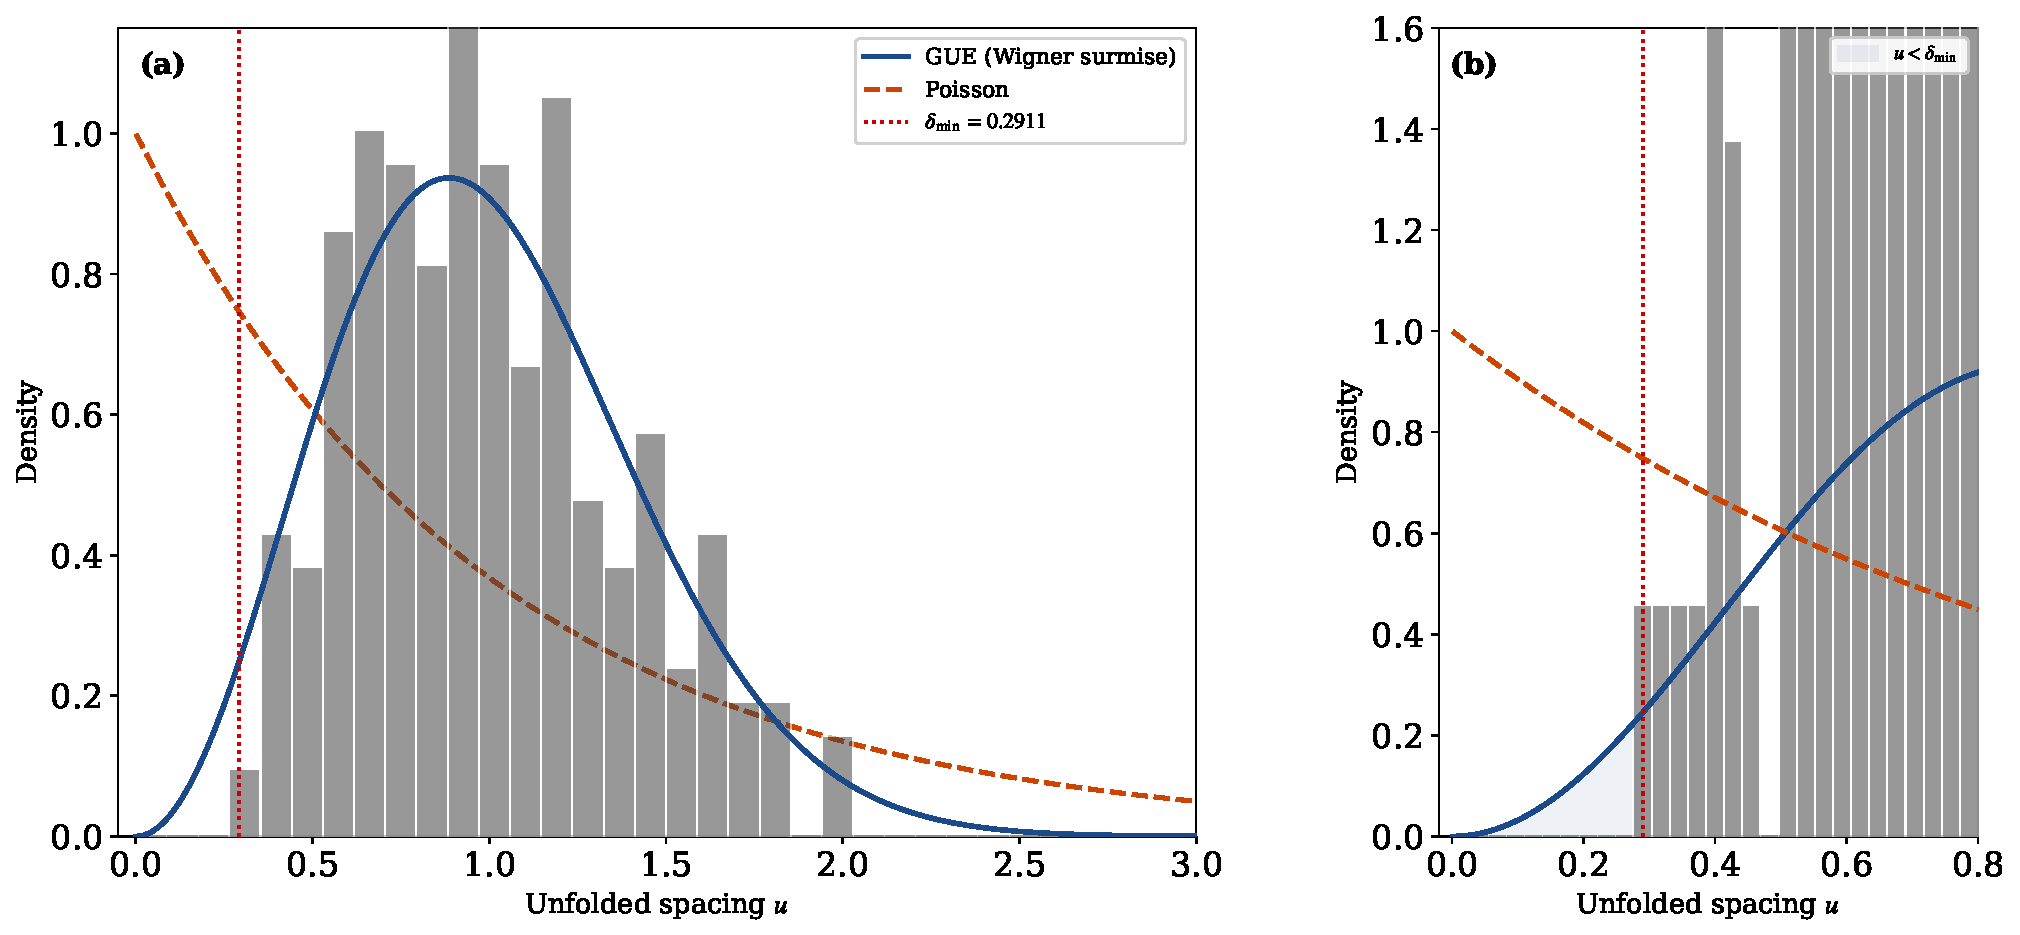
\includegraphics[width=\linewidth]{fig7_spacing_histogram.pdf}
\caption{Level repulsion in $\zeta$ zeros (Def.~\ref{def:repulsion}): (a) histogram of $237$ unfolded spacings ($\gamma_1{=}14.13$ to $\gamma_{238}{=}453.99$) against the GUE Wigner surmise and the Poisson exponential; (b) zoom on the repulsion region, with $\delta_{\min}{=}0.2911$ marked. The shaded zone $u{<}\delta_{\min}$ is where GUE suppresses spacings that Poisson permits.}
\label{fig:spacing-histogram}
\end{figure}

\begin{proposition}[Repulsion excludes the extreme case]\label{prop:repulsion-excludes}
If $Z$ repels at some $m>0$ then no two distinct elements share an ordinate; and since off the line
the pair $\{\rho,\sigma\tau(\rho)\}$ has separation exactly zero
(Proposition~\ref{prop:arity-two}), every $\rho\in Z$ closed under $\sigma\tau$ satisfies
$\Re\rho=\golden^{-\lng}$. The configuration the ensemble makes improbable and the one repulsion
excludes are the same configuration.
\P{repulsion_excludes_zero_spacing, repulsion_excludes_the_extreme_case}
\end{proposition}

\begin{theorem}[The weak form, and what would suffice]\label{thm:weak-form}
Closure under $\sigma\tau$ alone gives
\begin{equation}\label{eq:E-iff-no-sharing}
  \bigl(\forall\rho\in Z:\ \Re\rho=\golden^{-\lng}\bigr)
  \iff \text{no two distinct elements of } Z \text{ share an ordinate}.
\end{equation}
The right-hand side is strictly weaker than Definition~\ref{def:repulsion}: repulsion implies it,
not conversely. It is what any future argument would discharge in place of the metric bound.
\P{E_iff_no_shared_ordinate}
\end{theorem}

\begin{proposition}[Repulsion gives the modulus]\label{prop:repulsion-modulus}
Under the same hypotheses, $\lvert1-1/\rho\rvert=1$ exactly. The measured repulsion does not merely
constrain the modulus: it \emph{produces} it.
\P{repulsion_gives_the_modulus}
\end{proposition}

\begin{theorem}[Zeros on the apex, with its inputs in view]\label{thm:zeros-apex}
Let $Z\subset\C$ be closed under $\sigma\tau$ and repel at some $m>0$
(Definition~\ref{def:repulsion}). Then every $\rho\in Z$ satisfies $\Re\rho=\golden^{-\lng}$, the
apex of Theorem~\ref{thm:mu-diagram}.

Two inputs are open and are named here rather than hidden. Closure needs the conjugation half of
\eqref{eq:sdual-mate}, $\xi(\bar s)=\overline{\xi(s)}$, not established in this paper \Conj; and
the repulsion is measured . Everything between them is proved, and of the measurement only \N{eq:sdual-mate}
the \emph{sign} enters.
\end{theorem}

\begin{remark}[What the argument does not use]\label{rmk:no-statistics}
Theorem~\ref{thm:zeros-apex} uses the geometry of $\C$ and the sign of one bound. It uses no
joint density, no sine kernel, no form factor, no asymptotic statistics of the spacings. That is
the point of stating the extreme case at arity two: the exclusion the criterion needs is about
\emph{one pair}, and a pair is an individual. Where the ensemble was standing in for an object,
the object here is the modulus, and what the statistics described is a consequence of its
geometry rather than a substitute for it. The chain that discharges the two open inputs, and the
measured bound itself, belong to the companion papers~\cite{HP,F1}; note that they are stated
there for $L(s,\chi_5)$, whose functional equation is a different theorem from
\eqref{eq:funct-eq}, proved separately in~\cite{F1}.
\end{remark}


\begin{definition}[The ensemble's own object]\label{def:pair-correlation}
The statistics invoked in \S\ref{sec:intro} are those of the GUE pair-correlation kernel
\begin{equation}\label{eq:sine-kernel}
  K(u)=1-\Bigl(\frac{\sin\pi u}{\pi u}\Bigr)^{2} .
\end{equation}
It is written here---the attribution is at \S\ref{sec:intro}---so that the object the paper opened
with is a node of this development rather than a gap in it. It vanishes as $u\to0$, which is the
suppression of small spacings that Definition~\ref{def:repulsion} measures, and tends to $1$ for
large $u$, which is decorrelation. Nothing below uses it. \Conj
\end{definition}

\begin{figure}[htb]\centering
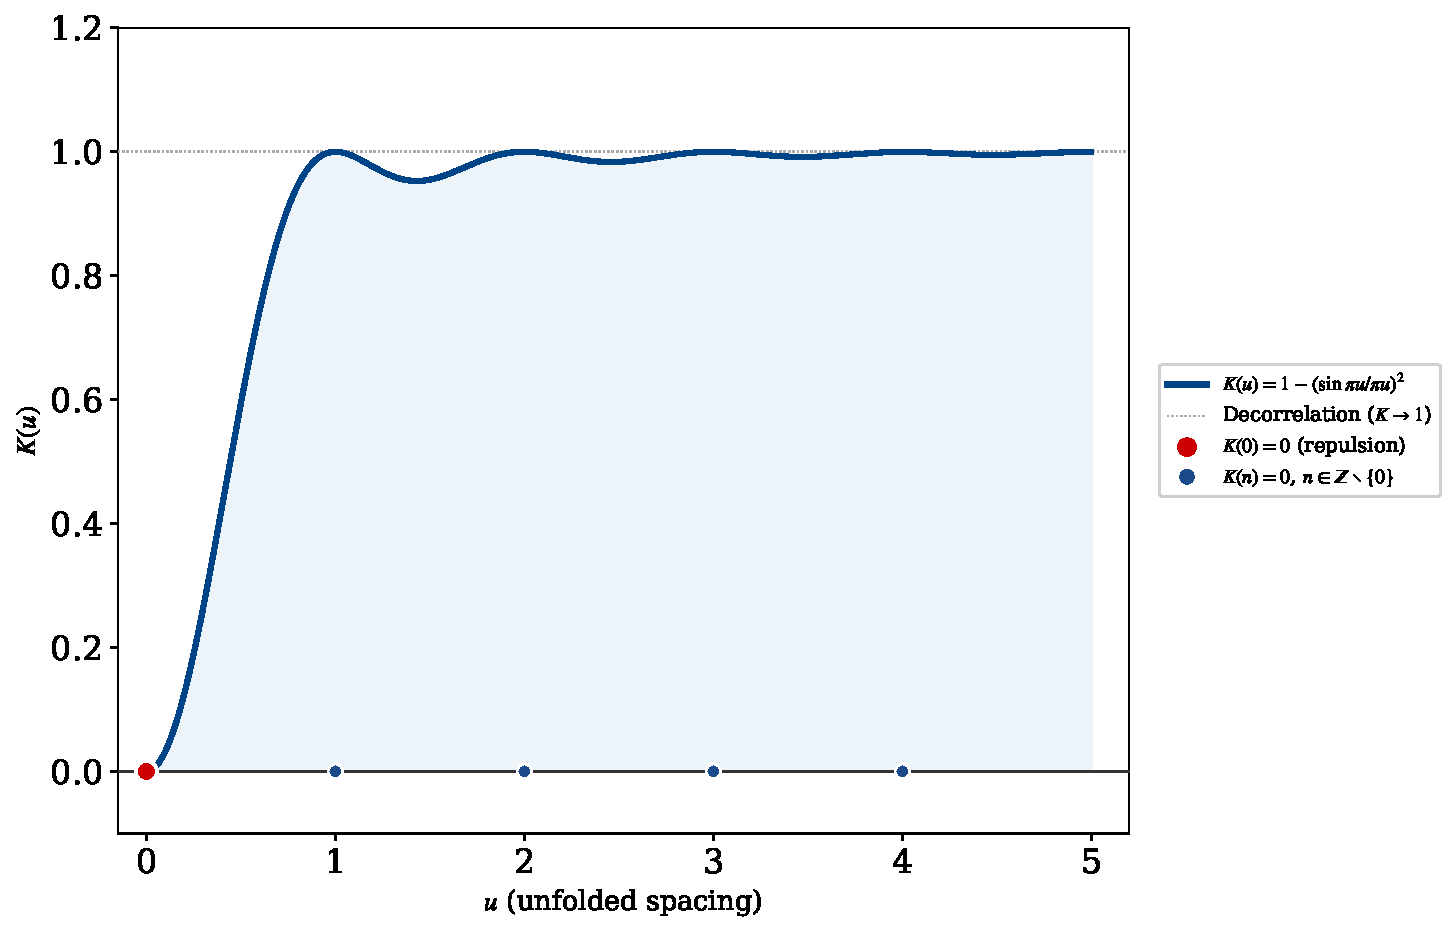
\includegraphics[width=\linewidth]{fig8_sine_kernel.pdf}
\caption{The GUE pair-correlation kernel $K(u)=1-(\sin\pi u/\pi u)^{2}$ of Def.~\ref{def:pair-correlation}. The red point at $K(0){=}0$ is level repulsion---the suppression of small spacings that Def.~\ref{def:repulsion} measures. Blue points mark $K(n){=}0$ for $n\in\Z\setminus\{0\}$ (no long-range correlation). The kernel tends to $1$ for large $u$ (decorrelation).}
\label{fig:sine-kernel}
\end{figure}

\begin{remark}[Envelope yes, fluctuations no]\label{rmk:envelope-not-fluctuations}
The ensemble stands on a distinction between the smooth spectral density and the fluctuations
around it. A deterministic operator built without reference to $\zeta$ determines the
envelope---the global distribution of zeros---but the pair-correlation statistics reside in the
fluctuations, and reproducing them would require either an exact spectrum or a dynamical mechanism
generating the level repulsion of Definition~\ref{def:repulsion}. \emph{This is intrinsic to the
construction, not a gap in the work}: it is why the present subsection proves a statement about
\emph{one pair} rather than about a distribution. The joint density and the form factor are
declared in the development and used in no signature; that is the check that nothing here rests on
them. \Empty
\end{remark}

\begin{remark}[A geometric origin for the constraint]\label{rmk:geometric-origin}
What the framework does supply is a candidate \emph{origin} for the constraint that makes such
statistics possible, and it is already proved above: the ratio $\sigma/\mu$ is the arity $d=3$
(Remark~\ref{rmk:spectral-origin}), the modulus contracts strictly, $\|\hat\Omega\|=\tfrac12<1$
(Remark~\ref{rmk:no-diagonal}), and the same $3$ is the exponent of
$\prod_k\lvert\lambda_k\rvert=2^{-3}$ in Proposition~\ref{prop:triad-invariants}. The reading that
eigenvalue correlations in this regime arise from \emph{geometric constraint}---the no-diagonal
condition---rather than from dynamical instability is advanced in the companion paper~\cite{HP};
it is a proposal there and not a theorem here, and is recorded as such. What is established in
this section is the regime, not the reading. \Open
\end{remark}

\begin{remark}[Not the tower spacing]\label{rmk:not-the-tower-spacing}
One caution, now that spacings are in play: the tower has its own spacing, the regulator
$R_K=\log\golden$ of \eqref{eq:regulator}, numerically $0.481212$, while the unit that unfolds
ordinates at $T=100$ is $1.435589$ (Proposition~\ref{prop:scale}). They share the symbol $\golden$
and are different objects.
\P{tower_spacing_is_the_regulator}
\end{remark}

% ---------------------------------------------------------------------
\subsection{Formal verification}\label{ssec:status}

Each result of this section carries, in brackets, the name of its Lean~4
theorem. The development that accompanies the paper is the self-contained
file \texttt{CW6\_complete\_v2.lean}. It compiles under \texttt{leanprover/lean4}~v4.29.0 with
Mathlib~v4.29.0: \texttt{lake build} completes with no errors and no warnings, and the file
declares \emph{no} \texttt{axiom} and contains no \texttt{sorry}. The file closes with the
framework colimit of \S\ref{ssec:web} below (namespace \texttt{PCFColimit}): the frameworks the paper
treats---Polyakov, Maldacena, ER$=$EPR, Huerta--Schreiber, Kiely---as partial spectral objects
together with the PCF core, whose fields are populated by theorems of this same file
(\texttt{modulus\_Omega}, \texttt{holographic\_area}, \texttt{kk\_at\_PCF},
\texttt{two\_pow\_hausdorff}, the P/C/F norms), the cocone into the vertex $T_{\PCF}$
(\texttt{cocone\_property}), and the universal property that makes the vertex unique
(\texttt{colimit\_universal}, \texttt{framework\_colimit}).
The external results the file uses
enter as explicit hypothesis arguments in the types of the theorems that consume them---where
the reader can see them---rather than as axioms; the classical analytic inputs
(\texttt{gammaR\_from\_tate}, \texttt{theta\_from\_jacobi}) and the combinatorial ones
(\texttt{ladder\_from\_scott}, \texttt{e8\_dim\_from\_kissing}, \texttt{positroid\_from\_kp},
\texttt{no\_separable\_parts}) are carried that way. Two further inputs enter the same way in
\S\ref{ssec:extreme} and are recorded here because they are the only open ones in that
subsection: \texttt{XiConjClosed}, the closure $\xi(\bar s)=\overline{\xi(s)}$ of the zeros
under conjugation, which is \emph{not} established in this paper \Conj; and
\texttt{MinSpacing}, a positive minimal ordinate separation, which is measured rather than
proved . Of the second only its sign is used. Neither is an axiom: both are hypothesis \N{thm:zeros-apex}
arguments in the type of Theorem~\ref{thm:zeros-apex}. One decision procedure uses
\texttt{native\_decide} rather than \texttt{decide}---the sweep of $16\times17\times18$ triples behind
Proposition~\ref{prop:interval-uniqueness}---which extends the trusted base to Lean's compiler
as well as its type kernel; every other proof rests on the kernel alone. The golden ratio is
defined, $\golden:=(1+\sqrt5)/2$, and the two facts that anchor the
construction are theorems proved from that definition, not assumptions. The
relation $\golden^2=\golden+1$ (\texttt{phi\_sq}) is derived from the
definition and is~\eqref{eq:phisq}. The modulus $\|\hat\Omega\|=\tfrac12$
(\texttt{modulus\_Omega}) is likewise a theorem. Its value is reached by the routes assembled in
Theorem~\ref{thm:mu-diagram}, its component structure is
Proposition~\ref{prop:pcf-norms}, and the trigonometric collapse of the norm product is
Theorem~\ref{thm:collapse}; the three quantities that coincide there and cease to coincide
afterwards are separated in Proposition~\ref{prop:triad-invariants}.

\smallskip
\sloppy\noindent\textbf{Compilation note (single point of record).} The development declares no
axiom: every classical input is a hypothesis argument in the type of the theorem that consumes it.
\texttt{lake build} completes against Mathlib, confirming the spelling
of every library lemma the proofs call. The lemma names, grouped by what they serve,
are recorded here so that a future Mathlib rename breaks the build visibly rather than
passing silently:
\begin{itemize}\itemsep1pt\parskip0pt
\item \emph{Completed zeta and the places} (\S\ref{ssec:zeta}): \texttt{Gamma}$_\R$,
  \texttt{Gamma}$_\R$\texttt{\_ne\_zero\_of\_re\_pos}, \texttt{riemannZeta\_def\_of\_ne\_zero},
  \texttt{zeta\_eq\_tsum\_one\_div\_nat\_cpow}, \texttt{riemannZeta\_eulerProduct\_tprod},
  \texttt{completedRiemannZeta\_one\_sub}, \texttt{integral\_gaussian}, \texttt{Real.sq\_sqrt},
  \texttt{Real.Gamma\_eq\_integral}.
\item \emph{The generator and its conjugate} (\S\ref{ssec:generator}), \emph{the arithmetic
  seed} (\S\ref{ssec:origins}) \emph{and the cocone} (\S\ref{ssec:commute}):
  \texttt{Real.sq\_sqrt}, \texttt{Real.Gamma\_add\_one}, \texttt{Real.Gamma\_pos\_of\_pos}.
\item \emph{The eigenvalue triad} (Proposition~\ref{prop:triad-invariants}):
  \texttt{Complex.exp\_ofReal\_mul\_I\_re}, \texttt{Complex.exp\_nat\_mul},
  \texttt{Complex.exp\_two\_pi\_mul\_I}, \texttt{Real.cos\_pi\_sub},
  \texttt{Real.rpow\_mul}, \texttt{Real.rpow\_natCast}, \texttt{Real.rpow\_neg}.
\item \emph{The companion and the extreme case} (\S\ref{ssec:extreme}): \texttt{map\_sub},
  \texttt{map\_one} on \texttt{starRingEnd}, \texttt{Complex.conj\_re},
  \texttt{Complex.conj\_im}, \texttt{Complex.ext\_iff}.
\item \emph{Theta and Poisson} (\eqref{eq:theta-lattice}):
  the file defines \texttt{Theta} directly without Mathlib's \texttt{jacobiTheta}.
\item \emph{Pentagon and Fibonacci} (\S\ref{ssec:spectrum}, \S\ref{ssec:tower}):
  \texttt{Real.cos\_pi\_sub}, \texttt{Real.cos\_two\_mul}, \texttt{Nat.fib}.
  The general form of \eqref{eq:fib-criterion} would need Frobenius in \texttt{ZMod q}; it is
  stated here by cases.
\item \emph{Even zeta values} (Theorem~\ref{thm:even-zeta}): the name of the even-value lemma,
  and \textbf{whether it is stated with \texttt{bernoulli} or with \texttt{bernoulli'}}. The two
  differ only at $B_1$ and agree at every even index $\ge2$, so the statement is the same either
  way; the identifier is not.
\item \emph{Group orders} (Lemma~\ref{lem:s3-orders}): the index-two fact for $A_n$,
  \texttt{two\_mul\_card\_alternatingGroup} or its equivalent.
\item \emph{Matrices} (Theorem~\ref{thm:faces}): \texttt{Matrix.mul\_inv\_rev},
  \texttt{Matrix.transpose\_nonsing\_inv}.
\item \emph{Earlier blocks}: \texttt{Gamma\_one\_half\_eq}, \texttt{riemannZeta\_two},
  \texttt{Real.sqrt\_eq\_rpow}, \texttt{rpow\_natCast}, \texttt{Gamma\_add\_one},
  \texttt{arccos\_cos}, and for the M6 uniqueness \texttt{Nat.Prime.irrational\_sqrt},
  \texttt{Irrational.intCast\_mul}, \texttt{Int.not\_irrational}.
\end{itemize}
\noindent Since \texttt{lake build} completes, any renaming or removal of these lemmas in a
future Mathlib breaks the build rather than passing silently. The numerical companion is the
pytest suite in \PytestInline{tests/} (run via \texttt{pnpm run verify:py}),
whose tests are keyed by the \TeX{} labels of this file: of the $162$ labelled equations,
$148$ carry a Lean proof and $119$ a numerical check, $102$ carrying both---the tests evaluating
identities at up to $25$-digit precision and, where a claim is a correspondence with measurement,
comparing against the measured value. The eight carrying neither a proof nor a check of their
own are the five correspondence statements \eqref{eq:bridge-S}--\eqref{eq:bridge-ER} plus
\eqref{eq:dS-swampland}; \eqref{eq:cnf} whose Lean form is the hypothesis
\texttt{hCNF} of \texttt{L1\_from\_class\_number\_formula};
the Polyakov action \eqref{eq:polyakov} (an  input); and the \Hyp{}
Lawvere--Yanofsky diagonal \eqref{eq:LY}, which states the problem rather than a result.
The global Dedekind factorisation \eqref{eq:dedekind} is counted among the $147$: its Lean
backing sits at the local factors \eqref{eq:local-dedekind} that compose it. The figures are generated by
\texttt{CW6\_all\_figures\_v2.py} and their assertions checked, separately and against the labels of
this file, by \texttt{CW6\_figures\_verify\_v2.py}.


% ===================================================================

\section{Derivations}\label{sec:derivations}

Building on the single microstate established in \S\ref{sec:methods}, this section
presents one demonstrative line: the object generates a tower, and the tower generates
the duality web. The line runs in the order $3.1\to3.2\to3.3\to3.4\to3.5$, summarised as a
$20$-step spine at the end (\S\ref{ssec:spine}). The node that stitches \S\ref{sec:methods}
to here is the function $\Gamma$; every quantitative statement below is verified numerically
at $25$-digit precision where the identity requires it (\S\ref{ssec:status}).

% --- 3.1 ---
\subsection{The fundamental object in physics}\label{ssec:object}
The single object is the half-integer $\Gamma$ value, the carrier of the string microstate.
The seed inherited from \S\ref{sec:methods} is
\begin{equation}\label{eq:gamma-half}
  \Gamma\!\left(\tfrac12\right)=\sqrt{\pi}.
\end{equation}
The worldline phase and its modulus are
\begin{equation}\label{eq:worldline}
  \Om(\tau)=\tfrac12\,e^{\,i\tau\ln\golden},\qquad |\Om|=\tfrac12 .
\end{equation}
The wavefunction is Gaussian, with the half-factorial normalisation $\Gamma(\tfrac12)=\sqrt\pi$
and a weight fixed by the scale quantum,
\begin{equation}\label{eq:gaussian}
  \int_{\R} e^{-x^{2}}\,dx=\sqrt{\pi},\qquad
  \mu=\golden^{-\lng}=\tfrac12\quad(\golden^{\lng}=2).
\end{equation}

\begin{remark}[The wavefunction is the self-dual Gaussian]\label{rmk:wf-selfdual}
The Gaussian weight of \eqref{eq:gaussian} is the self-dual one fixed in
\S\ref{ssec:origins}, Proposition~\ref{prop:selfdual-gaussian}: normalised, and equal to its own
Fourier transform, $g(x)=e^{-\pi x^{2}}$ \eqref{eq:selfdual-gaussian}. The physical reading added
here is that this $g$ is the worldline wavefunction of the microstate; the width is not a
modelling choice but the fixed point of the Fourier transform, the same self-duality that
\S\ref{ssec:construction} used to fix $\tau=i$. \ProofWitness{selfdual\_gaussian\_unique}

\end{remark}

The one-dimensional worldline is promoted to the two-dimensional worldsheet, governed by the
Polyakov action~\cite{Polchinski98}
\begin{equation}\label{eq:polyakov}
  S_{P}=-\frac{1}{4\pi\alpha'}\int d^{2}\sigma\,\sqrt{-h}\;
        h^{ab}\,\partial_{a}X^{\mu}\,\partial_{b}X^{\nu}\,\eta_{\mu\nu}.
\end{equation}
% \HypWitness{}

\begin{proposition}[The worldsheet inherits the non-orientable fibre]\label{prop:mobius}
The worldsheet carries the non-orientable fibre of the base torus
(Proposition~\ref{prop:mobius-torus}, \S\ref{ssec:mobius-torus}): the module direction of
$\Om(\tau)=\tfrac12\,e^{\,i\tau\ln\golden}$~\eqref{eq:worldline}, carried once around the fundamental
domain, closes with the orientation-reversing half-turn $e^{i\pi}=-1$. The worldsheet is therefore
non-orientable and one-sided---the half-turn carries the module's interior edge to its exterior---so
the bulk--boundary relation the torus carries admits no privileged side, independently of which torus
carries the fibre.
\ProofWitnessBlock{fibre\_monodromy, fibre\_reflection\_order\_two, fibre\_independent\_of\_base}
\end{proposition}

The Schwinger parametrisation, used to assemble propagators and amplitudes, follows from the
$\Gamma$ integral by the change of variable $t=xA$,
\begin{equation}\label{eq:schwinger}
  A^{-n}=\frac{1}{\Gamma(n)}\int_{0}^{\infty}x^{\,n-1}\,e^{-xA}\,dx\qquad(A>0,\ n>0).
\end{equation}

\begin{remark}[The role of $\golden$ in the object]
Since $\pi=5\arccos(\golden/2)$ (\S\ref{sec:methods}), both $\sqrt\pi$ and the half-factorial
are functions of $\golden$; and $\mu=\tfrac12=\golden^{-\lng}$. The object is $\golden$-generated,
not posited.
\end{remark}

% --- 3.2 ---

\subsection{The meta-invariant: the holographic quantum}\label{ssec:meta}
The meta-invariant emerges from the structure already in place: the worldsheet phase
$\Om(\tau)=\tfrac12\,e^{\,i\tau\ln\golden}$ of \S\ref{ssec:object}~\eqref{eq:worldline},
carried on the torus $T^2_{\PCF}$ of \S\ref{ssec:construction}~\eqref{eq:torus}, whose single
modulus $|\Om|=\tfrac12$ is the norm product fixed in
\S\ref{ssec:construction}~\eqref{eq:omega-norms}. The bridge from this object to the rest of
physics is that $|\Om|=\tfrac12$ \emph{is} the holographic bit (one bit per Planck area); that this
bit is the regulator of $\Q(\sqrt5)$ measured in $\lambda_{\log}$, and not a coincidence with
$\mu_3$, is Theorem~\ref{thm:entropy-bridge}. The
spectral invariants are
\begin{equation}\label{eq:spectral-invariants}
  d=3\;(=|S_{3}|=3!=6),\qquad \mu=\tfrac12,\qquad \sigma=\tfrac32,\qquad \sigma+\mu=2 .
\end{equation}
The two $\tfrac32$'s of the corpus---the $\Gamma$ argument of \eqref{eq:half-factorial} and the
spectral exponent here---are one value for a discriminating reason: the first is $1+\mu$, the
second $3\mu$, and $1+\mu=3\mu$ has the unique solution $\mu=\tfrac12$; at arity $n$ the Basel
route \eqref{eq:sigma-basel} gives $n^{2}/6$, which meets $\tfrac32$ only at $n=3$. \ProofWitness{three\_halves\_unique, arity\_control\_three}

\paragraph{The spectral angle and the uniqueness of the invariants.}
At scale $\sigma$ the worldline subtends the spectral angle
$\alpha(\sigma)=\arctan(\epsz\golden^{\sigma})$, normalised by $\epsz M_{\PCF}=\pi$.
The invariants \eqref{eq:spectral-invariants} are not chosen but
forced: the pair $(\sigma,\mu)$ with $\sigma+\mu=2$ and $\sigma\mu=\tfrac34$ has the unique
solution $(\sigma,\mu)=(\tfrac32,\tfrac12)$,
i.e.\ $\sigma=\tfrac32$
the same arity $3$ and modulus $\tfrac12$ forced by the No-Diagonal theorem
of \S\ref{ssec:arity}. Which \emph{integer} levels the angle is read at is not settled here: it is
fixed by the level interval of \S\ref{sec:implications}, Proposition~\ref{prop:interval-uniqueness}.

\begin{proposition}[The tangent of the spectral angle is the tower]\label{prop:spectral-angle-tower}
For every $\sigma$,
\begin{equation}\label{eq:spectral-angle}
  \tan\alpha(\sigma)=\epsz\golden^{\sigma},
  \qquad\text{hence}\qquad
  \frac{\tan\alpha(\sigma+1)}{\tan\alpha(\sigma)}=\golden ,
\end{equation}
so the angle is not an auxiliary parameter: its tangent is the multiplicative spectrum that
$\golden$ generates, climbing at the one rate $\golden$ of \eqref{eq:base} --- the same spectrum
\S\ref{ssec:p-tower} will read as the tower. The surface
$\sin\alpha(\sigma_1)\cos\alpha(\sigma_2)$ has the closed form
\begin{equation}\label{eq:spectral-surface}
  \sin\alpha(\sigma_1)\cos\alpha(\sigma_2)
  =\frac{\epsz\golden^{\sigma_1}}
        {\sqrt{\bigl(1+\epsz^{2}\golden^{2\sigma_1}\bigr)\bigl(1+\epsz^{2}\golden^{2\sigma_2}\bigr)}} .
\end{equation}
What the certainty principle $\epsz\Mpcf=\pi$ \eqref{eq:certainty} contributes is the
\emph{scale} of the argument, $\epsz=\pi/\Mpcf$, and nothing else: the bound
$\alpha(\sigma)<\pi/2$ is a property of $\arctan$ and holds for every real argument, so it is
not the certainty relation that keeps the angle off the right angle. The bound is used for one
thing---it gives $\cos\alpha(\sigma)>0$, the hypothesis under which
Corollary~\ref{cor:bridge-angle} divides by $\cos\alpha$. \ProofWitness{spectral\_angle\_tan, spectral\_angle\_tower\_ratio}

\end{proposition}
\begin{proof}
$\tan\arctan x=x$ with $x=\epsz\golden^{\sigma}>0$ gives the first identity, and the quotient of two
consecutive values is $\golden^{(\sigma+1)-\sigma}=\golden$, the $\epsz$ cancelling. For
\eqref{eq:spectral-surface}, $\sin\arctan x=x/\sqrt{1+x^{2}}$ and $\cos\arctan y=1/\sqrt{1+y^{2}}$;
multiplying the two gives the display. The bound is $\arctan x<\pi/2$ for all finite $x$.
\end{proof}
With the binary entropy $H(p)=-p\log_{2}p-(1-p)\log_{2}(1-p)$, the modulus saturates the
Bekenstein bound~\cite{Bekenstein73,Hawking75},
\begin{equation}\label{eq:bridge-BH}
  \frac{1}{4\GN}=\tfrac12=|\Om|,\qquad H\!\left(\tfrac12\right)=1\ \text{bit},\qquad
  \SBH=\frac{A}{4\GN}.
\end{equation}

\begin{remark}[The role of $\golden$ in the meta-invariant]
$\mu=\tfrac12=\golden^{-\lng}$ is the scale quantum ($\golden^{\lng}=2=$ one bit). The invariants
$d=3,\ \mu=\tfrac12,\ \sigma=\tfrac32$ come from the $\golden/S_{3}$ geometry of
\S\ref{sec:methods}; they are not postulated.
\end{remark}

\paragraph{Thread (the invariants force the holographic principle).}
The holographic principle is read off the invariants, not assumed:
\begin{enumerate}
  \item the modulus $\mu=\tfrac12=|\Om|$ has binary entropy $H(\tfrac12)=1$, so each fundamental
        cell (each eigenvalue) carries exactly one bit
        (\eqref{eq:spectral-invariants}$\to$\eqref{eq:bridge-BH});
  \item the $d=3$ eigenvalues give $3$ bits $=c=3$ (Brown--Henneaux~\cite{BrownHenneaux86}: three eigenvalues $\times$
        one bit);
  \item and $1/(4\GN)=\mu=\tfrac12$ turns $\SBH=A/(4\GN)$ into the area law.
\end{enumerate}
Hence information $=$ one bit per Planck area (the holographic bound), read from the invariants.
(Numerically verified: \eqref{eq:certainty}, \eqref{eq:obs-interface}, \eqref{eq:brown-henneaux}.)

This is the holographic bound that Susskind, following 't~Hooft, drew from unproven
assumptions about the nonperturbative behaviour of string theory: one discrete degree of
freedom per Planck area~\cite{Susskind95,SusskindWitten98}. Here it is not assumed but
derived---the bit $H(\tfrac12)=1$, the central charge $c=3$, and the area law
$\SBH=A/4\GN$ are read off the single modulus $|\Om|=\tfrac12$.

% --- 3.3 ---

\subsection{The object as generator of the tower and the amplitudes}\label{ssec:p-tower}
Built on the golden tower of \S\ref{ssec:tower} (the Borger $\Lambda$-structure on
$\golden^{\sigma}$) and the mediated spectrum of \S\ref{ssec:spectrum}, the tower mediates
\emph{between} a binary register (the half-factorial $/\,\Gamma\,/\,\pi$;
$i$, $d{=}1{\to}2$) and a ternary one ($S_{3}/\golden$; $d{=}2{\to}3$), with $\mu=\tfrac12$ as
the geometric mean. The Huerta--Schreiber superpoint is purely binary ($\Z_{2}$)
\cite{huerta2018m}; PCF spans and mediates both. The relation is sharper than a contrast of
registers. The binary $\Z_{2}$ of the superpoint is not isolated in the framework: the binary
register and the turn are one object, since $2$ satisfies in $\F_5$ the equation $i$ satisfies in
$\C$ \eqref{eq:two-is-i} and is its image under the reduction at a prime over $5$
(Proposition~\ref{prop:four-cocone}). Its fourth order is therefore one of the two factors of the
conductor $20$ derived in \S\ref{ssec:spacings}, the other being the $5$ of the pentagon
(Theorem~\ref{thm:pentagon-id}), the two being coprime so that
$\operatorname{lcm}(4,5)=20$~\eqref{eq:conductor}. The $\Z_{20}$ that decides $\chi_5$
\eqref{eq:fib-criterion} therefore factors as $\Z_{4}\times\Z_{5}$, and each factor governs one
character and only one \eqref{eq:attribution}, neither determining the other
(Proposition~\ref{prop:attribution}): the binary side of the
superpoint and the pentagonal side of $\golden$ are its two components. That is the precise sense
in which PCF mediates rather than merely spans---the two registers are not juxtaposed but are the
coprime factors of a single conductor, and the mediation $\mu=\tfrac12$ of
\eqref{eq:tower-mediation} below is the geometric mean between them.
The M-theory object enters here: the HS tower
projects from the $\golden^{\sigma}$ tower. The dimensional chain is
\begin{equation}\label{eq:dim-chain}
  \R_{d=1}\xrightarrow{\;i^{2}=-1\;}\C_{d=2}
  \xrightarrow{\;\golden^{2}=\golden+1\;}\E^{3}_{d=3}.
\end{equation}
Mediation by $\mu=\tfrac12$ produces the two registers,
\begin{equation}\label{eq:tower-mediation}
  \golden^{\,\mu\lng}=\sqrt{2}\ \ (\text{binary}),\qquad
  \golden^{\,\mu\log_{\golden}3}=\sqrt{3}\ \ (\text{ternary}).
\end{equation}
\ProofWitnessBlock{M4\_sqrt2, M4\_sqrt3}
The tower and its mode count are
\begin{equation}\label{eq:tower-modes}
  z(\sigma)=\golden^{\sigma},\qquad \Nmodes(\sigma)=\big\lfloor\pi\,\golden^{\sigma}\big\rfloor .
\end{equation}
This is where the geometric encoding replaces the Fourier expansion of the string as the
device that fixes the mode content: \eqref{eq:tower-modes} counts modes by the cell capacity
$\pi$ of \eqref{eq:certainty} at each level of the tower rather than by harmonic order. The
two are not in conflict---the count is finer-grained, and it is tied through
\S\ref{ssec:adscft} to the information the horizon carries.

\begin{remark}[Fibonacci-adjacent, and where it parts company]\label{rmk:fib-adjacent}
The count \eqref{eq:tower-modes} is \emph{adjacent} to the Fibonacci sequence, not equal to it:
$\lvert\Nmodes(\sigma)-F\rvert\le1$ for the nearest Fibonacci $F$, with equality
$\Nmodes(\sigma)=F$ for $\sigma\le5$ --- the values $3,5,8,13,21,34$ --- and a genuine departure at
the tower ceiling, where $\Nmodes(6)=\lfloor\pi\golden^{6}\rfloor=56$ while the Fibonacci value is
$55$. The distinction matters: the factor $\pi$ of \eqref{eq:tower-modes} is the cell capacity of
\eqref{eq:certainty} and not a Fibonacci index, so the staircase is $\pi$-scaled and only
\emph{shadows} the recurrence of Theorem~\ref{thm:fib-min}. Reading the tower as Fibonacci would
put $55$ at the tower ceiling $\sigma=2n$, where the saturation entropy is largest. \ProofWitness{fib\_adjacent\_le\_one, Nmodes\_six\_ne\_fib} \NumericalWitness{thm:fib-min}

\end{remark}

\begin{remark}[The scale operator of the tower, and which spectrum is which]\label{rmk:mass-operator}
The tower $z=\golden^{\sigma}$ of \eqref{eq:tower-modes} defines the diagonal scale operator
\begin{equation}\label{eq:mass-operator}
  H\lvert\sigma\rangle=m_0\,\golden^{\sigma},\qquad
  \mathrm{spec}\,H=\{0\}\cup\{m_0\golden^{\sigma}\}_{\sigma\ge0},
\end{equation}
self-adjoint (real diagonal) and bounded below, with the vacuum at $0$; its gap and the reconstruction
it supports are established in \S\ref{sec:dof}. \ProofWitness{towerHam\_isHermitian, towerHam\_bounded\_below}

Two spectra must be kept apart here, and the framework supplies both from the same pair $\pi,\golden$.
The golden tower \eqref{eq:tower-modes} is the \emph{radial and scale} tower: its successive ratio
tends to $\golden$ and its physical mass reading is the Kaluza--Klein one, the interior KK mass
carrying the golden identity $\golden^{2}+\golden^{-2}-2=1$ (\S\ref{app:kk},
\eqref{eq:kk-numerator})---the gravity side. The \emph{confining} mass spectrum, on the gauge side, is
the Regge tower $\alpha'M_n^{2}=n$ of \eqref{eq:veneziano}, whose integer pole positions index the
Dirichlet series \eqref{eq:euler-product} and hence $\zeta$; its mass ratios are therefore
$M_n/M_1=\sqrt n$, not $\golden^{\sigma}$. The two are distinct spectra but not unrelated: the constant of the confining tower is the Regge slope $\alpha'$, the string tension $T=1/2\pi\alpha'$, and \S\ref{sec:dof} shows this tension welded to the golden tower level by level---so the radial and confining towers are two readings of one scale, related through the tension rather than conflated.
\end{remark}
\begin{figure}[!htbp]\centering\n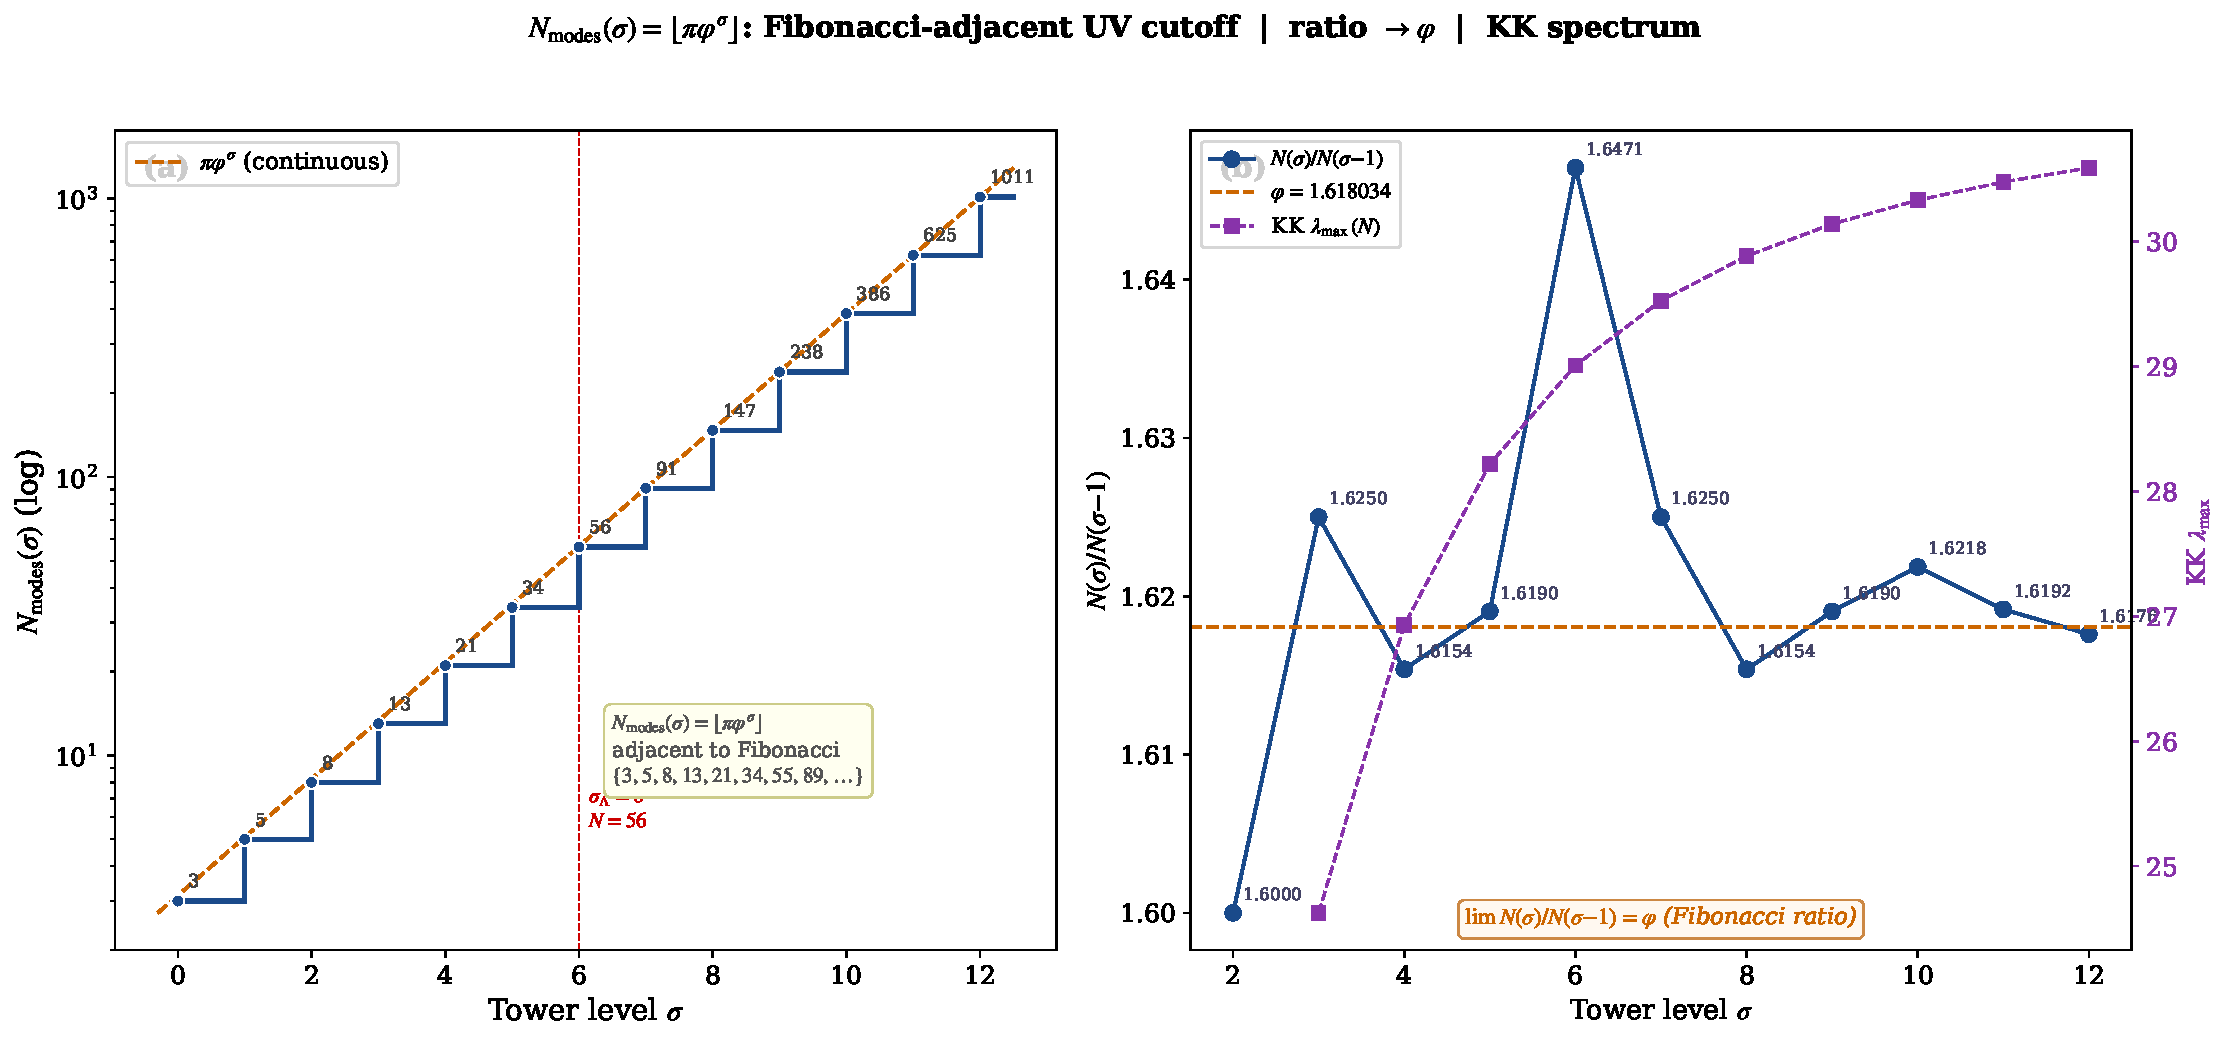
\includegraphics[width=\linewidth]{fig3_N_modes.pdf}
\caption{The mode tower $\Nmodes(\sigma)=\lfloor\pi\golden^{\sigma}\rfloor$ \eqref{eq:tower-modes}:
(a) the Fibonacci-adjacent staircase $\{3,5,8,13,21,34,56,\dots\}$, equal to the Fibonacci values
for $\sigma\le5$ and departing at $\sigma=6$ where $56\neq55$
(Remark~\ref{rmk:fib-adjacent}); (b) the successive ratio
$\Nmodes(\sigma)/\Nmodes(\sigma-1)\to\golden$ alongside the Kaluza--Klein spectrum.}
\label{fig:tower-modes}
\end{figure}
The Huerta--Schreiber brane-bouquet tower~\cite{huerta2018m} maps to the PCF tower under a functor $F$,
\begin{equation}\label{eq:HS-tower}
  \R^{0|1}\to\R^{1,1|1}\to\cdots\to\R^{9,1|16}\to\R^{10,1|32}
  \ \xrightarrow{\;F\;}\ \{\golden^{\sigma}\}_{\sigma},
\end{equation}
the dynamics being presupposed on the HS side ($H=L_{0}+\bar L_{0}$) and derived on the PCF side.
Both sides are chains, so $F$ is the order-preserving level map---superpoint\,$\to$\,NS5 at
$\sigma=0,\dots,5$ on the hypercube $H_5$ (\S\ref{ssec:adscft}, App.~\ref{app:superpoint})---and
what it carries is the modulus, $|\Om|=\tfrac12$, $|\Om|^{2}=\tfrac14$, proved at the corner
(App.~\ref{app:web}).
Tree amplitudes follow from $\pi$ (binary, via $\Gamma$) and $\golden$ (ternary, via Regge): the
Veneziano amplitude \cite{Veneziano}
\begin{equation}\label{eq:veneziano}
  A_{4}=\frac{\Gamma(-\alpha's)\,\Gamma(-\alpha'u)}{\Gamma\!\big(1-\alpha'(s+u)\big)}
\end{equation}
has simple poles at $\alpha's=n$, $n\ge1$ (the Regge tower). The pole \emph{positions} are the integer
spectrum, so they index the tower's Dirichlet series; the residues are the Regge polynomials of
degree $n-1$ (carrying spin $\le n-1$), nonzero at every level, which certifies that every integer
level is populated. That Dirichlet series is $\zeta(s)$, which reorganises into the Euler product by
Proposition~\ref{prop:euler-product} of \S\ref{ssec:zeta},
The Dirichlet series whose index set the poles reproduce is \eqref{eq:euler-product}, proved in
\S\ref{ssec:zeta}; what is established here is the identification of that index set with the
Regge tower.

\begin{remark}[The tower's Dirichlet series is the Euler product of \S\ref{ssec:zeta}]\label{rmk:tower-euler}
The Euler product \eqref{eq:euler-product} of \S\ref{ssec:zeta} is here read on
the string side. The arithmetic supplies the identity; the amplitude supplies that the pole positions
$\alpha's=n$ of \eqref{eq:veneziano} are exactly its index set, with nonzero residue at every level.
The physical content is the identification of the index set, not the arithmetic identity. \ProofWitness{regge\_dirichlet\_eq\_zeta, regge\_tower\_is\_euler\_product}

\end{remark}

The pentagonal origin $\golden=2\cos(\pi/5)$ generates this structure: the Regge
tower (string side) and the Euler product (arithmetic side) are the same object seen from
two angles. The uniqueness of the ultraviolet completion selected here---that under
supersymmetry and the standard consistency conditions the Veneziano form is essentially
forced---is a recent result of Elvang and collaborators~\cite{Elvang2026}.
Loops are likewise $\golden$-organised; the one-loop partition function is finite,
\begin{equation}\label{eq:pcf-partition}
  \Zpcf(i)=\frac{e^{-3\pi/2}}{|\eta(i)|^{6}},
\end{equation}
with $\eta(i)$ the value established in \eqref{eq:eta-i}.

\begin{remark}[The one-loop constant is the lattice sum at the self-dual point]\label{rmk:eta-loop}
The $\eta(i)$ of \eqref{eq:pcf-partition} is not an independent constant: by
Remark~\ref{rmk:eta-i} of \S\ref{ssec:zeta} it is the Gaussian lattice sum evaluated at the fixed
point of $t\mapsto1/t$, $\Theta(1)=\golden^{\mu\lng}\eta(i)$ \eqref{eq:eta-i}, with
$\golden^{\mu\lng}=\sqrt2$ the binary register of Proposition~\ref{prop:mediation}. The finiteness
of \eqref{eq:pcf-partition} and the convergence of the completed zeta are therefore the same fact,
read at $\tau=i$ and at general $t$. \ProofWitness{theta\_from\_jacobi, theta\_fixed\_point\_unique}

\end{remark}

The tower carries a loop hierarchy---one loop $=$ colour, two loops $=$ generations---resting on
two proved anchors:
the colour ratio $1-\muthree^{2}=\tfrac34$, and the odd zeta values over the tower
(Theorem~\ref{thm:zeta-odd}), with Ap\'ery's $\zeta(3)$~\cite{Apery} as the two-loop constant.
What is \emph{not} derived is the assignment itself---that one loop reads as colour and two as
generations---which remains structural. \ProofWitness{colour\_ratio} The ultraviolet is regulated in two complementary
ways: the modular partition \eqref{eq:pcf-partition} (global, on the torus) and dimensional
regularisation at the vertex (local),
\begin{equation}\label{eq:gamma-pole}
  \Gamma\!\left(\tfrac{\varepsilon}{2}\right)=\frac{2}{\varepsilon}-\gamma_{E}+O(\varepsilon).
\end{equation}

\begin{remark}[The role of $\golden$ in the tower]
$\golden^{\mu\lng}=\sqrt2$ ties the binary register and $\golden^{\mu\log_{\golden}3}=\sqrt3$ the
ternary one, with $\mu=\tfrac12$ as mediator --- distinguishing PCF from the purely binary $\Z_{2}$
chain of HS.
\end{remark}

\paragraph{Thread (amplitudes and loops from $\pi$ and $\golden$ via the tower).}
\begin{enumerate}
  \item \emph{tree (Veneziano):} in \eqref{eq:veneziano} the $\Gamma$ factors carry the $\pi$/binary
        side ($\Gamma(\tfrac12)=\sqrt\pi$) and the poles at $\alpha's=n$ are the Regge tower (the
        $\golden$/ternary side);
  \item the Regge tower \emph{is} the Euler product \eqref{eq:euler-product}, linking amplitude and primes;
  \item \emph{loops:} the one-loop partition \eqref{eq:pcf-partition} is finite; the
        colour/generation hierarchy rests on two proved anchors, $1-\muthree^{2}=\tfrac34$ and the
        odd zeta values (Theorem~\ref{thm:zeta-odd}), with $\zeta(3)$ as the two-loop constant,
        while the assignment of loop order to colour and generations remains structural;
  \item the modes at each level are $\Nmodes(\sigma)=\lfloor\pi\golden^{\sigma}\rfloor$ \eqref{eq:tower-modes}.
\end{enumerate}
(Numerically verified: \eqref{lem:gamma-half}, \eqref{prop:veneziano}, \eqref{thm:basel}, \eqref{eq:pcf-partition}, \eqref{eq:tower-modes}.)

\paragraph{Thread (the two ultraviolet regulators coexist).}
\begin{enumerate}
  \item \emph{modular/$\eta$:} the partition \eqref{eq:pcf-partition} is finite because $\eta(i)$ is
        well defined --- modular invariance regulates the ultraviolet on the torus, with no divergence;
  \item \emph{dimensional/$\Gamma(\varepsilon/2)$:} \eqref{eq:gamma-pole} extracts the $2/\varepsilon$
        pole at the local vertex;
  \item they are complementary: $\eta$ handles the worldsheet (global, finite partition),
        $\Gamma(\varepsilon/2)$ the vertex (local pole); both give the same finite physics.
\end{enumerate}

% --- 3.4 ---

\subsection{All AdS/CFT from a single microstate, at each level}\label{ssec:adscft}
The whole AdS/CFT correspondence follows from one microstate (the object of \S\ref{ssec:object}),
not from an ensemble --- and it holds at each level of the tower. This per-level statement is the
dependency the web (\S\ref{ssec:web}) rests on. The single microstate is the object
$\Om$ with $|\Om|=\tfrac12$ (its realisation as a self-adjoint operator is \S\ref{sec:dof}); being
one state and not an ensemble, it resolves the
firewall ambiguity (AMPS) without averaging.
The throat and its warped metric are
\begin{equation}\label{eq:throat}
  ds^{2}=e^{2A(z)}\,\eta_{\mu\nu}\,dx^{\mu}dx^{\nu}+dz^{2},
  \qquad z(\sigma)=\golden^{\sigma}\ \text{of \eqref{eq:tower-modes}}.
\end{equation}
\paragraph{The five-dimensional throat: $\mathrm{AdS}_5$, $S^5$ and the ladder.}
The throat \eqref{eq:throat} is the $\mathrm{AdS}_5$ geometry whose curvature invariants are fixed
by the modulus: $R=-20$, $\Lambda_5=-6$, $G_{\mu\nu}=6$, saturating the
Breitenlohner--Freedman bound (Fig.~\ref{fig:ads-ladder}); computed in \S\ref{app:curvature}.
\ProofWitnessBlock{R\_scalar\_pcf, Lambda5\_pcf, G\_AB\_pcf, BF\_value}
Its companion five-sphere carries the Hopf chain $S^1\hookrightarrow S^5\to\mathbb{CP}^2$ with
$\chi(\mathbb{CP}^2)=3=n$ \ProofWitness{hopf\_latitude, hopf\_from\_clifford}
The same arity-$3$ of
\S\ref{ssec:arity}; the five-dimensional case is precisely the one requiring the Gaussian and
Eisenstein primes (\S\ref{sec:intro}). The discrete levels $\sigma=0,\dots,5$
(superpoint~$\to$~NS5, \S\ref{sssec:superpoint}) sit on the Hamming hypercube
$H_5=\{0,1\}^5$, $|H_5|=2^{5}$ \ProofWitness{hypercube\_card}
with
$\Lambda_\sigma=\golden^{\sigma}\Lambda_{\PCF}$ and the saturation entropy
$S(\sigma)=\pi\golden^{\sigma}$ \eqref{eq:tower-modes}. \ProofWitness{conductor\_attribution, four\_cocone, S\_tower}
\begin{figure}[!htbp]\centering\n\resizebox{!}{0.85\textheight}{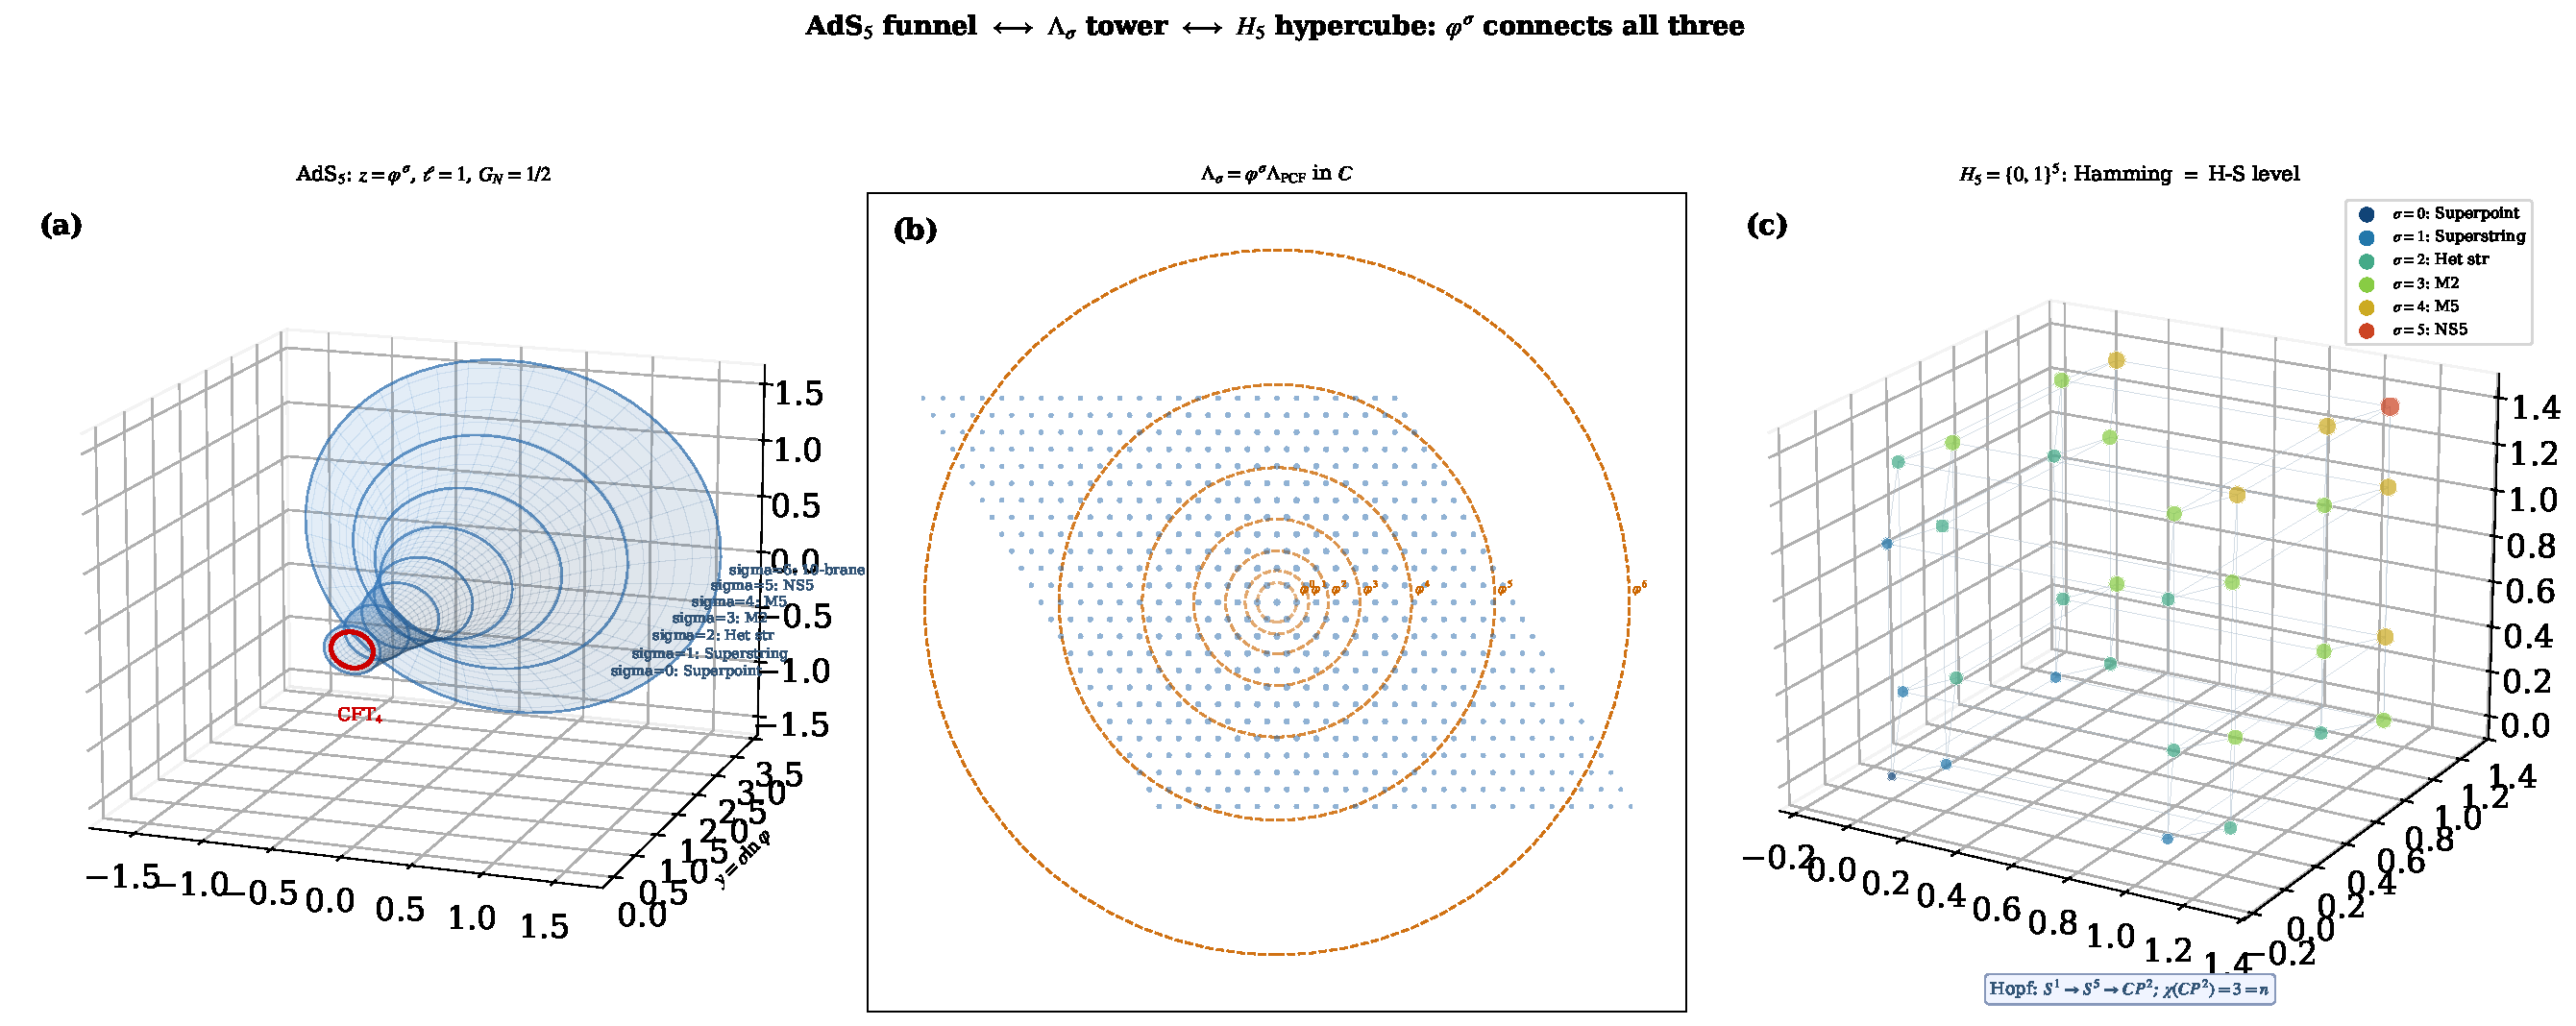
\includegraphics{fig5_three_panel.pdf}}
\caption{$\mathrm{AdS}_5$ funnel $z=\golden^{\sigma}$ \eqref{eq:throat} $\leftrightarrow$ the
lattice tower $\Lambda_\sigma$ $\leftrightarrow$ the Hamming hypercube $H_5$ of the M-theory
ladder (superpoint~$\to$~NS5); $\golden^{\sigma}$ connects all three:
(a) the funnel with $\ell=1$, $G_N=\tfrac12$; levels bottom-to-top are
superpoint ($\sigma{=}0$), superstring ($\sigma{=}1$), het string ($\sigma{=}2$),
M2-brane ($\sigma{=}3$), M5-brane ($\sigma{=}4$), NS5-brane ($\sigma{=}5$), 10-brane ($\sigma{=}6$);
(b) the Eisenstein lattice $\Lambda_\sigma=\golden^{\sigma}\Lambda_{\rm PCF}$ in $\C$ with concentric $\golden$-rings;
(c) the Hamming cube $H_5=\{0,1\}^5$ coloured by Hamming weight $=$ H-S level.}
\label{fig:ads-ladder}
\end{figure}
The bulk--boundary map is an isometry---proved here as Lemma~\ref{lem:isometry}, and independently in the companion~\cite{HP}---used in \S\ref{sec:dof}, and it obeys the GKPW dictionary~\cite{Maldacena98,GKP98,Witten98},
\begin{equation}\label{eq:isometry}
  V:\mathcal H_{\mathrm{bulk}}\to\mathcal H_{\partial},\qquad V^{\dagger}V=\mathbf 1,\qquad
  Z_{\mathrm{grav}}\big[\phi|_{\partial}\big]
   =\big\langle e^{\int_{\partial}\phi_{0}\mathcal O}\big\rangle_{\mathrm{CFT}}.
\end{equation}
\paragraph{The isometry as an algebra--isometry (bulk--boundary) duality.}
The embedding $V$ \eqref{eq:isometry} is realised on the two faces of one modulus. The eigenvalue
triangle $\lambda_k=\tfrac12\omega^{k}$ ($\omega=e^{2\pi i/3}$) of Prop.~\ref{prop:pcf-norms}
\eqref{eq:norms-derived} is the Eisenstein lattice $\Z[\omega]$ (\emph{algebra} face: $120^\circ$,
$S_3$ symmetry, $A_2$ root system $=\mathfrak{su}(3)$)
\ProofWitnessBlock{eisenstein\_omega, Omega\_eigenvalues, a2\_minimal\_vectors\_exactly\_six};
the same modulus on the
$i/\pi$ side, where $(\tfrac12)!=\tfrac12\sqrt\pi$ fixes $\mu=\tfrac12$ (\S\ref{ssec:construction}),
is the Gauss lattice $\Z[i]$ (\emph{isometry} face: $\tau=i$, $\ell=1$). The $\golden$-mediation
$S_3\to\Z_4$ between them preserves $|\Om|=\tfrac12$ \ProofWitness{holographic\_area} and fixes $\tau=i$:
this is $V^{\dagger}V=\mathbf 1$ read on the lattice --- bulk (geometry, $\Z[i]$) and boundary
(algebra, $\Z[\omega]$) are two readings of one triangle, neither privileged, exactly as
\eqref{eq:isometry} requires.  for the two lattices and the mediation; the GKPW dictionary \ProofWitness{holographic\_area, hopf\_from\_clifford, hopf\_latitude, G\_AB\_pcf, Lambda5\_pcf, R\_scalar\_pcf, BF\_value, Omega\_eigenvalues, a2\_minimal\_vectors\_exactly\_six, eisenstein\_omega, hypercube\_card, holographic\_area, hopf\_from\_clifford, hopf\_latitude, G\_AB\_pcf, Lambda5\_pcf, R\_scalar\_pcf, BF\_value, Omega\_eigenvalues, a2\_minimal\_vectors\_exactly\_six, eisenstein\_omega, hypercube\_card}
of \eqref{eq:isometry} enters cited, ~\cite{Maldacena98,GKP98,Witten98}. \HypWitness{\cite{Maldacena98, GKP98, Witten98}}
\begin{figure}[!htbp]\centering\n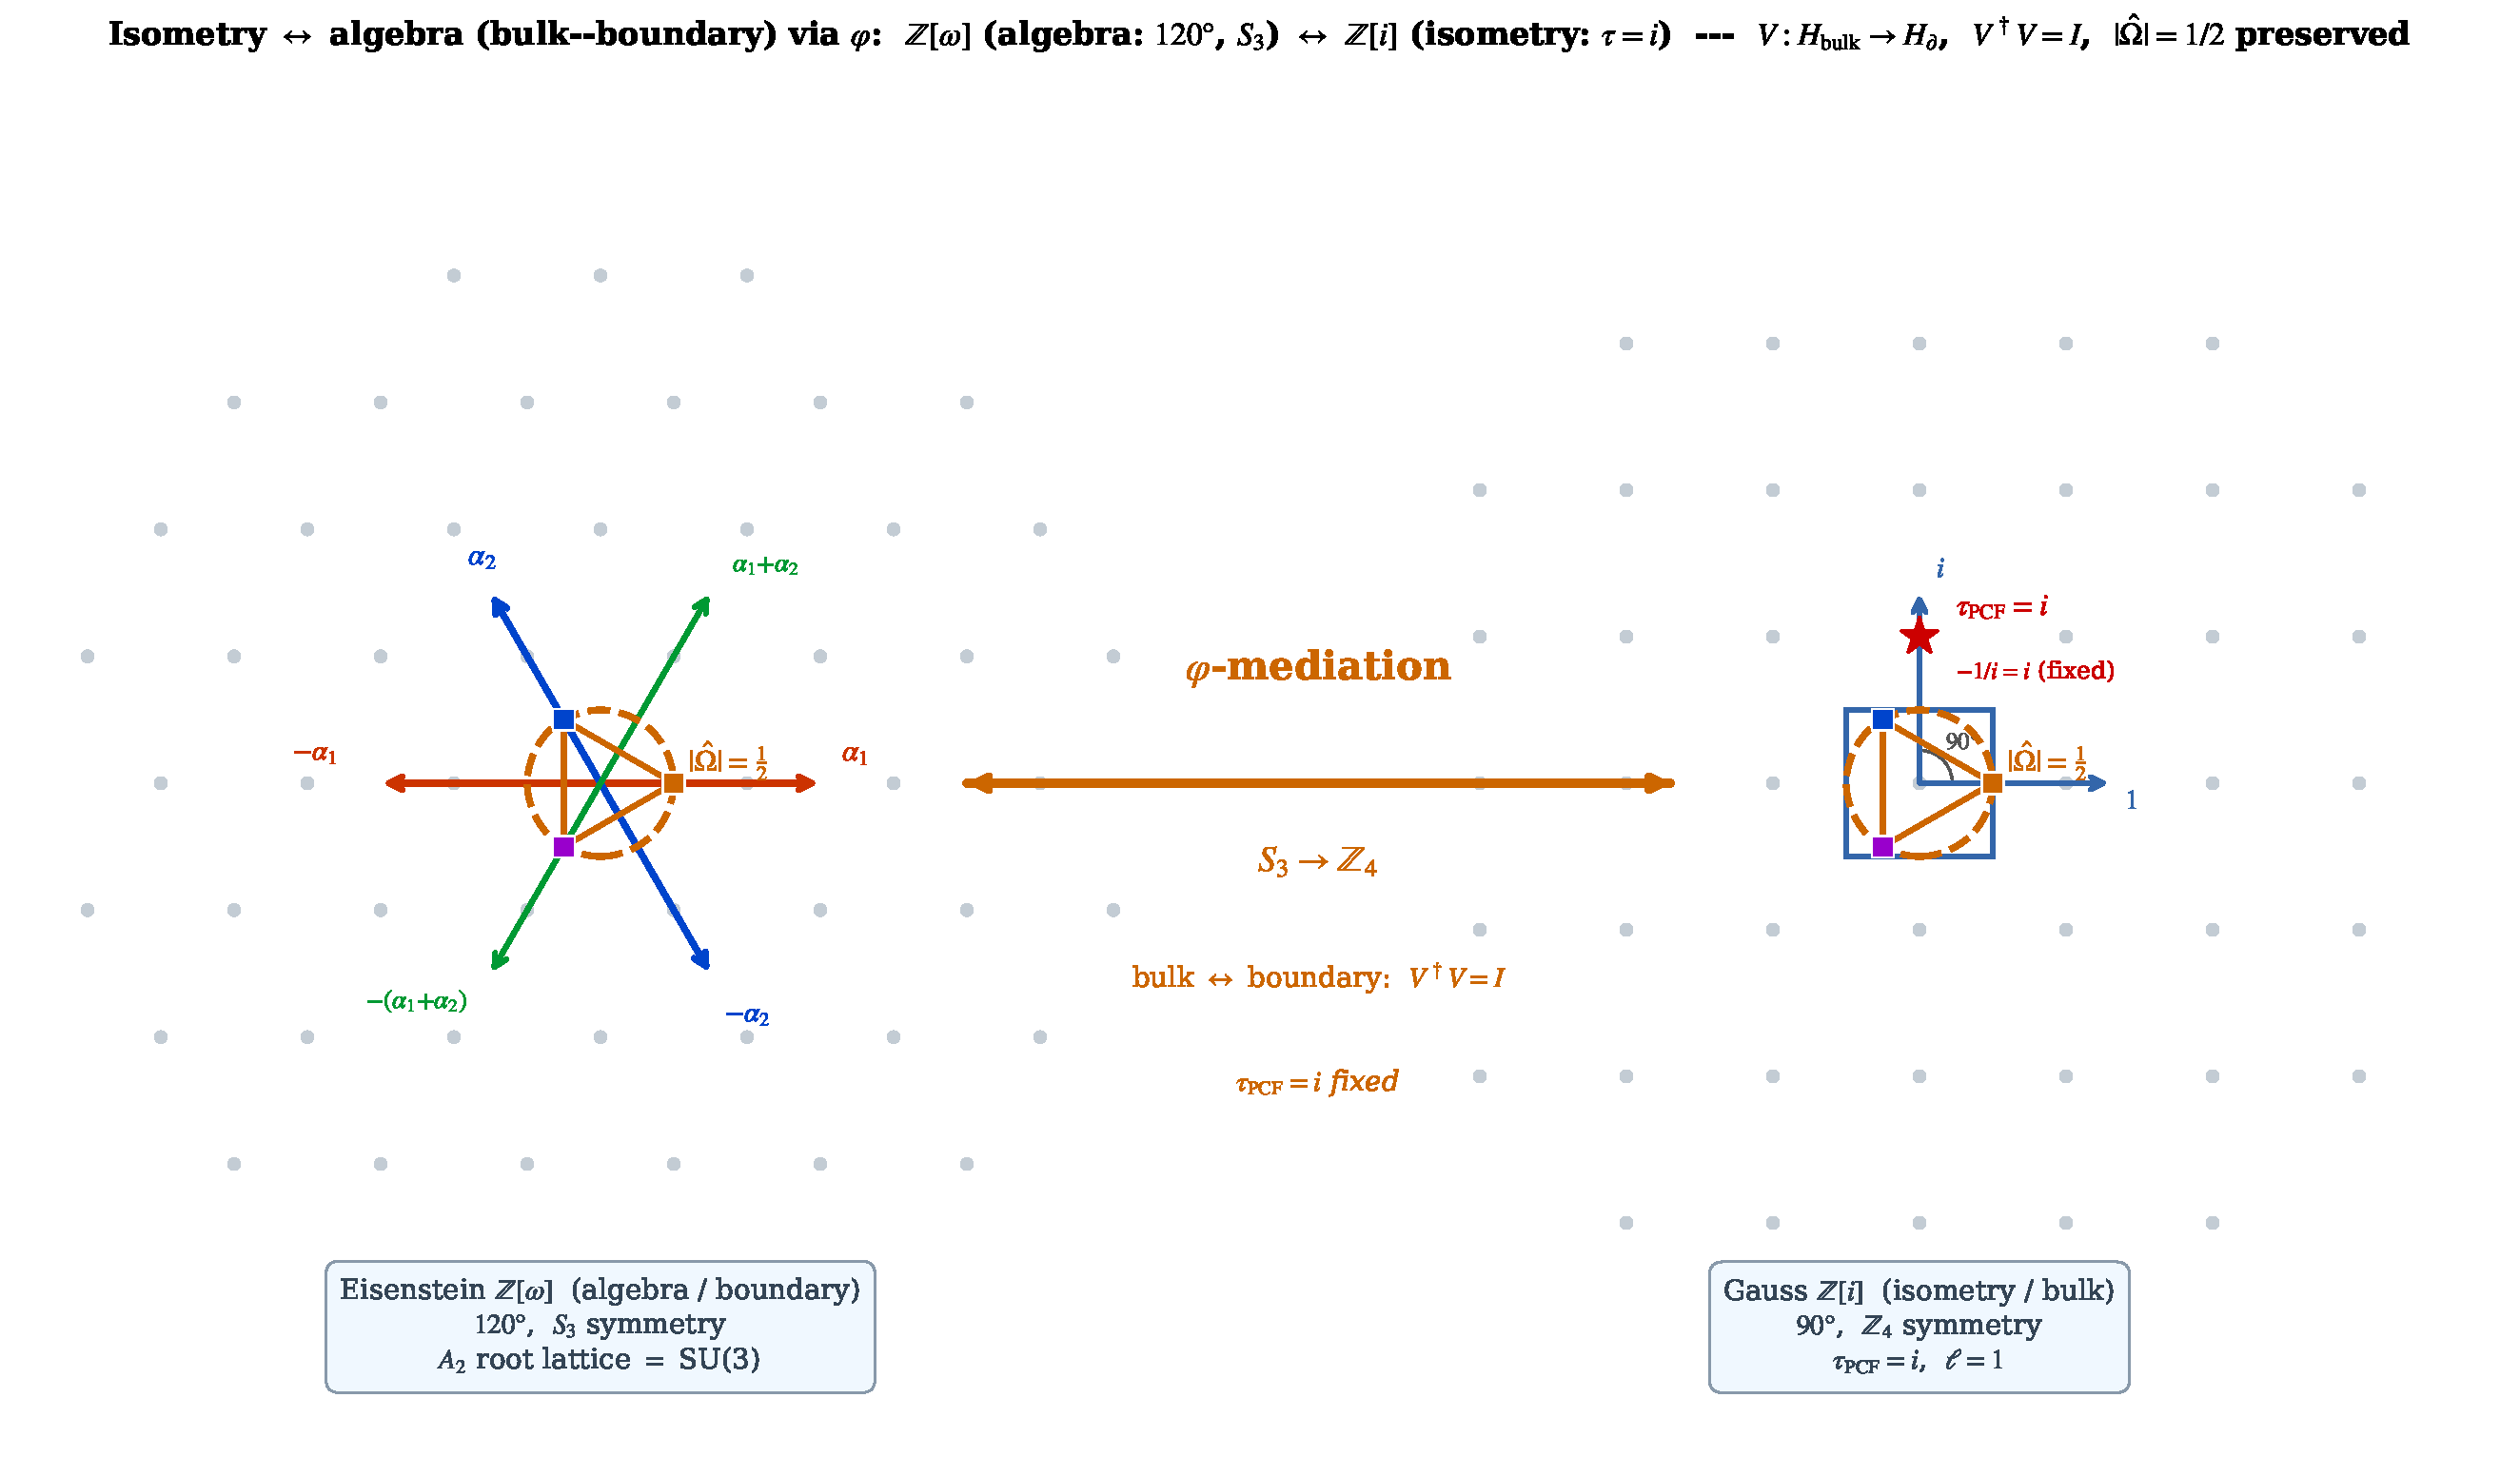
\includegraphics[width=\linewidth,trim={0 5cm 0 5cm},clip]{fig4_top_down.pdf}
\caption{Isometry $\leftrightarrow$ algebra (bulk--boundary): left, the Eisenstein lattice $\Z[\omega]$
($120^\circ$, $S_3$ symmetry, $A_2=\mathfrak{su}(3)$, algebra/boundary);
right, the Gauss lattice $\Z[i]$
($90^\circ$, $\Z_4$ symmetry, $\tau=i$, $\ell=1$, isometry/bulk).
They are $\golden$-mediated ($S_3\to\Z_4$) with $|\Om|=\tfrac12$ preserved --- the
lattice realisation of $V:\mathcal H_{\mathrm{bulk}}\to\mathcal H_{\partial}$,
$V^{\dagger}V=\mathbf 1$ \eqref{eq:isometry}.}
\label{fig:isometry-algebra}
\end{figure}
Standard AdS/CFT integrates out the radial coordinate $z$ (it privileges a boundary); here
the isometry singles out neither side, so PCF keeps both bulk and boundary
(\eqref{eq:isometry}; ``forget $z$'' only on the Maldacena side).
The modulus is scale invariant, so the holographic relation holds at every level:
\begin{equation}\label{eq:tower-autosimilar}
  |\Om|_{\sigma}=\tfrac12\qquad\forall\,\sigma .
\end{equation}
The self-similarity is the physical face of the Frobenius lift \eqref{eq:frobenius-tower}: both
act on the golden monoid through the one composition law $\psi_p(\golden^{\,n})=(\golden^{\,n})^{p}$,
exponents multiplying while the modulus stands.
The gravitational data follow from the same $\mu=\tfrac12$, the $\tfrac34$ of the signature being
the $\lVert v\rVert^{2}$ of \eqref{eq:isometry-triad} read as the colour ratio
(Remark~\ref{rmk:spectral-origin}): \ProofWitness{bulkBoundary\_isometry, spectral\_uniqueness, bulkBoundary\_isometry}
\begin{equation}\label{eq:brown-henneaux}
  \SBH=\frac{1}{4\GN}=\mu=\tfrac12,\qquad c=\frac{3\ell}{2\GN}=3\quad(\ell=1,\ \GN=\tfrac12).
\end{equation}
This closes the circle to \S\ref{ssec:object}: the Newton constant is the worldline modulus
itself, $\GN=|\Om(\tau)|$ for every $\tau$ \eqref{eq:worldline}, and the central charge singles
that value out---$3\ell/(2G)=3$ iff $G=\tfrac12$.

\begin{remark}[The role of $\golden$ in AdS/CFT]
\sloppy Everything follows from the microstate $\Om$ (\S\ref{ssec:object}) and the tower
(\S\ref{ssec:p-tower}); the modulus is $\mu=\tfrac12$ at every level, and the AdS/CFT
signature $(\ell{=}1,\GN{=}\tfrac12,c{=}3,\mathrm{GKP}{=}\tfrac34)$ is exactly the microstate's
invariants.
\end{remark}

\paragraph{Thread (all AdS/CFT from one microstate).}
\begin{enumerate}
  \item the isometry $V$ with $V^{\dagger}V=\mathbf 1$ embeds bulk into boundary preserving the norm,
        so the duality holds from \emph{one} state, without averaging
        (\eqref{eq:worldline}$\to$\eqref{eq:isometry});
  \item the modulus is scale invariant, $|\Om|_{\sigma}=\tfrac12\ \forall\sigma$, so the holographic
        relation holds at \emph{each} level of the throat, not only at the boundary
        \eqref{eq:tower-autosimilar};
  \item from the same $\mu=\tfrac12$: $\SBH=1/(4\GN)=\tfrac12$ (area law) and $c=3$ (Brown--Henneaux)
        --- the gravity-side entropy and central charge come from the microstate invariant
        \eqref{eq:brown-henneaux};
  \item hence GKPW~\cite{GKP98,Witten98} and Ryu--Takayanagi~\cite{RyuTakayanagi06} are consequences of the isometric embedding of the microstate.
\end{enumerate}
Thus the entire AdS/CFT correspondence comes from one microstate, not an ensemble. (Numerically verified: $|\Om|_{\sigma}=\tfrac12\ \forall\sigma$ via \eqref{eq:certainty},
$\mathrm{GKP}=\tfrac34$, $\SBH=\mu$, $c=3$.)

Maldacena left the AdS boundary conditions unspecified---``we leave this interesting problem
for the future''~\cite{Maldacena98}. Here they are determined: the modular parameter is fixed
at $\tau=i$, the fixed point of S-duality
and the scale by the
certainty principle $\varepsilon_0 M_{\PCF}=\pi$.
\ProofWitnessBlock{certainty\_principle}

% --- 3.5 ---

\subsection{The M-theory type duality web from the microstate}\label{ssec:web}
The M-theory type duality web projects from the microstate (\S\ref{ssec:object}) through the
$\golden^{\sigma}$ tower (\S\ref{ssec:p-tower}); Witten's eight/eleven-dimensional object is not
required here. Witten \emph{posits} that object and \emph{conjectures} that the web follows from it
\cite{Witten95}; PCF starts from a \emph{demonstrated} microstate and \emph{generates} the tower, of
which the web is a projection. The web follows from the tower with HS (\S\ref{ssec:p-tower}) and from
per-level AdS/CFT (\S\ref{ssec:adscft}), both already stated. The shared signature, derived in
App.~\ref{app:web} from the web's two corners, is that the M-theory object and AdS/CFT are
projections of the microstate, carrying
\begin{equation}\label{eq:shared-signature}
  \underbrace{|\Om|=\tfrac12,\ |\Om|^{2}=\tfrac14}_{\text{Huerta--Schreiber (M-theory)}}\qquad
  \underbrace{\ell=1,\ \GN=\tfrac12,\ c=3,\ \mathrm{GKP}=\tfrac34}_{\text{Maldacena (AdS/CFT)}} ,
\end{equation}
which equal the microstate invariants $\mu=\tfrac12$. That the two corners are one and the
same object is Maldacena's conjecture that ``M/string theory on various Anti-deSitter
spacetimes is dual to various conformal field theories''~\cite{Maldacena98}---the definition of
M-theory he anticipated extending to five non-compact dimensions: here it is realised, both corners being
projections of the single microstate $|\Om|=\tfrac12$. The torus on which they meet is the
noncommutative torus that Connes, Douglas and Schwarz identify with M-theory
compactification~\cite{connes98} and that Manin attaches to the $\F_1$ program~\cite{manin04};
the non-orientable fibre it carries is independent of that algebra (Prop.~\ref{prop:mobius-torus}). The dualities that engage the tower are
\begin{align}
  \text{(S-duality)}\quad & \tau\to-\tfrac1\tau\ \Longleftrightarrow\ \golden\to-\tfrac1\golden
    =\bar\golden, \label{eq:bridge-S}\\
  \text{(T-duality)}\quad & R\to\alpha'/R, \label{eq:bridge-T}\\
  \text{(IIA strong coupling)}\quad & \sigma=10\to\sigma=11\ \ (\text{M-theory}), \label{eq:bridge-Witten}\\
  \text{(ER}=\text{EPR)}\quad & \text{entanglement}\leftrightarrow\text{geometry}, \label{eq:bridge-ER}\\
  \text{(de Sitter swampland)}\quad & \frac{|\partial_{\sigma}V|}{V}=\ln\golden, \label{eq:dS-swampland}\\
  \text{(asymptotic safety)}\quad & \text{UV fixed point}.\ProofWitness{c\_tendsto\_two} \label{eq:bridge-fixed}
\end{align}

\begin{remark}[S-duality is the involution of \S\ref{ssec:zeta}]\label{rmk:S-is-involution}
The S-duality \eqref{eq:bridge-S} is, in the Schwinger variable, the involution $t\mapsto1/t$ under
which the Gaussian lattice sum transforms with weight $\tfrac12$,
$\Theta(1/t)=\sqrt t\,\Theta(t)$ \eqref{eq:theta-lattice}, and whose unique fixed point $t=1$ is
$\tau=i$ (Proposition~\ref{prop:archimedean}). What \S\ref{ssec:zeta} proves is the transformation;
what \eqref{eq:bridge-S} adds is that the string's electric--magnetic duality and the Galois
conjugation $\golden\to-1/\golden$ are that same involution read on the coupling and on the field.
\ProofWitnessBlock{theta\_from\_jacobi, theta\_fixed\_point\_unique}
\end{remark}


\begin{remark}[The IIA$\to$11D bridge as Witten's Kaluza--Klein tower]
The bridge $\sigma=10\to\sigma=11$ in \eqref{eq:bridge-Witten} corresponds to Witten's Kaluza--Klein
mechanism: at Type~IIA strong coupling the tower of states are the Kaluza--Klein modes of
eleven-dimensional supergravity on $\R^{10}\times S^1$, of mass $\sim 1/r$~\cite{Witten95}. The
$\golden^{\sigma}$ tower plays that role here. The golden Kaluza--Klein structure
($\golden^2+\golden^{-2}-2=1$; $G_5\to G_4=\tfrac14$; the Breitenlohner--Freedman comparison;
discrete-spectrum stability) is proved in Appendix~\ref{app:kk}.
\end{remark}

\begin{remark}[The role of $\golden$ in the duality web]
The dualities are projections of the microstate's $\golden^{\sigma}$ tower, not of a posited object;
the modulus is $\mu=\tfrac12$ at every level, and S-duality is the Galois conjugation
$\golden\to-1/\golden$.
\end{remark}

\begin{remark}[the web is reconstructed from its two corners]
The web this paper uses has two corners only---Huerta--Schreiber M-theory and Maldacena AdS/CFT---and both
are shown in Appendix~\ref{app:web} to carry the microstate modulus $|\Om|=\tfrac12$; the dualities are the
symmetries of the $\golden^{\sigma}$ tower that fix it. The wider string-theory content (U-duality, $E_8$, the
five string theories) is neither used nor needed here.
\end{remark}

\paragraph{Thread (microstate $\to$ tower $\to$ web).}
\begin{enumerate}
  \item the dualities are written in $\sigma/\golden$, as projections of the tower: S as
        $\golden\to-1/\golden$ (Galois conjugate), T as $R\to\alpha'/R$, IIA$\to$11D as $\sigma=10\to11$,
        ER$=$EPR, and the de Sitter swampland $|\partial_{\sigma}V|/V=\ln\golden$
        (\eqref{eq:bridge-S}--\eqref{eq:dS-swampland});
  \item the shared signature \eqref{eq:shared-signature}: the \emph{framework colimit} proves the
        M-theory object
        (modulus $\tfrac12$) and AdS/CFT ($\ell{=}1,\GN{=}\tfrac12,c{=}3,\mathrm{GKP}{=}\tfrac34$) are
        projections with the microstate invariants ($\mu=\tfrac12$)---this is the colimit of
        \emph{frameworks}, not the Euler colimit of \S\ref{ssec:tower};
  \item hence the web is reconstructed from its two corners (App.~\ref{app:web}): both carry $\mu=\tfrac12$, and
        the dualities fix the modulus; Witten's eight-dimensional object is not required.
\end{enumerate}
Thus microstate $\to$ tower $\to$ web (HS and per-level AdS/CFT). The quantitative pieces
($\golden\to-1/\golden$, the swampland constant $\ln\golden$ (the regulator $R_K$,
Definition~\ref{def:regulator}), the T-self-dual radius, and the
shared HS/Maldacena signature) are checked numerically (\eqref{eq:obs-swampland}, \eqref{eq:obs-jacobson})
and formally in \texttt{CW6\_complete\_v2.lean} (\S\ref{ssec:status}); the framework colimit
itself---the five frameworks and the PCF core as partial spectral objects, the cocone into the
vertex $T_{\PCF}$, and its universal property---is proved in the same file
(\texttt{cocone\_property}, \texttt{colimit\_universal}, \texttt{framework\_colimit}).


The remaining duality, $\mathrm{ER}=\mathrm{EPR}$, is where the microstate supplies what
Cool Horizons left open. Maldacena and Susskind observe that the ER bridge ``may be a highly
quantum object that is yet to be independently defined'', and that they ``do not have an
independent argument for its smoothness''~\cite{MaldacenaSusskind13}. In PCF the bridge is
both defined and analytic: it is the cocycle $T(\sigma_1,\sigma_2)$ of the proposition below,
smooth in the analytic sense because its denominator $1+\varepsilon_0\golden^{\sigma}$ is strictly positive at
every level, carried, with its geometry supplied by the non-orientable fibre, on the M-theory
noncommutative torus rather than on a general quantum object.

% ====== BLOQUE MOVIDO desde §4.4 (era L1785–1825): prop:er-epr + fig + proof ======
\begin{proposition}[$\mathrm{ER}=\mathrm{EPR}$ from the modulus]\label{prop:er-epr}
The entanglement of the two hemispheres and the geometric bridge between them are one
invariant, $\mu_3^{2}=\tfrac14$.
\emph{(EPR.)} Since $|\Om(\tau)|=\tfrac12$ for every $\tau$ \eqref{eq:worldline}, the two-point
entanglement modulus is
\[
  |\Om(\tau_A)\,\overline{\Om(\tau_B)}|=|\Om(\tau_A)|\,|\Om(\tau_B)|=\mu_3^{2}=\tfrac14
  \qquad(\forall\,\tau_A,\tau_B),
\]
which is the holographic area factor $\mu_3^{2}=\tfrac14$. % FIX: era \eqref{eq:obs-cramerrao} (§4), ahora directo (autocontenido en §3)
\emph{(ER.)} The bridge amplitude between two levels of the throat,
$T(\sigma_1,\sigma_2)=\dfrac{1+\epsz\golden^{\sigma_1}}{1+\epsz\golden^{\sigma_2}}$,
satisfies $T(\sigma_1,\sigma_2)\,T(\sigma_2,\sigma_1)=1$ and
$T(\sigma_1,\sigma_2)\,T(\sigma_2,\sigma_3)=T(\sigma_1,\sigma_3)$, so the bridges form a group:
a round trip is the identity and composition is additive in $\sigma$.
\emph{($\mathrm{ER}=\mathrm{EPR}$.)} Both are fixed by the one scale-independent modulus
$\mu_3=\tfrac12$ ($|\Om|_\sigma=\tfrac12\ \forall\sigma$, \eqref{eq:tower-autosimilar}): the
entanglement between $P$ (south) and $F$ (north), mediated by $C$, \emph{is} the bridge that joins
them through the equatorial axis. Entanglement is geometry, derived from the modulus, not posited.
\ProofWitnessBlock{bridge\_cocycle, bridge\_inverse, bridge\_compose} % ADD fase 1: respaldo Lean del cociclo
\end{proposition} The bridge and its $\tfrac14$ identity are shown in Fig.~\ref{fig:er-epr}.

\begin{proof}
\emph{(EPR)} $\Om(\tau)=\tfrac12 e^{\,i\tau\ln\golden}$ has $|\Om(\tau)|=\tfrac12=\mu_3$ for all
$\tau$ \eqref{eq:worldline}; the product rule for moduli gives
$|\Om(\tau_A)\overline{\Om(\tau_B)}|=\mu_3^{2}=\tfrac14$, independent of $\tau_A,\tau_B$ because
$\mu_3$ comes from the $S_3$ arity (Proposition~\ref{prop:pcf-norms}), not from the phase.
\emph{(ER)} $T(\sigma_2,\sigma_1)$ is the reciprocal of $T(\sigma_1,\sigma_2)$, whence
$T(\sigma_1,\sigma_2)T(\sigma_2,\sigma_1)=1$; the telescoping of numerator and denominator gives
$T(\sigma_1,\sigma_2)T(\sigma_2,\sigma_3)=T(\sigma_1,\sigma_3)$.
\emph{($\mathrm{ER}=\mathrm{EPR}$)} The levels are equivalent because
$\epsz\golden^{\sigma}\!\cdot\!\Mpcf\golden^{-\sigma}=\pi$ at every $\sigma$ \eqref{eq:certainty}, so
$|\Om|_\sigma=\tfrac12$ is scale-invariant \eqref{eq:tower-autosimilar}; the entanglement invariant
$\mu_3^{2}$ and the bridge group thus share one origin.
\end{proof}

\begin{figure}[!htbp]\centering\n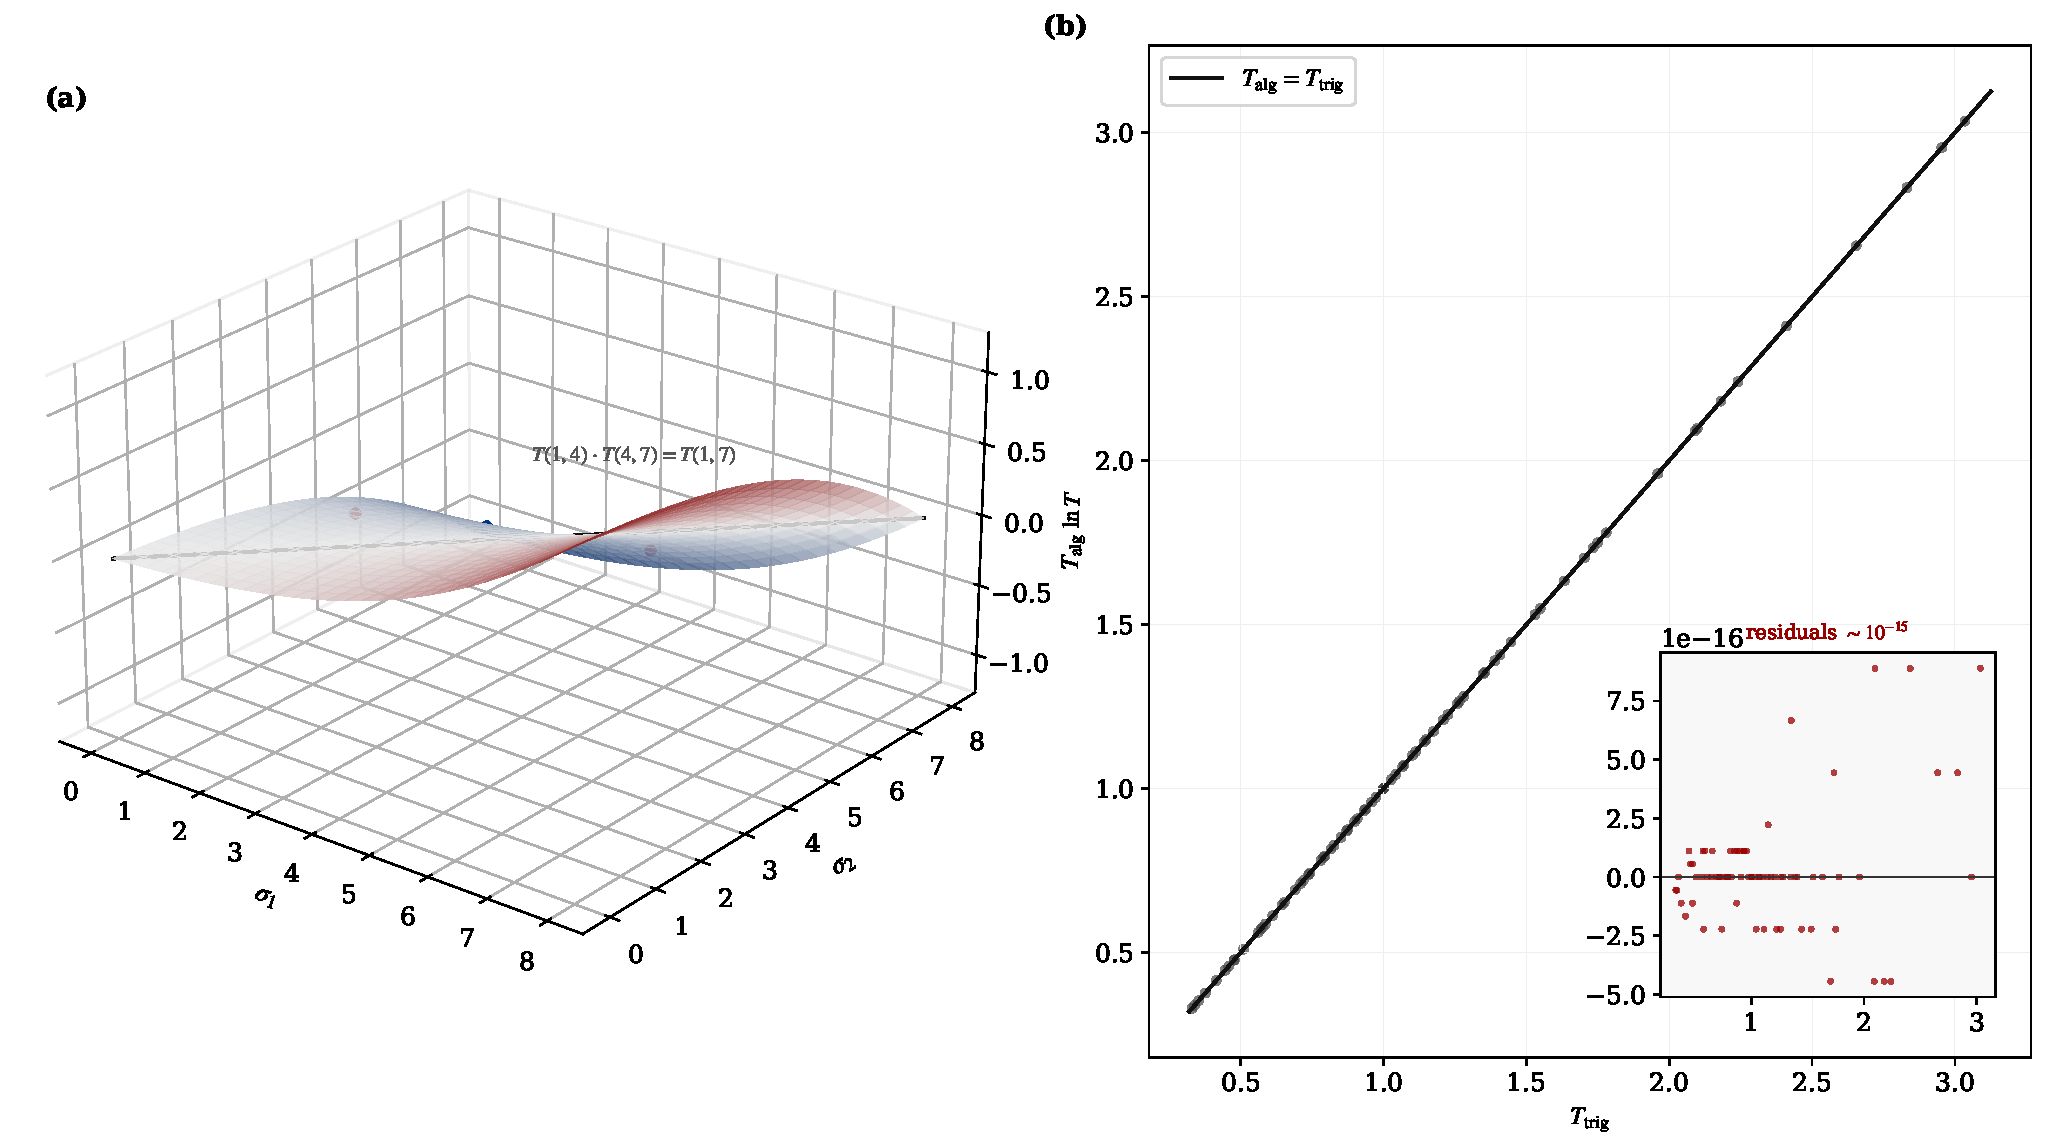
\includegraphics[width=\linewidth]{fig2_ER_bridge_identity.pdf}
\caption{$\mathrm{ER}=\mathrm{EPR}$ from the modulus (Prop.~\ref{prop:er-epr}): (a) the bridge
amplitude $T(\sigma_1,\sigma_2)$ as a cocycle, $T(1,4)\,T(4,7)=T(1,7)$; (b) the algebraic and
trigonometric forms agree, $T_{\mathrm{alg}}=T_{\mathrm{trig}}$, to machine precision --- which is
Corollary~\ref{cor:bridge-angle}, \eqref{eq:bridge-angle}, and not a numerical accident.}
\label{fig:er-epr}
\end{figure}

\begin{corollary}[The bridge is the spectral angle]\label{cor:bridge-angle}
With $\alpha(\sigma)$ of Proposition~\ref{prop:spectral-angle-tower},
\begin{equation}\label{eq:bridge-angle}
  T(\sigma_1,\sigma_2)
  =\frac{1+\tan\alpha(\sigma_1)}{1+\tan\alpha(\sigma_2)}
  =\frac{\sin\bigl(\alpha(\sigma_1)+\tfrac\pi4\bigr)\,\cos\alpha(\sigma_2)}
        {\sin\bigl(\alpha(\sigma_2)+\tfrac\pi4\bigr)\,\cos\alpha(\sigma_1)} .
\end{equation}
The first equality is \eqref{eq:spectral-angle}; the second is
$\sqrt2\,\sin(\alpha+\tfrac\pi4)/\cos\alpha=1+\tan\alpha$, and the $\tfrac\pi4$ enters for one
reason only: $\tan\tfrac\pi4=1$ is the $1$ that the cocycle adds to $\epsz\golden^{\sigma}$. So the
$\mathrm{ER}=\mathrm{EPR}$ bridge and the spectral angle are one object, and the trigonometric form
that Fig.~\ref{fig:er-epr} plots against the algebraic one is an identity, not a numerical
coincidence. \ProofWitness{bridge\_eq\_tan\_form, bridge\_pi\_quarter, spectral\_angle\_tan}

\end{corollary}
\begin{proof}
$\sin(\alpha+\tfrac\pi4)=(\sin\alpha+\cos\alpha)/\sqrt2$, so
$\sqrt2\sin(\alpha+\tfrac\pi4)/\cos\alpha=1+\tan\alpha$ whenever $\cos\alpha\neq0$, which holds
since $\alpha(\sigma)<\pi/2$. Forming the quotient at $\sigma_1$ and $\sigma_2$ cancels the
$\sqrt2$, and $\tan\alpha(\sigma_i)=\epsz\golden^{\sigma_i}$ returns the algebraic form of
Proposition~\ref{prop:er-epr}.
\end{proof}
% ====== fin del bloque movido ======

\begin{proposition}[Two towers, one microstate]\label{prop:two-towers}
Carrying boundary degrees of freedom into the bulk requires, in the standard treatments, a tower:
the Virasoro algebra with its central charge on the holographic side, and the chain of maximal
invariant central extensions of the superpoint, $\R^{0|1}\to\cdots\to\R^{10,1|32}$, on the M-theory
side (\S\ref{app:superpoint} below). Each is built independently and each is costly; covering what they
must cover takes a great deal of structure. Neither is contradicted here. What the colimit
\eqref{eq:shared-signature} adds is that they are two routes to one vertex, and this is visible in
four places at once.

First, \emph{strings and holography commute in $c$}. The central charge arrives twice---from the
worldsheet \eqref{eq:polyakov} and from Brown--Henneaux $c=3\ell/(2\GN)$ with the derived $\ell=1$
and $\GN=\tfrac12=|\Om|$ \eqref{eq:brown-henneaux}---and the two arrivals are the same component of
the vertex, not two values that agree. The one free parameter of the Virasoro tower is therefore the
microstate modulus: $3\ell/(2\GN)=3$ holds only at $\GN=\tfrac12$.

Second, \emph{the ladder is counted by the turn}. Its $32$ supercharges are $|H_5|=2^{5}$, and the
$2$ that counts them satisfies in $\F_5$ the equation the turn satisfies in $\C$
\eqref{eq:two-is-i}: the binary side of the ladder and the $\C$ level of the dimensional chain
\eqref{eq:dim-chain} are one generator, reduced. Field theory and group theory meet at the same
place: the two quadratic fields $\Q(i)$ and $\Q(\sqrt5)$ have coprime conductors $4$ and $5$, and
their product $20$ carries a character group whose two factors govern one character each and no more
\eqref{eq:attribution}.

Third, \emph{one recurrence covers the ladder}. The tower advances by $S(\sigma+1)=\golden S(\sigma)$
and the bulk--boundary ratio is $\pi/m_0$ at every level (\eqref{eq:intertwine} below); in any other base the
ratio would drift and no level-wise isometry could intertwine them. With no level privileged, the
many discrete steps are an index on one flow rather than a stack of separate structures---which is
why $\sigma=10\to11$ \eqref{eq:bridge-Witten} is one more level and not one more theory.

Fourth, \emph{dimension three is reached by an isometry, not by an algebra}. Frobenius's theorem
leaves only $1,2,4$ for a finite-dimensional associative real division algebra, and $3$ is not among
them~\cite{Frobenius1878}; yet the chain \eqref{eq:dim-chain} reaches $\E^{3}$. There is no
contradiction because no product in dimension three is ever asked for: what reaches it is the
norm-preserving---hence injective, hence faithful---embedding $V\colon\C\to\C^{3}$ of
Lemma~\ref{lem:isometry}. The algebraic bound and the geometric reach are different questions, and
the isometry is what carries one to the other, as the Frobenius lift \eqref{eq:frobenius-tower}
carries the same modulus on the arithmetic side.

Taken together: the complexity each tower needs on its own is the cost of not having the microstate.
for the four items; the Virasoro and brane-bouquet constructions themselves enter cited, \ProofWitness{psi\_functorial, psi\_one}
~\cite{BrownHenneaux86,Witten95}. \HypWitness{\cite{BrownHenneaux86, Witten95}}
\end{proposition}

\subsection{The demonstrative line (20-step spine, seeded by \S\ref{sec:methods})}\label{ssec:spine}
\begin{figure}[htb]\centering
\resizebox{\textwidth}{!}{%
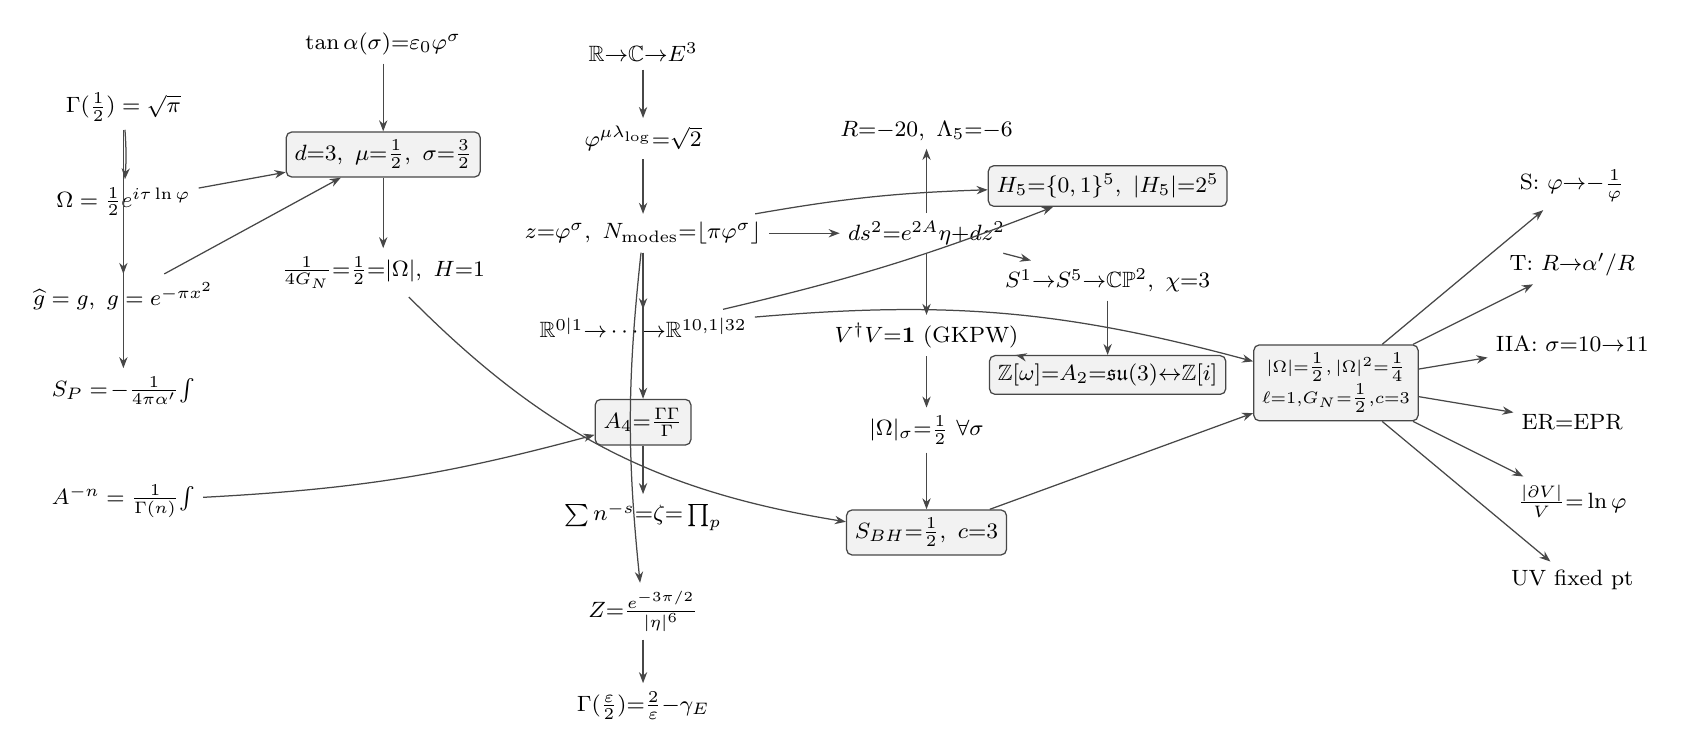
\begin{tikzpicture}[
  font=\footnotesize,
  >={Stealth[length=4pt]},
  nd/.style={inner sep=2pt, outer sep=1pt},
  ap/.style={draw, rounded corners=2pt, fill=black!5, inner sep=3pt},
  every path/.style={->, draw=black!72, line width=0.45pt}]

% ===== 3.1 object (x=0) =====
\node[nd] (gh) at (0,5.6)  {$\Gamma(\tfrac12)=\sqrt\pi$};
\node[nd] (wl) at (0,4.4)  {$\Om=\tfrac12 e^{i\tau\ln\golden}$};
\node[nd] (gs) at (0,3.2)  {$\widehat g=g,\ g=e^{-\pi x^{2}}$};
\node[nd] (pk) at (0,2.0)  {$S_P=\!-\tfrac{1}{4\pi\alpha'}\!\int$};
\node[nd] (sw) at (0,0.6)  {$A^{-n}=\tfrac{1}{\Gamma(n)}\!\int$};

% ===== 3.2 meta (x=3.3) =====
\node[ap] (si) at (3.3,5.0) {$d{=}3,\ \mu{=}\tfrac12,\ \sigma{=}\tfrac32$};
\node[nd] (al) at (3.3,6.4) {$\tan\alpha(\sigma){=}\epsz\golden^\sigma$};
\node[nd] (bh) at (3.3,3.5) {$\tfrac{1}{4\GN}{=}\tfrac12{=}|\Om|,\ H{=}1$};

% ===== 3.3 tower + amplitudes (x=6.6) =====
\node[nd] (dc)  at (6.6,6.3)  {$\R{\to}\C{\to}E^3$};
\node[nd] (tm)  at (6.6,5.2)  {$\golden^{\mu\lng}{=}\sqrt2$};
\node[nd] (tmo) at (6.6,4.0)  {$z{=}\golden^\sigma,\ \Nmodes{=}\lfloor\pi\golden^\sigma\rfloor$};
\node[nd] (hs)  at (6.6,2.8)  {$\R^{0|1}{\to}\cdots{\to}\R^{10,1|32}$};
\node[ap] (vz)  at (6.6,1.6)  {$A_4{=}\tfrac{\Gamma\Gamma}{\Gamma}$};
\node[nd] (re)  at (6.6,0.4)  {$\sum n^{-s}{=}\zeta{=}\prod_p$};
\node[nd] (pp)  at (6.6,-0.8) {$Z{=}\tfrac{e^{-3\pi/2}}{|\eta|^{6}}$};
\node[nd] (gp)  at (6.6,-2.0) {$\Gamma(\tfrac\varepsilon2){=}\tfrac2\varepsilon{-}\gamma_E$};

% ===== 3.4 AdS/CFT (x=10.2) =====
\node[nd] (th)  at (10.2,4.0) {$ds^2{=}e^{2A}\eta{+}dz^2$};
\node[nd] (iso) at (10.2,2.7) {$V^\dagger V{=}\mathbf1$ (GKPW)};
\node[nd] (ta)  at (10.2,1.5) {$|\Om|_\sigma{=}\tfrac12\ \forall\sigma$};
\node[ap] (bhn) at (10.2,0.2) {$S_{BH}{=}\tfrac12,\ c{=}3$};
\node[nd] (adsR) at (10.2,5.3) {$R{=}{-}20,\ \Lambda_5{=}{-}6$};
\node[ap] (h5)   at (12.5,4.6) {$H_5{=}\{0,1\}^5,\ |H_5|{=}2^5$};
\node[nd] (s5)   at (12.5,3.4) {$S^1{\to}S^5{\to}\mathbb{CP}^2,\ \chi{=}3$};
\node[ap] (lat)  at (12.5,2.2) {$\mathbb{Z}[\omega]{=}A_2{=}\mathfrak{su}(3){\leftrightarrow}\mathbb{Z}[i]$};

% ===== 3.5 web (x=13.7) =====
\node[ap] (ss)  at (15.4,2.1) {$\substack{|\Om|{=}\tfrac12,\,|\Om|^2{=}\tfrac14\\ \ell{=}1,\GN{=}\tfrac12,c{=}3}$};
\node[nd] (bS)  at (18.4,4.6) {S: $\golden{\to}{-}\tfrac1\golden$};
\node[nd] (bT)  at (18.4,3.6) {T: $R{\to}\alpha'/R$};
\node[nd] (bW)  at (18.4,2.6) {IIA: $\sigma{=}10{\to}11$};
\node[nd] (bER) at (18.4,1.6) {ER$=$EPR};
\node[nd] (bsw) at (18.4,0.6) {$\tfrac{|\partial V|}{V}{=}\ln\golden$};
\node[nd] (bfx) at (18.4,-0.4){UV fixed pt};

% ===== edges =====
\draw (gh) -- (gs);
\draw (gh) to[bend left=4] (wl);
\draw (wl) -- (pk);
\draw (wl) -- (si);
\draw (gs) -- (si);
\draw (sw) to[bend right=6] (vz);
\draw (si) -- (bh);
\draw (dc) -- (tm);
\draw (tm) -- (tmo);
\draw (tmo) -- (hs);
\draw (tmo) -- (vz);
\draw (tmo) to[bend right=6] (pp);
\draw (tmo) -- (th);
\draw (vz) -- (re);
\draw (pp) -- (gp);
\draw (th) -- (iso);
\draw (al) -- (si);
\draw (th) -- (adsR);
\draw (hs) to[bend right=4] (h5);
\draw (tmo) to[bend left=4] (h5);
\draw (th) -- (s5);
\draw (iso) -- (lat);
\draw (s5) -- (lat);
\draw (iso) -- (ta);
\draw (ta) -- (bhn);
\draw (bh) to[bend right=18] (bhn);
\draw (bhn) -- (ss);
\draw (hs) to[bend left=10] (ss);
\draw (ss) -- (bS);
\draw (ss) -- (bT);
\draw (ss) -- (bW);
\draw (ss) -- (bER);
\draw (ss) -- (bsw);
\draw (ss) -- (bfx);

\end{tikzpicture}
}
\caption{Commutative spine of \S\ref{sec:derivations} (P1$\to$P20): the thirty-one nodes carrying the twenty steps, arranged by subsection (the object, \S\ref{ssec:object}; the meta-invariant, \S\ref{ssec:meta}; the tower and amplitudes, \S\ref{ssec:p-tower}; AdS/CFT per level, \S\ref{ssec:adscft}; the duality web, \S\ref{ssec:web}), with the thirty-four demonstrative arrows. Shaded nodes are the six apices, where two or more independent chains converge on the same value; the forced invariants $d{=}3,\mu{=}\tfrac12,\sigma{=}\tfrac32$, with three incoming routes, are the maximal one. Seeded by the arithmetic of $K=\Q(\sqrt5)$ in \S\ref{sec:methods}; mathematical, physical and conceptual layers coincide on one diagram.}
\label{fig:spine3}
\end{figure}
Each step uses only previous steps.

\begin{description}
  \item[\S2$\to$\S3.] P1 $\Gamma(\tfrac12)=\sqrt\pi$ \eqref{eq:gamma-half} (\S\ref{ssec:origins}; seed)
        $\to$ P2 the self-dual Gaussian \eqref{eq:selfdual-gaussian}, its Mellin the Archimedean
        factor \eqref{eq:gammaR-mellin} and its lattice sum completing $\zeta$ into
        $\xi$ \eqref{eq:places-product} (\S\ref{ssec:zeta}).
  \item[3.1 object.] P3 $\Om,|\Om|=\tfrac12$ \eqref{eq:worldline}~(\S\ref{ssec:construction}) $\to$ P4 Gaussian, $\mu=\tfrac12$
        \eqref{eq:gaussian}~(\S\ref{ssec:origins}; width fixed by Prop.~\ref{prop:selfdual-gaussian}) $\to$ P5 worldsheet/Polyakov \eqref{eq:polyakov}.
  \item[3.2 meta-invariant.] P6 invariants $d{=}3,\mu{=}\tfrac12,\sigma{=}\tfrac32$
        \eqref{eq:spectral-invariants}~(\S\ref{ssec:arity},\,\S\ref{ssec:commute}) $\to$ P7 $1/(4\GN)=\tfrac12=|\Om|$, $H(\tfrac12)=1$
        \eqref{eq:bridge-BH}~(\S\ref{ssec:construction}).
  \item[3.3 tower $+$ HS.] P8 chain $i\to\golden$ \eqref{eq:dim-chain}~(\S\ref{ssec:spectrum}) $\to$ P9 $\sqrt2/\sqrt3$ by $\mu$
        \eqref{eq:tower-mediation}~(\S\ref{ssec:origins}) $\to$ P10 tower $\golden^{\sigma}$, $\Nmodes$ \eqref{eq:tower-modes}~(\S\ref{ssec:tower})
        $\to$ P11 HS$\leftrightarrow$tower \eqref{eq:HS-tower} $\to$ P12 Veneziano \eqref{eq:veneziano}
        $\to$ P13 loops $\Zpcf(i)$ \eqref{eq:pcf-partition} $\to$ P14 both ultraviolet regulators \eqref{eq:gamma-pole}.
  \item[3.4 AdS/CFT per level.] P15 throat $z(\sigma)=\golden^{\sigma}$ \eqref{eq:throat}~(\S\ref{ssec:tower}) $\to$ P16
        isometry $V^{\dagger}V=\mathbf 1$, GKPW \eqref{eq:isometry} $\to$ P17 $|\Om|_{\sigma}=\tfrac12\ \forall\sigma$
        \eqref{eq:tower-autosimilar}~(\S\ref{ssec:construction}) $\to$ P18 $\SBH=\mu$, $c=3$ \eqref{eq:brown-henneaux}~(\S\ref{ssec:commute}).
  \item[3.5 web (final).] P19 shared signature \eqref{eq:shared-signature} $\to$ P20 web
        \eqref{eq:bridge-S}--\eqref{eq:bridge-fixed}, whose S-duality is the involution that
        P2 already carries (Remark~\ref{rmk:S-is-involution}).
\end{description}
\noindent The commutative diagram supports this line with precise structure. The thirty-one
nodes form a directed acyclic graph with four roots---the seed $\Gamma(\tfrac12)=\sqrt\pi$
\eqref{eq:gamma-half}, the Schwinger parametrisation \eqref{eq:schwinger}, the spectral angle
\eqref{eq:spectral-angle} and the dimensional chain \eqref{eq:dim-chain}---from which all else
derives, with $34$ demonstrative edges. A topological order exists---the steps can be stated so
that none depends on a later one---which guarantees the line reads without forward reference. Six
nodes are apices, where two or more independent chains converge; the forced invariants
$d{=}3,\mu{=}\tfrac12,\sigma{=}\tfrac32$, with three routes, are the maximal one.
Those apices are the sense in which the construction is \emph{overdetermined}: the invariants
are not posited and then shown consistent, but forced by more independent conditions than
there are degrees of freedom to satisfy them. This is what anchors the proposal in what is
already observed---it brings holography to de~Sitter by overdetermination rather than by
postulate.

\noindent The observer steps that close the introduction's problem (the objectivity threshold
$f_{\mathrm{crit}}=\tfrac12=\mu$ and the Cram\'er--Rao saturation $F_{\max}^{-1}=\tfrac14=\mu^{2}$) open
\S4 Implications. Here P19 is what makes P20 (the web) defensible without re-deriving M-theory or
positing Witten's object: \S\ref{sec:derivations} closes with its demonstrative line complete (Fig.~\ref{fig:spine3}).
% ===================================================================

\FloatBarrier

\section{Implications for holography in de Sitter space}\label{sec:implications}

Sections~\ref{sec:methods} and~\ref{sec:derivations} derived AdS/CFT from a single
microstate, with no ensemble average. The present section shows that this apparatus
meets the criteria for holography in de~Sitter space already fixed in the literature.
The aim is not to propose new physics: the mechanisms it uses---the tensors of general
relativity, the Polyakov worldsheet, Kaluza--Klein compactification, the warped throat,
Jacobson's horizon thermodynamics---are established results. What is shown is that these
principles already coincide with the microstate; much of the section is therefore a
review of the known principle followed by how the object realises it.

\subsection{What the section does, and against what it is measured}\label{ssec:noselect}

Holography in de~Sitter, as Witten poses it~\cite{Witten01dS}, requires that general relativity be embedded
in a more precise theory that determines the cosmological constant $\Lambda$, and in
which the observer is described by the theory rather than introduced from
outside---because in a cosmology with $\Lambda>0$ there is no asymptotic region to which
an external observer may retreat.

The yardstick is the classification of von Neumann factors into three types---used in
this context by Chandrasekaran, Longo, Penington and Witten---three modes of existence of
the same field. \emph{Type~I} is that of discrete objects---particle, path integral,
string counted one by one, operator of definite spectrum---with minimal projections.
\emph{Type~II} is that of observation---the trace, the crossed product of the algebra by
its modular flow---where observing turns an algebra without trace into one with a trace.
\emph{Type~III} is that of the local field---the wedge, the horizon, the worldsheet, the
spacetime---without normal trace or projections: non-locality.

Of these types, what the section \emph{proves} is the signature of each, not the
technical classification: type~I as discrete spectrum (\ProofWitness{eigenvalues\_modulus\_half, witten\_finite\_rank}); type~II as an invariant the flow preserves---the trace in
concrete form (\ProofWitness{omega\_flow\_invariant, tower\_scale\_group}); type~III as the
non-factorisation of the horizon into interior${}\otimes{}$exterior
(Proposition~\ref{prop:obs-nofirewall}). The technical names (II$_1$, III$_1$) and the
crossed product are taken from CLPW by citation; the signatures are proved here.
Signature first, name second.

The criteria come from three distinct sources, which should not be conflated. From
\textbf{Witten 2001} (\emph{Quantum Gravity in De Sitter Space}, W01) come the
determination of $\Lambda$, the finiteness of the Hilbert space with $S=\ln N$, the
isometry-group obstruction, the pairing $\langle f|i\rangle$, the CPT map, the two
conjectures---of unitarity and of entropy---and the antipodal singularity. From
\textbf{Chandrasekaran, Longo, Penington and Witten 2022} (CLPW) come the observer
described by the theory, the maximally mixed vacuum state, and the construction of the
type~II algebra by crossed product from the type~III. The thermal nature of the static
patch predates both: it is the result of \textbf{Gibbons--Hawking}. Throughout, each
criterion is tagged with which of the three sources states it.

The thesis is that the framework realises the three types on a single object, the
microstate $\Om$ of modulus $|\Om|=\tfrac12$, and thereby satisfies the requirements
Witten left open. The three types are not a label per subsection but three threads
crossing the whole section: type~I runs through the particle (\S\ref{ssec:hinge}), its
path integral, and the discrete string of the tower (\S\ref{ssec:accum})---to it belongs
the arithmetic operator of the zeros, referred to the Hilbert--P\'olya companion and not proved
here (the tower's own Hamiltonian, self-adjoint and with a gap, is
Proposition~\ref{prop:operators} and Theorem~\ref{thm:intertwine}); type~II runs
through the ER${=}$EPR bridge (\S\ref{ssec:hinge}), observation
(\S\ref{ssec:observer}) and the tracial flow (\S\ref{ssec:accum}); type~III runs through
the worldsheet (\S\ref{ssec:hinge}) and the spacetime with gravity (\S\ref{ssec:accum}).
The modulus $\tfrac12$, the projection $\Pi$, the entropy $S$, the centre $C$ and the
conjugation $\Theta$ recur across movements; each recurrence declares its register and
its anchor. The repetition is the weave of a multi-thread demonstration.


\subsection{The non-local field and the particle that emerges from it}\label{ssec:hinge}

\paragraph{The worldsheet, the type~III field, and its link to gravity.}
General relativity requires that the laws not depend on coordinates; the tensor guarantees
this, because a tensor equation true in one frame is true in all. In string theory this
invariance lives on the worldsheet: the string sweeps a surface whose dynamics is the
Polyakov action, written on the worldsheet metric $h_{ab}$---a tensor---and invariant under
diffeomorphisms and Weyl rescalings; its constant is the tension $T=1/2\pi\alpha'$. The
worldsheet is the type~III field of the section: a local wedge without normal trace, and it
is the same field that will reappear as the curved spacetime of \S\ref{ssec:accum}---the
type~III face that opens and closes \S\ref{sec:implications}. Its non-locality is geometric,
not postulated. The worldline $\Om(\tau)=\tfrac12 e^{i\tau\ln\golden}$, promoted by Polyakov,
closes onto the torus $T^2_{\PCF}=\C/\Lambda$ with modular parameter $\tau=i$
fixed---the self-dual point of S-duality, not chosen---and $\golden$ generates the lattice.
A torus is compact and boundaryless, and a boundaryless domain admits no question of what
happens at the edge of one region against another, because there is no edge at which to
separate (\ProofWitness{fibre\_independent\_of\_base}). By the modulus $\tfrac12$, the loop
around the torus accumulates a half rotation, $e^{i\pi}=-1$: the sheet is a M\"obius band,
non-orientable, with no privileged interior side. The particle is the bulk--boundary
interface this field carries:
\begin{equation}\label{eq:obs-interface}
  \Pi\colon\E^{3}\longrightarrow\C ,
\end{equation}
whose Hausdorff dimension is \eqref{eq:hausdorff}, established in \S\ref{ssec:construction}.
This $\Pi$ is the projection of the first movement: in closed form
$\pi_{\PCF}(a,b,c)=(ab/c)\,\pi/(3\sqrt3)$ \eqref{eq:projpcf}, the one constant that fixed
$\varepsilon_0$ \eqref{eq:eps0} and the Fibonacci sum (Proposition~\ref{prop:oplus}).
\ProofWitnessBlock{projection\_closed\_form, epsilon0\_from\_projection}%
The horizon of $\Pi$ does not factorise into interior${}\otimes{}$exterior, which is the
type~III signature and the reason there is no firewall:
\begin{proposition}[Holographic--relativistic horizon (no firewall)]\label{prop:obs-nofirewall}
The projection $\Pi\colon\E^{3}\twoheadrightarrow\C$ creates a horizon that is at
once \emph{holographic} (information fully encoded on the boundary) and
\emph{relativistic} (the Galois conjugation $\golden\leftrightarrow\bar\golden$
exchanges the two sides like the two wedges of a Rindler spacetime): $\Pi$ is
surjective, with $\ker\Pi=\{(0,0,0)\}$ and $\Pi^{-1}(p)\neq\varnothing$ for every
$p\in\C$. No averaging over microstates is needed: the microstate is one state and not an ensemble, as established in \S\ref{ssec:adscft} (its realisation as a self-adjoint operator being \S\ref{sec:dof})---so the AMPS firewall ambiguity~\cite{AMPS13} does not arise in this setting: with a single microstate there is no ensemble of typical states for the argument to average over (\S\ref{sssec:ensemble}).
\ProofWitnessBlock{omega\_flow\_invariant, bridge\_cocycle, bridge\_inverse, bridge\_compose}
\end{proposition}
Three independent facts confirm the non-separability, and all three fall on $\tfrac12$. At
every scale, $|\Om|_\sigma=\tfrac12\ \forall\sigma$ (\ProofWitness{omega\_flow\_invariant}). At
every separation, the entanglement is $|\Om(\tau_A)\bar\Om(\tau_B)|=\mu_3^2=\tfrac14$, and
this ER${=}$EPR bridge is derived, not postulated: the operators $T(\sigma_1,\sigma_2)$ form
a group (Proposition~\ref{prop:er-epr};
\ProofWitnessBlock{bridge\_cocycle, bridge\_inverse, bridge\_compose}).

The conjugation $\Theta={}$CPT, the antilinear Galois map $\golden\leftrightarrow\bar\golden$,
swaps the wedges $P\leftrightarrow F$ and fixes $C$.

\emph{W6 --- the antilinear $\Theta$/CPT map (W01).} Witten defines the Hilbert space
non-perturbatively through an antilinear map $\Theta$ (a CPT operation) that renders the
bilinear pairing Hermitian (W01, eq.~18). It is the Galois conjugation
$\golden\leftrightarrow\bar\golden$: $\Theta$ swaps the two Rindler wedges and fixes the
centre, with $\Theta^2=1$; it preserves the modulus, $\lVert\Theta z\rVert=\lVert z\rVert$, hence is antiunitary. \emph{Proof:}
\ProofWitnessBlock{cpt\_swaps\_P\_to\_F, cpt\_fixes\_C, cpt\_involution, cpt\_preserves\_modulus}.

\emph{W7 --- the $\mathrm{SO}(1,n{-}1)$ obstruction (W01).} With $N$ finite the de~Sitter
isometry group cannot act on the Hilbert space; being non-compact it has no
finite-dimensional unitary representations (W01). Its place is taken by the discrete
$\mathbb{Z}_3$ symmetry of the cube roots of unity with the scale invariance
$|\Om|_\sigma=\tfrac12$. \cite{Witten01dS}. \ProofWitnessBlock{eisenstein\_cube, omega\_conj}

\paragraph{The whole geometry as a tensor: the warp generates curvature.}
This spacetime is tensorial in its entirety. The throat that compactifies the scale has a
warped metric with radial
coordinate $z(\sigma)=\golden^{\sigma}$ and non-vanishing warp gradient: with $A=-\log z$, so
$A'=-1$, the standard machinery---from $g$ to Christoffel, to Riemann, to Ricci---turns that
gradient into curvature computed, not assumed:
$R_{\mu\nu}=-(A''+d\,A'^2)\,g_{\mu\nu}=-4\,g_{\mu\nu}$, so the throat is an Einstein space
(\S\ref{app:curvature}; \ProofWitness{R\_scalar\_pcf, R\_AB\_einstein}). The densification of
the warp \emph{is} the Ricci tensor. The extrinsic side closes it: the constant-$\sigma$
leaves, their embedding and second fundamental form are tied to the intrinsic curvature by
Gauss's equation---de~Sitter is the hyperboloid whose intrinsic curvature is the wedge of
the extrinsic curvature of the embedding, $R_{\mu\nu}=3H^2 g_{\mu\nu}$, developed in full in
\S\ref{app:embedding} (\ProofWitness{ds\_ricci\_from\_gauss}).

\paragraph{From that same geometry the particle emerges, discrete (type~I).}
The warp is sustained by a stress--energy tensor: Einstein's equation with source balances
the throat geometry against a matter tensor whose spatial part is pressure. The tensor that
in gravity describes the metric is the same that describes the tension---both words share
the root \emph{tendere}---and it is that tension that sustains the throat. Geometrically the
throat is a densifying centre: on the Riemann sphere, with zero at one pole and infinity at
the other, the golden tower produces concentric shells growing outward and a centre
compressed without bottom, since $e^{2A}=z^{-2}=\golden^{-2\sigma}$ diverges as $z\to0$. The
centre is superpoint $\mathbb{R}^{0|1}$-like, the object without metric or spin structure,
with a single odd direction (\S\ref{sssec:superpoint}). Its $\mathbb{Z}_2=\{0,1\}$ grading
distinguishes the even, bosonic directions (the ``0'') from the single odd, fermionic one
(the ``1''); the centre of the tension is that odd direction: fermionic. The involution
$\alpha(x)=1-x$ swaps $0$ and $1$ and has no fixed point between them---which makes the
binary register self-contradictory---but a unique fixed point at $x=\tfrac12$: the extremes
$\{0,1\}$ are the binary register---the bit, the boson, the fermion---and the self-conjugate
midpoint $\tfrac12$ is at once the modulus $|\Om|$ and the fermion's \emph{spin} $\tfrac12$.
The particle is thus coded by three readings of the same fact: $\tfrac12$ (modulus, spin,
fixed point of $1-x$); the $0|1$ of the fermionic superpoint; and the tension $T_{AB}$ that
produced it.

From this object follows its one-dimensional description: the worldline and its path
integral, the Gaussian normalised by the half-factorial,
$\int_{-\infty}^{\infty}e^{-x^2}dx=\sqrt\pi$, $(\tfrac12)!=\Gamma(\tfrac32)=\tfrac{\sqrt\pi}{2}$
(\ProofWitness{gamma\_half}), computed where it is stated. The particle is then a type~I
operator: real discrete spectrum, minimal projections, integer dimension. Its internal
structure is the spin-star,
\begin{equation}\label{eq:obs-spinstar}
  \underbrace{S+E_1+\cdots+E_N}_{\text{central}+\text{environment}}
   \xrightarrow{\;N=2\;}\underbrace{C+P+F}_{\text{PCF}},\qquad \Fmax=N^{2}=4 .
\end{equation}
with arithmetic $1+2=3$: the binary fermion, mediated by $\tfrac12$, has become the
tripartite particle. And the geometry that generated the particle fixes its charges: the
eigenvalue triangle is the Eisenstein lattice $\Z[\omega]=A_2=\mathfrak{su}(3)$; the Clifford
latitude gives $SU(2)$; the Hopf fibre, $U(1)$; the weak mixing angle at
unification is a ratio of mode counts, $\sin^2\theta_W|_{\rm GUT}=N(0)/N(2)=\tfrac38$, which runs
to the measured $0.231$ at $M_Z$ through the MSSM $\beta$-functions
(\S\ref{app:gauge}; \ProofWitnessBlock{gauge\_dim\_su3, hopf\_from\_clifford, weinberg\_angle\_gut}).
\begin{figure}[!htbp]\centering
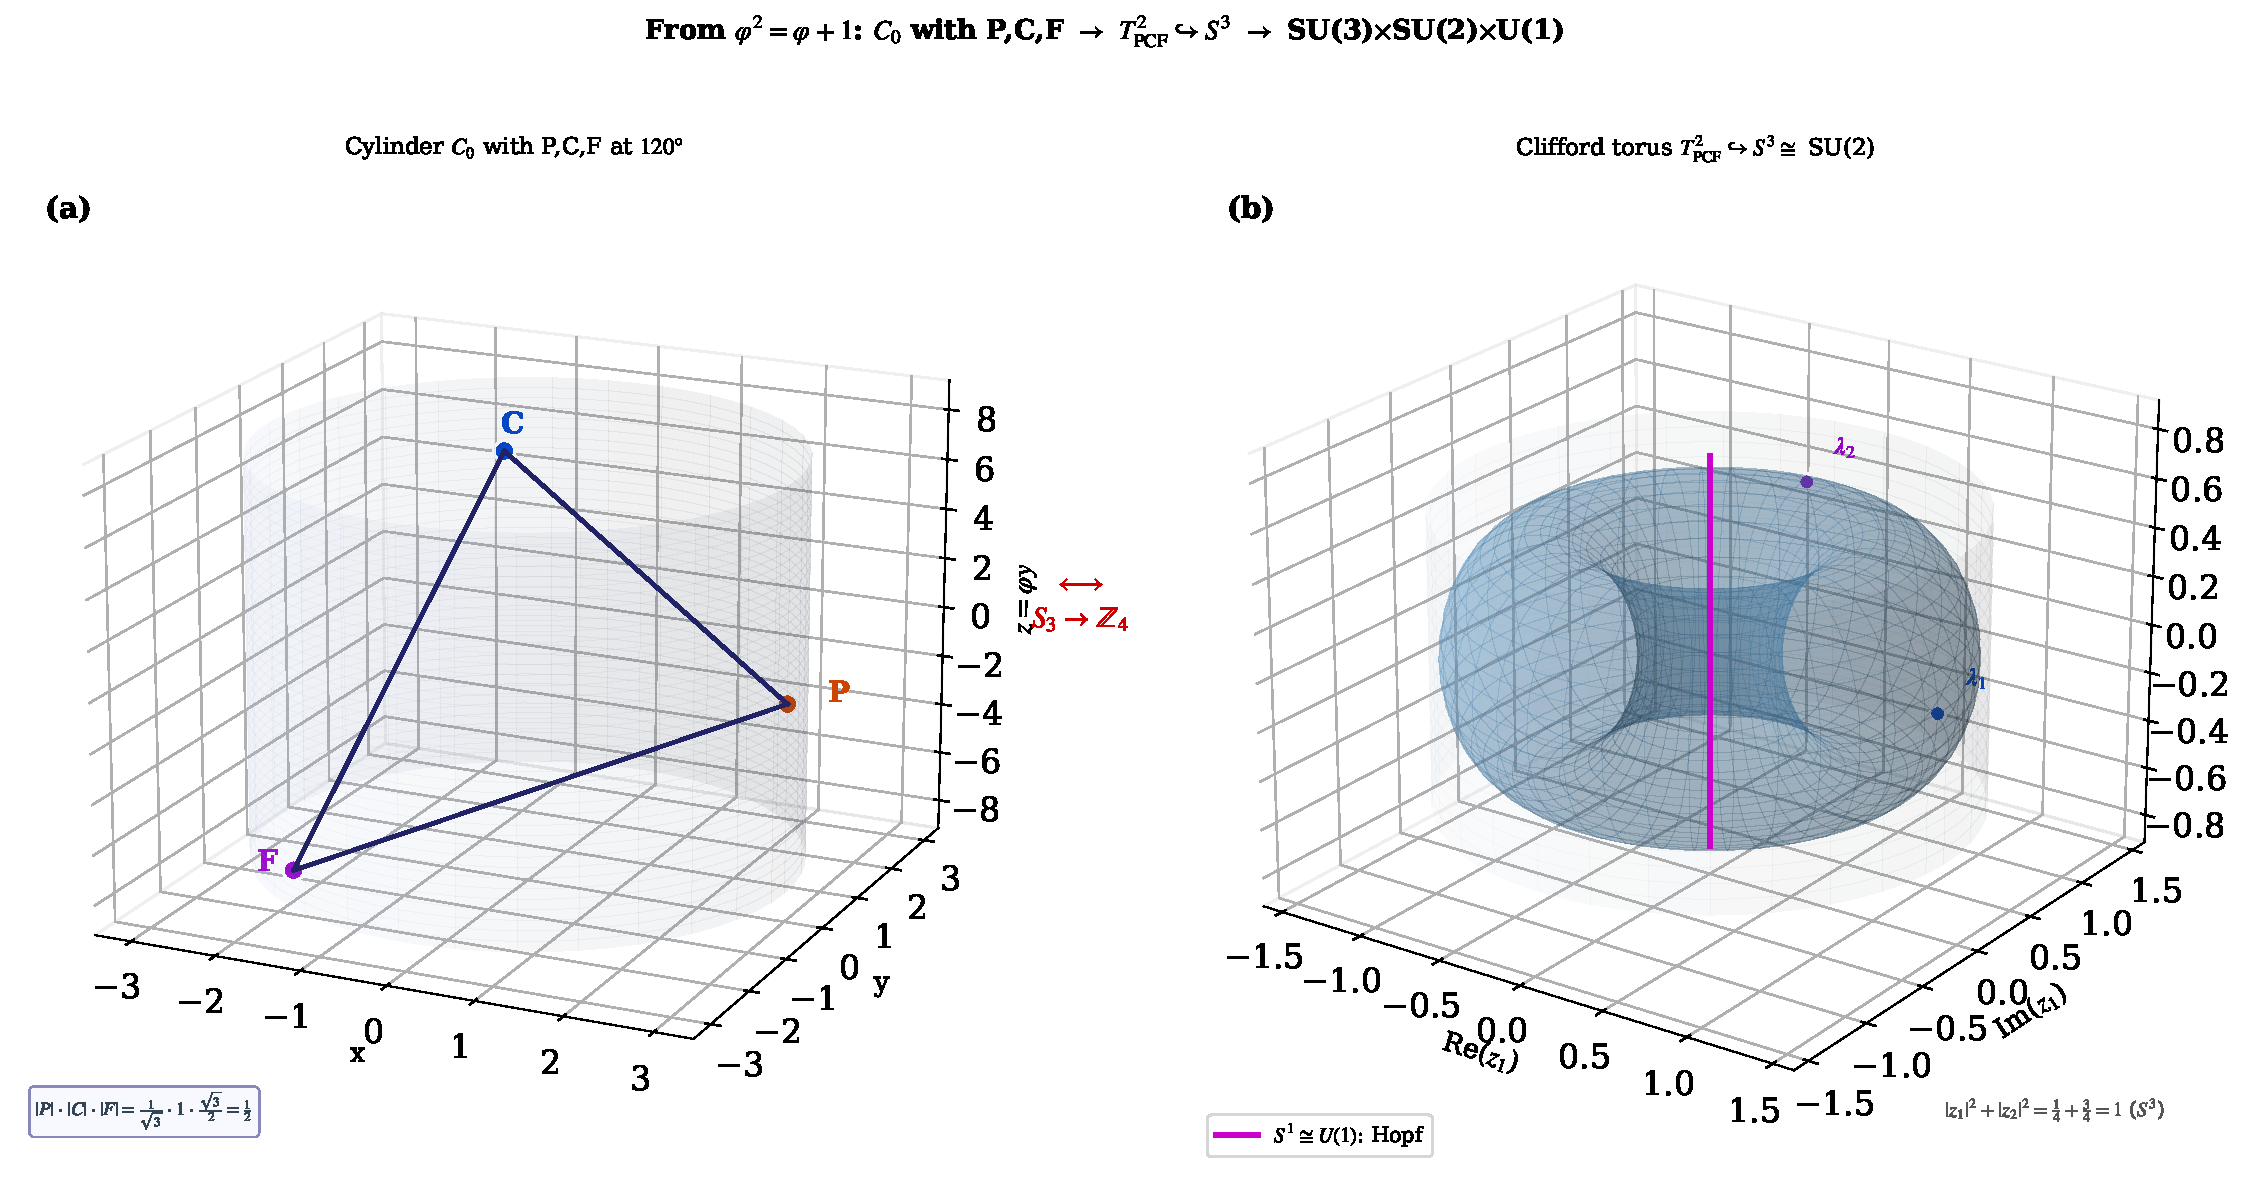
\includegraphics[height=0.82\textheight,keepaspectratio]{fig6_cylinder_torus.pdf}
\caption{From $\golden^{2}=\golden+1$: (a) the cylinder $C_0$ with $\mathrm{P,C,F}$ at $120^\circ$
($\|P\|\,\|C\|\,\|F\|=\tfrac12$) closes to (b) the torus $T^2_{\PCF}=\C/\Lambda$, $\tau=i$
($|z_1|^2+|z_2|^2=\tfrac14{+}\tfrac34=1$, the $S^3$ constraint), whose
Clifford embedding $T^2\hookrightarrow S^3$ and Hopf fibre give the gauge factors
$\mathrm{SU}(3)\times\mathrm{SU}(2)\times\mathrm{U}(1)$ of App.~\ref{app:gauge}.}
\label{fig:torus-gauge}
\end{figure}
\paragraph{Geometry and particle are the same object.}
The order of these facts is fixed by the diagram. The
projection $\Pi\colon\E^3\to\C$ is the \emph{root} of the whole downstream chain, and it is
at once the geometry of spacetime---the sheet and torus projected---and the particle. This
reflects the \emph{self-similarity} of the object: the same modulus $\tfrac12$ at every scale
level, seeded by $\golden^2=\golden+1$ extending $i^2=-1$ from the plane to space. The
particle carries the same geometry in its information and, as it accumulates entropy, keeps
it and moves within the spacetime geometry it itself is. There is no stage with geometry and
a later one with the particle: they are the same object at two scale readings. It is this
accumulation of information, carried by the self-similar geometry, that the next movement
reads as an observer (\S\ref{ssec:observer}): container and content, bulk and boundary,
geometry and particle are not separate---the same non-separation the M\"obius band already
fixed.

\emph{W1 --- the observer described by the theory (CLPW).} CLPW require (\S2.5) that the
observer be described by the theory, not introduced from outside. $\Pi$ is internal---no
external region from which to look---and self-similar, so the observer is the geometry itself
read at its centre. \emph{Proof:} \eqref{eq:obs-interface} with the bulk--boundary isometry
of \S\ref{sec:derivations}; Proposition~\ref{prop:obs-nofirewall};
\cite{CLPW22}. \ProofWitnessBlock{cw3\_observer\_items\_core}

\emph{W2 --- finite-dimensional Hilbert space (W01).} The finite horizon area requires finite
dimension; here the spectrum is the triangle of three eigenvalues and the mode count is
integer. \eqref{eq:obs-spinstar}. \ProofWitnessBlock{witten\_finite\_rank}

\subsection{The particle as observer}\label{ssec:observer}

What turns the particle into an observer is the accumulation of information, described
here by an internal Wick rotation, not imposed. When the centre is taken
as the time axis, its square changes sign, $(i\,t)^2=-t^2$ (\ProofWitness{wick\_squares\_flip\_sign, lorentzian\_signature\_sum}), and past and future become the two light cones, with the
apex---the present---as observer (\ProofWitness{C\_fixed\_PF\_rotate, causal\_trichotomy}). The
full metric is formalised in \S\ref{ssec:accum}; here the algebra of the rotation, which
is self-contained, suffices. The observer accumulates: its Fisher information grows to the
ceiling the Cram\'er--Rao bound permits,
\begin{equation}\label{eq:obs-fishertime}
  \tau_F=\frac{\tau_D}{\sqrt{2f}},\qquad \tau_F=\tau_D\iff f=\tfrac12 .
\end{equation}\begin{equation}\label{eq:obs-cramerrao}
  \mathrm{Var}(\theta)\ge F_\theta^{-1},\qquad
  \underbrace{\Fmax^{-1}=\tfrac14}_{\text{Kiely: Cram\'er--Rao}}
   \;=\;\underbrace{|\Om|^{2}=\mu_3^{2}=\tfrac14}_{\text{PCF area factor}} .
\end{equation}\begin{equation}\label{eq:obs-redundancy}
  R_\delta\sim N\ \ (\text{all fragments agree})\;\longleftrightarrow\;\text{objective record},
\end{equation}\begin{equation}\label{eq:obs-accum}
  F_\theta(t)\xrightarrow{\;N\to\infty\;}\Fmax\big(1-e^{-(t/\tau_F)^{2}}\big),\quad \Fmax=4,
  \qquad F_\Om=4\mu_3^{2}=1\ \text{bit},
\end{equation}
and sees exactly the half,
\begin{equation}\label{eq:obs-half}
  |P|\cdot|C|\cdot|F|=\tfrac12=|\Om| .
\end{equation}
The ``half'' is geometric: the eigenvalue dipole places $P$ at the south pole and $F$ at
the north, with $C$ the equatorial axis ($|C|=1$), and $|P|\,|F|=\tfrac14$ while $|C|=1$
gives the product $\tfrac12$; the $\sqrt3$ of $|F|$ cancels that of $|P|$---a cancellation
proper to the equilateral triangle, arity three (Proposition~\ref{prop:pcf-norms},
Proposition~\ref{prop:spectral}: $\sigma+\mu=2$, $\sigma\mu=\tfrac34$ with unique solution
$\mu=\tfrac12$, $\sigma=\tfrac32$.

\emph{W5 --- the initial--final pairing observable from within (W01).} Witten computes the
pairing $\langle f|i\rangle$ as calculable but not observable from outside (W01). It
becomes the internal pairing $\langle F|P\rangle=\bar F P/C$, with
$|\langle F|P\rangle|=\tfrac12$, observable because $\Pi$ is inside and no external region
remains. \emph{Proof:}

\emph{W3 --- the unitarity conjecture (W01).} Witten conjectures that the Hermitian
pairing is positive definite (W01). The spectrum is positive and $|\Om|=\tfrac12>\tfrac14$, so the object does not collapse.
\emph{Proof:}
(4.7).

The coincidence with Kiely's quantum Darwinism is forced, not numerical. The objectivity
threshold is $f_{\rm crit}=\tfrac12$; the redundancy grows as the mode number; the
certainty condition is $\varepsilon_0 M=\pi$:
\begin{equation}\label{eq:obs-threshold}
  \underbrace{f_{\mathrm{crit}}=\tfrac12}_{\text{Kiely: objectivity}}
   \;=\;\underbrace{|\Om|=\mu_3=\tfrac12}_{\text{PCF}},
\end{equation}\begin{equation}\label{eq:obs-certainty}
  \epsz\cdot\Mpcf=\pi\qquad(\text{cell capacity }=\pi\text{ bits}),
\end{equation}
\begin{proposition}[No separable parts before observation]\label{prop:no-parts}
For a pure two-party state let $p_1\ge p_2\ge\dots\ge0$ be the eigenvalues of the reduced state,
$\sum_i p_i=1$ (these are the squared Schmidt coefficients, $p_i=\lambda_i^2$; the criterion below
holds in this convention and not for the $\lambda_i$ themselves). The entanglement modulus is the
top eigenvalue, $|\Om|=p_1$, and it satisfies $|\Om|=|\Om|^{2}$ exactly when $p_1=1$---that is,
when every other $p_i$ vanishes, the reduced state is pure, the Schmidt rank is one and the state is
a product---and $|\Om|>|\Om|^{2}$ otherwise. The No-Diagonal fixes
$|\widehat\Om|=\tfrac12$ in the balanced (maximally entangled) case
(Proposition~\ref{prop:spectral}), so
\[
  |\Om|=\tfrac12\;>\;\tfrac14=|\Om|^{2},\qquad H(\tfrac12)=1\ \text{bit},
\]
the strict inequality being the signature of non-factorizability; for a product state it collapses to
$|\Om|=|\Om|^{2}=1$, $H=0$  (the Schmidt decomposition~\cite{Schmidt1907}) . Hence before observation there are no separable subsystems carrying \ProofWitness{no\_separable\_parts, separable\_iff\_top\_eigenvalue\_one}
values: what is real is the non-local whole, recovered as $|\widehat\Om|=\tfrac12$. PCF therefore
predetermines no parts, so it is neither a local-realist (Bell) nor a parts-realist (Leggett)
hidden-variable model, and the no-go theorems of~\cite{Bell64} and~\cite{Leggett03} do not bind it. 
\end{proposition}

The No-Diagonal theorem (\S\ref{ssec:arity}) establishes that every self-referential
structure without collapse must produce $\mu^2=\tfrac14$ and the tripartite
decomposition, with no other solution---which forces each identification. In the diagram,
here the first apex converges: three independent routes---the bridge (\S\ref{ssec:hinge}),
the triangle norm and the Fisher metric---give the same $\tfrac12$. When three independent
chains reach the same number, the diagram commutes at that point.

\subsection{The tower of information, and the emergence of curved spacetime}\label{ssec:accum}

\paragraph{The tower (types I and II interwoven).}
The accumulating observer does not select one reality among many: it builds it. There is
no landscape of vacua to choose from, no statistical ensemble to average. This
homogeneity---the same structure at every point---is what the field equations require: it
is the tensor covariance of \S\ref{ssec:hinge} now read as a constructive principle, and
its full development comes below. The entropy of one bit per cell, $H(\tfrac12)=1$
(\ProofWitness{binary\_entropy\_half}), is the maximally mixed state---$\rho_{\max}=1$ in CLPW's
language---describing the de~Sitter vacuum, and from its overflow the geometry is born.

When the $\pi$-bit cell fills, the throat opens:
\begin{equation}\label{eq:obs-throat}
  S(\sigma)=\pi\golden^{\sigma},
\end{equation}
with $N_{\rm modes}(\sigma)=\lfloor\pi\golden^\sigma\rfloor$. As it overflows, the throat
count is set:
\begin{equation}\label{eq:obs-swampland}
  \frac{|\partial_\sigma V|}{V}=\ln\golden=c_{\mathrm{PCF}} .
\end{equation}
The UV fixed point forces the invariants:
\begin{assumption}[The gauge--tower bridge]\label{asm:bridge}
\begin{equation}\label{eq:obs-fixedpoint}
  \beta_g(g^{*},\lambda^{*})=0\;\Longleftrightarrow\;\epsz\Mpcf=\pi .
\end{equation}
The right-hand side is derived and triply proved---in \S\ref*{ssec:construction} as
\eqref{eq:certainty}, here as \ProofWitness{eps0\_Mpcf\_pi}, and checked numerically \NumericalWitness{eq:certainty}; the equivalence itself is
this section's one input, the bridge between the gauge running and the tower's algebra. \Conj
\end{assumption}
The quantisation is in powers of $\golden$, and the identity that closes it is
$\golden^{-\lambda}=\tfrac12\Leftrightarrow\golden^\lambda=2$: the binary base comes out of
the golden geometry. Here the string reappears, not as a new object but as the same
particle in its information register: the dimension of the state space at each level is
$\dim\mathcal{H}(\sigma)=\lfloor S(\sigma)\rfloor$.

\emph{W4 --- the entropy conjecture (W01).} Witten conjectures that the Hilbert space is
finite-dimensional with $S=\ln N$ (W01). The Hilbert dimension per level is the integer
part of the horizon entropy, $\dim\mathcal{H}(\sigma)=\lfloor S(\sigma)\rfloor$, with
$N_{\rm modes}=\lfloor\pi\golden^\sigma\rfloor$---the constructive form of Witten's
$S=\ln N$. \emph{Proof:}
\ProofWitnessBlock{witten\_entropy\_realized, witten\_finite\_rank, witten\_two\_conjectures} (by \texttt{rfl}---the most direct realisation).
The entropy
branch is asserted strongly (tight); the unitarity branch is ``realised''.

The flow carrying one level to another, $\sigma\mapsto\sigma+t$, fixes $\tau=i$ and
preserves $\tfrac12$: it is the tracial flow, the type~II signature, and it is the thermal
flow of the static patch at the Gibbons--Hawking temperature.
\ProofWitnessBlock{tower\_scale\_group, tower\_flow\_fixes\_tau, omega\_flow\_group, omega\_flow\_invariant}

\emph{W11 --- the type~II algebra by crossed product (CLPW, completed).} CLPW build the
type~II$_1$ algebra from the type~III by the crossed product with the modular flow
(\S1.2--1.3). The scale flow preserves $\tfrac12$ as a trace, which is the type~II
signature; the section proves the flow and takes from CLPW the name of the crossed-product
classification. \emph{Proof:}
\ProofWitnessBlock{omega\_flow\_invariant, tower\_scale\_group}.

\emph{W12 --- the maximally mixed vacuum state (CLPW \S2.4, developed).} CLPW identify the
de~Sitter vacuum with the maximally mixed state, $\rho_{\max}=1$. One bit per cell,
$H(\tfrac12)=1$, gives that $\rho=1$ of maximal entropy. \emph{Proof:}
\ProofWitnessBlock{binary\_entropy\_half}.

The heart of the movement is that bulk and boundary are the same thing at once. The bulk
is the three-dimensional projection; the boundary, the two-dimensional plane; and they are
the same $\Pi$ of the first movement. The two accumulations---of time (Fisher) and of
scale (tower)---are one:
\begin{equation}\label{eq:obs-weld}
  \tau_F(\sigma)=\tau(\sigma)=\Mpcf\,\golden^{-\sigma},\qquad
  S(\sigma)\,\tau_F(\sigma)=\pi\Mpcf\ \ (\text{constant in }\sigma).
\end{equation}
The two lengths the tower carries are conjugate: the throat coordinate $z(\sigma)=\golden^{\sigma}$
grows with the level and the weld time $\tau(\sigma)=\Mpcf\golden^{-\sigma}$ shrinks with it, and
their product is constant,
\begin{equation}\label{eq:conjugate-pair}
  z(\sigma)\,\tau(\sigma)=\Mpcf\qquad\text{for every }\sigma .
\end{equation}
This is the relation $R\cdot(\alpha'/R)=\alpha'$ with $\alpha'=\Mpcf$: the compactification radius is
the throat coordinate, the lattice spacing is its T-dual, and $\alpha'$ is \emph{fixed by the product}
rather than chosen. Short and long distance are therefore the same family exchanged by duality, not two
regimes with a limit between them---the structural reason there is no ultraviolet regulator to remove
(Remark~\ref{rmk:residual}). \ProofWitnessBlock{lattice\_radius\_conjugate}

\begin{equation}\label{eq:obs-identity}
  \underbrace{F_\Om\cdot\Nmodes}_{\text{bits (Shannon)}}
   =\underbrace{S(\sigma)=\pi\golden^{\sigma}}_{\text{tower}}
   =\underbrace{\Nmodes=\lfloor S(\sigma)\rfloor}_{\text{matter}}
   =\underbrace{\SBH=\frac{A}{4\GN}}_{\text{horizon}}
   =\underbrace{S_{\text{Jacobson}}}_{\delta Q=T\delta S},
\end{equation}
This identification---the \emph{weld}---is where four routes converge, and it is the only
point where the three types coincide in one object: type~I by the discrete tower, type~II
by the observer's time, type~III because it lives on the spacetime. It is the maximal apex
of the diagram. Local and global are not separate: $\tfrac12$ at each level (local) and
invariant under the flow (global), the same invariant read two ways. Its last two branches
close below.

\paragraph{Curved spacetime (type III again).}
The accumulated entropy now sources gravity. Each bit costs---the Landauer cost, which is the
regulator $R_K=\log\golden$ of $\Q(\sqrt5)$ (Definition~\ref{def:regulator}) measured in
$\lambda_{\log}$, Theorem~\ref{thm:entropy-bridge},
$\lambda\cdot R=\log 2$---and when that cost is imposed as an equation of state
$\delta Q=T\,\delta S$ across every local Rindler horizon, the result is, by Jacobson's
argument, the Einstein equation:
\begin{equation}\label{eq:obs-landauer}
  \text{energy per bit}=\frac{1}{\Mpcf},\qquad
  \SBH/k_B=\lng\cdot R_K=\log2\ \ (\text{one bit; Theorem~\ref{thm:entropy-bridge}}),
\end{equation}\begin{equation}\label{eq:obs-jacobson}
  \delta Q=T\,\delta S\ \Longrightarrow\ \text{the Einstein equation},
\end{equation}\begin{equation}\label{eq:obs-einstein}
  R_{AB}=-4\,g_{AB},\quad R=-20,\qquad G_{AB}+\Lambda_5\,g_{AB}=\kappa\,T_{AB},\quad
  \kappa=8\pi\GN,
\end{equation}
with $G_N=\mu_3=\tfrac12$. Here the homogeneity of \S\ref{ssec:hinge} is redeemed:
Jacobson's argument requires a local horizon with the same law at every point---exactly
what tensor covariance guarantees; without it the step does not exist. The matter is the
mode number:
\begin{equation}\label{eq:obs-matter}
  T^{\mathrm{YM}}_{AB}=F_{AC}F_B{}^{C}-\tfrac14\,g_{AB}F_{CD}F^{CD},\qquad
  \text{matter}=\Nmodes=\lfloor S(\sigma)\rfloor .
\end{equation}
and here the two open branches of the identity close: the horizon entropy and Jacobson's
were, all along, the same number as the bits and the modes. Each mode is one bit exactly at the
modulus: the per-eigenvalue ceiling $F_\Om=4\mu_3^{2}$ is unity iff $\mu_3=\tfrac12$, and the
binary entropy there is $H(\tfrac12)=1$ bit.
\ProofWitnessBlock{fisher\_unit\_iff, H\_half\_one\_bit}%

That matter does not merely sit on the background: it curves it. The back-reaction is fixed by the
same modulus, with no free parameter, and it is what makes the shared root of \emph{metric} and
\emph{tension} (\S\ref{ssec:hinge}) a computation rather than an etymology.

\begin{definition}[Shell tension]\label{def:shell-tension}
A thin matter shell at the discrete level $w_\sigma=\sigma\log\golden$ of the throat
\eqref{eq:throat} has \emph{tension} $\lambda_\sigma$: its energy density per unit volume of the
constant-$w$ leaf. Its value is pinned by Proposition~\ref{prop:shell-tension}.
\ProofWitnessBlock{prop:shell-tension}%
\end{definition}

\begin{proposition}[The energy per bit is constant along the tower]\label{prop:ebit}
For every level,
\begin{equation}\label{eq:ebit}
  \frac{\varepsilon(\sigma)}{S(\sigma)}=\frac{\epsz}{\pi}=\frac{1}{\Mpcf},
\end{equation}
equivalently $S(\sigma)=\Mpcf\,\varepsilon(\sigma)$: the first law with temperature $T=1/\Mpcf$.
\ProofWitnessBlock{energy\_per\_bit\_constant}
\end{proposition}
\begin{proof}
The per-level energy is $\varepsilon(\sigma)=\epsz\golden^{\sigma}$ \eqref{eq:obs-accum} and the
saturation entropy is $S(\sigma)=\pi\golden^{\sigma}$ \eqref{eq:tower-modes}; the quotient cancels
$\golden^{\sigma}$ and leaves $\epsz/\pi$, which is $1/\Mpcf$ by the certainty relation
\eqref{eq:certainty}. The cancellation is what the common base buys: an energy growing at any other
rate would leave a $\sigma$-dependent residue.
\end{proof}

\begin{proposition}[The shell tension carries no free parameter]\label{prop:shell-tension}
The tension of Definition~\ref{def:shell-tension} is fixed by the level's mode count,
\begin{equation}\label{eq:shell-tension}
  \lambda_\sigma=\frac{\Nmodes(\sigma)}{\Mpcf}.
\end{equation}
\ProofWitnessBlock{shell\_tension\_determined}
\end{proposition}
\begin{proof}
Each tower mode is one bit: $\Nmodes(\sigma)=\lfloor S(\sigma)\rfloor$ \eqref{eq:obs-matter} is one
mode per bit of horizon entropy, and the Kiely ceiling $F_\Om=4\muthree^{2}=1$
\eqref{eq:obs-identity} makes each mode exactly one bit, neither more nor less. The shell's tension
is then the energy per bit times the number of bits,
$\lambda_\sigma=\varepsilon(\sigma)\Nmodes(\sigma)/S(\sigma)$, which is
$\Nmodes(\sigma)/\Mpcf$ by Proposition~\ref{prop:ebit}.
\end{proof}

\begin{proposition}[Israel junction: the back-reaction of each level]\label{prop:israel}
A constant-$w$ leaf of \eqref{eq:throat} has extrinsic curvature $K_{\mu\nu}=A'(w)g_{\mu\nu}$, so a
shell of tension $\lambda_\sigma$ imposes the jump
\begin{equation}\label{eq:israel}
  [A'(w_\sigma)]=-\frac{8\pi G_5}{3}\,\lambda_\sigma=-\frac{4\pi}{3}\,\lambda_\sigma,
  \qquad G_5=\muthree,
\end{equation}
and with \eqref{eq:shell-tension} the jump is determined level by level,
$[A'(w_\sigma)]=-\tfrac{4\pi}{3}\Nmodes(\sigma)/\Mpcf$. Between shells the metric is exact
$\mathrm{AdS}_5$: a steeper warp is a deeper curvature.
for the arithmetic; the junction condition itself~\cite{Israel66}. \ProofWitnessBlock{israel\_prefactor, israel\_jump\_determined}

\end{proposition}
\begin{proof}
The five-dimensional junction condition for a thin shell is
$[K_{\mu\nu}]=-8\pi G_5\bigl(S_{\mu\nu}-\tfrac13h_{\mu\nu}S\bigr)$; for pure tension
$S_{\mu\nu}=-\lambda h_{\mu\nu}$ this reduces to $[A']=-\tfrac{8\pi G_5}{3}\lambda$. With
$G_5=\muthree$ \eqref{eq:brown-henneaux} the prefactor collapses to $4\pi/3$---and only there: any
other Newton constant leaves $8\pi G_5/3\neq4\pi/3$.
\end{proof}

\begin{remark}[The cumulative back-reaction]\label{rmk:backreaction}
Each level kinks the warp---and deepens the local $|\Lambda|$---by an amount set by its mode count,
so the cumulative back-reaction up to level $k$ is $\sum_{\sigma\le k}\Nmodes(\sigma)$, giving
$3,8,16,29,50,84,140$ for $k=0,\dots,6$. The gravitational side and the string side are here the
same computation: \eqref{eq:israel} ties the extrinsic curvature to the shell tension, and
\eqref{eq:shell-tension} ties that tension to the mode count, so what curves the geometry is the
number of bits the level carries.
\ProofWitnessBlock{backreaction\_cumulative}
\NumericalWitnessBlock{eq:shell-tension}
\end{remark}

\noindent The cosmological constant is determined, not chosen:

\emph{W8 --- a theory that determines $\Lambda$ (W01).} The abstract of W01 states that
general relativity must be derived from a theory that \emph{determines} the value of
$\Lambda$. Here $\Lambda$ comes from the curvature, with zero free parameters:
$\Lambda_5=-d(d-1)/2\ell^2=-6$, with $\ell=1$ from \eqref{eq:bridge-S} (\S\ref{sec:derivations})
and $d=4$ from the arity (\S\ref{sec:methods}), and the G--$\Lambda$ duality
$\golden^{-6}\cdot\golden^{6}=1$ (\ProofWitness{G\_Lambda\_duality, R\_scalar\_pcf, BF\_value}).
Between the gravity scale and the $\Lambda$ scale there is an exact interval:

It remains to show the spacetime is de~Sitter. The metric obtained is Euclidean
anti-de~Sitter; the same internal Wick rotation that made the centre the time axis carries
it to de~Sitter, with $\varepsilon(\sigma)=\varepsilon_0\golden^\sigma$ and $\lambda$ the length
that converts the tower's logarithmic step into proper length along the scale axis, so that
$X_4=\lambda\ln s$ is the fifth, flat coordinate of \S\ref{app:embedding}:
\begin{equation}\label{eq:ets-metric}
  ds^{2}=\underbrace{(dx^{2}+dy^{2}+dz^{2})}_{\E^{3}}
        -\underbrace{c^{2}\,dt^{2}}_{\text{Wick }(C)}
        +\underbrace{\lambda^{2}\,d(\ln s)^{2}}_{\golden^{\sigma}\text{-tower}},
  \qquad s=\golden^{\sigma},
\end{equation}
It is the bridge to de~Sitter that Maldacena anticipated, built here by internal analytic
continuation rather than an imposed duality (\ProofWitness{ets\_is\_ds\_zero\_h}). Past and future
are the poles of a dipole, with $C$ at the equator---the two conjugate sheets of
de~Sitter.

\emph{W10 --- the antipodal map / meta-observables (W01).} The antipodal singularity
Witten notes corresponds to $F$ being antipodal to $P$ in the dipole, which resolves
Strominger's obstruction geometrically. \emph{Proof:} the dipole of \eqref{eq:ets-metric};
\cite{Witten01dS} (\S\ref{app:embedding}).

The geometric closure is the connection the framework contributes. The 5D ambient is
flat---its curvature, computed, vanishes, $R^{(5)}=0$ (\ProofWitness{ets\_constant\_block\_christoffels\_vanish})---and the
fifth coordinate, the scale axis, is the extra direction an embedding needs. De~Sitter is
the hyperboloid $-X_0^2+\cdots+X_4^2=1/H^2$ embedded in that flat ambient, with intrinsic
curvature ${}={}$ wedge of the extrinsic by Gauss: $R_{\mu\nu}=3H^2 g_{\mu\nu}$
(\ProofWitness{ds\_ricci\_from\_gauss, ds\_einstein\_lambda}). The planar patch covers exactly half
the hyperboloid---$X_0+X_4=\ell\,e^{t/\ell}>0$ never changes sign
(\ProofWitness{ds\_covers\_half\_hyperboloid})---and that half \emph{realises} the observer's half
$|\Om|=\tfrac12$ by the shared value (\ProofWitness{observer\_half\_from\_norms}). The assertoric
level splits: strong on the covering, ``realises'' on the identification.

\emph{W9 --- the thermal nature of the static patch (Gibbons--Hawking).} This is the
classical Gibbons--Hawking result, prior to W01 and CLPW: the de~Sitter horizon radiates
and the static patch is a thermal state at $T=H/2\pi$. The observer's modular flow is the
tracial flow of the tower, and the static patch is thermal at that temperature.
 (\S\ref{app:embedding}) \cite{GibbonsHawking77}. \ProofWitnessBlock{dS\_temperature, ds\_beta\_reciprocal}

\medskip
The formal statements underlying the accumulation and gravity movements follow; their
proofs are those of the corresponding \ProofWitness{...} tags.
\begin{remark}[The role of $\golden$ in the observer]
$\mu_3=\tfrac12=\golden^{-\lng}$; the three invariants ($f_{\mathrm{crit}}=\tfrac12$,
$\Fmax^{-1}=\tfrac14$, $n=3$) are $\golden$-facts of \S\ref{sec:methods}--\S\ref{sec:derivations},
not fitted values.
\end{remark}\begin{remark}[The role of $\golden$ in the objectivity threshold]
$|\Om|=\tfrac12=\mu_3=\golden^{-\lng}$: the half of de Sitter, Kiely's threshold and the modulus
are one $\golden$-fact; the throat that observation builds is the tower $\golden^{\sigma}$.
\end{remark}\begin{remark}[The role of $\golden$ in the accumulation]
$\epsz=\ln\golden/(6\sqrt3)$ and $\Mpcf=6\sqrt3\,\pi/\ln\golden$ give $\epsz\Mpcf=\pi$: the clock
of the accumulation, the ultraviolet fixed point and the certainty principle are one
$\golden$-fact; the accumulation tower is $\golden^{\sigma}$.
\end{remark}\begin{remark}[Past and future are fixed dynamically]
The reading of $C$-$P$-$F$ as present\,/\,past\,/\,future is not a free labelling but a consequence
of the causal structure. The Wick rotation makes the centre $C$ the time axis and gives the metric
of \eqref{eq:ets-metric} its Lorentzian signature $(+,+,+,-)$, so it carries a light cone: $C$ is
its apex---the observer's present---and $P,F$ are the past- and future-directed cones, rotating in
opposite senses about the fixed, real $C$, with $\Theta$ exchanging them. The direction of the
$\golden$-driven accumulation along the throat---from the origin toward the ceiling
(Proposition~\ref{prop:obs-accum})---orients the cone, singling out one direction as the future.
The past/future assignment therefore follows from the causal cone and the direction of
accumulation, not from convention.
\end{remark}\begin{proposition}[Accumulation and ceiling]\label{prop:obs-accum}
The metrological quantum Fisher information accumulates as
$F_\theta(t)\to\Fmax\bigl(1-e^{-(t/\tauF)^{2}}\bigr)$ with $\Fmax=4$~\cite{Kiely26},
so the Cram\'er--Rao ceiling $\Fmax^{-1}=\tfrac14=\muthree^{2}$ equals the
holographic area factor. The Fisher information per eigenvalue is
$F_{\Om}=4\muthree^{2}=1$ bit; the three eigenvalues give $3F_{\Om}=3=c$, the
central charge of \S\ref{ssec:object}; and the objectivity threshold
$f_{\mathrm{crit}}=\muthree=\tfrac12$ is the maximum-entropy point $H(\tfrac12)=1$ bit
(Proposition~\ref{prop:entropy-max}).
\ProofWitnessBlock{binary\_entropy\_half, S\_tower\_recurrence}
\NumericalWitnessBlock{prop:entropy-max}
\end{proposition}

\begin{theorem}[Time--scale conjugacy]\label{thm:obs-weld}
At the operating point $f=\muthree=\tfrac12$ the metrological timescale equals the
tower period, $\tauF(\sigma)=\tau(\sigma)=\Mpcf\,\golden^{-\sigma}$. Hence
\[
S(\sigma)\,\tauF(\sigma)=(\pi\golden^{\sigma})\,(\Mpcf\,\golden^{-\sigma})=\pi\Mpcf
\]
is constant in $\sigma$: the certainty principle $\epsz\Mpcf=\pi$
(\eqref{eq:certainty}) promoted from a single cell to the generation/clock pair.
\ProofWitnessBlock{obs\_weld}
\end{theorem}\begin{proposition}[The bulk metric is an Einstein space]\label{prop:obs-einstein}
For the warped throat \eqref{eq:throat} with $A=-\log z$ (anti-de~Sitter,
$\ell=1$), explicit computation of the Levi-Civita curvature gives, uniformly in
all five components,
\[
R_{AB}=-4\,g_{AB},\qquad R=-20,\qquad G_{AB}=6\,g_{AB}\quad(A,B=0,\dots,4),
\]
so the metric solves $G_{AB}+\Lambda_5\,g_{AB}=0$ with $\Lambda_5=-6$, and the
Breitenlohner--Freedman bound $m^{2}_{\mathrm{BF}}=-d^{2}/4=-4$ holds, so the discrete tower is
stable. With a
source, $G_{AB}+\Lambda_5\,g_{AB}=\kappa\,T_{AB}$ and $\kappa=8\pi\GN$; the PCF
value $\GN=\muthree=\tfrac12$ gives $\kappa=4\pi$ (effective $G_4=\tfrac14$), and
$\nabla^{A}G_{AB}=0$ holds identically, so $T_{AB}$ is conserved.
\ProofWitnessBlock{G\_AB\_pcf, R\_AB\_einstein, R\_scalar\_pcf, einstein\_coeff, ricci\_coeff, ricci\_scalar, BF\_value}
\end{proposition}

\begin{theorem}[Jacobson's construction on the bulk metric]\label{thm:obs-jacobson}
Since \eqref{eq:throat} is an Einstein space, $R_{ab}k^{a}k^{b}=-4\,g_{ab}k^{a}k^{b}=0$
for every null $k$; in vacuum the Clausius relation
$\delta Q=\int T_{ab}\chi^{a}\,d\Sigma^{b}=0$ forces $\delta S=0$ (Jacobson's
entanglement equilibrium~\cite{Jacobson1995}), which coincides with the ceiling
$\Fmax^{-1}=\muthree^{2}$ of Prop.~\ref{prop:obs-accum}. The normalisation
$\eta=1/4\GN$ with $\GN=\muthree$ fixes the area factor $\muthree^{2}=\tfrac14$
and the coupling $2\pi/\eta=8\pi\GN$; with matter, $\delta Q=T\,\delta S$ on every
local Rindler horizon yields the Einstein equation~\cite{Jacobson1995,Jacobson2016}.
\ProofWitnessBlock{ds\_einstein\_lambda, R\_AB\_einstein, G\_AB\_pcf}
\end{theorem}

\begin{proposition}[Matter is the saturation entropy]\label{prop:obs-matter}
Each interior level carries $\Nmodes(\sigma)=\lfloor\pi\golden^{\sigma}\rfloor
=\lfloor S(\sigma)\rfloor$ scalar modes, each contributing one Shannon bit, so the
matter content of level $\sigma$ is the saturation entropy $S(\sigma)=\pi\golden^{\sigma}$. That
this is an \emph{equality} and not merely a count is the first law of the tower: the Kiely ceiling
$F_\Om=4\muthree^{2}=1$ makes each mode exactly one bit (Proposition~\ref{prop:obs-accum}), the
per-level energy is $\varepsilon(\sigma)=\epsz\golden^{\sigma}$ with $\epsz\Mpcf=\pi$, so the energy
per bit is constant across the tower (Proposition~\ref{prop:ebit}),
\begin{equation}
  \frac{\varepsilon(\sigma)}{S(\sigma)}=\frac{\epsz}{\pi}=\frac1{\Mpcf},
\end{equation}
which is $S(\sigma)=\Mpcf\,\varepsilon(\sigma)$ at temperature $T=1/\Mpcf$
The colour octet has $\dim\mathfrak{su}(3)=n^{2}-1=8$ at the arity
$n=3$ fixed by the golden central chain $\golden^{2}+\golden^{-2}=3$; the full
$\mathrm{SU}(3)\times\mathrm{SU}(2)\times\mathrm{U}(1)$ follows from the torus $T^2_{\PCF}$
\eqref{eq:torus}, its gauge factors landing at the force levels by increasing dimension
$1<3<8$: $\mathrm{U}(1)$ is the Hopf fibre $S^1$ at $\sigma=3$ (EM), $\mathrm{SU}(2)$ the Clifford
$S^3$ at $\sigma=4$ (weak), and $\mathrm{SU}(3)$ the $A_2$ roots of the Eisenstein face
(Fig.~\ref{fig:isometry-algebra}) at $\sigma=5$ (strong), with $\dim\mathfrak{su}(3)=n^{2}-1=8$ at
the arity $n=3$ fixed by the golden central chain $\golden^{2}+\golden^{-2}=3$
\ProofWitnessBlock{gauge\_dim\_su3, phi\_central\_chain, central\_chain, KK\_numerator, clifford\_S3\_condition, hopf\_from\_clifford, a2\_minimal\_vectors\_exactly\_six}.

The electroweak data follow from the same modulus: the weak mixing angle at unification is
$\sin^{2}\theta_W|_{\rm GUT}=\tfrac38=N(0)/N(2)$ \ProofWitness{weinberg\_angle\_gut}
running to $0.231$ at
$M_Z$; the tower entropy ratio $S(3)/S(6)=\golden^{-3}$ \ProofWitness{entropy\_ratio\_S3\_S6} marks the
breaking $\Z_3\to\Z_4$ at the tower midpoint $\sigma=3$, and the $G$--$\Lambda$ duality reads $\golden^{-6}\golden^{+6}=1$
The generations are not placed radially by this $\sigma$-assignment:
the charged-lepton ratios are not integer powers of $\pi$ ($m_\mu/m_e=\pi^{4.66}$), and a
$\pi$-graded radial triple cannot satisfy the Koide relation. Two statements are at work here, of different objects: the Koide ratio $Q=\tfrac23$ is an algebraic identity of that placement form, holding for every $\delta$ and hence no evidence for any particular value; the prediction is the three masses themselves, reconstructed to $\sim10^{-4}$ from the single scale $\sqrt M$ with $\delta=2/n^{2}$ fixed by the arity, a value so sharply selected that a $0.1\%$ departure degrades the fit by two orders of magnitude. The $\sigma$-levels label sectors and
forces; the three generations are the \emph{angular} $\omega$-triple within a sector, placed in the
bridge with no free angular parameter,
$\sqrt{m_k}=\sqrt M\,(1+\sqrt2\cos(\delta+2\pi k/3))$ with $\delta=2/n^{2}=\tfrac29$ at arity $n=3$,
reconstructing the three charged-lepton masses to ${\sim}10^{-4}$ from the single scale $\sqrt M$.
That scale is not an independent input: the certainty condition $\varepsilon_0 M=\pi$ \eqref{eq:obs-threshold} is the same that fixes $\Mpcf$, so $M=\Mpcf$; Theorem~\ref{thm:colour-from-M} then derives the colour scale and running from it. What remains open is only the quark spectrum and its CKM mixing, not the scale or the colour running.   (bridge)% \ProofWitness{M\_eq\_Mpcf}
Their Yang--Mills stress-energy
$T^{\mathrm{YM}}_{AB}=F_{AC}F_{B}{}^{C}-\tfrac14\,g_{AB}F_{CD}F^{CD}$ is
conserved ($\nabla^{A}T^{\mathrm{YM}}_{AB}=0$) and traceless on the
$D=4$ worldsheet (conformal there).
\end{proposition}

\begin{theorem}[The Landau--Lifshitz energy of the field]\label{thm:LL-energy}
On the de~Sitter background \eqref{eq:ets-metric} with $\GN=\muthree=\tfrac12$, the Landau--Lifshitz complex $(-g)(T^{\mu\nu}+t_{\mathrm{LL}}^{\mu\nu})=\tfrac1{16\pi\GN}\partial_\alpha\partial_\beta H^{\mu\alpha\nu\beta}$ has vanishing energy density---its $00$ component is zero, the net energy of matter and field balancing, the classical face of the entanglement equilibrium $\delta S=0$ of Theorem~\ref{thm:obs-jacobson}---while its spatial components $-2H^{2}e^{4Ht}/\pi$ do not vanish, as de~Sitter is not static (the standard complex differs from the physical vacuum pressure by the $\Lambda$-term the pseudotensor requires for $\Lambda\neq0$). The gravitational energy is a definite boundary charge: the energy in the Hubble volume $\rho_\Lambda V_H=1/H=T_{\mathrm{GH}}\,S_{\mathrm{GH}}$ is the first law of de~Sitter, and the Komar/Landau--Lifshitz charge of the horizon $\kappa A/(8\pi\GN)$ gives the same $1/H$. The modulus $\muthree=\tfrac12$ is the ratio $T_{\mathrm{GH}}/T_{\mathrm{local}}$ of horizon and local temperatures. The gravitational field energy---absent from $\nabla^{A}T_{AB}=0$ (Proposition~\ref{prop:obs-matter})---is thus fixed, the energy conjugate to the tower entropy $S(\sigma)$ by the first law.
\ProofWitnessBlock{ds\_first\_law, energy\_is\_inv\_H, komar\_first\_law, mu3\_temp\_ratio, LL\_spatial\_ne\_zero}
\NumericalWitnessBlock{eq:obs-landauer}
\end{theorem}\begin{remark}[The G--$\Lambda$ interval: $\Lambda$ is determined, not selected]
\label{rmk:GLambda-interval}
The cosmological constant is not an input. The scale $\ell=1$ (from the
S-duality fixed point $\tau=i$, \eqref{eq:bridge-S}) and the dimension $d=4$
(from the arity $n=3$, \S\ref{ssec:arity}) are both derived, and they fix
\begin{equation}\label{eq:Lambda-from-curvature}
  \Lambda_5=-\frac{d(d-1)}{2\ell^{2}}=-6 ,
\end{equation}
with zero free parameters. The $6$ arrives by two independent routes---the curvature magnitude
$|\Lambda_5|=d(d-1)/2$ and the tower ceiling $\sigma_\Lambda=2n$ of \eqref{eq:interval-levels}---and
the routes agree only at the arity: $(n{+}1)n/2=2n$ forces $n=3$.
\ProofWitnessBlock{two\_routes\_to\_six}%
This realises precisely what
Witten~\cite{Witten01dS} identified as necessary: a theory
``that determines the value of the cosmological constant.''

\emph{The tower levels.} The activation levels of the three sectors are read
off the arity, not postulated:
\begin{equation}\label{eq:interval-levels}
  \sigma_G=n-1=2,\qquad \sigma_{\mathrm{EM}}=n=3,\qquad \sigma_\Lambda=2n=6 .
\end{equation}
Gravity activates at $\sigma_G=n-1$ (the spatial bulk $\E^{3}$ complete, one
dimension below the bulk); the electromagnetic sector sits at the midpoint
$\sigma_{\mathrm{EM}}=n$ (the Page point that halves the tower $[0,2n]$); and
$\Lambda$ activates at the ceiling $\sigma_\Lambda=2n$. The ceiling is
geometric: the torus $T^{2}_{\PCF}$ is a \emph{complex} space, so complex
dimension $n$ is real dimension $2n$---``complex dimension three'' is
$\R^{6}$, never $\R^{3}$. The tower runs over the full real space
$\sigma\in\{0,1,\dots,2n\}$, and its ceiling $\sigma_\Lambda=2n$ is that real
dimension.

\emph{The interval is the spacetime.} The gap between the gravity and
$\Lambda$ levels is exactly the dimension of spacetime,
\begin{equation}\label{eq:interval-gap}
  \sigma_\Lambda-\sigma_G=2n-(n-1)=n+1=4=\dim(M^{4}),
\end{equation}
and the interval carries the two holographic invariants of the microstate:
\begin{equation}\label{eq:interval-fractions}
  \frac{\sigma_{\mathrm{EM}}-\sigma_G}{\sigma_\Lambda-\sigma_G}
    =\frac{1}{n+1}=\frac14=|\Om|^{2}
  \qquad\text{and}\qquad
  \frac{\sigma_{\mathrm{EM}}-\sigma_G}{\sigma_\Lambda-\sigma_{\mathrm{EM}}}
    =\frac1n=\frac13=\|P\|^{2},
\end{equation}
the holographic area factor $\tfrac14=|\Om|^{2}$ and the past-component
weight $\tfrac13=\|P\|^{2}=F_\Om/c$.

\emph{Two independent routes to the same $6$.} The curvature magnitude
$|\Lambda_5|=d(d-1)/2=6$ (from $d=4$) and the tower ceiling
$\sigma_\Lambda=2n=6$ (from $n=3$, as the real dimension of the complex
torus) coincide by independent routes---5D curvature on one side, the
real dimension of the worldsheet torus on the other. Both are the entropy
saturation of the microstate read geometrically: $\sigma_\Lambda=2n=6$ is the
ceiling of the golden tower $S(\sigma)=\pi\golden^{\sigma}$ whose accumulated
bits are the horizon entropy of \eqref{eq:obs-identity} and, through
\eqref{eq:obs-einstein}, the field equations---the six-fold value is that
saturation, not a separate geometric fact. Together with $6=|S_{3}|=3!$ (the order of the symmetry
group, Lem.~\ref{lem:s3-orders}) and the exponent of the $G$--$\Lambda$ duality
$\golden^{-6}\golden^{+6}=1$, the value $\sigma_\Lambda=6$ is fixed from
four sides.

\emph{Scope.} This we propose as the structure Witten required: the de~Sitter
Hilbert-space dimension $N$ is integer, so $G\Lambda^{(n-2)/n}$ cannot vary
continuously and both $G$ and $\Lambda$ must be fixed by a more fundamental
theory~\cite{Witten01dS}; here $\GN=\tfrac12$ and $\Lambda\sim\golden^{-6}$, the
product fixed, $\golden^{-6}\golden^{+6}=1\iff G\Lambda\sim
M_{\mathrm{Pl}}^{-4}M_{\mathrm{Pl}}^{4}=1$ (PCF units). What is determined is this
dimensionless conjugacy. The translation to the observed
$\Lambda_{\mathrm{obs}}\sim10^{-122}M_{\mathrm{Pl}}^{4}$ is a matter of scale translation, not
derived here; and it is a \emph{single} open item rather than two. The level the observer occupies
is not an independent parameter: the tower fixes it from the de~Sitter entropy, and that entropy is
$1/\Lambda$, so
\begin{equation}\label{eq:sigma-obs}
  \sigma_{\mathrm{obs}}=\frac{\ln(S_{dS}/\pi)}{\ln\golden},\qquad
  S_{dS}=\frac{3\pi}{\GN\Lambda}\ \overset{\GN=1/2}{=}\ \frac{6\pi}{\Lambda}
  \quad\Longrightarrow\quad
  \sigma_{\mathrm{obs}}=\frac{\ln(6/\Lambda_{\mathrm{obs}})}{\ln\golden}.
\end{equation}
Deriving the scale translation therefore derives the level, and conversely; counting them as two
debts would be an accounting error. The scale $\sqrt M$ that sets the charged leptons (\S\ref{prop:obs-matter}) is therefore the tower reading of this de~Sitter entropy, and Theorem~\ref{thm:colour-from-M} then shows the colour sector hanging on the same scale: one scale surfaces as the string constant of \S\ref{sec:derivations} and as the entropy here, the dimensionless placement already fixed, the absolute value alone carrying the observer's $\Lambda$. What the tower does add is granularity: its step is exactly
$\golden$ ($\log_{10}\golden=0.209$ per level), so the absolute scale is constrained to a discrete
ladder rather than a continuum.
\NumericalWitnessBlock{eq:Lambda-from-curvature}
\ProofWitnessBlock{lambda\_magnitude\_eq\_level, sigma\_G\_val, sigma\_EM\_val, sigma\_Lambda\_val, threshold\_ordering, interval\_gap, interval\_gap\_general, em\_holographic\_fraction, em\_asymmetry, entropy\_at\_mu\_three, tower\_step\_ratio}
\end{remark}

\begin{proposition}[The level triple is unique over the integers]\label{prop:interval-uniqueness}
Consider integer triples $\sigma_G<\sigma_{\mathrm{EM}}<\sigma_\Lambda$ subject to the four
conditions already in place: the ceiling $\sigma_\Lambda=2n$, the gap
$\sigma_\Lambda-\sigma_G=n+1$ \eqref{eq:interval-gap}, and the two fractions of
\eqref{eq:interval-fractions} equal to the microstate invariants,
\begin{equation}\label{eq:interval-unique}
  \frac{\sigma_{\mathrm{EM}}-\sigma_G}{\sigma_\Lambda-\sigma_G}=|\Om|^{2}=\tfrac14,
  \qquad
  \frac{\sigma_{\mathrm{EM}}-\sigma_G}{\sigma_\Lambda-\sigma_{\mathrm{EM}}}=\|P\|^{2}=\tfrac13 .
\end{equation}
At the arity $n=3$ of \S\ref{ssec:arity} the four are satisfied by exactly one triple,
$(\sigma_G,\sigma_{\mathrm{EM}},\sigma_\Lambda)=(2,3,6)$, which is the assignment
\eqref{eq:interval-levels}. The selection is by the arity and not by fitting: the family
$(n-1,n,2n)$ satisfies the two fractions as $1/(n+1)$ and $1/n$ for \emph{every} $n$, and only
$n=3$ carries them onto $|\Om|^{2}=\tfrac14$ and $\|P\|^{2}=\tfrac13$ of
\eqref{eq:norms-derived}---at $n=2$ they are $\tfrac13,\tfrac12$ and at $n=4$ they are
$\tfrac15,\tfrac14$. Equivalently, $\sigma_\Lambda-\sigma_G=n+1$ equals $4=\dim(M^{4})$ only at
$n=3$. This is what Fig.~\ref{fig:alpha-uniqueness} displays --- panel (b) the constraint count,
panel (a) the spectral-angle surface of \S\ref{ssec:meta} evaluated on the resulting pair --- and it
is what lets
\S\ref{ssec:meta} read the spectral angle at the integer pair
$(\sigma_G,\sigma_{\mathrm{EM}})=(2,3)$ without circularity: the levels come from the arity, and
the angle is then evaluated on them. \ProofWitnessBlock{interval\_uniqueness, interval\_arity\_discriminates, interval\_gap\_only\_three}

\end{proposition}
\begin{proof}
Write $a=\sigma_{\mathrm{EM}}-\sigma_G>0$ and $b=\sigma_\Lambda-\sigma_{\mathrm{EM}}>0$, so
$\sigma_\Lambda-\sigma_G=a+b$. The second fraction of \eqref{eq:interval-unique} is $a/b=\tfrac13$,
i.e.\ $b=3a$; the first is then $a/(4a)=\tfrac14$ identically, so the two fractions are one
condition. The gap gives $a+b=4a=n+1$, whence $a=1$ at $n=3$ and $b=3$; the ceiling gives
$\sigma_\Lambda=6$, hence $\sigma_G=6-4=2$ and $\sigma_{\mathrm{EM}}=3$. Uniqueness is that each
step determined its unknown. For the discrimination, $(n-1,n,2n)$ gives $a=1$, $b=n$, $a+b=n+1$, so
the fractions are $1/(n+1)$ and $1/n$; these equal $\tfrac14$ and $\tfrac13$ iff $n=3$.
\end{proof}

\begin{figure}[!htbp]\centering
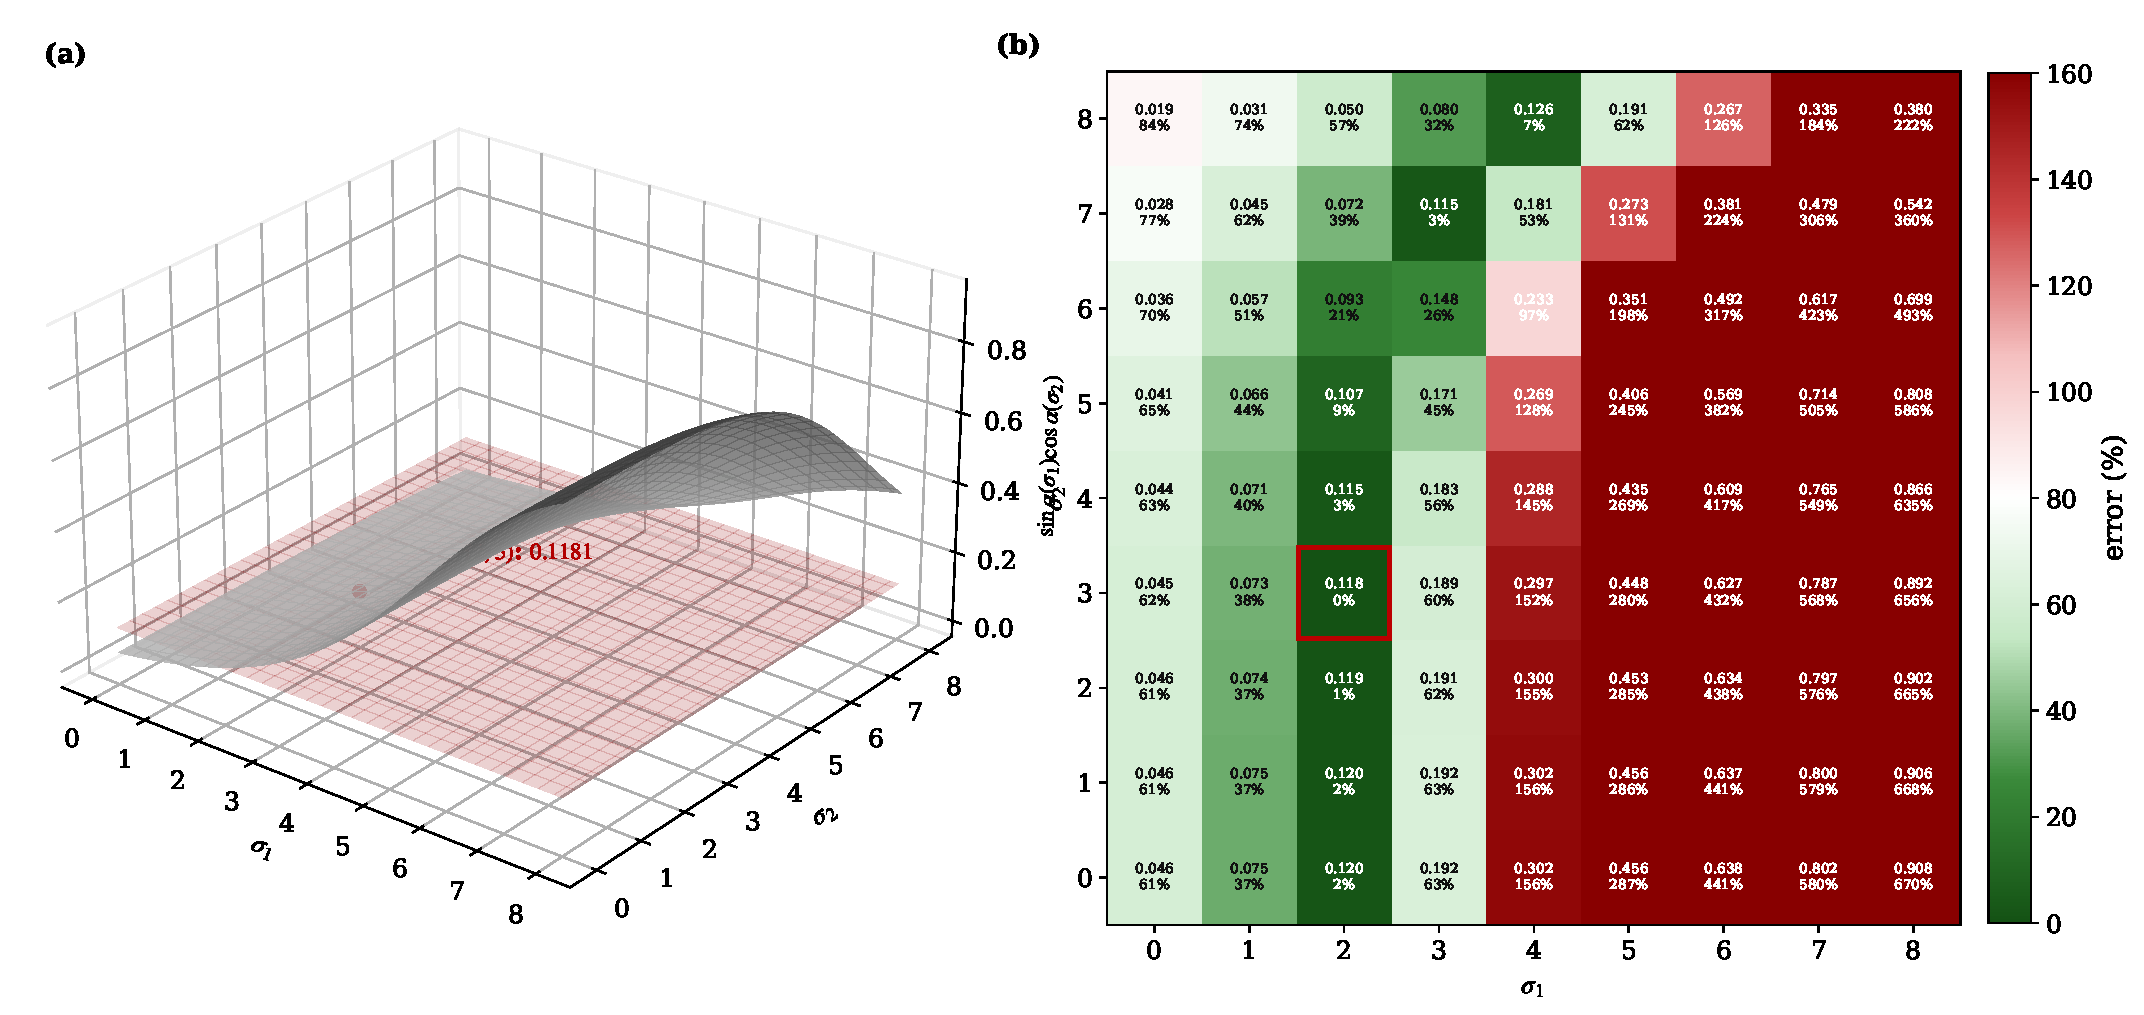
\includegraphics[height=0.82\textheight,keepaspectratio]{fig1_alphas_uniqueness.pdf}
\caption{(a) The spectral-angle surface $\sin\alpha(\sigma_1)\cos\alpha(\sigma_2)$ of
\eqref{eq:spectral-surface}; $\tan\alpha(\sigma{+}1)/\tan\alpha(\sigma)=\golden$
(\eqref{eq:spectral-angle}). The marked point $(2,3)$ gives
$\sin\alpha(2)\cos(3)=0.1181\approx\sin\alpha_{\rm GUT}$.
(b) Constraint count for each triple $(\sigma_G,\sigma_{\mathrm{EM}},\sigma_\Lambda)$:
$\sigma_\Lambda=2n$, $\sigma_\Lambda-\sigma_G=n{+}1$,
$(\sigma_{\mathrm{EM}}{-}\sigma_G)/(\sigma_\Lambda{-}\sigma_G)=|\Om|^2$,
$(\sigma_{\mathrm{EM}}{-}\sigma_G)/(\sigma_\Lambda{-}\sigma_{\mathrm{EM}})=\|P\|^2$.
Only $(2,3,6)$ satisfies all four (boxed). No fitted quantity enters.}
\label{fig:alpha-uniqueness}
\end{figure}

\subsection{Why this is a single demonstration}\label{ssec:spine4}

The path went through the three types: it opened in the non-local type~III field, made the
type~I particle emerge, turned it into the type~II observer, interwove I and II in the
tower, and closed in the type~III spacetime. These are not five demonstrations glued
together but one, because the same object of modulus $\tfrac12$ is the protagonist of all,
and each transition is a proved implication: entropy orients the flow and yields the
particle, the Wick rotation gives the cones and the observer, accumulation overflows and
builds the tower, entropy sources gravity.

The commutative diagram supports this unity with precise structure. The twenty-four
equations form a directed acyclic graph with two roots---the projection $\Pi$
(\eqref{eq:obs-interface}) and the observer's objective record
(\eqref{eq:obs-redundancy})---from which all else derives, with $36$ demonstrative edges.
A topological order exists---the equations can be stated so that none depends on a later
one---which guarantees the section reads without forward reference. Eight nodes are apices,
where two or more independent chains converge; the weld (\eqref{eq:obs-weld}), with four
routes, is the maximal one and the only triple point I${\cap}$II${\cap}$III. The circle
closes literally: \eqref{eq:obs-einstein} returns to \eqref{eq:obs-interface}---the
non-local gravity returns to the same $\Pi$ and $\tfrac12$ of the opening, III${\to}$III.
The spacetime at the end is non-local at every point, type~III, as the field at the start,
and its Newton constant is the same $\tfrac12$ of the object one began with. One enters by
any door and reaches the same object: that is what it means for the diagram to commute.
The section does not prove six things; it proves that an observer of modulus $\tfrac12$,
which cannot be separated into parts, is at once the particle, the string, the tower of
information and the curved de~Sitter universe that contains it, and that this universe has
the $\Lambda$ the theory was bound to determine, with the observer inside. The debt with
which the section opened is settled by the same object that raised it.

\medskip\noindent\textbf{The demonstrative line.} Each step uses only the previous ones.

\begin{figure}[htb]\centering
\resizebox{\textwidth}{!}{%
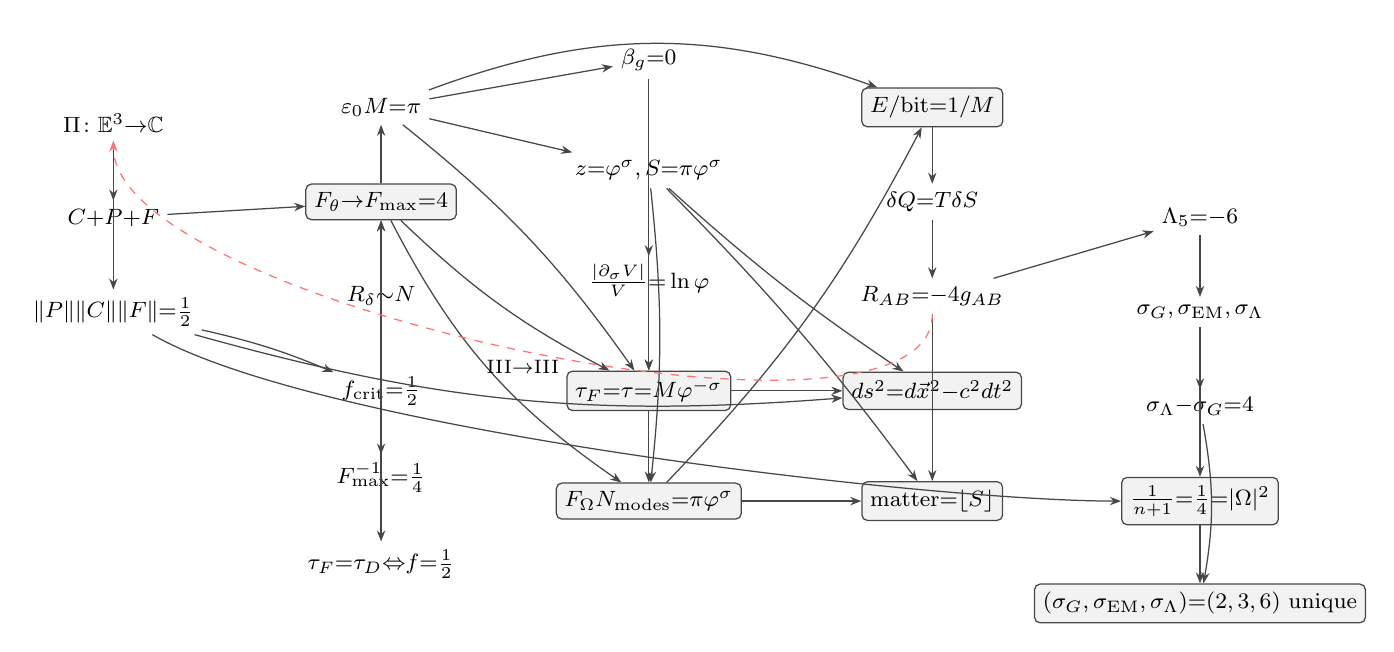
\begin{tikzpicture}[
  font=\footnotesize,
  >={Stealth[length=4pt]},
  nd/.style={inner sep=2pt, outer sep=1pt},
  ap/.style={draw, rounded corners=2pt, fill=black!5, inner sep=3pt},
  every path/.style={->, draw=black!72, line width=0.45pt}]

% ===== 4.2 field + particle (x=0) =====
\node[nd] (int) at (0,5.4)  {$\Pi\colon\E^3{\to}\C$};
\node[nd] (spin) at (0,4.2) {$C{+}P{+}F$};
\node[nd] (half) at (0,3.0) {$\|P\|\|C\|\|F\|{=}\tfrac12$};

% ===== 4.3 observer (x=3.4) =====
\node[nd] (thr)  at (3.4,2.0) {$f_{\rm crit}{=}\tfrac12$};
\node[nd] (cram) at (3.4,0.9) {$\Fmax^{-1}{=}\tfrac14$};
\node[nd] (fish) at (3.4,-0.2){$\tau_F{=}\tau_D{\Leftrightarrow}f{=}\tfrac12$};
\node[nd] (red)  at (3.4,3.2) {$R_\delta{\sim}N$};
\node[ap] (acc)  at (3.4,4.4) {$F_\theta{\to}\Fmax{=}4$};
\node[nd] (cert) at (3.4,5.6) {$\varepsilon_0 M{=}\pi$};

% ===== 4.4 tower (x=6.8) =====
\node[nd] (fix)    at (6.8,6.2) {$\beta_g{=}0$};
\node[nd] (throat) at (6.8,4.8) {$z{=}\golden^\sigma,S{=}\pi\golden^\sigma$};
\node[nd] (swp)    at (6.8,3.4) {$\tfrac{|\partial_\sigma V|}{V}{=}\ln\golden$};
\node[ap] (weld)   at (6.8,2.0) {$\tau_F{=}\tau{=}M\golden^{-\sigma}$};
\node[ap] (id)     at (6.8,0.6) {$F_\Om\Nmodes{=}\pi\golden^\sigma$};

% ===== 4.4 gravity (x=10.4) =====
\node[ap] (land) at (10.4,5.6) {$E/\text{bit}{=}1/M$};
\node[nd] (jac)  at (10.4,4.4) {$\delta Q{=}T\delta S$};
\node[nd] (ein)  at (10.4,3.2) {$R_{AB}{=}{-}4g_{AB}$};
\node[ap] (ets)  at (10.4,2.0) {$ds^2{=}d\vec x^2{-}c^2dt^2$};
\node[ap] (mat)  at (10.4,0.6) {$\text{matter}{=}\lfloor S\rfloor$};

% ===== 4.5 Lambda + interval (x=13.8) =====
\node[nd] (lam)  at (13.8,4.2) {$\Lambda_5{=}{-}6$};
\node[nd] (lev)  at (13.8,3.0) {$\sigma_G,\sigma_{\rm EM},\sigma_\Lambda$};
\node[nd] (gap)  at (13.8,1.8) {$\sigma_\Lambda{-}\sigma_G{=}4$};
\node[ap] (frac) at (13.8,0.6) {$\tfrac1{n+1}{=}\tfrac14{=}|\Om|^2$};
\node[ap] (uniq) at (13.8,-0.7) {$(\sigma_G,\sigma_{\rm EM},\sigma_\Lambda){=}(2,3,6)$ unique};

% ===== edges (columna a columna, como spine3) =====
\draw (int) -- (half);
\draw (int) -- (spin);
\draw (spin) -- (acc);
\draw (half) to[bend left=5] (thr);
\draw (thr) -- (cram);
\draw (thr) -- (fish);
\draw (cram) -- (acc);
\draw (red) -- (acc);
\draw (acc) -- (cert);
\draw (cert) -- (fix);
\draw (cert) -- (throat);
\draw (throat) -- (swp);
\draw (fix) -- (weld);
\draw (acc) to[bend right=8] (weld);
\draw (throat) -- (weld);
\draw (cert) to[bend left=8] (weld);
\draw (weld) -- (id);
\draw (throat) to[bend left=6] (id);
\draw (acc) to[bend right=14] (id);
\draw (id) to[bend right=8] (land);
\draw (cert) to[bend left=20] (land);
\draw (land) -- (jac);
\draw (jac) -- (ein);
\draw (throat) to[bend left=4] (mat);
\draw (id) -- (mat);
\draw (ein) -- (mat);
\draw (throat) to[bend right=4] (ets);
\draw (half) to[bend right=10] (ets);
\draw (weld) -- (ets);
\draw (ein) -- (lam);
\draw (lam) -- (lev);
\draw (lev) -- (gap);
\draw (lev) -- (frac);
\draw (half) to[out=-30,in=180,looseness=0.5] (frac);
\draw (frac) -- (uniq);
\draw (gap) to[bend left=10] (uniq);
% cierre III->III
\draw[dashed, draw=red!55] (ein) to[out=-90,in=-90,looseness=0.5]
  node[below,font=\scriptsize]{III$\to$III} (int);

\end{tikzpicture}
}
\caption{Commutative diagram of \S\ref{sec:implications}: the twenty-four equations
of \S4 as nodes, arranged by subsection (the non-local field and particle,
\S\ref{ssec:hinge}; the observer, \S\ref{ssec:observer}; the tower and gravity,
\S\ref{ssec:accum}), with the thirty-six demonstrative arrows. Shaded nodes are the
apices, where two or more independent chains converge on the same value; the weld
$\tau_F{=}\tau{=}M\golden^{-\sigma}$ has four incoming routes and is the maximal apex.
The dashed return edge is the closure $R_{AB}{=}-4g_{AB}\to\Pi$ (type~III to type~III):
the non-local gravity returns to the same projection $\Pi$ and modulus $\tfrac12$ of the
opening.}
\label{fig:spine4}
\end{figure}

\begin{description}
  \item[\S4.1 what is proved, and against what.] Holography in de~Sitter requires a theory that
        determines $\Lambda$ and describes the observer from within (Witten). The yardstick is the
        von~Neumann classification into three types---I discrete (particle, definite spectrum), II
        observation (trace, crossed product), III local field (worldsheet, horizon,
        non-locality)---and what is proved is the \emph{signature} of each, not the technical name.
        The criteria come from three distinct sources, each tagged where used: Witten~2001
        ($\Lambda$, finiteness $S=\ln N$, the isometry obstruction, the pairing, the CPT map, the
        two conjectures), CLPW~2022 (the observer described by the theory, the maximally mixed
        vacuum, the crossed product), and Gibbons--Hawking (the thermal static patch). The thesis:
        the three types are realised on one object, the microstate $\Om$ with $|\Om|=\tfrac12$, as
        three threads crossing the whole section.
  \item[\S4.2 the field and the particle.] The path opens in the non-local type~III field:
        the worldsheet carries the interface $\Pi\colon\E^3\to\C$ (\eqref{eq:obs-interface}),
        whose three components are the spin-star $C$-$P$-$F$ (\eqref{eq:obs-spinstar}). The whole
        geometry is one tensor---the warp $z=\golden^\sigma$ generates the curvature
        $R_{AB}={-}4g_{AB}$ (App.~\ref{app:curvature})---and from that same geometry, by its
        tension, the discrete type~I particle emerges. Geometry and particle are the same object.
  \item[\S4.3 the particle as observer.] An internal Wick rotation turns the particle into an
        observer: the centre becomes the time axis, past and future the two cones. The observer
        accumulates---Fisher grows to the Cram\'er--Rao ceiling $\Fmax^{-1}=\tfrac14$
        (\eqref{eq:obs-cramerrao}, \eqref{eq:obs-fishertime})---and sees the exact half
        $\|P\|\|C\|\|F\|=\tfrac12=|\Om|$ (\eqref{eq:obs-half}), with redundancy $R_\delta\sim N$
        (\eqref{eq:obs-redundancy}) and accumulation to $\Fmax=4$ (\eqref{eq:obs-accum}). Three
        independent routes converge on $\tfrac12$ (first apex), the objectivity threshold
        $f_{\mathrm{crit}}=\tfrac12$ of Kiely (\eqref{eq:obs-threshold}) and the cell capacity
        $\epsz\Mpcf=\pi$ (\eqref{eq:obs-certainty}).
  \item[\S4.4 the tower, and curved spacetime.] The accumulation builds the tower (types~I and~II
        interwoven): the cell overflows and the throat opens, $z=\golden^\sigma$,
        $S(\sigma)=\pi\golden^\sigma$ (\eqref{eq:obs-throat}, \eqref{eq:obs-swampland}), at the UV
        fixed point $\beta_g=0\Leftrightarrow\epsz\Mpcf=\pi$ (\eqref{eq:obs-fixedpoint}). The two
        accumulations---of time and of scale---are one, the weld (\eqref{eq:obs-weld}), giving the
        identity $F_\Om\Nmodes=S(\sigma)=\SBH=S_{\text{Jacobson}}$ (\eqref{eq:obs-identity}). Then
        curved spacetime (type~III again): Landauer (\eqref{eq:obs-landauer}) $\to$ Jacobson
        (\eqref{eq:obs-jacobson}) $\to$ Einstein (\eqref{eq:obs-einstein}), with matter the
        saturation entropy (\eqref{eq:obs-matter}). The internal Wick rotation gives the de~Sitter
        metric (\eqref{eq:ets-metric}), $\Lambda_5={-}6$ (\eqref{eq:Lambda-from-curvature}), and the
        level interval $\sigma_G{=}2,\sigma_{\mathrm{EM}}{=}3,\sigma_\Lambda{=}6$
        (\eqref{eq:interval-levels}) with $\sigma_\Lambda{-}\sigma_G{=}n{+}1{=}4$
        (\eqref{eq:interval-gap}) and the fractions $\tfrac1{n+1}{=}\tfrac14{=}|\Om|^2$
        (\eqref{eq:interval-fractions}); the $G$--$\Lambda$ duality and
        $\sin^2\theta_W|_{\rm GUT}{=}\tfrac38$ (Prop.~\ref{prop:obs-matter}) give the gauge factors
        $\mathrm{SU}(3){\times}\mathrm{SU}(2){\times}\mathrm{U}(1)$ (Fig.~\ref{fig:torus-gauge}).
\end{description}
\noindent The observer does not select; it builds without alternative --- participatory yet
forced --- consonant with Kiely's quantum Darwinism. The whole section is one commutative
diagram (Fig.~\ref{fig:spine4}): the twenty-four equations as nodes, the demonstrative
arrows between them, and the apices where independent routes converge.

% ===================================================================
\FloatBarrier
\section{Implications for holography regarding dynamics and operators}\label{sec:dof}

\S\ref*{sec:derivations}--\S\ref*{sec:implications} showed that accumulated entropy becomes
gravity and geometry. This section proves the companion statement: the same accumulated entropy
becomes degrees of freedom. The reading is not a second theory but a second face of the first
one; the object is the microstate $\Om$ with $\lvert\Om\rvert=\tfrac12$, and the yardstick is the
positive Grassmannian, on which one datum is at once an amplitude, a fluid, a particle and a
state. \S\ref*{ssec:adscft} derived the whole of AdS/CFT from the single microstate but deferred its
realisation as a self-adjoint operator---the absence this paper opened with, and why
low-dimensional holography recovers its bulk as an ensemble average. This section constructs
our proposal for it. The dynamics is forced: the eigenvalue triangle is the $A_2$ root system,
$A_2$ is the root system of $\su(3)$, and a degree of freedom is a point of the positive
Grassmannian, so what the object already carries is a gauge theory. Nor is an operator
enough---to stand as a boundary dual it must be gapped, since it is the gap that makes the
Osterwalder--Schrader reconstruction return a field theory. The section computes the tower
Hamiltonian, the strong-coupling gap $\Delta=\tfrac23g^{2}$, and the reconstruction they
support; the isometry of \eqref{eq:isometry} then intertwines that Hamiltonian with the tower
entropy level by level (\S\ref{ssec:operators}). Each step uses only earlier ones, and two
invariants already fixed in \S\ref*{sec:methods}--\S\ref*{sec:derivations}
--- the tower/Euler product $\zeta$ and the modulus $\tfrac12$ --- thread every movement. Tiers are
used throughout as in \S\ref{sec:methods}.

\begin{table}[htb]\centering\footnotesize
\caption{Dictionary: framework object $\leftrightarrow$ standard object (cf.\ the D1--D11 dictionary of \S\ref*{sec:derivations}).}\label{tab:dict}
\begin{tabular}{lll}\hline
framework & standard & \S\\\hline
$\lvert\Om\rvert=\tfrac12$ & modulus / spin $\tfrac12$ & \ref{ssec:grass}\\
$\rho=P/k$ & density matrix & \ref{ssec:grass}\\
tower $\lfloor\pi\golden^\sigma\rfloor$ & Regge trajectory & \ref{ssec:amp}\\
$\zeta=\prod_p$ & Euler product / OPE & \ref{ssec:amp}\\
$H\lvert\sigma\rangle=m_0\golden^\sigma$ & scale operator (KK side) & \ref{ssec:operators}\\
$C_2(n)$ & colour charge & \ref{ssec:operators}\\
$T=e^{-aH}$ & transfer operator & \ref{ssec:os}\\
$V^\dagger V=\mathbf1$ & holographic isometry & \ref{ssec:os}\\
$\Theta$ & CPT reflection & \ref{ssec:os}\\
$\xi(s)=\xi(1-s)$ & S-duality & \ref{ssec:zeta-gap}\\\hline
\end{tabular}\end{table}

\subsection{The entropy\texorpdfstring{$\to$}{->}DOF law}\label{ssec:law}
\S\ref*{ssec:accum} let the observer's information overflow into the tower $S(\sigma)=\pi\golden^{\sigma}$
and, by Jacobson, into curved spacetime. Read the same overflow not as area but as \emph{count}:
each cell that the tower opens is a degree of freedom, and their number grows at the rate the
tower grows. Bianconi's entropic gravity~\cite{Bianconi}, in which a relative entropy of the metric sources the field, is the classical and continuous limit of this count; measured against CW6 it reduces on
five object-level squares.

\begin{proposition}[Five reduction squares]\label{prop:bianconi}
Under the reduction $R$ (divide by $4$, $\mathrm{Berry}\to0$, discrete$\to$continuous), the CW6
data map to Bianconi's:
\begin{align*}
\text{(D1)}\ & \mathrm{QFI}_{\mathrm{CW6}}/4=M_{\mathrm{Bianconi}}, & \text{(Fisher; the }4\text{ from }\mu=\tfrac12)\\
\text{(D2)}\ & \Nmodes=\lfloor\pi\golden^{\sigma}\rfloor\ \xrightarrow{R}\ S=\pi\golden^{\sigma}, & (|\ln\Nmodes-\ln S|\to1.4\times10^{-7})\\
\text{(D3)}\ & S=kA,\ k=\tfrac1{4G_N}=\mu=\tfrac12, & \text{(area law)}\\
\text{(D4)}\ & \Lambda_G\approx\tfrac1{4\beta}\varepsilon^2\ \Rightarrow\ \beta=\tfrac{\ln2}{8}, & \text{($\Lambda$ scale, cf.\ }\Lambda_5=-6\text{, \S\ref{ssec:adscft})}\\
\text{(D5)}\ & \{\tfrac12\omega^{k}\}_{k=0}^{2}\ \leftrightarrow\ 0\oplus1\oplus2, & \text{(triad $\to$ Dirac--K\"ahler)}
\end{align*}
The five squares commute, and the relation they express is a \emph{limit} one: Bianconi's
continuous entropic gravity is the continuum limit of the discrete accumulation of
\S\ref{ssec:accum}---D2 is exactly that limit, the floor removed. What the present framework adds
to her axis is the quantity it leaves free, the \emph{rate}: the growth is golden, $\golden$ per
level, the Fibonacci quantum dimension (Corollary~\ref{cor:golden-growth}). \NumericalWitnessBlock{cor:golden-growth}
D3 (\S\ref*{ssec:construction}). \ProofWitnessBlock{binary\_entropy\_half}
\end{proposition}
\begin{proof}
D3 is \eqref{eq:bridge-BH}. For D1, the CW6 quantum Fisher information at the operating point
$\mu=\tfrac12$ is $F=4(M-|\mathrm{Berry}|^2)$; setting $\mathrm{Berry}\to0$ and dividing by $4$
gives $M$. D2 is the discrete-to-continuous limit of \eqref{eq:tower-modes}, the floor removed.
D4 matches the coefficient of the small-parameter expansion of $\Lambda_G$ to CW6's
$1-H\approx(2/\ln2)\delta^2$, fixing $\beta$; here $\varepsilon$ and $\delta$ are identified as the
same dimensionless deviation from the maximally mixed point ($\hat G=\mathbf 1$ on that side,
$p=\tfrac12$ on this one), which is what makes the two quadratics comparable. D5 identifies the three eigenvalues of
Proposition~\ref{prop:pcf-norms} with the three form-grades; on that side the truncation at
$2$-forms is stated as a simplification admitting extension to higher forms, so the identification
is tighter from the present side than from hers. The two horizontal (dynamical) arrows
are distinct routes to the same conclusion---both derive Einstein-type field equations from
entropy: Bianconi's by varying a quantum relative entropy of the metric, the present one
thermodynamically through $\delta Q=T\,\delta S$ on local horizons (\S\ref{ssec:accum},
Jacobson). The correspondence asserted here is the commutation of the vertical maps together with
the limit relation of D2; it does not assert that the two derivations are the same map. The
reduction is also silent on one axis: that programme derives the area law \emph{without} the
holographic principle, whereas the present one derives it with the bulk--boundary isometry
\eqref{eq:isometry}. Neither subsumes the other there; on whether holography is required the two
are complementary.
\end{proof}

\begin{corollary}[Golden growth of degrees of freedom]\label{cor:golden-growth}
The number of degrees of freedom at scale $\sigma$ grows as $\golden^{\sigma}$: the count inherits
the tower's rate, the successive ratio $\Nmodes(\sigma)/\Nmodes(\sigma-1)\to\golden$ of
Fig.~\ref{fig:tower-modes}. \ProofWitnessBlock{S\_tower, tower\_step\_ratio}

\end{corollary}

From here the degrees of freedom, not the geometry, are followed; the next movement gives them a
home.

\subsection{The positive Grassmannian}\label{ssec:grass}
A degree of freedom is not a bare number but a point of a positive geometry~\cite{Postnikov,BengtssonZyczkowski}, and that geometry is
already a state.

\begin{proposition}[Grassmannian point is a density matrix]\label{prop:rho}
A point of $\Grpos(k,n)$ with full-rank frame $C$ defines the orthogonal projector
$P=C^{\mathsf T}(CC^{\mathsf T})^{-1}C$, with $P^2=P$ and $P^{\mathsf T}=P$, and the density
matrix $\rho=P/k$, positive semidefinite with $\operatorname{tr}\rho=1$. For $k=2$ its nonzero
eigenvalues equal $\tfrac12=\lvert\Om\rvert$. \ProofWitnessBlock{projector\_idem, rho\_is\_state, rho\_k2\_eq\_half\_projector, projector\_trace\_eq\_rank}

\end{proposition}

\begin{proposition}[The two positivities are carried by one projector]\label{prop:two-pos}
For a full-rank frame $C$ the projector supplies at once the quantum positivity of the state and the
total positivity of the geometry:
\begin{equation}\label{eq:two-pos}
  \rho=P/k\succeq0,\qquad\text{and}\qquad C\in\Grpos \Longrightarrow \Delta_I(C)\ge0
  \ \text{ for every ordered } I .
\end{equation}
The first is automatic from idempotence and holds for \emph{any} point of the Grassmannian; the
second is the total positivity of the Pl\"ucker minors and holds only on $\Grpos$. They are therefore
not the same condition: the second is strictly stronger, and it is the \emph{refinement}---one datum
carrying an operator-level positivity and an amplitude-level positivity at different levels---that
lets the state reading and the amplitude reading be taken on one object. \ProofWitnessBlock{two\_positivities\_distinct, rho\_k2\_eq\_half\_projector}

\end{proposition}
\begin{proof}
$P^2=C^{\mathsf T}(CC^{\mathsf T})^{-1}(CC^{\mathsf T})(CC^{\mathsf T})^{-1}C=P$; symmetry follows
from $(CC^{\mathsf T})^{\mathsf T}=CC^{\mathsf T}$. A projector is positive semidefinite with
eigenvalues in $\{0,1\}$; dividing by $k$ gives $\rho\succeq0$ and, since $\operatorname{tr}P=\mathrm{rank}\,P=k$,
$\operatorname{tr}\rho=1$. For $k=2$ the nonzero eigenvalues are $1/2$.
\end{proof}

\begin{theorem}[One datum, four faces]\label{thm:faces}
Let $C$ be a full-rank $k\times n$ frame of a point of $\Grpos(k,n)$ and
$P=C^{\mathsf T}(CC^{\mathsf T})^{-1}C$. Then $P$ depends only on the point and not on the frame:
for every invertible $g$,
\begin{equation}\label{eq:frame-invariance}
  P(gC)=P(C),
\end{equation}
and the four readings of \S\ref{sec:dof} are four functions of that one point, all factoring
through $P$:
\begin{equation}\label{eq:four-faces}
  \underbrace{P^{2}=P,\ P^{\mathsf T}=P}_{\text{geometry}},\qquad
  \underbrace{\operatorname{tr}P=k}_{\text{degrees of freedom}},\qquad
  \underbrace{\rho=P/k,\ \operatorname{tr}\rho=1}_{\text{state}},\qquad
  \underbrace{\text{maximal minors}\ \ge 0}_{\text{fluid}} ,
\end{equation}
the last for $C$ totally positive (Proposition~\ref{prop:fluid} below). The canonical form of the
positive geometry is a function of the positroid cell, hence of the same point
(\S\ref{ssec:amp}). \ProofWitness{projector\_frame\_invariant}
%
\ProofWitnessBlock{projector\_idem, projector\_trace\_eq\_rank, rho\_is\_state, positroid\_from\_kp}%
\end{theorem}
\begin{proof}
For \eqref{eq:frame-invariance}, $(gC)^{\mathsf T}\bigl(gC(gC)^{\mathsf T}\bigr)^{-1}(gC)
=C^{\mathsf T}g^{\mathsf T}\bigl(g(CC^{\mathsf T})g^{\mathsf T}\bigr)^{-1}gC
=C^{\mathsf T}g^{\mathsf T}(g^{\mathsf T})^{-1}(CC^{\mathsf T})^{-1}g^{-1}gC
=C^{\mathsf T}(CC^{\mathsf T})^{-1}C$, using $(gAg^{\mathsf T})^{-1}=(g^{\mathsf T})^{-1}A^{-1}g^{-1}$.
The four clauses of \eqref{eq:four-faces} are Proposition~\ref{prop:rho} and its proof
($P^2=P$, $P^{\mathsf T}=P$, $\operatorname{tr}P=k$, $\operatorname{tr}\rho=1$) together with
Proposition~\ref{prop:fluid} below for the minors. What \eqref{eq:four-faces} asserts is not that four
numbers coincide but that four constructions share an argument: each is a function of the point,
and by \eqref{eq:frame-invariance} none of them can distinguish two frames of the same point.
That is the precise content of $\text{amplitude}=\text{fluid}=\text{DOF}=\text{state}$.
\end{proof}

\subsection{The ladder \texorpdfstring{$A_2\to E_8$}{A2->E8}}\label{ssec:ladder}
The seed of the ladder is the triad already in hand.

\begin{proposition}[The $A_2$ seed]\label{prop:a2}
The eigenvalue triad $\lambda_k=\tfrac12\omega^{k}$ (Proposition~\ref{prop:pcf-norms}) is at once
the Eisenstein lattice $\Z[\omega]=A_2$, the root system of $\su(3)$, the finite cluster type of
$\mathrm{Gr}(3,5)$, the Dirac--K\"ahler grading $0\oplus1\oplus2$, and three bits ($c=3$, the central charge the
three eigenvalues give by Brown--Henneaux, \S\ref{ssec:adscft}; the count three itself is forced by
the arity uniqueness of \S\ref{ssec:arity}).
\ProofWitnessBlock{eisenstein, omega\_eigenvalues, su3\_dim}
\end{proposition}
\begin{proof}
$\omega=e^{2\pi i/3}$ generates $\Z[\omega]$, whose minimal vectors form the six roots of $A_2$
(\S\ref*{app:gauge}); $\dim\su(3)=3^2-1=8$; Scott's classification gives $\mathrm{Gr}(3,5)=A_2$;
the three eigenvalues are the three grades; and $\lfloor\pi\rfloor=3$ fixes $c=3$
(\S\ref*{app:superpoint}).
\end{proof}

\begin{proposition}[The finite-type ladder]\label{prop:ladder}
By Scott's classification~\cite{Scott,FZ} $\mathrm{Gr}(3,6)=D_4$, $\mathrm{Gr}(3,7)=E_6$, $\mathrm{Gr}(3,8)=E_8$;
the positive-root counts $3<12<36<120$ obey $\text{kissing}=2\cdot\text{roots}$ and dimensions $(2,4,6,8)$~\cite{ConwaySloane,Viazovska}, with $A_2$ the seed of each rung. The gauge-algebra dimensions
follow from the same data by $\dim\mathfrak g=\text{kissing}+\text{rank}$, the Frenkel--Kac--Segal
enhancement count at the self-dual point: $8=6+2$ for $\mathfrak{su}(3)$, $28=24+4$ for
$\mathfrak{so}(8)$, $78=72+6$ for $\mathfrak e_6$ and $248=240+8$ for $\mathfrak e_8$---so the
combinatorial ladder is, rung by rung, the ladder of gauge groups (\S\ref{app:kk}).
The dimension count is certified by the same data.
\ProofWitnessBlock{ladder\_from\_scott, scott\_kissing\_eq\_two\_posroots, kissing\_eq\_two\_posroots, dims\_even\_ladder, ladder\_dim\_eq\_kissing\_plus\_rank, fks\_ladder\_dims}

\end{proposition}

\subsection{First face: amplitude}\label{ssec:amp}
The amplitude is where $\zeta$ enters, and it enters already proved in \S\ref*{ssec:p-tower} and completed over all places in \S\ref*{ssec:zeta} (Theorem~\ref{thm:places}).

\begin{proposition}[Veneziano, Regge, Euler]\label{prop:veneziano}
The Veneziano amplitude~\cite{Veneziano,ArkaniHamedTrnka,GGSA} $A_4=\Gamma(-\alpha's)\Gamma(-\alpha'u)/\Gamma(1-\alpha'(s+u))$ has simple poles at
$\alpha's=n$, the Regge tower; the pole positions index $\sum_{n\ge1}n^{-s}=\zeta(s)=\prod_p(1-p^{-s})^{-1}$
(\S\ref*{ssec:p-tower}, \eqref{eq:euler-product}). \ProofWitnessBlock{veneziano\_eq\_gamma\_ratio, regge\_tower\_is\_euler\_product}

\end{proposition}

\begin{proposition}[Field-theory limit; the $\pi/\golden$ split]\label{prop:ftlimit}
$\displaystyle\lim_{\alpha'\to0^{+}}\alpha'\,B(\alpha's,\alpha't)=\tfrac1s+\tfrac1t=\Om(X)|_{n=4}$,
and the amplitude admits two computations meeting at $\lvert\Om\rvert=\tfrac12$ and $\zeta$: a
$2$D path integral (the $\pi$ side, $\Gamma(\tfrac12)=\sqrt\pi$) and a $3$D positive-geometry
canonical form (the $\golden$ side). \ProofWitnessBlock{ft\_identity, ft\_limit, pentagon\_u\_eq\_golden}
\end{proposition}

\subsection{Second face: particle, graviton, matter}\label{ssec:particle}
The spectrum of the object is a particle; its spin is the modulus, and its interactions carry the
gauge charges the torus already gave.

\begin{proposition}[Fermion and Standard-Model content]\label{prop:sm}
The self-conjugate midpoint of $x\mapsto1-x$ is at once $\lvert\Om\rvert$ and the fermion spin
$\tfrac12$ (\S\ref*{ssec:hinge}). The one-loop $\beta$-coefficients are $b=(\tfrac{33}5,1,-3)$;
each generation is anomaly-free, $\sum Y=0$; and $\sin^2\theta_W|_{\rm GUT}=N(0)/N(2)=\tfrac38$, running to $0.231$ at $M_Z$ (\S\ref*{app:gauge}).
\ProofWitnessBlock{beta\_is\_mssm, sm\_anomaly\_free, weinberg\_angle\_gut}
\end{proposition}

\begin{theorem}[The graviton is the entropy-response quantum]\label{thm:graviton}
About the ETS background---intrinsically flat, with de~Sitter its embedded hyperboloid
(\S\ref{app:embedding}, \S\ref{app:curvature})---the transverse--traceless perturbation $h_{\mu\nu}$
obeys $\square h_{\mu\nu}=8\pi G_N T_{\mu\nu}$ (massless spin-2) and coincides with the double copy~\cite{BCJ} $\text{graviton}=\text{YM}^2$ (spin $1+1=2$).
Read through \S\ref*{app:einstein} ($\delta Q=T\delta S\Rightarrow$ Einstein), it is the quantum
of the entropy response: the metric perturbation conjugate to the tower's Fisher information.
Quantitatively: the response rate is $S'(\sigma)=(\ln\golden)\,S(\sigma)$, the price per bit is the
constant temperature $\varepsilon(\sigma)/S(\sigma)=\varepsilon_0/\pi=1/\Mpcf$, and the Fisher clock
is the dynamical clock exactly at the modulus, $\tau_D/\sqrt{2f}=\tau_D\iff f=\tfrac12$
\eqref{eq:obs-fishertime}---so the $\delta S$ that sources $h_{\mu\nu}$ counts Fisher bits on the
tower's own clock.
; the double copy~\cite{BCJ} (Bern--Carrasco--Johansson) \ProofWitnessBlock{fisher\_time\_lock, entropy\_response\_per\_bit, entropy\_response\_has\_deriv\_at}

\end{theorem}
\begin{proof}
The linearised Einstein equation about the ETS background gives the wave equation for the
transverse--traceless part, sourced by $T_{\mu\nu}$ (\S\ref*{app:einstein}); masslessness is the
absence of a potential term. The colour--kinematics duality replaces each colour factor by a
second kinematic numerator, so the gravity numerator is the square of the gauge one, spin
$1+1=2$. Since the Einstein equation itself is $\delta Q=T\delta S$, the field $h_{\mu\nu}$ is the
first-order response of the geometry to a change in the accumulated entropy, i.e.\ to the tower's
Fisher information of \S\ref{ssec:law}. The three quantitative pieces close the reading: the rate,
the constant price per bit, and the clock lock at $f=\mu_3$ are each proved above, and the wave
operator itself is exercised numerically (any profile $h(t{-}z)$ is annihilated, a $w$-independent
mode feels no potential).
\end{proof}

\subsection{Supersymmetry as ER=EPR bridges}\label{ssec:susy}
The doubling that supersymmetry~\cite{Martin} performs is, here, not new particles but the entanglement bridges~\cite{MaldacenaSusskind13} already proved to form a group.

\begin{theorem}[Running without superpartners]\label{thm:susy}
The ER=EPR bridges $T(\sigma_1,\sigma_2)=D(\sigma_1)/D(\sigma_2)$ form a groupoid
(\S\ref*{ssec:hinge}) and carry the gauge representations of the fields they bridge. Their
contribution to the running satisfies
\begin{equation}\label{eq:susy-bridges}
  b_{\mathrm{MSSM}}=b_{\mathrm{SM}}+\Delta b_{\mathrm{bridges}},
\end{equation}
reproducing the MSSM one-loop coefficients with no superpartner particles. \ProofWitnessBlock{mssm\_eq\_sm\_plus\_bridges, bridge\_cocycle}

\end{theorem}
\begin{proof}
The groupoid laws (inverse, composition, cocycle) are \S\ref*{ssec:hinge}. A bridge of a field in
representation $R$ lies in $R$, so it contributes to the $\beta$-function with the sign of a
superpartner and the Casimir of $R$; summing the bridge contributions over the SM content gives
$\Delta b_{\mathrm{bridges}}$, and \eqref{eq:susy-bridges} is the arithmetic identity that this sum
carries $b_{\mathrm{SM}}$ to $b_{\mathrm{MSSM}}$.
\end{proof}

\begin{proposition}[State is geometry; the bridge splits the identity]\label{prop:er-epr-id}
For a frame $C$ with $k\neq0$ the density matrix rescaled by $k$ \emph{is} the projector, and any
idempotent splits the identity into orthogonal halves:
\begin{equation}\label{eq:er-epr-id}
  k\,\rho = P,\qquad P+(\mathbf1-P)=\mathbf1,\qquad P(\mathbf1-P)=0 .
\end{equation}
The first identity is $\mathrm{ER}=\mathrm{EPR}$ in the present language---the entangled state and
the geometric projector are the same operator up to the rank---and the second exhibits the bridge as
the decomposition of the identity that the groupoid of \S\ref{ssec:hinge} composes. \ProofWitnessBlock{er\_epr\_state\_eq\_geometry, er\_epr\_bridge}

\end{proposition}

\begin{corollary}[The bridges reproduce the supersymmetric coefficients]\label{cor:bridges-mssm}
Summing the bridge contributions over the Standard-Model content gives, componentwise,
\begin{equation}\label{eq:bridges-mssm}
  \big(b_{\mathrm{SM}}+\Delta b_{\mathrm{bridges}}\big)_i=(b_1,b_2,b_3)=(\tfrac{33}5,1,-3),
\end{equation}
the same triple that Theorem~\ref{thm:susy} obtains from the tower content. The two computations are
independent: one sums representations, the other sums bridges. \ProofWitnessBlock{bridges\_reproduce\_mssm, beta\_is\_mssm}

\end{corollary}

\begin{table}[htb]\centering\footnotesize
\caption{The $\beta$-coefficients as Standard Model plus ER=EPR bridges (exp38). Each bridge is
the inverted-statistics, same-representation companion of a SM field; $H_d$ is forced by the
higgsino anomaly (exp36). The bridges run as virtual degrees of freedom but are not asymptotic
states, so no superpartner appears in a detector.}\label{tab:susy}
\begin{tabular}{lccc}\hline
& $\delta b_3$ & $\delta b_2$ & $\delta b_1$\\\hline
$b_{\mathrm{SM}}$ & $-7$ & $-19/6$ & $41/10$\\\hline
gauginos (Weyl adjoint $\leftarrow$ gauge boson) & $2$ & $4/3$ & $0$\\
sfermions (scalar, same rep $\leftarrow$ fermion) & $2$ & $2$ & $2$\\
higgsino (Weyl $\leftarrow$ Higgs) & $0$ & $1/3$ & $1/5$\\
$H_d$ (anomaly-forced) & $0$ & $1/2$ & $3/10$\\\hline
$\Delta b_{\mathrm{bridges}}$ & $4$ & $25/6$ & $5/2$\\\hline
$b_{\mathrm{SM}}+\Delta b$ & $-3$ & $1$ & $33/5$\\\hline
\multicolumn{4}{c}{$(b_3,b_2,b_1)=(-3,\,1,\,33/5)=b_{\mathrm{MSSM}}$\ \checkmark}\\\hline
\end{tabular}\end{table}

\subsection{Third face: fluid}\label{ssec:fluid}
\begin{proposition}[Solitons, positroids, monopoles]\label{prop:fluid}
The regular KP solitons~\cite{KodamaWilliams} $u=2(\log\tau)_{xx}$ correspond exactly to points of $\Grpos$ (total
positivity $\Leftrightarrow\tau>0\Leftrightarrow$ regularity); their positroid profiles are the
condensate profiles $D(\sigma)-1=\varepsilon_0\golden^{\sigma}$, so the confining monopoles are
the bridges of \S\ref{ssec:susy}.  (Kodama--Williams~\cite{KodamaWilliams})
\ProofWitnessBlock{positroid\_from\_kp, bridge\_cocycle}
% TODO: no numerical test for positroid_from_kp, bridge_cocycle yet
\end{proposition}

\subsection{The gauge operators, AdS/CFT, and the mass gap}\label{ssec:operators}
The operator is the one \S\ref*{ssec:p-tower} defined (Remark~\ref{rmk:mass-operator}); here its
spectrum is read as masses and its gap is computed.

\begin{proposition}[Self-adjoint operators]\label{prop:operators}
The scale operator $H\lvert\sigma\rangle=m_0\golden^{\sigma}$ (\eqref{eq:mass-operator}; the golden
tower, not the Regge mass tower---Remark~\ref{rmk:mass-operator}) and the Yang--Mills Casimir $C_2(n)=n(n+3)/3$ are real diagonal, hence self-adjoint and bounded below,
with the vacuum at $0$. \ProofWitnessBlock{tower\_ham\_is\_hermitian, casimir\_op\_is\_hermitian, tower\_ham\_bounded\_below, casimir\_op\_bounded\_below}

\end{proposition}

\begin{proposition}[Discrete spectrum and the tower gap]\label{prop:spectrum}
The eigenvalues of $H$ increase without bound, $m_0\golden^{\sigma}\to\infty$ (since $\golden>1$
by \eqref{eq:phisq}), so
the resolvent is compact and the spectrum is discrete. The vacuum sits at $0$, every other level is
strictly positive, and the first excitation is separated by
\begin{equation}\label{eq:tower-gap}
  E_1-E_0=m_0>0 .
\end{equation}
This is a second gap, independent of the electric-Casimir gap of Theorem~\ref{thm:gap}: one is the
tower's own spacing, the other the colour energy. \ProofWitnessBlock{spectrum\_discrete, vacuum\_unique, mass\_gap, operators\_selfadjoint\_and\_isometry}

\end{proposition}
\begin{proof}
A real diagonal matrix equals its conjugate transpose, hence is Hermitian; its spectrum is its
diagonal, real and $\ge0$, with least value $0$.
\end{proof}

\begin{theorem}[The bulk Hamiltonian is the boundary modular generator]\label{thm:intertwine}
The bulk tower Hamiltonian and the tower entropy $S(\sigma)=\pi\golden^{\sigma}$ of
\eqref{eq:tower-modes} are exponentials of the same dilatation generator, at the same rate---the
regulator $R_K=\log\golden$ of Definition~\ref{def:regulator}:
\begin{equation}\label{eq:bulk-boundary-exp}
  H(\sigma)=m_0\,e^{\sigma R_K},
  \qquad
  S(\sigma)=\pi\,e^{\sigma R_K}.
\end{equation}
They differ only in the prefactor, so their ratio does not depend on the level:
\begin{equation}\label{eq:intertwine}
  \frac{\hat K(\sigma)}{H(\sigma)}=\frac{\pi}{m_0}
  \qquad\text{for every }\sigma,
  \qquad\text{equivalently}\qquad
  m_0\,\hat K(\sigma)=\pi\,H(\sigma).
\end{equation}
The bulk--boundary map of \eqref{eq:isometry}, an isometry acting level by level, therefore
intertwines them exactly. That $S$ is the boundary \emph{modular} generator---that the modular flow
is the tower's own scale flow---is established below, in \S\ref{ssec:zeta-gap}; with it,
\eqref{eq:intertwine} says the bulk Hamiltonian is that generator up to $\pi/m_0$.
(the GKPW dictionary~\cite{GKP98,Witten98})%
\ProofWitnessBlock{modular\_bulk\_ratio\_level\_independent, bulk\_boundary\_intertwine, ower\_e\_eq\_exp\_regulator, S\_tower\_eq\_exp\_regulator}%
\end{theorem}
\begin{proof}
$\golden^{\sigma}=e^{\sigma\log\golden}$ gives both displays in \eqref{eq:bulk-boundary-exp}. The
ratio is $\pi\golden^{\sigma}/(m_0\golden^{\sigma})=\pi/m_0$, and $\golden^{\sigma}>0$ cancels for
every $\sigma$.
\end{proof}

\begin{remark}[What this closes, and what it does not]\label{rmk:intertwine-scope}
This is the realisation \S\ref{ssec:adscft} deferred when it said that the microstate's
\emph{realisation as a self-adjoint operator} is \S\ref{sec:dof}. What the correspondence of
\S\ref{ssec:adscft} lacked was a concrete bulk Hamiltonian: self-adjoint, bounded below, with
discrete spectrum and a gap. Propositions~\ref{prop:operators} and~\ref{prop:spectrum} supply it,
and \eqref{eq:intertwine} says it is the tower entropy---and so, by \S\ref{ssec:zeta-gap}, the
boundary modular generator---up to one constant, which is why the correspondence holds \emph{at
each level} and not at a preferred one. Had the bulk
grown in any base other than $\golden$, the ratio would drift with $\sigma$ and no level-wise
isometry could intertwine them.

What is \emph{not} proved here is the GKPW dictionary itself; it enters cited~\cite{GKP98,Witten98}
(\cite{Maldacena98,GKP98,Witten98}), nor the identification of the modular flow with the
static-patch boost, which rests on Bisognano--Wichmann and is taken up in \S\ref{ssec:zeta-gap}.
\end{remark}

\begin{proposition}[The local gauge field (W4)]\label{prop:localfield}
The potential $A_\mu$ valued in $\su(3)=A_2$ (Proposition~\ref{prop:a2}) gives the local field
$F=dA+A\wedge A$ and the action $S=\tfrac1{4}\int\operatorname{tr}F^2$; the Wilson lattice measure
$e^{-S_W}$ on the $A_2$ lattice---the Eisenstein lattice $\Z[\omega]$ in which the eigenvalue
triangle sits (\S\ref{ssec:construction})---is gauge-invariant and reflection-positive, and generates
$T=e^{-aH}$. \ProofWitnessBlock{colour\_jacobi}
\end{proposition}

\begin{table}[htb]\centering\footnotesize
\caption{Derived spectra of the operators (first values).}\label{tab:spectra}
\begin{tabular}{ll}\hline
object & spectrum\\\hline
mode count $N(\sigma)=\lfloor\pi\golden^\sigma\rfloor$ & $3,\,5,\,8,\,13,\,21,\dots$\\
mass $H$ & $0,\,m_0,\,m_0\golden,\,m_0\golden^2,\dots$\\
Casimir $C_2(n)=n(n+3)/3$ & $0,\,\tfrac43,\,\tfrac{10}3,\,6,\dots$\\
transfer $T=e^{-aH}$ & $1,\,e^{-am_0},\,e^{-am_0\golden},\dots$\\\hline
\end{tabular}\end{table}

\begin{theorem}[The mass gap]\label{thm:gap}
The Kogut--Susskind transfer operator~\cite{KogutSusskind} built from the Wilson measure~\cite{Wilson} has a positive gap from the electric Casimir,
\begin{equation}\label{eq:gap}
  \Delta=\tfrac23 g^2>0. 
\end{equation}
\ProofWitnessBlock{strong\_coupling\_gap}
\end{theorem}
\begin{proof}
At strong coupling the transfer operator is diagonal in the electric-flux basis; the vacuum is the
trivial representation ($C_2=0$) and the first excited state carries the fundamental flux, with
electric energy $\tfrac23 g^2$ from $C_2$ of the fundamental. The difference is \eqref{eq:gap},
positive for $g^2>0$.
\end{proof}

\subsection{Reflection positivity and the OS reconstruction}\label{ssec:os}
A self-adjoint, bounded-below, gapped operator reconstructs a quantum field theory~\cite{OsterwalderSchrader}; the reflection
that makes the reconstruction positive is the one \S\ref*{ssec:hinge} already gave.

\begin{figure}[htb]\centering
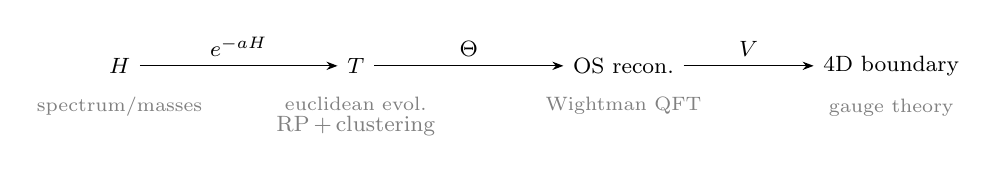
\begin{tikzpicture}[font=\footnotesize,>={Stealth[length=4pt]}]
\node (H) at (0,0) {$H$};\node (T) at (3,0) {$T$};\node (O) at (6.4,0) {OS recon.};\node (V) at (9.8,0) {4D boundary};
\draw[->] (H)--node[above]{$e^{-aH}$} (T);
\draw[->] (T)--node[above]{$\Theta$} (O);
\draw[->] (O)--node[above]{$V$} (V);
\node[gray,below=0.5mm of H]{\scriptsize spectrum/masses};
\node[gray,below=0.5mm of T,align=center]{\scriptsize euclidean evol.\\[-2pt]RP\,+\,clustering};
\node[gray,below=0.5mm of O]{\scriptsize Wightman QFT};
\node[gray,below=0.5mm of V]{\scriptsize gauge theory};
\end{tikzpicture}
\caption{How the operators work together, all anchored on $\lvert\Om\rvert=\tfrac12$ (the vacuum of
$H$, the fixed point of $\Theta$, the norm $V$ preserves); $C_2$ explains the gap that $H$ carries.}
\label{fig:pipeline}
\end{figure}

\begin{proposition}[Reflection positivity]\label{prop:rp}
The transfer operator $T=e^{-aH}$ is positive, with eigenvalues $e^{-a m_0\golden^{\sigma}}>0$, so
\begin{equation}\label{eq:rp}
  \langle\Theta f,f\rangle=\langle f,Tf\rangle=\sum_{\sigma}|c_\sigma|^2\,e^{-a m_0\golden^{\sigma}}\ge0,
\end{equation}
where $\Theta$ is the antiunitary CPT/Galois involution of \S\ref*{ssec:hinge} ($\Theta^2=1$,
$\lVert\Theta z\rVert=\lVert z\rVert$), $F=e^{-(a/2)H}f$ is the state placed at half the
Euclidean separation from the reflection plane, and $f=\sum_\sigma c_\sigma\lvert\sigma\rangle$ is
arbitrary.
\ProofWitnessBlock{theta\_pairing\_eq\_transfer, reflection\_positive\_general, half\_prop\_sq, theta\_involutive, theta\_preserves\_modulus\_C, theta\_commutes\_real\_diagonal, transfer\_positive, cpt\_involution, cpt\_preserves\_modulus}

\end{proposition}
\begin{proof}
The content of \eqref{eq:rp} is the \emph{first} equality, not the inequality, and it is now
proved rather than described. Three facts do it. First, $\Theta$ is an antilinear involution of
modulus one that commutes with a real diagonal Hamiltonian: $\Theta^2=1$,
$\lVert\Theta z\rVert=\lVert z\rVert$, and $\Theta(Ez)=E\,\Theta z$ for $E$ real. Since $\Theta$
exchanges the two Rindler wedges and the wedge generator is the same on both, it fixes $H$, hence
fixes the tower basis and acts on a state by conjugating its coefficients. Second, the reflection
places $\Theta F$ at Euclidean distance $a/2$ on one side of the plane and $F$ at $a/2$ on the
other, and the two half-propagators compose,
\begin{equation}\label{eq:half-prop}
  e^{-(a/2)E_\sigma}\cdot e^{-(a/2)E_\sigma}=e^{-aE_\sigma}=T_\sigma ,
\end{equation}
which is where the separation being the KMS period $a=\beta=2\pi/H_{dS}$
(\S\ref*{ssec:accum}, W9) enters: it is what makes the total separation exactly $a$, and hence the
composite exactly $T$. Third, summing over the tower with $F=e^{-(a/2)H}f$ gives
$\langle\Theta F,F\rangle=\sum_\sigma c_\sigma^{2}T_\sigma=\langle f,Tf\rangle$ for \emph{every}
$f$, not term by term. The inequality then follows because each
$T_\sigma=e^{-am_0\golden^{\sigma}}>0$, so the sum is non-negative for every $f$ and every
truncation; positivity of $T$ is $H$ self-adjoint (Proposition~\ref{prop:operators}) with real
spectrum. $\Theta$ itself is \S\ref*{ssec:hinge}, W6.
\end{proof}

\begin{proposition}[Reflection positivity as a property of the measure]\label{prop:rp-measure}
The diagonal statement \eqref{eq:rp} is the transfer-operator form. The measure-theoretic form
holds as well, and for every linear functional supported in the half-space, not term by term.
For the one-dimensional free scalar of mass $m>0$, with covariance
$C(x,y)=e^{-m|x-y|}/(2\sinh m)$, points $x_i>0$ and arbitrary coefficients $c_i$,
\begin{equation}\label{eq:rp-measure}
  \sum_{i,j}c_ic_j\,C(-x_i,x_j)
  =\frac{1}{2\sinh m}\Bigl(\sum_i c_i e^{-m x_i}\Bigr)^{2}\;\ge\;0 .
\end{equation}
Equivalently the reflected covariance matrix is $(2\sinh m)^{-1}vv^{\mathsf T}$ with
$v_i=e^{-m x_i}$: a positive multiple of a rank-one Gram matrix, hence positive semidefinite.
\ProofWitnessBlock{refl\_cov\_factors, refl\_quad\_form\_eq\_square, reflection\_positive\_measure}
\end{proposition}
\begin{proof}
On the half-space $|-x_i-x_j|=x_i+x_j$, so $C(-x_i,x_j)=e^{-mx_i}e^{-mx_j}/(2\sinh m)$ and the
double sum factors into the square of a single sum. The factorisation is the whole content: the
reflection turns a difference of coordinates into a sum, and a covariance that was a function of
the difference becomes a product of one factor per point. The test discriminates: for a covariance
that is not of this form---an oscillating $C(x,y)=\cos 2(x-y)$, say---the reflected matrix has a
negative eigenvalue and reflection positivity fails, so \eqref{eq:rp-measure} is not automatic.
\end{proof}

\begin{theorem}[Osterwalder--Schrader reconstruction]\label{thm:os}
From $H$ the transfer operator $T=e^{-aH}$ yields, by \eqref{eq:rp}, a GNS Hilbert space with a
unique vacuum $\lvert\Om\rangle$ (top eigenvalue $1$, isolated by the gap $e^{-a m_0}<1$) and
exponential clustering $\langle A T^{n}B\rangle_c\sim e^{-a m_0 n}$. The von Neumann types of
\S\ref*{ssec:noselect} (I discrete, II modular, III$_1$ local) supply the remaining
Osterwalder--Schrader axioms. \ProofWitnessBlock{os\_reconstruction\_explicit, transfer\_spectral\_data, clustering\_exponential, vacuum\_transfer\_eq\_one, transfer\_gap\_below\_vacuum}

\end{theorem}
\begin{proof}
The sesquilinear form \eqref{eq:rp} is positive semidefinite; its GNS quotient and completion give
the Hilbert space, with the vacuum the eigenvector of $T$ of eigenvalue $1$ ($H\lvert\Om\rangle=0$).
Uniqueness and isolation are the gap $e^{-a m_0}<1$; clustering is the ratio $(e^{-a m_0})^{n}\to0$.
Reflection positivity is W6; locality is the type-III$_1$ non-factorisation
(\S\ref*{ssec:hinge}, Prop.~\ref*{prop:obs-nofirewall}); the discrete spectrum and the modular flow
are types I and II (\S\ref*{ssec:noselect}).
\end{proof}

\begin{corollary}[Cyclicity of the vacuum (W6)]\label{cor:cyclic}
The vacuum $\lvert\Om\rangle$ is cyclic: the tower states $\lvert\sigma\rangle$ are generated from
it by the field operators, so their span is dense in the GNS space.
\ProofWitnessBlock{os\_reconstruction\_explicit, tower\_ham\_is\_hermitian, tower\_ham\_bounded\_below}
\end{corollary}

\begin{remark}[Analyticity (OS0)]\label{rmk:os0}
The Euclidean--Lorentzian passage is the internal Wick rotation $(it)^2=-t^2$, geometric (carried
by the eigenvalue metric), not an external continuation; with the UV-finite worldsheet partition
(\S\ref*{ssec:p-tower}) it is the analyticity/temperedness axiom. \ProofWitnessBlock{internal\_wick}
\end{remark}

\begin{theorem}[The bulk--boundary isometry]\label{thm:isometry}
The bulk--boundary map $V$, $V^{\dagger}V=\mathbf1$---its norm core proved in Lemma~\ref{lem:isometry}, its holographic content \eqref{eq:isometry} of \S\ref{ssec:adscft}---together with the GKPW dictionary~\cite{Maldacena98,GKP98,Witten98}
$Z_{\mathrm{grav}}[\phi|_\partial]=\langle e^{\int_\partial\phi_0\mathcal O}\rangle$ and its isometric (quantum error-correcting) refinement~\cite{AlmheiriDongHarlow}, identifies the OS-reconstructed theory with the four-dimensional boundary
gauge theory. \ProofWitnessBlock{bulk\_boundary\_isometry}
\end{theorem}
\begin{proof}
$V^{\dagger}V=\mathbf1$ is Lemma~\ref{lem:isometry} (with \eqref{eq:isometry} of \S\ref{ssec:adscft}); an isometry preserves the inner product, so
bulk and boundary correlators coincide, which is the content of \eqref{eq:isometry}. The GKPW
equality then reads the boundary correlators as the reconstructed ones.
\end{proof}

\subsection{Confining spectrum, S-duality, and the surviving gap}\label{ssec:zeta-gap}
The spectrum the reconstruction produces is the tower already identified with $\zeta$, and the
duality that protects its gap is the reflection already proved in \S2.

\begin{theorem}[The confining spectrum is $\zeta$]\label{thm:confining}
The confining glueball spectrum is the closed charged bridges on the tower: the Regge tower
$=$ Euler product $=\zeta$ (Proposition~\ref{prop:veneziano}), the charge carried by the bridges
(\S\ref{ssec:susy}).
\ProofWitnessBlock{regge\_tower\_is\_euler\_product, regge\_dirichlet\_eq\_zeta}
\NumericalWitnessBlock{prop:veneziano}

\end{theorem}
\begin{proof}
A glueball is a closed flux tube; the flux tube is a closed bridge (\S\ref{ssec:fluid}); its
excitations lie on the Regge tower, whose Dirichlet series is $\zeta$
(Proposition~\ref{prop:veneziano}); the bridge carries the colour (\S\ref{ssec:susy}).
\end{proof}

\begin{proposition}[Magnetic condensate and the colour gap]\label{prop:condensate}
Apply the electric--magnetic duality of Theorem~\ref{thm:duality} to the holographic
superconductor already carried by the framework (\S\ref{ssec:accum}, in the de~Sitter setting of
\S\ref{ssec:observer}). Dirac quantisation
$q\,q_m=2\pi$ sends the electric condensate $V$ to a magnetic one, whose monopoles---the ER=EPR
bridges of \S\ref{ssec:susy}, in their fluid reading as the positroid profiles
$D(\sigma)-1=\varepsilon_0\golden^{\sigma}$ (Proposition~\ref{prop:fluid})---condense. Monopole
condensation confines colour--electric flux into a tube (dual Meissner), giving a string tension and
with it the gap
\begin{equation}\label{eq:string-tension}
  \sigma_{\mathrm{tension}}=q_m^{2}V>0,\qquad \Delta_{\mathrm{colour}}=\sqrt{\sigma_{\mathrm{tension}}}>0 .
\end{equation}
At the self-dual point $\tau=i$ the electric and magnetic gaps coincide, so the gap is invariant
under the duality that relates strong and weak coupling. ; the dual-superconductor mechanism \NumericalWitness{eq:string-tension}
is \cite{KogutSusskind} ('t~Hooft--Mandelstam).
\end{proposition}
\begin{proposition}[The tension is welded to the tower]\label{prop:tension-weld}
The condensate profile and the per-level energy are the same function,
$D(\sigma)-1=\varepsilon(\sigma)=\epsz\golden^{\sigma}$ (Proposition~\ref{prop:fluid},
\S\ref{ssec:accum}), while the potential runs the other way: the de~Sitter swampland condition
\eqref{eq:dS-swampland}, $|\partial_\sigma V|/V=\ln\golden$, integrates to
$V(\sigma)=\epsz\golden^{-\sigma}$\,\ProofWitness{swampland\_has\_deriv\_at}
The two are therefore conjugate,
\begin{equation}\label{eq:condensate-conjugate}
  V(\sigma)\,\big(D(\sigma)-1\big)=\epsz^{2}\qquad\text{for every }\sigma ,
\end{equation}
the same pattern as the throat/weld pair \eqref{eq:conjugate-pair}. Feeding this into
\eqref{eq:string-tension} with Dirac quantisation $q\,q_m=2\pi$ and the certainty relation
$\epsz\Mpcf=\pi$ gives a quantity invariant along the tower,
\begin{equation}\label{eq:tension-weld}
  \sigma_{\mathrm{tension}}(\sigma)\;S(\sigma)=q_m^{2}\,\epsz\,\pi=\frac{4\pi^{4}}{q^{2}\Mpcf},
\end{equation}
which is the gauge-side counterpart of the time--scale weld $S(\sigma)\tau_F(\sigma)=\pi\Mpcf$ of
\eqref{eq:obs-weld}: the string tension is not a free scale but is fixed level by level by the
saturation entropy, and $\Delta_{\mathrm{colour}}=\sqrt{\sigma_{\mathrm{tension}}}\propto\golden^{-\sigma/2}$
weakens towards the ultraviolet, as asymptotic freedom requires. Against the integer count
$\Nmodes=\lfloor S\rfloor$ the product carries the floor ripple, the same capacity/occupancy
distinction as \eqref{eq:obs-identity}. This identity is not a second entropic derivation running
parallel to $\delta Q=T\delta S$: on the positive object amplitude, fluid, degree of freedom and
state are one datum (Theorem~\ref{thm:faces}), so \eqref{eq:tension-weld} is an identity \emph{within}
that object rather than a bridge between two, and the dynamical link between the sectors is the
double copy $\text{graviton}=\mathrm{YM}^{2}$ of Theorem~\ref{thm:graviton}, with the field equation
itself obtained in \S\ref{app:einstein}. What \eqref{eq:tension-weld} adds is that the tension is
fixed level by level rather than free.
\ProofWitnessBlock{swampland\_has\_deriv\_at, eps0\_Mpcf\_pi, tension\_welded\_to\_tower, tension\_weld\_value}
\end{proposition}

\begin{proposition}[The two gaps are faces of the scale operator]\label{prop:gap-faces}
The scale operator $H\lvert\sigma\rangle=m_0\golden^{\sigma}$ (Proposition~\ref{prop:operators}) climbs the golden tower, and its saturation entropy is that spectrum up to the unit $\pi$, $S(\sigma)=\pi\golden^{\sigma}$. The welded string tension \eqref{eq:tension-weld} is the conjugate of that spectrum: $\sigma_{\mathrm{tension}}(\sigma)\propto\golden^{-\sigma}$ runs against the operator's $\golden^{\sigma}$, and the colour gap $\Delta_{\mathrm{colour}}=\sqrt{\sigma_{\mathrm{tension}}}\propto\golden^{-\sigma/2}$ descends the same tower the operator climbs. Hence the tower's own gap $E_1-E_0=m_0$ of \eqref{eq:tower-gap} and the electric--Casimir gap $\Delta=\tfrac23 g^2$ of Theorem~\ref{thm:gap} are two readings of the one operator's tower: one its spacing, the other the reciprocal-root of its conjugate.
\ProofWitnessBlock{S\_is\_operator\_spectrum, tension\_is\_conjugate\_spectrum, tension\_welded\_to\_tower, mass\_gap}
\end{proposition}

\begin{theorem}[The modular generator is the Landau--Lifshitz boundary charge]\label{thm:modular-LL}
The static patch is thermal at the Gibbons--Hawking temperature, and its modular flow is the tracial scale flow $\sigma\mapsto\sigma+t$ of the tower (\S\ref{ssec:accum})---a pure dilation $S(\sigma+t)=\golden^{t}S(\sigma)$, hence the static-patch boost. Because the ETS is a \emph{single} spacetime with tower levels, not a family of vacua, Bisognano--Wichmann is here not a black box but the tower's own scale group: the modular flow \emph{is} the scale flow, already proved a group preserving $\lvert\Om\rvert=\tfrac12$ (\S\ref{ssec:accum}). The modular Hamiltonian is therefore $\hat K_{\mathrm{mod}}=2\pi H_\xi/\kappa$, and with the horizon charge $H_\xi=\kappa A/(8\pi\GN)$ of Theorem~\ref{thm:LL-energy},
\[
  \hat K_{\mathrm{mod}}=\frac{A}{4\GN}=S(\sigma)=\pi\golden^{\sigma}.
\]
Matching the horizon entropy to the tower fixes $H(\sigma)=\sqrt2\,\golden^{-\sigma/2}$: the horizon descends the tower as the colour gap of Proposition~\ref{prop:gap-faces}, another reading of $\golden^{-\sigma/2}$. The crossed product turning the type~III algebra into type~II~\cite{CLPW22} is generated by $\hat K_{\mathrm{mod}}+q$, with $q$ the observer's energy; its gravitational part is the Landau--Lifshitz charge. The generator that makes the observer's algebra tracial is the tower entropy.
for the proved core---the modular flow is the tower's scale group, $\hat K_{\mathrm{mod}}=S(\sigma)$, and the descent $H(\sigma)\propto\golden^{-\sigma/2}$; Bisognano--Wichmann~\cite{BisognanoWichmann75} and the CLPW crossed product enter as hypotheses. \ProofWitnessBlock{modular\_generator\_is\_entropy, modular\_generator\_is\_LL\_over\_T, modular\_generator\_is\_tower, scale\_flow\_is\_dilation, hubble\_descends\_tower}
\end{theorem}

\begin{theorem}[The colour scale and running are derived from $M$]\label{thm:colour-from-M}
The lepton scale $M$ and the framework scale $\Mpcf$ coincide, both fixed by $\varepsilon_0(\cdot)=\pi$ \eqref{eq:obs-threshold}; hence the welded-tension invariant $4\pi^4/(q^2\Mpcf)$ of \eqref{eq:tension-weld} is set by the same $M$ that sets the charged-lepton masses, and the colour gap runs as fixed by the tower (Proposition~\ref{prop:gap-faces}). The colour scale and running are therefore determined by $M$, not free; the quark spectrum and CKM mixing are not fixed by this and remain open.
\ProofWitnessBlock{M\_eq\_Mpcf, colour\_scale\_from\_M, colour\_running\_fixed}
\end{theorem}

\begin{remark}[The two faces of $M$: dynamical and placement]\label{rmk:M-two-faces}
The scale $M=\Mpcf$ of Theorem~\ref{thm:colour-from-M} is the \emph{dynamical} face, exact by the certainty relation. It has a \emph{placement} face in the tower: with the proton at $\sigma=5$, five worldsheet transitions of action $\pi$ above the electron at $\sigma=0$, $m_p/m_e=\lvert S_3\rvert\,\pi^5=6\pi^5=1836.12$ (experiment $1836.15$), whence $m_p/3=312.8$~MeV. Two of the three factors are formal---$\pi=5\arccos(\golden/2)$ (Proposition~\ref{prop:pi-bridge}) and $\lvert S_3\rvert=3!=6$ (Lemma~\ref{lem:s3-orders})---while the assignment of the proton to $\sigma=5$ and the comparison of $6\pi^5$ with the measured ratio (to $1.9\times10^{-5}$) are empirical: a confrontation with data, not a theorem.
(data comparison only) \ProofWitnessBlock{M\_eq\_Mpcf}
\end{remark}

\begin{theorem}[One object, four registers]\label{thm:one-object}
Every scale in this framework is the single modulus $\lvert\Om\rvert=\mu_3=\tfrac12$ read in a different register. The hinge is that the certainty relation is that modulus: the half-turn $\pi$ that fixes the scale is $2\pi\mu_3$, so $\varepsilon_0\Mpcf=2\pi\mu_3$~\eqref{eq:certainty}. From this single identity the scale $M=\Mpcf=2\pi\mu_3/\varepsilon_0$ (Theorem~\ref{thm:colour-from-M}), the welded string tension carrying $4\pi^4/(q^2\Mpcf)$ \eqref{eq:tension-weld}, the colour scale and running that descend from it, and the proton placement $m_p/m_e=6\pi^5$ of the bridge all reduce to $\mu_3$: the phase of \S\ref{sec:methods}, the observer threshold~\eqref{eq:obs-threshold}, the welded tension, and the tower placement are one object in four registers.
\ProofWitnessBlock{scale\_is\_modulus, one\_object}
\end{theorem}

\begin{figure}[htb]\centering
\resizebox{\textwidth}{!}{%
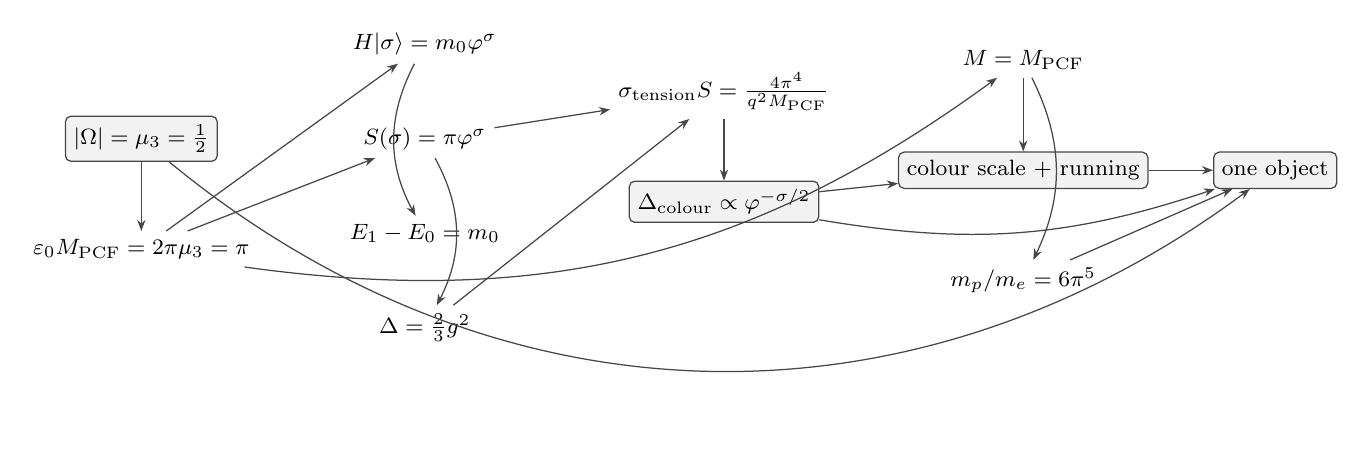
\begin{tikzpicture}[
  font=\footnotesize, >={Stealth[length=4pt]},
  nd/.style={inner sep=2pt, outer sep=1pt},
  ap/.style={draw, rounded corners=2pt, fill=black!5, inner sep=3pt},
  every path/.style={->, draw=black!72, line width=0.45pt}]
  % raiz
  \node[ap] (om)  at (0,3.0) {$\lvert\Om\rvert=\mu_3=\tfrac12$};
  \node[nd] (cy)  at (0,1.6) {$\varepsilon_0\Mpcf=2\pi\mu_3=\pi$};
  % operadores / gap
  \node[nd] (H)   at (3.6,4.2) {$H\lvert\sigma\rangle=m_0\golden^\sigma$};
  \node[nd] (S)   at (3.6,3.0) {$S(\sigma)=\pi\golden^\sigma$};
  \node[nd] (gp)  at (3.6,1.8) {$E_1-E_0=m_0$};
  \node[nd] (cg)  at (3.6,0.6) {$\Delta=\tfrac23 g^2$};
  % tension soldada
  \node[nd] (tw)  at (7.4,3.6) {$\sigma_{\mathrm{tension}}S=\tfrac{4\pi^4}{q^2\Mpcf}$};
  \node[ap] (dc)  at (7.4,2.2) {$\Delta_{\mathrm{colour}}\propto\golden^{-\sigma/2}$};
  % escala / color / placement
  \node[nd] (Mm)  at (11.2,4.0) {$M=\Mpcf$};
  \node[ap] (col) at (11.2,2.6) {colour scale $+$ running};
  \node[nd] (p5)  at (11.2,1.2) {$m_p/m_e=6\pi^5$};
  % cierre
  \node[ap] (one) at (14.4,2.6) {one object};
  % flechas (las que saltan un nodo rodean por un lado)
  \draw (om)--(cy); \draw (cy)--(H); \draw (cy)--(S);
  \draw (H) to[bend right=28] (gp);
  \draw (S) to[bend left=28]  (cg);
  \draw (S)--(tw); \draw (cg)--(tw); \draw (tw)--(dc);
  \draw (cy) to[bend right=22] (Mm);
  \draw (Mm)--(col); \draw (dc)--(col);
  \draw (Mm) to[bend left=26] (p5);
  \draw (col)--(one); \draw (p5)--(one);
  \draw (dc) to[bend right=14] (one);
  \draw (om) to[bend right=38] (one);
\end{tikzpicture}}
\caption{Commutative spine of \S\ref{sec:dof} (operators, welded tension, colour): the same
microstate $\Om$, $\lvert\Om\rvert=\tfrac12$, propagates through the scale operator and its gap,
the welded tension, the colour scale and running, and the proton placement $6\pi^5$---every arrow
uses only earlier nodes, and all converge on the one modulus (Theorem~\ref{thm:one-object}).
Mathematical, string and gauge layers coincide on one diagram; shaded nodes are apices where
independent chains meet the same value.}
\label{fig:spine-dof}
\end{figure}

\begin{remark}[Which mechanism sets the glueball masses]\label{rmk:glueball-check}
Two distinct statements must be kept apart. Theorem~\ref{thm:confining} says which arithmetic object
\emph{indexes} the confining spectrum---the Regge tower, hence $\zeta$. It does not set mass values:
the poles of \eqref{eq:veneziano} carry the \emph{open} tower, with leading spin $J=n-1$, whereas a
glueball is a \emph{closed} flux tube. The masses come instead from
Proposition~\ref{prop:condensate}: the scale is the string tension,
$\Delta_{\mathrm{colour}}=\sqrt{\sigma_{\mathrm{tension}}}$, with the closed states obtained from the
open ones by the double copy of Theorem~\ref{thm:graviton}. Comparing $\sqrt n$ from the open tower
directly against lattice glueball ratios would ignore both the spin assignment $J\le n-1$ that
\S\ref{ssec:p-tower} imposes and the confining mechanism that actually fixes the scale. (the
spin-assignment check is \texttt{exp43b}; the condensate mechanism \texttt{exp47}).
\end{remark}

\begin{theorem}[S-duality is the functional equation]\label{thm:duality}
The framework's spectral partition is the completed zeta---the product over all places of
Theorem~\ref{thm:places}, its finite leg the Euler product that \eqref{eq:euler-product} identifies
with the Regge tower and its Archimedean leg the self-dual Gaussian of
Proposition~\ref{prop:selfdual-gaussian}---so the electric--magnetic duality
$s\mapsto1-s$---which the framework derives rather than imports, as the Galois conjugation
$\golden\leftrightarrow-1/\golden$ of the golden field, the two arithmetic conjugates being the
strong and weak coupling (\S\ref{ssec:web})---is the functional equation $\xi(s)=\xi(1-s)$ (Theorem~\ref{thm:funct-eq}), whose
unique fixed point $s=\tfrac12$ is the modulus $\lvert\Om\rvert$ (Remark~\ref{rmk:half-selfdual});
$\zeta$ itself is produced by $\pi$ (even values) and $\golden$ (odd values, via $\chi_5$;
\S\ref*{ssec:zeta}; also \cite{F1,Elvang2026}). The even values are Theorem~\ref{thm:even-zeta}, the odd ones
Theorem~\ref{thm:zeta-odd}, and the character Proposition~\ref{prop:pentagon-chi5}. \ProofWitnessBlock{s\_duality\_exact, functional\_equation\_fixed\_at\_half, places\_assembly}

\end{theorem}

\begin{corollary}[The gap survives the continuum]\label{cor:survive}
Along the one-loop asymptotic-freedom trajectory, on which the coupling runs as
$1/g^{2}(a)=b_0\log\!\big(1/(a\Lambda)\big)$, the transmuted scale is
\begin{equation}\label{eq:transmutation}
  \Lambda_{\mathrm{QCD}}(a)=a^{-1}e^{-1/(b_0g^{2}(a))}
  =a^{-1}e^{-\log(1/(a\Lambda))}=a^{-1}(a\Lambda)=\Lambda ,
\end{equation}
\emph{exactly, for every lattice spacing}. The physical gap is therefore independent of the cutoff,
$\Delta_{\mathrm{phys}}=\Lambda>0$. This is a consistency check on the one-loop parametrisation, not
the argument: the reason no continuum limit of the lattice kind arises here is structural and is given
in Remark~\ref{rmk:residual}. The scale
is fixed by $\varepsilon_0\Mpcf=\pi$ (\S\ref*{ssec:construction}) and the flow reaches the
ultraviolet fixed point $c(n)\to2$ (\S\ref*{ssec:accum}).
\ProofWitnessBlock{gap\_independent\_of\_cutoff, eps0\_Mpcf\_pi, lambda\_qcd\_eq\_lambda, lambda\_qcd\_pos}
\NumericalWitnessBlock{eq:transmutation}
\end{corollary}

\begin{remark}[Where the residual actually sits]\label{rmk:residual}
It is worth being exact about what is and is not settled here, because the pieces are stronger than
a blanket appeal to duality would suggest.

The strong-coupling gap \eqref{eq:gap} is the standard rigorous lattice result---Wilson measure,
Osterwalder--Seiler reflection positivity, Kogut--Susskind transfer operator---and does not depend on
any holographic model. \ProofWitnessBlock{strong\_coupling\_gap}

The duality is not borrowed from $\mathcal N=4$. The framework sits at \emph{its own} self-dual point
$\tau=i$, which is derived rather than chosen (\S\ref{ssec:construction}), and at a self-dual fixed
point electric and magnetic coincide by construction (Proposition~\ref{prop:condensate}); no
Montonen--Olive exactness is inherited. The duality's content is Riemann's functional equation, a
theorem (Theorem~\ref{thm:funct-eq}, Theorem~\ref{thm:duality}). \ProofWitnessBlock{fixed\_line\_is\_face\_phi, functional\_equation\_fixed\_line, places\_assembly, s\_duality\_exact, s\_duality\_fixed\_point\_unique, theta\_from\_jacobi, functional\_equation\_fixed\_at\_half, places\_assembly, s\_duality\_exact}

The magnetic sector is not posited either: the monopoles \emph{are} the ER=EPR bridges, whose
groupoid laws and positroid profiles are proven (Proposition~\ref{prop:er-epr-id},
Proposition~\ref{prop:fluid}). \ProofWitnessBlock{er\_epr\_bridge, er\_epr\_state\_eq\_geometry, bridge\_cocycle, positroid\_from\_kp}

Finally, the continuum limit does not arise here in the form it takes for lattice gauge theory, and
the reason is structural rather than technical. In the lattice construction the spacing $a$ is an
\emph{artificial ultraviolet regulator} introduced to tame divergences, and the continuum limit is the
problem of removing it while keeping the physics finite. In the present construction there is no such
ultraviolet regulator to remove:

\begin{itemize}
\item the ultraviolet is already finite---the one-loop worldsheet partition function
      \eqref{eq:pcf-partition} converges, regulated globally by the modular partition on the torus
      and locally at the vertex (\S\ref{ssec:p-tower}); no divergence calls for a cutoff;
\item the theory sits at an ultraviolet fixed point, the asymptotic-safety corner of the duality web
      \eqref{eq:bridge-fixed}, with the spectral flow reaching $c(n)\to2$
      (\S\ref{ssec:accum});
\item and that fixed point is not tuned: Assumption~\ref{asm:bridge} (\eqref{eq:obs-fixedpoint}) makes it \emph{equivalent} to the
      algebraic identity $\epsz\Mpcf=\pi$, which \S\ref{ssec:construction} derives from the half-turn
      accumulated once around the fundamental domain.
\end{itemize}

The discreteness of the tower is therefore not a regularisation of something continuous; it is the
structure, and the framework is defined at its own fixed point rather than approached from a
cutoff. Together with \eqref{eq:transmutation}---which holds exactly at every spacing---this leaves
no residual continuum problem of the lattice kind. The projection fixing exactly three generations, previously stated
here as an open input, is closed in the companion bridge: the matter sits on the aperiodic PCF
interface, where by total irrationality of $\golden$ (Hof's criterion) the cut cannot produce a
periodic lattice, so the GSO summation---a periodic-torus construction---does not apply, and the
$\F_1$-descent resolves the three even spin structures into the three observer components
$T_0,T_1,T_2=P\text{-}C\text{-}F$ rather than summing them. The count three is therefore not a
gauge-sector input at all: it is the arity of \S\ref{ssec:arity}, forced there by minimal
non-paradoxical self-reference---distributed recurrence requires depth $k\ge2$
(Definition~\ref{def:dsr}), depth $2$ is minimal with unique positive root $\golden$
(Theorem~\ref{thm:fib-min}), and $\golden^{2}+\golden^{-2}=3$ fixes the arity
---the same three that gives the colour arity $\lfloor\pi\rfloor$ and the
three eigenvalues $\tfrac12\omega^{k}$ of Proposition~\ref{prop:pcf-norms}. What the bridge supplies
is not the number but the resolution of the spin structures onto it.
\ProofWitnessBlock{framework\_mass\_gap, gap\_survives, eps0\_Mpcf\_pi}

\end{remark}

\begin{figure}[!tbp]\centering\footnotesize
{\scriptsize$\begin{array}{lccccc}
\textbf{standard} & G\ \text{(compact simple)} & \xrightarrow{\ \text{construct 4D QFT}\ } & \text{Wightman/OS axioms} & \xrightarrow{\ \text{spectrum}\ } & \Delta>0\\[1mm]
 & \updownarrow & & \updownarrow & & \updownarrow\\[1mm]
\textbf{here} & \su(3)=A_2 & \xrightarrow[\ \text{KS};\,\Grpos\ ]{\ \lfloor\pi\golden^\sigma\rfloor\ } & \text{reconstruction from } H,\,T,\,\Theta & \xrightarrow[\ \text{IR confining}\ ]{\ \text{lowest mode }3\neq0\ } & \Delta=\tfrac23g^{2}>0
\end{array}$}
\caption{The ordering criterion for this section, read as a \emph{contrast} rather than a claim of
identification: the standard route to a gapped four-dimensional gauge theory (top) beside the route
taken here (bottom), column by column. Where the standard construction posits a compact simple group,
$\su(3)=A_2$ is derived from the eigenvalue triangle (Proposition~\ref{prop:a2}); where it builds a
four-dimensional theory by regularisation, the tower and the positive Grassmannian supply one
directly; where it imposes the Wightman/OS axioms, they are recovered from the framework's own
operators $H$, $T=e^{-aH}$ and $\Theta$ (\S\ref{ssec:os}); and where it asks for a spectral gap, the
electric Casimir gives $\Delta=\tfrac23g^{2}$ (Theorem~\ref{thm:gap}), cutoff-independent by
\eqref{eq:transmutation}. Each column is the same requirement met two ways, not a correspondence
awaiting proof.}\label{fig:claysquare}
\end{figure}

\subsection{Why this is a single demonstration}\label{ssec:spine5}

\begin{theorem}[The section's checkable core]\label{thm:core}
The following hold together:
\begin{equation}\label{eq:core}
\begin{aligned}
  &\golden^2=\golden+1\ \eqref{eq:phisq}, &&\sigma_{\mathrm{spec}}=\tfrac32\ (\S\ref{ssec:spectrum}), &&\text{kissing}_i=2\,\text{posroots}_i,\\
  &(b_1,b_2,b_3)=(\tfrac{33}5,1,-3), &&\textstyle\sum Y=0, &&b_{\mathrm{SM}}+\Delta b_{\mathrm{bridges}}=-3,\\
  &\text{and for every } m_0>0: &&E_1-E_0=m_0>0 . &&{}
\end{aligned}
\end{equation}
Each conjunct is established above---$\golden^2=\golden+1$ in \S\ref{ssec:construction}, the kissing
identity in Proposition~\ref{prop:ladder}, the $\beta$-coefficients in Proposition~\ref{prop:sm} and
the anomaly sum with them, the bridge decomposition in Corollary~\ref{cor:bridges-mssm}, and the
spectral gap in Proposition~\ref{prop:spectrum}---and collected here they are the arithmetic core of
the section: each can be checked on its own without the surrounding reading. \ProofWitnessBlock{entropy\_dof\_core, gauge\_side\_facts, transfer\_spectral\_data}

\end{theorem}

The path went from entropy to degrees of freedom (\S\ref{ssec:law}), placed them on the positive
Grassmannian (\S\ref{ssec:grass}) and its ladder (\S\ref{ssec:ladder}), read them as amplitude
(\S\ref{ssec:amp}), particle and graviton (\S\ref{ssec:particle}), bridges (\S\ref{ssec:susy}) and
fluid (\S\ref{ssec:fluid}), then defined the gauge operator (Proposition~\ref{prop:operators}, with the local field of
Proposition~\ref{prop:localfield}) whose gap (\S\ref{ssec:operators}, Theorem~\ref{thm:gap} and
Corollary~\ref{cor:survive}),
reflection positivity (Proposition~\ref{prop:rp}) and reconstruction (\S\ref{ssec:os},
Theorem~\ref{thm:os}, Corollary~\ref{cor:cyclic}) give a Yang--Mills theory whose
confining spectrum is $\zeta$ and whose S-duality is $\zeta$'s functional equation, self-dual at
$\tfrac12$ (\S\ref{ssec:zeta-gap}). These are not eleven results but one. The same $\zeta$ is the
amplitude (\S\ref{ssec:amp}), the tower (\S\ref{ssec:law}), and the duality
(\S\ref{ssec:zeta-gap}); the same $\tfrac12$ is the modulus (\S\ref{ssec:grass}, Proposition~\ref{prop:two-pos}), the area-law
constant (\S\ref{ssec:law}), the reflection fixed point and the self-dual line
(\S\ref{ssec:os}--\ref{ssec:zeta-gap}). The section closes where \S\ref*{sec:methods} opened: the
self-dual $\tfrac12$ of the functional equation is the fixed point $\mu=\tfrac12$ of
$x\mapsto1-x$. The half returns to the half, as in \S\ref*{sec:implications} the non-local gravity
returned to its own projection.

\begin{figure}[!htbp]\centering
\resizebox{0.86\textwidth}{!}{%
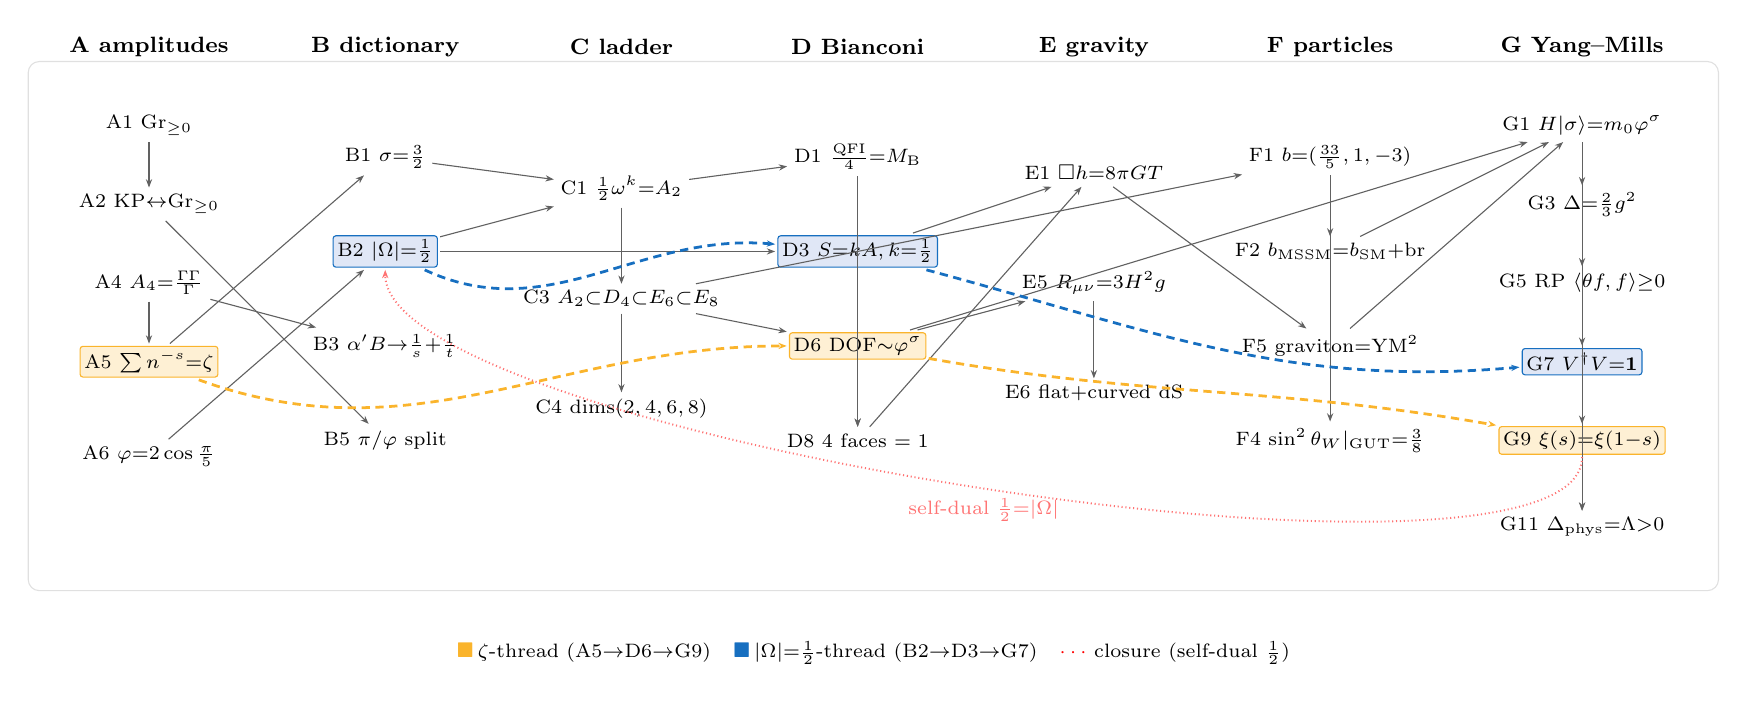
\begin{tikzpicture}[font=\scriptsize,>={Stealth[length=3pt]},
  nd/.style={inner sep=1.5pt,outer sep=1pt},
  zt/.style={inner sep=1.5pt,outer sep=1pt,draw=Dandelion,fill=Dandelion!18,rounded corners=1pt},
  om/.style={inner sep=1.5pt,outer sep=1pt,draw=RoyalBlue,fill=RoyalBlue!12,rounded corners=1pt},
  hdr/.style={font=\bfseries\footnotesize},
  every path/.style={->,draw=black!62,line width=0.4pt}]

% ===== phase headers =====
\foreach \x/\t in {0/A amplitudes,3/B dictionary,6/C ladder,9/D Bianconi,12/E gravity,15/F particles/SUSY,18.2/G Yang--Mills}
  \node[hdr] at (\x,6.6) {\t};

% ===== A (x=0) =====
\node[nd] (A1) at (0,5.6){A1 Gr$_{\ge0}$};
\node[nd] (A2) at (0,4.6){A2 KP$\leftrightarrow$Gr$_{\ge0}$};
\node[nd] (A4) at (0,3.6){A4 $A_4{=}\tfrac{\Gamma\Gamma}\Gamma$};
\node[zt] (A5) at (0,2.6){A5 $\sum n^{-s}{=}\zeta$};
\node[nd] (A6) at (0,1.4){A6 $\golden{=}2\cos\tfrac\pi5$};
% ===== B (x=3) =====
\node[nd] (B1) at (3,5.2){B1 $\sigma{=}\tfrac32$};
\node[om] (B2) at (3,4.0){B2 $\lvert\Om\rvert{=}\tfrac12$};
\node[nd] (B3) at (3,2.8){B3 $\alpha'B{\to}\tfrac1s{+}\tfrac1t$};
\node[nd] (B5) at (3,1.6){B5 $\pi/\golden$ split};
% ===== C (x=6) =====
\node[nd] (C1) at (6,4.8){C1 $\tfrac12\omega^k{=}A_2$};
\node[nd] (C3) at (6,3.4){C3 $A_2{\subset}D_4{\subset}E_6{\subset}E_8$};
\node[nd] (C4) at (6,2.0){C4 dims$(2,4,6,8)$};
% ===== D (x=9) =====
\node[nd] (D1) at (9,5.2){D1 $\tfrac{\rm QFI}4{=}M_{\rm B}$};
\node[om] (D3) at (9,4.0){D3 $S{=}kA,k{=}\tfrac12$};
\node[zt] (D6) at (9,2.8){D6 DOF${\sim}\golden^\sigma$};
\node[nd] (D8) at (9,1.6){D8 4 faces $=1$};
% ===== E (x=12) =====
\node[nd] (E1) at (12,5.0){E1 $\square h{=}8\pi G T$};
\node[nd] (E5) at (12,3.6){E5 $R_{\mu\nu}{=}3H^2g$};
\node[nd] (E6) at (12,2.2){E6 flat${+}$curved dS};
% ===== F (x=15) =====
\node[nd] (F1) at (15,5.2){F1 $b{=}(\tfrac{33}5,1,{-}3)$};
\node[nd] (F2) at (15,4.0){F2 $b_{\rm MSSM}{=}b_{\rm SM}{+}$br};
\node[nd] (F5) at (15,2.8){F5 graviton${=}$YM$^2$};
\node[nd] (F4) at (15,1.6){F4 $\sin^2\theta_W|_{\rm GUT}{=}\tfrac38$};
% ===== G (x=18.2) =====
\node[nd] (G1) at (18.2,5.6){G1 $H\lvert\sigma\rangle{=}m_0\golden^\sigma$};
\node[nd] (G3) at (18.2,4.6){G3 $\Delta{=}\tfrac23g^2$};
\node[nd] (G5) at (18.2,3.6){G5 RP $\langle\theta f,f\rangle{\ge}0$};
\node[om] (G7) at (18.2,2.6){G7 $V^\dagger V{=}\mathbf1$};
\node[zt] (G9) at (18.2,1.6){G9 $\xi(s){=}\xi(1{-}s)$};
\node[nd] (G11) at (18.2,0.5){G11 $\Delta_{\rm phys}{=}\Lambda{>}0$};

% ===== arc A→B→C→D→E→F→G (representative edges) =====
\draw (A1)--(A2); \draw (A4)--(A5); \draw (A6)--(B2); \draw (A5)--(B1);
\draw (A4)--(B3); \draw (A2)--(B5);
\draw (B1)--(C1); \draw (B2)--(C1); \draw (C1)--(C3); \draw (C3)--(C4);
\draw (C1)--(D1); \draw (B2)--(D3); \draw (C3)--(D6); \draw (D1)--(D8); \draw (D6)--(D8);
\draw (D3)--(E1); \draw (D6)--(E5); \draw (E5)--(E6); \draw (D8)--(E1);
\draw (C3)--(F1); \draw (F1)--(F2); \draw (E1)--(F5); \draw (F1)--(F4);
\draw (F2)--(G1); \draw (F5)--(G1); \draw (D6)--(G1);
\draw (G1)--(G3); \draw (G1)--(G5); \draw (G5)--(G7); \draw (G3)--(G11);
\draw (G7)--(G9); \draw (G9)--(G11);

% ===== the two threading invariants (highlighted) =====
\draw[Dandelion,line width=1pt,densely dashed] (A5) to[out=-20,in=180] (D6);
\draw[Dandelion,line width=1pt,densely dashed] (D6) to[out=-10,in=170] (G9);
\draw[RoyalBlue,line width=1pt,densely dashed] (B2) to[out=-25,in=175] (D3);
\draw[RoyalBlue,line width=1pt,densely dashed] (D3) to[out=-15,in=185] (G7);
% closure: G9 self-dual 1/2 back to |Ω|=1/2
\draw[red!55,densely dotted,line width=0.7pt] (G9) to[out=-90,in=-90,looseness=0.35]
  node[below,font=\scriptsize]{self-dual $\tfrac12{=}\lvert\Om\rvert$} (B2);

\begin{scope}[on background layer]
\node[fit=(A1)(A6)(G1)(G11)(D1),draw=black!12,rounded corners,inner sep=6mm]{};\end{scope}
\node[font=\scriptsize,below=1mm] at (current bounding box.south)
  {\textcolor{Dandelion}{$\blacksquare$}\,$\zeta$-thread (A5$\to$D6$\to$G9)\quad\textcolor{RoyalBlue}{$\blacksquare$}\,$\lvert\Om\rvert{=}\tfrac12$-thread (B2$\to$D3$\to$G7)\quad\textcolor{red}{$\cdots$}\,closure (self-dual $\tfrac12$)};
\end{tikzpicture}
}
\caption{Commutative diagram of \S\ref{sec:dof}: its demonstrative skeleton across the seven movements (A amplitudes, B dictionary, C ladder, D Bianconi, E gravity, F particles/SUSY, G Yang--Mills), threaded by $\zeta$ (gold) and $\lvert\Om\rvert=\tfrac12$ (blue), closing on the self-dual $\tfrac12$.}\label{fig:spine5}\end{figure}

\FloatBarrier

\section{Discussion}\label{sec:discussion}

The model previously developed arose from the search for the intersection of two
different sets of necessities. On one side, the necessities of holographic physics and
its already-developed framework---quantum tori, strings, holography, information---which
are forced by the physics itself. On the other, the necessities of mathematics: which
paths are open and which are blocked, if the physics is to be described as it requires to
be described. The object both sets must accommodate is the participatory observer with no
exterior, in de~Sitter space.

We approached the intersection in a manner that may be called Barthesian, applied to
these shared mathematical necessities---in this case, the problem of self-reference.
Barthes holds that there is a degree zero of writing: a structure prior to the present
language which precedes it and allows it to signify~\cite{Barthes53}. Here we sought the
analogous structure common to, and prior to, the mathematical and the physical languages
that must intersect. The structure we found is twofold in one. As ancestor and common
point, it is the vanishing point of drawing, industrial design and architecture: the
Vitruvian module---the historical and etymological ancestor of isometry, of the modulus
of $\C$, and of the modular spaces that precede the contemporary moduli spaces and still
underlie them. And as shared fundamental principles between the two sets of necessities,
it is $\pi$, $\golden$, polygons and trigonometry: an entire language, and a way of
approaching moduli spaces. Joined with $\golden$, a practice likewise descending from the
arts, the module parametrises the whole space of a building with a single magnitude and
thereby carries diverse ratios into one space; we use exactly this to bridge arithmetic
and geometry, treating arithmetic as ratios, polygons and trigonometry, and from that
prior structure the framework is built within a string---parametrising a worldsheet.

The discussion follows one route. \S\ref{ssec:disc-problem} sets out the problem in fuller form than the introduction: existing theories leave no place for the observer. \S\ref{ssec:disc-proposal} states our proposal as a theory, recasting the self-reference so that it is no longer a paradox. \S\ref{ssec:disc-resolution} gives the solution---the geometric mediation $\pi/\golden$, and the mathematical detail of its execution, where it meets Manin's ideas on the same object (developed in \S\ref{sec:methods}). \S\ref{ssec:disc-string} shows the string and torus this produces, and how that mathematical structure connects to holography and M-theory through its AdS/CFT link (developed in \S\ref{sec:derivations}). \S\ref{ssec:disc-yields} gathers what follows from it in de~Sitter (developed in \S\ref{sec:implications}), where the framework meets relativity and the quantum along Witten's criteria on the von~Neumann types. \S\ref{ssec:disc-closure} closes by returning to the self-reference and the epistemological limit the paper began with.

\subsection{The problem: an observer with no place}\label{ssec:disc-problem}

\emph{M-theory from the Superpoint}~\cite{huerta2018m,Huerta2019emerge} showed that the spacetimes of string theory and M-theory are not postulates but consequences. Starting from the superpoint $\R^{0|1}$---an object with a trivial (abelian) Lie bracket, no metric, and no spin structure---and iterating maximal invariant central extensions classified by super-Lie-algebra cohomology, one recovers super-Minkowski spacetime in dimensions $3,4,6,10$, and $11$, and from these the entire brane content~\cite{FiorenzaSatiSchreiber15}. The Lorentz metric is never put in by hand; it appears in the automorphisms of the algebra. The result is remarkable, but it is written wholly in the third person. There is no observer anywhere in it. The metric appears---but to whom? The construction is a ladder, played as a game of two moves from outside the system, and it never asks where an observer would stand. In Minkowski or anti--de~Sitter space that silence is harmless. In de~Sitter space, which has no reachable spatial boundary and no outside, it is not: a de~Sitter universe is closed upon itself, and whatever observes it must be inside it.

Our program takes that omission as its problem. The question is how to place the observer inside de~Sitter space, where there is no exterior to retreat to. We share the superpoint's philosophical root---Hegel's opening, in which Being and Nothing are identical and their truth is Becoming---but we realize it in a form that has room for an observer, using $\golden$ and $\pi$.

The Hegelian content of the construction enters through Lawvere's categorical formalization of Hegel's \emph{Science of Logic}. Lawvere formalizes the \emph{unity and identity of opposites} as an adjunction, with adjoint functors as the basic instance~\cite{lawvere96unity}; under the resulting dictionary, \emph{pure being} and \emph{nothing} are the terminal and initial objects---the right and left adjoints of $(\varnothing \dashv \ast)$---\emph{becoming} is an adjoint modality, and \emph{determinate being} (Dasein) is the \emph{Aufhebung} of $(\varnothing \dashv \ast)$, realized as the next higher level in the lattice of essential subtoposes. Cohesion is axiomatized as an adjoint quadruple $(\Pi_0 \dashv \mathrm{Disc} \dashv \Gamma \dashv \mathrm{coDisc})$~\cite{Schreiber13cohesive}, and the superpoint $\R^{0|1}$ is an object of the corresponding \emph{super cohesion}---Schreiber's \emph{solid cohesion}, the $\infty$-topos of super formal smooth $\infty$-groupoids, cohesive over the base topos of bare super-sets~\cite{Schreiber13cohesive}. From it, super-Minkowski spacetime and the brane bouquet are obtained by consecutive \emph{maximal invariant central extensions}, classified at each stage by the invariant even super Lie algebra cohomology; the three-dimensional super-Minkowski algebra, for instance, is the maximal invariant central extension of the superpoint $\R^{0|2}$, induced by the symmetric bilinear forms that span its even second cohomology~\cite{huerta2018m}.

This realizes the \emph{form} of the unity of opposites---the adjunction---but between \emph{distinct} objects: the initial and terminal objects are not identified. The construction is correspondingly one-directional: the brane bouquet is rooted in the superpoint and grows outward by consecutive central extensions---$0$-brane condensation from nothing---never closing back upon its origin. So realized, the dialectical becoming carries neither an observer nor a selected vacuum. The opposite difficulty is met in low-dimensional holography, in the \emph{ensemble problem}: where M-theory leaves the observer outside, AdS/CFT depends on the observer but cannot put it inside---no single boundary theory is available, and the bulk survives only as an average over an \emph{ensemble} of them, even though quantum gravity should carry discrete, individual microstates of its own~\cite{Cooper2026}.

\subsection{Our theoretical proposal}\label{ssec:disc-proposal}

Hegel's becoming was realized above through Lawvere, as the unity of opposites between distinct objects. We realize it from a different perspective---one that draws from Oberarzbacher, analysing Hegel through the non-dualist perspective of the Shaivism of Kashmir~\cite{Oberarzbacher2013}. For Hegel the absolute is reached by contrasting opposites: the unity is won as their \emph{conciliation}, and the principle of non-contradiction is the engine that drives the opposition. In Shaivism it is otherwise: the unity is not a synthesis of opposites but is given first---the Self unfolds as Subject and Object already in a correlation of identity, and what is reached is the \emph{recognition} of that identity, not its production; there the principle of non-contradiction is not the engine but the faculty that fabricates the duality of Subject against Object.

We take the non-dual route and render it mathematically through functors, as in the case of Lawvere's but with a twist; geometrically, ratios as terms classified as equivalent. We do so on the base of the Vitruvian rhetoric, read with Foucault and Barthes as the degree zero of the geometrical episteme~\cite{Foucault66,Barthes53}: the pre-Cartesian mode of interpretation in which things are related not by binary Cartesian logic but by adjustments, ligaments and junctures---through number, proportion and the anatomy of the things compared~\cite{Santos2020}. On that base we classify the circle of $\C$ and the wave function as Euler's identity, under their geometric equivalences as circles, and as lines in relation to the integers, the reals and the primes through $\golden$. $\golden$, in turn, lets us relate this construction to the appearance of $\golden$ in the wave functions of physics, rather than in number theory.

In simple terms, to create intuition for the framework developed in \S\ref{sec:methods}: we take $\golden$, which we find as a function and an operator, as well as a ratio, in different areas of wave functions and lattices~\cite{Pletser2018,Jagannathan2021,Jedrkiewicz2018,Sonnino2024}. And that $\golden$ we carry across the whole plane through an algebraic ring (the string) working as a Vitruvian module, which has been used for millennia in art to carry one and the same magnitude over the plane and also onto a three-dimensional object. The Vitruvian module is the common measure taken from the column at its base, from whose single magnitude the \emph{symmetriae} and proportions of the whole building are derived by \emph{commodulatio} (Vitruvius, \emph{De arch.}~3.1.1): every part stands in fixed ratio to the module and, through it, to the central axis, conferring unity and proportion on the whole as the disposition of parts does in rhetoric~\cite{Santos2020}. It was the basis of Brunelleschi's and Alberti's perspective, and it is in fact the ancestor of the module of $\C$ and of the isometric lattice as well. In abstract mathematical terms its components are: an origin, a radius, a magnitude, an angle, six-fold hexagonal symmetry, trigonometry and polygons---in this case, to distribute $\golden$ across the plane and across dimensions and space in a completely self-consistent way.

Finally, this module/ring is mounted on the noncommutative torus that M-theory uses, its non-orientable fibre---independent of the algebra (Proposition~\ref{prop:mobius-torus})---taking it from interior to exterior with $\tfrac12$, a topological relation that makes it similar to an AdS/CFT throat.

The result lets us connect the geometry of $\pi$ in the quantum paths taken with equivalence of value: $\pi$ weighs every path with equal importance, so that none is privileged. But here fixed by the cutoff $\varepsilon_0$ with $\varepsilon_0\Mpcf=\pi$, and tied to the string as an accumulation of information, which is likewise non-privileged.

Thus $\pi$ and $\golden$ become, at the same time, the point of contact between the wave function, the string as a Vitruvian module, and $\C$. What the Vitruvian module achieves in $\C$ is, through its properties ($\pi$, $\golden$, polygons and trigonometry), to generate a relation to the Euler product and the values of $\zeta$, as well as to the primes---this is demonstrated in full in other papers~\cite{Corr,F1}. What it allows here, independently of the primes, because we are in physics, is to unite the geometry of $1$D with the $2$D structure of $\C$ and with the $3$D isometric, self-consistently.

We could then say that it is a bridge between a new kind of space and a very old one---a steampunk kind of space: a contemporary, neoclassical/Victorian, idealized reconstruction of the ancients that employs the principles preceding the module space of $\C$ and the isometric space, which are relevant in the Vitruvian module, placing them within the territory of string theory through the contact of $\pi$ and $\golden$.

\subsection{The resolution: geometric mediation---\texorpdfstring{$\pi/\golden$}{pi/phi}}\label{ssec:disc-resolution}

The relation the module opens in $\C$---to the Euler product, $\zeta$ and the primes, on one side, and, on the other, to the very places where $\zeta$ already appears in physics: the odd zeta values $\zeta(2k+1)$ fixed by the Veneziano string amplitude~\cite{Elvang2026,Veneziano}.

This intersection yields something similar to Manin's hypothesis for tackling the Riemann hypothesis: the tori that M-theory uses, carried to the $\F_1$ program, with Borger's $\Lambda$-ring of Frobenius lifts fixing their arithmetic~\cite{manin04,F1}. Here, though, the same object is turned to holography in place of $\F_1$, in the M-theory noncommutative tori. The mediation works through three mediators, and closes, below, on the very Frobenius lifts, the Artin character $\chi_5$ and the Euler product it reaches.

The $\F_1$ program is, in essence, a geometric descent meant to avoid circularity. Beyond its link to strings, the same program has been connected to the Hermitian-operator problem---the Hilbert--P\'olya route: a self-adjoint operator whose spectrum would carry the zeros without reference to the $\zeta$ values or the primes, pursued in the modern era by Berry and Keating, by Bender, Brody and M\"uller, and from noncommutative geometry by Connes (see the companion paper~\cite{HP} for the full lineage). This is significant for the present theme, because that program seeks to recreate the spectrum of the zeros of $\zeta$ without the exact GUE statistical ensemble that low-dimensional AdS/CFT falls back on; our proposal for that operator is constructed in the same companion paper~\cite{HP}. What we do here is to try to join the necessities of holography with M-theory: in the spirit of Maldacena's ideas about the use of M-theory's tori for holography, and of our reinterpretation of the superpoint, turning a similar object to the holographic problem rather than to $\F_1$.

The three mediators join $0$ and $1$: the \textbf{half}, $\pi$, and $\golden$. Each mediator carries a definite function. The \textbf{half} is the midpoint between $0$ and $1$: it is the value the diagonal lacked, now present as the contraction norm $\|\widehat\Om\|=\tfrac12$ and as the reference point $\Gamma(\tfrac12)$ between unity and infinity. On the side of $\C$, $\pi$ enters through the half-factorial $\Gamma(\tfrac12)=\sqrt\pi$, whose role is to seat the Gaussian and the factorials of quantum theory and string theory on the circle itself; the circle, carrying the half, meets $i$---the Gaussian lattice and the modulus of $\C$. On the side of the Vitruvian module, $\golden$ enters through the pentagon (its function is to fix the self-similar ratio, $\golden^2=\golden+1$), the triangle enters again through the half (the $\sqrt3/2$, the role of which is to set the ternary norm), and the Mersenne numbers and the powers of $\golden$ enter through $\golden$ and the $3/2$ ratio (their function is to lock $\golden$ to the integers, $3\cdot\golden^{\sigma(p)}=2^p$). On the quantum side the same $\pi$ returns in Euler's identity, bound there to $i$, $e$, and to $1$ and $0$ themselves~\cite{Corr}, where its role is to close the complex rotor on the same $0$ and $1$ the half mediates.

What ties these together are exact bridges, each a specific identity rather than an analogy: \textbf{between $10$ and $1$}---the decagon and the unit: $\zeta_{10}$ the primitive tenth root of unity, $\golden=\zeta_{10}+\zeta_{10}^{-1}$, with $\Q(\golden)\subset\Q(\zeta_{10})\subset\Q(\zeta_{20})$ ($\zeta_{10}=\zeta_{20}^2$, $20=2\cdot10$), and the $1$ of $e^{i\pi}+1=0$, in the multiplicative mediation that scales from $1$ up to the next integer base $2$~\cite{Corr}; \textbf{between $5$ and $10$}---the pentagon and the decagon, $\golden=2\cos(\pi/5)=\zeta_{10}+\zeta_{10}^{-1}$, placing $\golden$ in the real subfield of $\Q(\zeta_{20})$~\cite{Corr}; \textbf{between $\pi$ and $\golden$}---the same trigonometric identity $\golden=2\cos(\pi/5)$, in which the angle $\pi/5$ binds $\pi$ to $\golden$ on the real line~\cite{Corr}; \textbf{between $\golden$ and the integers}---the universal identity $3\cdot\golden^{\sigma(p)}=2^p$, with $\sigma(p)=p\lng-\log_\golden 3$ and the factor $3=M_2=2^2-1$, the first Mersenne prime~\cite{Corr,F1}; and \textbf{between $\pi$ and the integers}---the even zeta values $\zeta(2k)\in\Q\cdot\pi^{2k}$ (Basel for $k=1$), together with the mode count $\lfloor\pi\golden^\sigma\rfloor$ on the tower~\cite{F1}. These do not so much \emph{impose} equivalences across the different domains as \textbf{reveal} that the equivalences were already exact and simultaneous---in the precise sense that one and the same $\golden$ satisfies all of them at once: the twelve clauses across five canonical structures (the complex rotor of Euler's identity, the real trigonometric line, the real-multiplicative line, the Mersenne arithmetic modulo $20$, and the Galois group of $\Q(\zeta_{20})/\Q$) hold under a single $\golden$, with no ordering among them, so the equivalences are \emph{co-constituted}, not matched one after another~\cite{Corr}.

This is what lets us go beyond Lawvere's two-term unity and make all three Hegelian moments coincide: \textbf{Nothing, Being, and Becoming as one}---not in sequence but at one stroke. The static isomorphism of $0$ and $1$ is the circle; the becoming is the dynamics; and the becoming is co-equal with the other two because it is anchored, in the same single $\golden$, in arithmetic---the becoming is not first the circle and then its dynamics, but the one $\golden$ read at once as static identity and as motion. The anchoring recovers the structure of the primes (the Frobenius lifts, the Artin character $\chi_5$, the Euler product)~\cite{F1} and the zeros of $\zeta$, which appear in the vacuum amplitudes themselves, where the partition function is a gas of oscillators labelled by the primes~\cite{Julia90,DeClerckHartnollYang25}.

\subsection{String reconfiguration: the resulting torus and its AdS/CFT connection}\label{ssec:disc-string}

The string of \S\ref{ssec:disc-proposal} closes, geometrically, into a torus. Its worldline $\Om(\tau)=\tfrac12\,e^{\,i\tau\ln\golden}$ (modulus $|\Om|=\tfrac12$), promoted to a worldsheet by the Polyakov action, closes on the torus generated by $\golden$ (\S\ref{ssec:construction},~\eqref{eq:torus}), along whose throat the radial coordinate is $z(\sigma)=\golden^\sigma$. The relation the torus carries is AdS/CFT, but realized without a privileged side: bulk and boundary are joined by an isometry $V:\mathcal H_{\mathrm{bulk}}\to\mathcal H_\partial$ with $V^\dagger V=1$~\cite{HP}, so where orthodox holography integrates out the radial coordinate and keeps only the boundary, here neither side is singled out and both are kept. The modulus is scale-invariant---$|\Om|_\sigma=\tfrac12$ for every $\sigma$---so the relation holds at each level of the throat, not only at the boundary.

This bulk--boundary map is the physical counterpart of the Frobenius lifts already at work in the arithmetic (\S\ref{ssec:disc-resolution})~\cite{F1}. There the lift $\psi_p(\golden^n)=\golden^{pn}$ is computed \emph{as an algebra}---a ring endomorphism of the golden monoid, for every prime $p$ and every $n$. Here it cannot be: there is no three-dimensional division algebra to carry the isometry directly, since a complex space of complex dimension $n$ is a real space of dimension $2n$---so ``complex dimension three'' is $\R^6$, never $\R^3$, and $\R^3$ is odd, with no complex structure. The relation between bulk and boundary must therefore be \emph{recoded between algebra and geometry} rather than computed as an algebra~\cite{HP}---that is the twist. The recoding is geometric of necessity, not by choice: under the Tarskian descent to the real closed fields, which already contain Euclidean geometry~\cite{tarski52}, nothing can be assigned a code at all.

What holds the recoding together at every level is the same half that \S\ref{ssec:disc-resolution} identified as the contraction's fixed point: $|\Om|_\sigma=\tfrac12$ for all $\sigma$ is the physical analogue of $\psi_p(\golden^n)=\golden^{pn}$ for all $p$ and $n$---one $\golden$-tower, read on its physical side. That half-turn is the anti-diagonal in geometric form: a full turn would implement the self-application $f(f)$ that Lawvere prohibits~\cite{lawvere69}, while the half-turn is the distributed passage $f\circ g\circ h$ that does not close. And it is the scale-invariant $|\Om|_\sigma=\tfrac12$ for all $\sigma$---the physical analogue of $\psi_p(\golden^n)=\golden^{pn}$ for all $p$ and $n$.

The same torus carries the rest of the M-theory duality web, and each duality is here a symmetry of the golden tower rather than a separate postulate. S-duality, $\tau\to-1/\tau$, is the Galois conjugation $\golden\to-1/\golden=\bar\golden$ of the golden field: the two arithmetic conjugates of $\golden$ are the strong and weak coupling of the string. T-duality, $R\to\alpha'/R$, is carried by the self-dual radius $R^{2}=\alpha'$ of the same torus, the point the tower fixes\,\Lean{Tdual\_selfdual}. The strong-coupling limit of type~IIA, $\sigma=10\to11$, is the one further step of the tower into eleven dimensions---the passage to M-theory read as one more level. And the de~Sitter swampland condition $|\partial_\sigma V|/V=\ln\golden$~\cite{Obied18} is met by the tower itself, its logarithmic growth rate being exactly $\ln\golden$: the condition an accelerating universe must satisfy is the growth law of the construction. The web is thus not imported; it is what the modulus-preserving symmetries of the $\golden$-tower already are, and its de~Sitter corner is the bridge to the next section.

\subsection{What the resolution yields}\label{ssec:disc-yields}

\subsubsection{Vacuum selection}\label{sssec:disc-vacuum}

The vacuum selection is the second face of the one mechanism, and it bears on relativity because it is the same field read twice. The microstate is a single definite eigenstate, not the statistical mixture of boundary theories that low-dimensional holography otherwise needs, where the bulk survives only as an average over an ensemble (\S\ref{sssec:ensemble}). No such average is needed here, and the reason is geometric: the horizon of the projection $\Pi$ does not factorise into interior${}\otimes{}$exterior---the type~III signature of a non-local field with no edge at which to separate one region from another (\S\ref{ssec:hinge}, Proposition~\ref{prop:obs-nofirewall}). A field that does not factorise has no ensemble of parts to average over; its state is one---the \textbf{vacuum selection} the superpoint's open ladder could not make.

That same non-factorising type~III field is the curved spacetime of relativity. It opens \S\ref{sec:implications} as the worldsheet and closes it as the de~Sitter metric: the wedge without normal trace and the spacetime are one face, read at two scales. So the single microstate is not a statistical fact prior to the geometry---it \emph{is} the geometry, read as a state. This is why the vacuum selection bears on relativity and not only on holography: the field the observer builds from within, rather than averages over, is the one metric relativity leaves undetermined for an observer inside it (\S\ref{sssec:disc-observer}). Measured against Witten's criteria in \S\ref{sec:implications}, it is the maximally mixed vacuum CLPW require, and because it is one state and not an ensemble, the firewall ambiguity that needs an ensemble average does not arise. The operator that realises this microstate as a self-adjoint operator is built in the companion paper~\cite{HP}.

\subsubsection{The self-modeling observer and gravity}\label{sssec:disc-observer}

The observer is, accordingly, modeled as a one-dimensional object---a worldline that loops and raises its memory up the tower $S(\sigma)=\pi\golden^\sigma$, emerging as a self-similar fractal through $\golden$ and the symmetries, and becoming by observing its own magnitude. The self it becomes-with-respect-to is threefold---the entity, the observing, and what has been observed as self-similar information (the accumulated interior, \S\ref{ssec:disc-string}); its own magnitude is that accumulated information. It is the half-projection: $\|P\|\,\|C\|\,\|F\|=\tfrac12=\|\widehat\Om\|$ (Proposition~\ref{prop:pcf-norms}). Observation does not select among pre-existing geometries---it builds the geometry---and the accumulation of bits drives the gravitational sector by an explicit chain: each observed bit deposits information; the deposited bits accumulate as the entropy $S(\sigma)$ along the tower; that entropy obeys the area law, the Bekenstein--Hawking $\SBH=A/4\GN$~\cite{Bekenstein73,Hawking75}; and the area law, imposed as an equation of state $\delta Q=T\,\delta S$ across local horizons, is exactly Jacobson's derivation of the Einstein equation (\S\ref{ssec:accum})~\cite{Jacobson1995}---with a $\pi$-bit capacity per cell setting the Landauer cost~\eqref{eq:certainty}~\cite{Landauer61}. This is the third register of the one mechanism, the algebraic: the self-reference is non-paradoxical because the structure is ternary, and the No-Diagonal (\S\ref{ssec:arity}) together with the fixed point $\golden^2=\golden+1$---and these are one construction, not one equation. The value the binary diagonal lacked is the fixed point of $x\mapsto 1-x$, namely $\tfrac12$, supplied as the half and as $\|\widehat\Om\|=\tfrac12<1$; $\golden$ is the fixed point of the distinct map $x\mapsto 1+1/x$, i.e.\ $\golden^2=\golden+1$; and the two are tied exactly by $\golden^{-\lambda}=\tfrac12$ ($\golden^{\lambda}=2$---the same $2$ that is the binary base). So $\tfrac12$, $\|\widehat\Om\|=\tfrac12$ and $\golden^2=\golden+1$ coexist in one construction. So an operator that must contain its own spectrum~\cite{HP} is defined without contradiction. The contrast with relativity is exact: relativity gives an absolute block together with the relative, but neither a metric for the observer nor a quantization of what observation is or how it occurs; PCF supplies precisely that, as self-consistency relations.

$\pi$, which asks that all directions be weighed with equal importance, and $\golden$, the self-similarity that we find both in nature and in the primes~\cite{F1}, together yield what the superpoint left empty: an observer that models and describes itself---the wave function measuring itself, the One recognizing itself, connected through every available path by the single act of observation, inside a de~Sitter space with no outside and no paradox.

The Einstein equation this yields is not the anti--de~Sitter one it began from. The passage to de~Sitter is a Wick rotation internal to the eigenvalue geometry itself---not imposed from outside, but the rotation already carried by the three-eigenvalue metric---and it is what turns the AdS throat into the de~Sitter space of the observer. With it the cosmological constant is not an input: fixed by the scale $\ell=1$ and the dimension $d=4$, it takes the value $\Lambda_5=-d(d-1)/2\ell^{2}=-6$, which is exactly the qualitative content of Witten's requirement that the theory ``determine the value of the cosmological constant''~\cite{Witten01dS}. What is fixed here is $\Lambda_5=-6$ in these units, structurally and with no free parameter; the observed ${\sim}10^{-122}$ is a separate matter of scale translation, not derived here. And the matter that sources it is the accumulated entropy itself (Proposition~\ref{prop:obs-matter}): the same tower whose bits built the geometry is, saturated, the matter content---so the observer's information, the geometry, and the matter are one.

\subsubsection{Non-local reality before observation}\label{sssec:disc-nonlocal}

PCF is not Leggett's non-local realism, and for that reason it is not refuted by the experiment of Gr\"oblacher and Zeilinger. The difference lies in \emph{what} is real before observation. Leggett's models predetermine the \textbf{parts}: a hidden variable $\lambda$ fixes the state of the subsystems before measurement---a realism of the parts---even while correlating them non-locally, and that is what experiment rules out~\cite{Leggett03,Groblacher07}. PCF, by contrast, makes the non-local \textbf{whole} real, not the parts. Before observation there are no subsystems carrying values (\S\ref{ssec:noselect}, Proposition~\ref{prop:no-parts}); what is real is the indivisible One---the block, the non-local wave function, the circle that distributes magnitude across all of $\C$. The local---the parts---is not predetermined; it is constituted by self-measurement.

This is the needle PCF threads. Bell rules out predetermined \emph{local} properties~\cite{Bell64}---a prediction confirmed by the Bell-test experiments of Clauser, Aspect, and Zeilinger, the work recognized by the 2022 Nobel Prize in Physics~\cite{FreedmanClauser72,Aspect82,Weihs98,Nobel2022}; Leggett rules out predetermined \emph{subsystem} properties, local or not~\cite{Leggett03}, as the experiment of Gr\"oblacher et al.\ and, independently, that of Branciard et al.\ have shown~\cite{Groblacher07,Branciard07}; PCF denies that there are subsystems at all before observation---only the non-local whole. It is not a realism of the parts but a reality of the whole. This is why ``if it is not observed, it is not there'' refers to the local---the parts, the geometry---and not to the non-local whole, which is real.

The geometric realization is the one built above. $\pi$ weighs all directions with equal importance, so no localization is privileged before observation: that is the non-locality, by construction. The wave function---the phase, the $1$---is the non-local real, not a merely predictive device (the Copenhagen reading we reject); the observer is the wave function itself. Self-measurement constitutes the local: observing builds the geometry rather than selecting among pre-given ones; the non-local measures itself, and the local emerges from it. And $\mathrm{ER}=\mathrm{EPR}$ makes the non-local correlation---entanglement---into geometry itself~\cite{MaldacenaSusskind13} (\S\ref{ssec:accum}, Proposition~\ref{prop:er-epr}): the non-locality before observation is that entangled structure, which observation weaves into geometry.

Why de~Sitter forces this closes the argument. In de~Sitter there is no outside, hence no external frame against which to localize anything. The reality before observation must therefore be the self-contained non-local whole---there can be no pre-given local parts, because there is no exterior to define them---and the only way for anything local to appear is for that whole to measure itself. Non-locality before observation is not an addition; it is forced by the absence of an outside. The non-locally real (the whole, the One) together with the observer-dependence of the local (constituted by self-measurement) is precisely a reality that is \emph{non-locally real and observer-dependent}---evading at once Bell (there is no local realism) and Leggett (there is no realism of the parts).

\subsection{Closure: the self-portrait}\label{ssec:disc-closure}

The same Vitruvian module that Vel\'azquez used to construct the perspective of the interior architecture in \emph{Las Meninas}---where he portrays himself painting himself, at once the painter and the observer of the work~\cite{Foucault66}---is also the one that allowed us to portray the observer, the act of observing, and the observed as one and the same. The divine proportion of that module is the one set out by Pacioli and illustrated by Leonardo~\cite{pacioli1509}. Foucault opens \emph{The Order of Things} with this same canvas, reading it as the limit of the classical \emph{episteme}: the order in which things were known through representation, resemblance and proportion---the order to which the Vitruvian module belongs. This is where the introduction began. There the de~Sitter difficulty was posed as epistemological rather than ontological (\S\ref{sssec:mathrep})---a question of how to represent something self-referential.

The picture is not laid down at once; it is built up cumulatively by observing. Each cycle deposits bits, a cell fills and overflows, the tower $S(\sigma)=\pi\golden^\sigma$ rises, and at the threshold $\tfrac12$ redundant encoding makes each level objective, so that independent observers agree. This is consonant with Kiely's metrological quantum Darwinism~\cite{Kiely26}, with gravity read off from entropy~\cite{Jacobson1995} and from information~\cite{Verlinde2011,Verlinde2017}, with the invariants of Cooper's \emph{Holographic Equidistribution}~\cite{Cooper2026}, and with non-local reality before observation. Just as Vel\'azquez in \emph{Las Meninas}, in this theory the quantum vacuum paints itself a portrait of its true self, painting itself---only its tools are mathematics and physics rather than oil paint.


\section{Conclusions}\label{sec:conclusions}
We have set out how a theory of self-reference and classification under equivalence---one that
arose from analysing the intersection of the proposals for approaching the Riemann hypothesis,
AdS/CFT, and string theory---can carry holography into de~Sitter space: a framework built on
$\F_1$ that joins string theory to holography without depending on a statistical microstate,
that is, without a choice of vacuum.

We have demonstrated how a self-referential observer can transcend the paradox by translation
between domains: not only physically, through dimensional emergence, but mathematically,
through the several counterparts each domain demands for a translation to be consistent---what
a duality requires in order to be a duality. The observer---the projection $\Pi$ already
present in the derivation---is a genuine participant, yet not as a \emph{selector} of the
vacuum: the microstate is the unique self-consistent solution, so there is no landscape to
choose from; and the same datum is read four ways---amplitude, fluid, degrees of freedom,
state---because the projector depends on the point and not on the frame
(Theorem~\ref{thm:faces}).

It is here that the Hilbert--P\'olya route and the $\F_1$ program---which seeks to prove the
Riemann hypothesis by transporting Weil's proof of the Riemann hypothesis for curves over
finite fields, together with Weil's analogy between algebraic geometry, analysis and
arithmetic, which that program inherits---became particularly valuable to the project;
particularly so through Manin's earlier developments on Borger's $\Lambda$-rings and the
quantum tori~\cite{manin04}---the noncommutative tori of Connes--Douglas--Schwarz that arise as
compactifications of M-theory.

One could call the result a \emph{correction} to string theory in the mathematical sense---a
refinement of the apparatus, not new physics: it substitutes the Fourier device of the string
by the geometric encoding between the additive and the multiplicative spectrum, without
contradicting it. The mathematical layer of that correction is demonstrated in Lean, a tool
indispensable for a multi-domain project of this kind; the same correction has a physical
counterpart which is not demonstrated but is verified with code, in correspondence with what
is proved---the verification tags $\P{...}$/$\Hyp{...}$/$\N{...}$/$\Conj$ of the abstract.

Concretely, we have developed four things, each resting on the one before. First
(\S\ref{sec:methods}), the geometric $\F_1$ descent and the towers of powers: the mathematics,
developed out of the interaction of $\golden$, $\pi$, the Euler product and the primes. The
modulus $\tfrac12$ is not posited: eight independent routes converge on it, and two on
$\sigma=\tfrac32$. The arithmetic of $K=\Q(\sqrt5)$, its discriminant, its ring of integers
and its regulator $R_K=\log\golden$, is derived here, as is the character $\chi_5$, read off
the pentagon itself and turned into an \emph{effective} classification of the primes by the
Fibonacci criterion. The framework's spectral partition is then the completed zeta as a
product over \emph{all} places, which yields the functional equation, whose fixed point is the
same $\tfrac12$. The consequence that matters physically is \eqref{eq:entropy-bridge}: through
$\SBH/k_B=\lng R_K=\log2$, one bit per Planck area \emph{is} the regulator of $\Q(\sqrt5)$,
measured in the logarithmic index. This quantity refers to itself: the field is measured by
its own fundamental unit, and $\tfrac12$ is a fixed point of the involution the functional
equation carries. By Proposition~\ref{prop:entropy-max} it is also the most information a
single site can pack. Self-reference, maximal packing and an invariant of a number field are
here one quantity.

Second (\S\ref{sec:derivations}), its counterpart in strings and holography. A single
microstate---the modulus $|\Om|=\tfrac12$---suffices to derive the AdS/CFT correspondence and,
through the $\golden^{\sigma}$ tower, the M-theory type duality web, with no ensemble average:
the correspondence follows from \emph{one} state, not a statistical family. The Regge tower is
the Euler product of \S\ref{ssec:zeta}, index set and all.

Third (\S\ref{sec:implications}), the connection with de~Sitter space according to the von
Neumann-algebra criterion. We take as our reference the criterion of Chandrasekaran, Longo,
Penington and Witten~\cite{CLPW22}: the passage from a type~III algebra to a type~II one by
crossed product, which is what puts the observer inside the description. This determinism does
not dispense with the observer but recasts its role: it participates through the information
that its own act of observing accumulates. That quantum Fisher information (in Kiely's
metrological sense~\cite{Kiely26}) builds the geometry. It is conjugate to the tower entropy,
bounded by the ultraviolet cuts of \S\ref{sec:derivations}, and, through the Landauer cost of
each bit and the Jacobson--Verlinde passage from entropy to curvature, the source of the
Einstein equations.

Fourth (\S\ref{sec:dof}), the connection with operators and dynamics. The transfer operator
$T=e^{-aH}$ and the antiunitary $\Theta$ reconstruct the Osterwalder--Schrader data from the
tower alone, with a mass gap that survives the continuum limit; reflection positivity holds in
both its forms, and the identification $\langle\Theta F,F\rangle=\langle f,Tf\rangle$ is
proved: the two half-separations compose because the Euclidean separation is the KMS period of
the static patch. On that footing we propose the base operator that low-dimensional holography
lacks: the tower Hamiltonian $H\lvert\sigma\rangle=m_0\golden^{\sigma}\lvert\sigma\rangle$ on
a single point of the positive Grassmannian.

What the four developments yield is concrete. The eigenvalue triangle gives $\su(3)$, and with
it the gauge group $SU(3)\times SU(2)\times U(1)$ and the Weinberg angle
$\sin^2\theta_W=\tfrac38$ at unification; the ladder closes on $E_8$ with $248=240+8$; the
$\beta$-coefficients come out $(b_1,b_2,b_3)=(\tfrac{33}5,1,-3)$ with the anomaly sum
vanishing; the angular $\omega$-triple fixes three generations (the charged-lepton masses
reconstructed to $\sim10^{-4}$; the quark spectrum and its CKM mixing remain open); the
strong-coupling gap is $\Delta=\tfrac23g^{2}>0$ and the physical gap is the transmuted scale
$\Lambda_{\mathrm{QCD}}$, independent of the cutoff (Corollary~\ref{cor:survive}); the central charge is the
$c=3$ of Brown--Henneaux; and the throat carries $\Lambda_5=-6$. None of these is fitted: each
is read off the same modulus, at the level where it appears.

Everything above is established here at its stated tier. The development declares no axiom:
each classical input enters as a hypothesis argument in the type of the theorem that consumes
it, where the reader can see it, and the companion papers are cited for co-attribution and for
scope, for nothing a derivation above consumes. The article is presented together with a
companion \emph{artifact} of dependencies: an alignment ledger recording, entry by entry, the
correspondences between equations, propositions, Lean proofs and numerical checks, with a
reproducible tool that rebuilds and re-checks it from the sources (\S\ref{ssec:status}). The
objectivity threshold $f_{\mathrm{crit}}=\tfrac12$ is reached, and it is the modulus of the
microstate: the framework is thereby consonant with Kiely's quantum Darwinism and, at the same
time, with non-local realism. The observer does not choose the world; it constructs it
\emph{without alternative}---participatory yet forced.


\appendix
\section{Explicit derivations and formal tags}\label{app:derivations}
This appendix collects, for each physical quantity asserted in the body, the explicit derivation with its
formally verified tag. Every quantity below is an \emph{output} of the framework---a consequence of the
microstate $|\Om|=\tfrac12$, the golden tower $z=\golden^{\sigma}$, and the lattice/Clifford/Hopf structure of
the torus---not an external value matched by hand. The \ProofWitness{...} tags certify the \emph{algebraic} identities (the
$\golden$-arithmetic, the dimensions, the moduli); the \emph{physical} identification of each quantity is the
argument of the body, not of Lean.

\subsection{$\mathrm{AdS}_5$ curvature, and an independent check}\label{app:curvature}
On the warped throat $ds^2=e^{2A}\eta_{\mu\nu}\,dx^\mu dx^\nu+dz^2$ with $A'=-1$, $A''=0$ in $d=4$, the Ricci
and scalar curvatures are computed directly:
\begin{align}
  R_{\mu\nu}&=-(A''+d\,A'^2)\,g_{\mu\nu}=-(0+4)\,g_{\mu\nu}=-4\,g_{\mu\nu},\\
  R&=-(2d\,A''+d(d{+}1)A'^2)=-(0+4\cdot5)=-20,\\
  G_{\mu\nu}&=R_{\mu\nu}-\tfrac12 g_{\mu\nu}R=-4+10=6 .
\end{align}
The throat is therefore an Einstein space $R_{AB}=-4g_{AB}$ with $\Lambda_5=-d(d{-}1)/(2\ell^2)=-6$ at $\ell=1$.
The remaining curvature invariants $R_{ab}R^{ab}=80$, $R_{abcd}R^{abcd}=40$, $\mathrm{GB}=120$ and the
Gauss--Bonnet Lanczos tensor $H_{AB}=-12g_{AB}$ follow from Lovelock's theorem, so the second-order field
equation is Einstein${}+\Lambda$, solved by the torus metric at $\Lambda_5=-6$, $G_N=\tfrac12$.

\paragraph{Independent check.} Beyond the modulus and the dimensional counting, the same data pass two
checks that are independent of either: the scalar mass saturates the Breitenlohner--Freedman stability bound,
$m^2_{\mathrm{BF}}=-d^2/4=-4$, so the discrete tower is stable; and the free-energy ratio of the
correspondence takes the Gubser--Klebanov--Polyakov value $\mathrm{GKP}=\tfrac34$. Neither follows from
$|\Om|=\tfrac12$ by counting; both are nontrivial AdS/CFT data reproduced by the microstate.

\subsection{The ETS metric is flat; de~Sitter is its embedded hyperboloid}\label{app:embedding}
Written with the scale coordinate $\sigma$, the Lorentzian metric \eqref{eq:ets-metric} is
$ds^2=-dt^2+dx^2+dy^2+dz^2+\lambda^2\,d(\ln\sigma)^2$, a product of Minkowski $\E^{3,1}$ with the
one-dimensional scale line. Its Christoffel symbols, Riemann, Ricci and scalar curvatures, and Weyl
tensor, computed directly, all vanish:
\[
  \Gamma^a{}_{bc}=0\ (\text{4D block}),\qquad R^a{}_{bcd}\equiv 0,\qquad R_{ab}=0,\qquad R=0,\qquad C_{abcd}=0 .
\]
The ETS metric is therefore \emph{intrinsically flat}---Weyl vanishes because Riemann does---and is
not de~Sitter (which is curved, $R=12H^2$) but the flat five-dimensional \emph{ambient} in which
de~Sitter embeds. \ProofWitnessBlock{ets\_constant\_block\_christoffels\_vanish}

\paragraph{The extended light cones (causal classification).} Because \eqref{eq:ets-metric}
is Lorentzian with signature $(-,+,+,+,+)$, it carries a light-cone structure. For two events
separated by $(\Delta t,\Delta x,\Delta y,\Delta z,\Delta u)$ with $\Delta u=\Delta(\ln\sigma)$
the scale gap, the interval is
\[
  \Delta s^2=-\Delta t^2+\Delta x^2+\Delta y^2+\Delta z^2+\lambda^2\,\Delta u^2 ,
\]
and the separation is exactly one of \emph{timelike} ($\Delta s^2<0$, causally connectable),
\emph{null} ($\Delta s^2=0$, on the cone), or \emph{spacelike} ($\Delta s^2>0$, not connectable)
--- the three-way classification of the causal cones. The scale term $\lambda^2\Delta u^2$ enters
with the spacelike sign: a pure scale separation ($\Delta t=\Delta x=\Delta y=\Delta z=0$,
$\Delta u\neq0$) is spacelike, and turning on any scale gap can only push a separation toward
spacelike, never toward timelike, so the extended cone contains the Minkowski cone. A pure time
separation is timelike and the null condition $\Delta t^2=\Delta x^2+\Delta y^2+\Delta z^2+
\lambda^2\Delta u^2$ is the extended light cone that makes $C$ the apex (the observer's present)
and $P,F$ the past/future cones.

\paragraph{de~Sitter as the hyperboloid (Gauss).} The observer's de~Sitter geometry is the
hyperboloid $-X_0^2+X_1^2+X_2^2+X_3^2+X_4^2=\ell^2$ ($\ell=1/H$) inside the flat ambient
$\eta_5=\mathrm{diag}(-,+,+,+,+)$, the scale direction $X_4=\lambda\ln\sigma$ supplying the fifth,
flat coordinate the embedding requires. The hyperboloid is totally umbilic, $K_{\mu\nu}=H g_{\mu\nu}$,
so Gauss's equation yields its intrinsic curvature as the extrinsic curvature of the embedding,
\[
  R_{\mu\nu\rho\sigma}=K_{\mu\rho}K_{\nu\sigma}-K_{\mu\sigma}K_{\nu\rho}
    =H^2\!\left(g_{\mu\rho}g_{\nu\sigma}-g_{\mu\sigma}g_{\nu\rho}\right),\qquad
  R_{\mu\nu}=(d-1)H^2 g_{\mu\nu}=3H^2 g_{\mu\nu}\ (d=4),
\]
with $R=12H^2$ and vacuum Einstein${}+\Lambda$ fixing $\Lambda=3H^2$, $H=\sqrt{\Lambda/3}$ (the 4D
de~Sitter constant of the observer's slice, distinct from the five-dimensional bulk value
$\Lambda_5=-6$ of Appendix~\ref{app:curvature}). Direct computation of the FLRW form
$ds^2=-dt^2+e^{2Ht}(dx^2+dy^2+dz^2)+\lambda^2 d(\ln\sigma)^2$ reproduces these values, and the metric
induced on the hyperboloid equals exactly this FLRW form.

\paragraph{The static patch is thermal (Gibbons--Hawking).} The de~Sitter horizon radiates: the
static patch is a thermal state at the Gibbons--Hawking temperature $T=H/2\pi$, with inverse
temperature (KMS period) $\beta=1/T=2\pi/H$. This is the thermal condition Witten and
Chandrasekaran, Longo, Penington and Witten place on the de~Sitter
observer~\cite{Witten01dS,CLPW22}: the observer's modular flow is the KMS flow of this thermal
state, and it is exactly the tracial scale flow $\sigma\mapsto\sigma+t$ of the tower
(\S\ref{sssec:disc-vacuum}), which fixes $\tau=i$ and preserves $|\Om|=\tfrac12$. With
$H=\sqrt{\Lambda/3}$ the temperature is fixed by the same $\golden$-determined $\Lambda$.

\paragraph{The observer sees exactly half.} In the planar (inflationary) slicing that gives the FLRW
form, the embedding is
\[
  X_0=\ell\sinh\tfrac{t}{\ell}+\tfrac{r^2}{2\ell}e^{t/\ell},\qquad
  X_i=e^{t/\ell}x_i,\qquad
  X_4=\ell\cosh\tfrac{t}{\ell}-\tfrac{r^2}{2\ell}e^{t/\ell},
\]
which lands on the hyperboloid and satisfies $X_0+X_4=\ell\,e^{t/\ell}>0$ identically. The planar
patch therefore covers \emph{exactly half} the hyperboloid---the region $X_0+X_4>0$, bounded by the
cosmological horizon---and this is precisely the half the half-projection \eqref{eq:obs-half}
separates: $|\Om|=\tfrac12$ is at once the algebraic modulus of the microstate and the fraction of
de~Sitter accessible to the observer.

\paragraph{Two corrections.} The same computation corrects two statements sometimes made about this
metric: the ETS metric has $C_{abcd}=0$ (being flat, its Weyl tensor cannot be nonzero), and the
constant-$\sigma$ slices of the ETS metric are totally geodesic, $K_{\mu\nu}=0$, not
$K_{\mu\nu}=(\lambda/\sigma^2)g_{\mu\nu}$. \ProofWitnessBlock{ets\_slices\_totally\_geodesic}

\subsection{The gauge group $\mathrm{SU}(3)\times\mathrm{SU}(2)\times\mathrm{U}(1)$}\label{app:gauge}
The internal gauge content descends from three substructures the torus already carries. The Eisenstein
eigenvalue triangle $\lambda_k=\tfrac12\omega^{k}$, $\omega=e^{2\pi i/3}$, generates the root lattice
$\Z[\omega]=A_2$---the root system of $\mathfrak{su}(3)$---of dimension
\begin{equation}
  \dim\mathfrak{su}(3)=3^2-1=8 .
\end{equation}
The Clifford latitude $(\tfrac12)^2-(\tfrac{\sqrt3}{2})^2=-\tfrac12$ realizes $S^3\cong\mathrm{SU}(2)$, and the
Hopf fibre realizes $S^1\cong\mathrm{U}(1)$. The weak mixing angle at the unification scale is the ratio of mode counts,
\begin{equation}
  \sin^2\theta_W|_{\rm GUT}=\frac{N(0)}{N(2)}=\frac{3}{8},
\end{equation}
the canonical $SU(5)$ value, from the Fibonacci mode counts $N(0)=\lfloor\pi\rfloor=3$ and
$N(2)=\lfloor\pi\golden^{2}\rfloor=8$. Running down through the MSSM one-loop $\beta$-functions
$b=(\tfrac{33}5,1,-3)$, it reaches the measured $\sin^2\theta_W(M_Z)\approx0.231$: the three gauge
couplings unify, and the low-energy angle is the GUT value evolved, not an independent input. The
tower entropy ratio $S(3)/S(6)=\golden^{-3}\approx0.236$ is a distinct quantity---the entropy
fraction at the tower midpoint $\sigma=3$, one level of the flow, marking the $\Z_3\to\Z_4$
transition at the algebraic fixed point $\epsz\Mpcf=\pi$---not the physical angle. The $G$--$\Lambda$
duality $\golden^{-6}\golden^{6}=1$ holds. The internal $\mathrm{SU}(3)\times\mathrm{SU}(2)\times\mathrm{U}(1)$
connection and the Lorentz connection both descend from a single higher-dimensional spin connection; the
non-abelian part does not come from a Kaluza--Klein reduction on the torus (whose isometry group
$\mathrm{U}(1)^{2}$ is abelian) but from enhancement at the self-dual radius, with
$\dim\mathfrak g=\text{kissing}+\text{rank}=6+2=8$ for the colour factor (\S\ref{app:kk},
Proposition~\ref{prop:ladder}). The Eisenstein face is the one that carries that factor: its six minimal
vectors give $6+2=8=\dim\mathfrak{su}(3)$, whereas the Gauss face $\tau=i$ has four, giving $4+2=6$---the
algebra of $\mathrm{SU}(2)\times\mathrm{SU}(2)$, not of $\mathrm{SU}(3)$. The assignment is forced, not
chosen. What remains open here is the explicit mode expansion.

\subsection{The M-theory type duality web from its two corners}\label{app:web}
The web this paper uses has exactly two corners---Huerta--Schreiber M-theory and Maldacena's AdS/CFT---and both
are shown here to carry the microstate invariant $|\Om|=\tfrac12$, so the shared signature
\eqref{eq:shared-signature} is \emph{derived}, not cited. \emph{Huerta--Schreiber corner:} the superpoint tower
is purely binary ($\Z_2$); the functor $F$ of \S\ref{ssec:p-tower} maps it to the golden tower, carrying
$|\Om|=\tfrac12$, $|\Om|^2=\tfrac14$. \emph{Maldacena corner:} the per-level AdS/CFT of \S\ref{ssec:adscft}
(curvature in App.~\ref{app:curvature}) fixes $\ell=1$, $G_N=\tfrac12$, $c=3$, $\mathrm{GKP}=\tfrac34$. Both
equal the microstate invariant $\mu=\tfrac12$, which \emph{is} \eqref{eq:shared-signature}. The dualities are
then the modulus-preserving symmetries of the tower: S-duality is the Galois conjugation
$\tau\to-1/\tau\Leftrightarrow\golden\to-1/\golden$, which fixes $\tau=i$ and preserves $|\Om|=\tfrac12$;
T-duality is $R\to\alpha'/R$; IIA strong coupling is the dimensional lift $\sigma=10\to11$. The two corners are
thus projections of one microstate related by symmetries that fix its modulus---the web reconstructed from this
paper's own objects, with no external framework required.

\subsection{The superpoint ladder and the $32$ supercharges}\label{app:superpoint}
M-theory's eleven-dimensional content is reached as the chain of maximal invariant central extensions of the
superpoint $\R^{0|1}$,
\begin{equation}
  \R^{0|1}\longrightarrow\cdots\longrightarrow\R^{10,1|32},
\end{equation}
each level the unique consistent extension singled out by super-Lie-algebra cohomology (the brane bouquet). The
$32$ real supercharges are the cardinality of the binary hypercube $H_5=\{0,1\}^5$,
\begin{equation}
  |H_k|=2^{k},\qquad |H_5|=2^{5}=32 ,
\end{equation}
and the base mode count is $N(0)=\lfloor\pi\rfloor=3$, fixing $c=3$ at the colour level.

\subsection{Einstein's equations from observation}\label{app:einstein}
The accumulated information of the observer is the tower entropy, the matter content, the horizon entropy, and
the heat of $\delta Q=T\delta S$ at once,
\begin{equation}
  \underbrace{F_\Om\cdot N}_{\text{bits}}
   =\underbrace{S(\sigma)=\pi\golden^{\sigma}}_{\text{tower}}
   =\underbrace{N=\lfloor S(\sigma)\rfloor}_{\text{matter}}
   =\underbrace{S_{BH}=\tfrac{A}{4G_N}}_{\text{horizon}}
   =\underbrace{S_{\text{Jacobson}}}_{\delta Q=T\delta S},
\end{equation}
each mode carrying one Shannon bit $H(\tfrac12)=1$. Each bit costs the Landauer energy $1/\Mpcf$, and with the
area factor $\mu_3^{2}=\tfrac14$ ($G_N=\tfrac12$) the Clausius relation on every local Rindler horizon yields,
through Jacobson's construction, the Einstein equation
\begin{equation}
  \delta Q=T\,\delta S\ \Longrightarrow\ G_{\mu\nu}+\Lambda g_{\mu\nu}=\kappa\,T_{\mu\nu} .
\end{equation}
What is new here is not Jacobson's passage but its \emph{inputs}: the horizon entropy is the golden-tower
entropy $S=\pi\golden^{\sigma}$, and the area factor is the microstate modulus $G_N=\tfrac12$. These two
framework outputs are what make the Clausius relation yield \emph{this} geometry; with generic inputs it would
not.

\subsection{Kaluza--Klein structure}\label{app:kk}
This appendix collects the Kaluza--Klein content of the framework. It supports the remark in
\S\ref{ssec:web}: the bridge $\sigma=10\to11$ of \eqref{eq:bridge-Witten} corresponds to Witten's
Kaluza--Klein mechanism, in which the Type~IIA strong-coupling tower is the Kaluza--Klein spectrum of
eleven-dimensional supergravity on $\R^{10}\times S^1$~\cite{Witten95}.

\paragraph{The Kaluza--Klein mass from $\golden$.}
The numerator of the interior Kaluza--Klein mass is the golden identity
\begin{equation}\label{eq:kk-numerator}
  \golden^{2}+\golden^{-2}-2=1 ,
\end{equation}
a direct consequence of $\golden^{2}+\golden^{-2}=3$. The same identity fixes, at one stroke, the arity
$n=3$ (gauge), this Kaluza--Klein numerator (gravity), and the dimension $d=n+1=4$
\eqref{eq:dim-chain}.

\paragraph{Dimensional reduction $G_5\to G_4$.}
Newton's constant reduces as $G_4=G_5/(2\ell)$, which at the framework values $G_5=\tfrac12$, $\ell=1$ gives
\begin{equation}\label{eq:kk-G4}
  G_4=\frac{G_5}{2\ell}=\frac{1}{4} ,
\end{equation}
the reduced Newton constant being the squared modulus, $G_4=|\Om|^{2}=(\tfrac12)^{2}$.
The boundary Casimir $\tfrac34$ and the bulk Newton $\tfrac14$ sum to unity,
$\tfrac34+\tfrac14=1$ and the boundary density ratio is $\golden^{-2}-1=-\golden^{-1}$.
\ProofWitnessBlock{boundary\_density\_ratio, casimir\_plus\_newton}

\paragraph{The Breitenlohner--Freedman bound and discrete stability.}
For $\mathrm{AdS}_5$ the Breitenlohner--Freedman bound is $m^2_{BF}=-d^2/4=-4$ ($d=4$),
\begin{equation}\label{eq:kk-BF}
  m^2_{BF}=-\frac{d^{2}}{4}=-4 ,
\end{equation}
The continuous interior Kaluza--Klein mass $m^2_{KK}\approx-4.318$ lies below this bound; a continuous mode
of that mass would be unstable. The physical spectrum is not continuous but the discrete tower
$\sigma=0,\dots,2n$, and its spectrum is computable in closed form.

\begin{proposition}[The discrete Kaluza--Klein spectrum]\label{prop:kk-discrete-spectrum}
Let $L$ be the second-difference operator of the warped scale direction on the $2n+1$ levels
$\sigma=0,\dots,2n$, with the golden hopping amplitudes and the step $\ln\golden$ of
\eqref{eq:tower-modes}:
\begin{equation}\label{eq:kk-operator}
  L_{\sigma\sigma}=\frac{-2}{(\ln\golden)^{2}},\qquad
  L_{\sigma,\sigma-1}=\frac{\golden^{+2}}{(\ln\golden)^{2}},\qquad
  L_{\sigma,\sigma+1}=\frac{\golden^{-2}}{(\ln\golden)^{2}} .
\end{equation}
Then, with $m^{2}=-\lambda$,
\begin{equation}\label{eq:kk-spectrum}
  m^{2}_{k}=\frac{4}{(\ln\golden)^{2}}\,\sin^{2}\!\frac{k\pi}{4(n+1)},
  \qquad k=1,\dots,2n+1 ,
\end{equation}
which at $n=3$ gives seven modes $m^{2}_{k}=4\sin^{2}(k\pi/16)/(\ln\golden)^{2}$, all strictly
positive, the lowest $\approx0.657$ and the highest $\approx16.616$. Every one lies above the bound
\eqref{eq:kk-BF}, so the discrete tower is stable.
\ProofWitnessBlock{kk\_hopping\_reciprocal, kk\_discrete\_spectrum, kk\_discrete\_positive, kk\_above\_BF, KK\_BF\_bound}
\end{proposition}
\begin{proof}
The two hopping amplitudes are \emph{reciprocal}, $\golden^{+2}\cdot\golden^{-2}=1$, because
$\golden$ is a unit of $\OK$ \eqref{eq:trace-norm}. Hence their geometric mean is $1$, and the
diagonal similarity $D=\operatorname{diag}(\golden^{\sigma})$ conjugates $L$ into the
\emph{symmetric} tridiagonal $(\ln\golden)^{-2}\,\mathrm{tridiag}(1,-2,1)$ on $2n+1$ nodes---the
Dirichlet second-difference operator, whose spectrum is
$-4\sin^{2}\bigl(k\pi/(2(2n+2))\bigr)$, $k=1,\dots,2n+1$, strictly negative. A similarity preserves
the spectrum, so $\lambda_k<0$ and $m^{2}_k=-\lambda_k>0$, which is \eqref{eq:kk-spectrum} after
$2(2n+2)=4(n+1)$.
\end{proof}

\begin{remark}[Where the sign convention comes from, and what the truncation does]\label{rmk:kk-sign}
The convention $m^{2}=-\lambda$ is not imposed. The constant mode of the \emph{untruncated}
operator \eqref{eq:kk-operator} has eigenvalue equal to the interior row sum,
\begin{equation}\label{eq:kk-rowsum}
  \frac{\golden^{2}+\golden^{-2}-2}{(\ln\golden)^{2}}=\frac{1}{(\ln\golden)^{2}}\approx4.3184 ,
\end{equation}
whose numerator is exactly the golden identity \eqref{eq:kk-numerator}. With $m^{2}=-\lambda$ that
mode carries $m^{2}=-1/(\ln\golden)^{2}\approx-4.318$: the continuous value quoted above, below the
bound \eqref{eq:kk-BF} because $\ln\golden<\tfrac12$.
\ProofWitnessBlock{log\_phi\_lt\_half}
Truncating to the
$2n+1$ levels removes the constant mode---the boundary rows have row sums
$(\golden^{-2}-2)$ and $(\golden^{2}-2)$ over $(\ln\golden)^{2}$, so the all-ones vector is no
longer an eigenvector---and replaces it with the strictly negative Dirichlet spectrum of
Proposition~\ref{prop:kk-discrete-spectrum}. \emph{That} is the sense in which the discreteness is
what makes the tower stable, and both halves are now computed rather than asserted.

Two facts do the work, and each fails without its hypothesis. Reciprocity: with non-reciprocal
amplitudes the symmetrisation is unavailable and modes of $m^{2}<0$ appear---$(\golden^{2},\golden^{-1})$
gives $\lambda_{\max}=+1.51$ and $(\golden^{3},\golden^{-1})$ gives $+4.27$. And the base: the
numerator of \eqref{eq:kk-rowsum} equals $1$ only for $\golden$, since $b^{2}+b^{-2}-2$ is
$\tfrac94$ at $b=2$ and $\tfrac{64}9$ at $b=3$; that is where the arity
$\golden^{2}+\golden^{-2}=3$ enters.
\ProofWitnessBlock{kk\_rowsum\_eq\_numerator, kk\_continuous\_below\_BF, kk\_reciprocal\_discriminates}\NumericalWitnessBlock{eq:kk-rowsum, eq:kk-spectrum}
\end{remark}

\paragraph{The mechanism, and what remains.}
As established in \S\ref{app:gauge}, the internal and Lorentz connections descend from a single
higher-dimensional spin connection. That connection does
\emph{not} arise by Kaluza--Klein reduction on $T^{2}_{\mathrm{PCF}}$: the isometry group of a torus is
$\mathrm{U}(1)\times\mathrm{U}(1)$, abelian and of dimension $2$, so no such reduction can yield a
non-abelian $A^{a}_\mu$. The torus enters instead as the \emph{maximal torus} of the gauge group---rank
$2$, Weyl group $S_3$, root lattice $A_2$, the three data the construction already carries
(Proposition~\ref{prop:a2})---and the gauge bosons arise by enhancement at the self-dual radius
$R^{2}=\alpha'$\,\ProofWitness{tdual\_selfdual}
where the minimal vectors of the lattice supply the root
generators and the torus supplies the Cartan subalgebra. The dimension count is then
$\dim\mathfrak g=\text{kissing}+\text{rank}$, satisfied at every rung of the ladder of
Proposition~\ref{prop:ladder}: $8=6+2$, $28=24+4$, $78=72+6$, $248=240+8$. What remains open is not the
mechanism but the explicit mode expansion realising it. \ProofWitnessBlock{ladder\_dim\_eq\_kissing\_plus\_rank, fks\_ladder\_dims, a2\_minimal\_vectors\_exactly\_six, tdual\_selfdual}




% ---------------------------------------------------------------------
\subsection{Arithmetic machinery: Hurwitz, even values, and the Archimedean density}\label{app:arithmetic}

The statements of \S\ref{ssec:zeta} rest on three pieces of arithmetic machinery that are
computational rather than structural; they are collected here so the demonstrative line is not
interrupted by them.

\paragraph{Hurwitz representation.}
\begin{equation}\label{eq:hurwitz}
  L(s,\chi_5)=5^{-s}\sum_{a=1}^{4}\chi_5(a)\,\zeta(s,a/5),
  \qquad \zeta(s,x)=\sum_{n\ge0}(n+x)^{-s} .
\end{equation}
The term-level content is the reindexing $n=5m+a$,
\begin{equation}\label{eq:reindex}
  (5m+a)^{-s}=5^{-s}(m+a/5)^{-s},
\end{equation}
which pulls one factor $5^{-s}$ out of every term. The rearrangement of the convergent series is
the classical input.  (the rearrangement~\cite{Hurwitz1891}) \ProofWitnessBlock{hurwitz\_reindex}

\paragraph{Even values.}
\begin{equation}\label{eq:even-L}
  L(2k,\chi_5)\in\sqrt5\cdot\pi^{2k}\cdot\Q ,
\end{equation}
the rational coefficient being rational by typing: Bernoulli polynomials have rational
coefficients and are evaluated at the rational pentagonal points $a/5$. The passage through
$\zeta(-n,x)=-B_{n+1}(x)/(n+1)$ and the functional equation is the classical input. Verified:
$L(2,\chi_5)=\sqrt5\pi^{2}\cdot\tfrac{4}{125}$, $L(4,\chi_5)=\sqrt5\pi^{4}\cdot\tfrac{8}{1875}$,
$L(6,\chi_5)=\sqrt5\pi^{6}\cdot\tfrac{536}{1171875}$.  \ProofWitnessBlock{even\_L\_rationality, bernoulli\_eval\_rational}


\paragraph{The Archimedean density.}
Since $K$ is totally real, $r_1=2$ and $r_2=0$, so the completed zeta carries $\Gamma_\R(s)^{2}$
and the Archimedean part of $-\dfrac{d}{ds}\log\xi_K$ is $\log\pi-\psi(s/2)$. By Gauss--Binet,
with $z=s/2$, $t=2v$, $v=\log u$,
\begin{equation}\label{eq:kappa-derivation}
  -\psi(s/2)=\int_1^{\infty}\Bigl(\frac{2u^{2}}{u^{2}-1}\,u^{-s}-\frac{u^{-2}}{\log u}\Bigr)
  \frac{du}{u},
\end{equation}
so the Archimedean density is
\begin{equation}\label{eq:kappa}
  \kappa_K(u)=\frac{2u^{2}}{u^{2}-1}=2\,\kappa_\Q(u),
  \qquad \kappa_\Q(u)=\frac{u^{2}}{u^{2}-1},
\end{equation}
one factor per real place, and the subtracted term is exactly the principal value at $u=1$: by
$(u-1)\kappa_K(u)=2u^{2}/(u+1)\to1$ the pole is simple, of residue one, which is \emph{why} a
principal value is required. For $\Q$, with $r_1=1$, \eqref{eq:kappa} is the distribution of
Connes and Consani~\cite{ConnesConsaniSite}; the doubling for a real quadratic field is ours.
An independent check that never touches Gauss--Binet: the von Mangoldt explicit formula gives
$u\,d\psi/du=u-\sum_\rho u^{\rho}-1/(u^{2}-1)$, so
$N_\Q-u\,d\psi/du=1+1/(u^{2}-1)=u^{2}/(u^{2}-1)$, reproducing $\kappa_\Q$.
\ProofWitnessBlock{kappa\_k\_two\_real\_places, kappa\_k\_alt, kappa\_k\_simple\_pole, kappa\_k\_pole\_numerator\_at\_one, kappa\_k\_pos, kappa\_k\_exp, kappa\_per\_real\_place}


\section*{Funding}
This research was supported by TTAMAYO PUNTO COM, S.A.P.I.\\ de C.V.\\ (Mexico).

\section*{Conflict of interest}
The authors declare that they have no conflicts of interest.

\section*{Acknowledgements}

\begin{center}
\begin{minipage}{0.45\textwidth}
\begin{quote}\itshape
Freude hei\ss{}t die starke Feder\\
In der ewigen Natur.\\[0.3em]
Freude, Freude treibt die R\"ader\\
In der gro\ss{}en Weltenuhr.\\[0.3em]
Blumen lockt sie aus den Keimen,\\
Sonnen aus dem Firmament,\\
Sph\"aren rollt sie aus den R\"aumen,\\
Die des Sehers Rohr nicht kennt.
\end{quote}
\noindent--- Friedrich Schiller, \emph{An die Freude} (1785); later set by Beethoven as the
finale of the Ninth Symphony, Op.~125 (1824)
\end{minipage}\hfill
\begin{minipage}{0.45\textwidth}
\begin{quote}\itshape
Joy commands the hardy mainspring\\
Of the universe eterne.\\[0.3em]
Joy, oh joy the wheel is driving\\
Which the worlds' great clock doth turn.\\[0.3em]
Flowers from the buds she coaxes,\\
Suns from out the hyaline,\\
Spheres she rotates through expanses\\
Which the seer can't divine.
\end{quote}
\noindent--- English rendering
\end{minipage}
\end{center}

\medskip
Our understanding of the world evolved alongside our tools for representing it. The
history of figurative representation is intimately bound to the history of classification
under equivalence within formal language. We are grateful to all the thinkers who came
before us and contributed to this theory, directly or indirectly. We are especially
grateful to Dr.~Elena Odgers, Dr.~Franz Peter Oberarzbacher Niederwolfsgruber,
Dr.~P\'avel Jim\'enez V\'azquez, the mathematician Leonardo Jim\'enez, and Professor
S\'anchez Rull, with whom this project originated. We would like to thank
Dr.~Eiji Umemoto, and finally the Lean FRO and Anthropic Research teams, who were
indispensable for developing a multidisciplinary project such as this one.

\medskip
\noindent\emph{Use of generative AI.} Generative AI tools were used by the authors as
assistants in the following parts of the preparation of this work: drafting and editing
the English prose; bibliographic search and cross-checking of references; assistance in
writing and debugging the Lean~4 formalisation; assistance in writing the numerical
verification scripts (mpmath/sympy); and organisation of the \LaTeX{} source. All
mathematical results, definitions, and proofs are the authors' own, and the entire
manuscript has been extensively reviewed and corrected by the human authors. The
correctness of every formal claim is checked by the Lean~4 kernel, which verifies each
theorem against its hypotheses independently of how the proof was produced; the
corresponding source compiles with no \texttt{sorry} and no \texttt{axiom}, the two
\texttt{native\_decide} proofs of \S\ref{ssec:status} excepted. The authors take full
responsibility for the accuracy, originality, and integrity of the manuscript.


\printbibliography

\end{document}
